\documentclass[11pt,oneside]{article}
\usepackage[a4paper,margin=27mm,headheight=15pt]{geometry}
\usepackage[T1]{fontenc}
\usepackage[utf8]{inputenc}
\IfFileExists{libertinus.sty}{\usepackage{libertinus}}{\usepackage{lmodern}}
\usepackage{microtype}
\usepackage{amsmath,amssymb,amsthm,mathtools,mathrsfs}
\usepackage{bm}
\usepackage{booktabs,longtable,array,tabularx,multirow}
\newcolumntype{Y}{>{\raggedright\arraybackslash}X}
\usepackage{graphicx}
\usepackage{xcolor}
\usepackage{enumitem}
\usepackage{fancyhdr}
\usepackage{titlesec}
\usepackage{listings}
\usepackage{xurl}
\usepackage{hyperref}
\usepackage[nameinlink,noabbrev]{cleveref}

\definecolor{linkblue}{RGB}{25,75,135}
\definecolor{shadegray}{RGB}{246,247,249}
\definecolor{rulegray}{RGB}{195,201,208}
\definecolor{newgreen}{RGB}{20,105,66}
\definecolor{importblue}{RGB}{36,79,128}
\definecolor{conjectureorange}{RGB}{151,83,15}
\hypersetup{
  hypertexnames=false,% ed.: avoid duplicate destinations across parts
 colorlinks=true,linkcolor=linkblue,citecolor=linkblue,urlcolor=linkblue,
 pdftitle={Half-Integer Spectral Arithmetic for the Fabius--Rvachev System},
 pdfsubject={Weighted Prouhet cancellation, dyadic q-binomial aliasing, cyclotomic traces, and a Lambert-W bridge},
 pdfkeywords={Fabius function,Rvachev up-function,Thue-Morse,q-binomial,sinc product,Lambert W,Prouhet,cyclotomic field,discrete cosine transform}}

\pagestyle{fancy}
\fancyhf{}
\fancyhead[L]{\small Half-integer spectral arithmetic}
\fancyhead[R]{\small\nouppercase{\leftmark}}
\fancyfoot[C]{\thepage}
\renewcommand{\headrulewidth}{0.4pt}
\titleformat{\section}{\Large\bfseries}{\thesection}{0.7em}{}
\titleformat{\subsection}{\large\bfseries}{\thesubsection}{0.7em}{}
\titleformat{\subsubsection}{\normalsize\bfseries}{\thesubsubsection}{0.7em}{}
\setcounter{secnumdepth}{3}
\setcounter{tocdepth}{2}
\setlist[itemize]{leftmargin=2em,itemsep=0.25em,topsep=0.4em}
\setlist[enumerate]{leftmargin=2.3em,itemsep=0.25em,topsep=0.4em}
\setlength{\emergencystretch}{3em}

% ed.: alias counters so cleveref prints each environment's own name
% (with plain shared counters every \cref rendered as "theorem").
\usepackage{aliascnt}
\newcommand{\newsharedtheorem}[2]{%
  \newaliascnt{#1}{theorem}%
  \newtheorem{#1}[#1]{#2}%
  \aliascntresetthe{#1}%
}
\newtheorem{theorem}{Theorem}[section]
\crefname{warning}{warning}{warnings}
\Crefname{warning}{Warning}{Warnings}
\newsharedtheorem{proposition}{Proposition}
\newsharedtheorem{lemma}{Lemma}
\newsharedtheorem{corollary}{Corollary}
\newsharedtheorem{conjecture}{Conjecture}
\newsharedtheorem{problem}{Problem}
\theoremstyle{definition}
\newsharedtheorem{definition}{Definition}
\newsharedtheorem{algorithm}{Algorithm}
\newsharedtheorem{example}{Example}
\theoremstyle{remark}
\newsharedtheorem{remark}{Remark}
\newsharedtheorem{warning}{Warning}

\newcommand{\R}{\mathbb R}
\newcommand{\C}{\mathbb C}
\newcommand{\Q}{\mathbb Q}
\newcommand{\N}{\mathbb N}
\newcommand{\Z}{\mathbb Z}
\newcommand{\Up}{\operatorname{up}}
\newcommand{\sinc}{\operatorname{sinc}}
\newcommand{\ord}{\operatorname{ord}}
\newcommand{\Gal}{\operatorname{Gal}}
\newcommand{\Tr}{\operatorname{Tr}}
\newcommand{\Norm}{\operatorname{N}}
\newcommand{\e}{\mathrm e}
\newcommand{\ii}{\mathrm i}
\newcommand{\dd}{\,\mathrm d}
\newcommand{\bigO}{\mathcal O}
\newcommand{\smallo}{o}
\newcommand{\eps}{\varepsilon}
\newcommand{\wt}{s_2}
\newcommand{\GF}{\mathcal F}
\newcommand{\PhiU}{\Phi}
\newcommand{\qbinom}[3]{\genfrac{[}{]}{0pt}{}{#1}{#2}_{#3}}
\newcommand{\newresult}{\textcolor{newgreen}{\textsc{New result proved here.}}}
\newcommand{\imported}{\textcolor{importblue}{\textsc{Imported baseline.}}}
\newcommand{\openstatus}{\textcolor{conjectureorange}{\textsc{Open or conjectural.}}}
\newenvironment{boxedremark}{\par\smallskip\noindent\begin{center}\begin{minipage}{0.94\textwidth}\hrule\vspace{0.6em}\small}{\vspace{0.6em}\hrule\end{minipage}\end{center}\smallskip}
\lstdefinestyle{pseudo}{basicstyle=\ttfamily\footnotesize,backgroundcolor=\color{shadegray},frame=single,
 rulecolor=\color{rulegray},columns=fullflexible,keepspaces=true,showstringspaces=false,breaklines=true,
 xleftmargin=0.7em,xrightmargin=0.7em,aboveskip=0.8em,belowskip=0.8em}

\title{\bfseries Half-Integer Spectral Arithmetic\\
for the Fabius--Rvachev System\\[0.35em]
\large Weighted Prouhet cancellation, dyadic $q$-binomial aliasing,\\
cyclotomic traces, and a Lambert--$W$ endpoint bridge}
\author{Frontier research report based on the recursive corpus\\
\small\path{Analysis/FabiusFunction/docs}\\
\small Vladimir Reshetnikov's \texttt{ProveIt} repository}
\date{27 August 2026}

\usepackage[most]{tcolorbox}
\usepackage{needspace}
\title{\bfseries Spectral Arithmetic Frontiers of the Fabius--Rvachev System}
\author{}
\date{Consolidated 28 August 2026}
\begin{document}
\maketitle
\tableofcontents
\clearpage
\section*{Provenance}
This volume consolidates the following drafts verbatim (labels, citation keys, and
asset paths mechanically prefixed per part; no mathematical content altered).
The absorbed drafts are deleted from the working tree; git history is the archive.
\begin{itemize}
\item \path{Fabius_Half_Integer_Spectral_Frontier_Report/Fabius_Half_Integer_Spectral_Frontier_Report.tex} \\ {\footnotesize SHA-256 \path{167aea6c6c2ddc55e510c496364e0a5dcca635c39d2fe04392b1f8b6d13df89d}}
\item \path{Fabius_Arithmetic_Rays_Frontier_Report/Fabius_Arithmetic_Rays_Frontier_Report.tex} \\ {\footnotesize SHA-256 \path{428bc7020f42b5d3cd9029fcda7ce350460911a1add65d6c123ebdefad541a6a}}
\item \path{Spectral_Arithmetic_Pascal_Rvachev_Hierarchy/Spectral_Arithmetic_Pascal_Rvachev_Hierarchy.tex} \\ {\footnotesize SHA-256 \path{34f789a6c4febdd5b6978905f7f45a0a69f84586cc061e91742387d4d8833255}}
\item \path{Fabius_Derivative_Norm_Spectrum_bundle/Fabius_Derivative_Norm_Spectrum.tex} \\ {\footnotesize SHA-256 \path{345e0097d0476260f0de9a86ce354a01ebd203e252e2e83f7870e3b06ded7c7d}}
\end{itemize}
\clearpage
\part{Half-Integer Spectral Arithmetic for the Fabius--Rvachev System}
% Absorbed from Fabius_Half_Integer_Spectral_Frontier_Report/Fabius_Half_Integer_Spectral_Frontier_Report.tex




\begin{abstract}
Let
\[
 \PhiU(z):=\widehat{\Up}(z)
 =\prod_{j=0}^{\infty}\sinc\!\left(\frac z{2^j}\right),
 \qquad \sinc u:=\frac{\sin(\pi u)}{\pi u},
\]
be the Fourier transform of Rvachev's compactly supported up-function, and put
$a_k=\PhiU(k+\tfrac12)$.  The repository corpus already contains the Fourier
product, exact dyadic values of the Fabius function, their Gaussian-binomial and
Thue--Morse formulae, the Lambert--$W$ endpoint asymptotic, the complete real-axis
Fourier-decay theory assembled from several waves, and a recent spectral account
of the integer zero divisor.  This report does not relabel those results as new.
It develops instead the half-integer spectral sequence $(a_k)$, identified in the
previous spectral audit as a genuine unresolved bridge.

The first main theorem is an infinite, positive-weight Prouhet system of all
orders.  With $o_k=2k+1$, $\eps_k=(-1)^{s_2(k)}$, and
$w_k=|a_k|$, one has
\[
 \sum_{k\ge0}a_k=\frac12,
 \qquad
 \sum_{k\ge0}\eps_k w_k o_k^{2m}=0\quad(m\ge1).
\]
Thus the Thue--Morse partition of the odd integers has exactly matching positive
weighted even moments of every order.  More generally, the same coefficients
form an exact signed quadrature rule
$\sum_k\eps_kw_kP(o_k^2)=P(0)/2$ for every polynomial $P$.

The second main theorem is a finite dyadic spectral transform.  If $N=2^n$ and
$r$ is odd with $1\le r<N$, define
\[
 A_{n,r}=\frac1N\left[1-2\sum_{j=1}^{N-1}
 F\!\left(\frac jN\right)\cos\!\left(\frac{\pi rj}{N}\right)\right].
\]
Then the exact alias identity
\[
 A_{n,r}=\sum_{q\in\Z}\PhiU\!\left(qN+\frac r2\right)
\]
holds, the dyadic samples are recovered by an exact inverse discrete cosine
transform, and
\[
 |A_{n,r}-\PhiU(r/2)|\le
 \frac{2(1-2^{-n})\zeta(n)}{\pi^n}\,2^{-n(n-1)/2}
 \qquad(n\ge2).
\]
Substitution of the repository's finite $q=1/2$ Gaussian-binomial formula for
each $F(j/N)$ therefore gives superexponentially convergent, finite
$q$-binomial--Thue--Morse--cyclotomic approximants to every fixed half-integer
Fourier amplitude.

The folded coefficients form a Galois orbit in the maximal real
$2^{n+1}$-st cyclotomic field.  Their orbit polynomial lies in $\Q[X]$; all power
traces are explicit rational convolutions of dyadic Fabius values with a
Ramanujan-sum congruence filter.  These rational traces converge to nonlinear
spectral moments $\sum_k a_k^m$.  An additional exact factorization isolates a
finite Thue--Morse polynomial value as the sign carrier of every alias class.
Finally, the all-order Prouhet identities turn the endpoint function into an
exact ``beyond all algebraic orders'' spectral remainder.  Inserting the
repo's corrected Lambert--$W$ asymptotic produces a direct, explicit bridge
between the signed half-integer sinc amplitudes and the lower-Lambert saddle.
All new claims below are proved for human verification; none is represented as
already formalized in Lean.  Novelty is asserted only relative to the reviewed
repository corpus and targeted source searches, not as a universal priority
claim.
\end{abstract}

\begin{boxedremark}
\textbf{Status convention.}
\imported\ marks a theorem, identity, or notation already present in the
repository or in a cited source.  \newresult\ marks a statement for which a
proof is supplied here and which was not found in the audited TeX corpus or in
targeted searches of the cited literature.  \openstatus\ marks conjectures or
computational observations.  The distinction is essential because the report
is designed as a frontier supplement, not a rewrite of the existing corpus.
\end{boxedremark}


\newpage

\section{Scope, recursive audit, and the non-duplication boundary}\label{p1:sec:scope}

\subsection{What was inspected}

The documentation tree is a stratified research record rather than one article.
The same-day recursive audit used for this report contains fifty-seven TeX
artifacts: twenty-five living or imported sources and thirty-two frozen historical
versions.  The living stratum includes the main Fabius--Rvachev exposition, a
mathematical glossary, the Lean walkthrough, the non-elementarity study, a
large consolidated non-formalized frontier volume, a Thue--Morse formula atlas,
a sequence of Fourier-decay reports and audits, and seven source-paper
transcriptions.  The historical stratum preserves earlier expositions, q-calculus
studies, asymptotic investigations, repeated-integration reports, gap registers,
and superseded formula atlases.  A path ledger is supplied in
\cref{p1:app:inventory}.

The current canonical descendants were rechecked separately, because the
frontier directory is intentionally consolidated over time: processed drafts
may be absorbed into the large canonical volume or removed while their frozen
archive remains.  Accordingly, the appendix records the audited snapshot; it is
not a promise that every historical path remains a live branch-head file after
future repository maintenance.

Mathematical extraction was concentrated on the current descendants and on the
distinctive claims of each archived line of development.  Byte-identical and
superseded files were treated as provenance, not as independent evidence of
multiple results.  The audit was then compared with three frontier reports
produced from the same corpus on spectral determinants, spline/quadrature
structure, and arithmetic Fourier rays.  This prevents accidental duplication
of very recent deductions that are not yet part of the main exposition.

\subsection{Results explicitly treated as baseline}

The following are \emph{not} claimed as discoveries here.
\begin{enumerate}
 \item The relations between the bounded Fabius function $F$, its signed global
 extension $\GF$, and Rvachev's even compactly supported function $\Up$.
 \item The refinement differential equation, the entire Fourier product, the
 cosine-product form, and rapid decay of $\PhiU$.
 \item Exact rationality at dyadic points, the moment recurrences, the
 highest-bit recursion, and the finite $q=1/2$ Gaussian-binomial--Thue--Morse
 formula for $\GF(m/2^n)$.
 \item The integer zero set of $\PhiU$, multiplicity $1+\nu_2(m)$ at a nonzero
 integer $m$, strict logarithmic concavity between zeros, and the sign law
 $\operatorname{sgn}\PhiU(x)=(-1)^{s_2(M)}$ on $M<x<M+1$.
 \item The pointwise, metric, probabilistic, extremal, annular, and transfer-operator
 Fourier-decay results developed in the successive decay reports.
 \item The corrected endpoint asymptotic in the lower-Lambert coordinate,
 including the nonconstant Gamma--zeta periodic fluctuation.
 \item The spectral determinant model, spectral zeta and heat trace, all-order
 integer-zero jets, dyadic q-Euler determinants, and symmetric q-deformation
 developed in the prior spectral frontier report.
 \item Exact rational-ray decay laws, cyclotomic orbit norms, resultants,
 Ramanujan traces, and the Mersenne half-base bridge developed in the prior
 arithmetic-ray report.
\end{enumerate}

\subsection{The gap selected for this report}

The previous spectral report ends with the focused problem of classifying the
half-integer amplitudes
\[
 \PhiU\!\left(\frac{2k+1}{2}\right),
\]
which govern the leading Taylor coefficients at every integer zero.  The main
repository exposition contains the exact cosine series in which the same
amplitudes reconstruct $\Up$, while its dyadic arithmetic chapters contain
finite $q$-binomial formulae for the values being reconstructed.  Yet the
reviewed corpus does not develop the finite transform between those two arrays,
does not state the all-order weighted Prouhet identities below, and does not
connect those cancellations to the corrected Lambert endpoint scale.

This is therefore a natural unfilled intersection of five mature themes already
present separately in the repository:
\[
\begin{aligned}
 \text{Thue--Morse signs}
 &\longleftrightarrow \text{half-integer sinc amplitudes}\\
 &\longleftrightarrow \text{dyadic }q\text{-binomial values}
 \longleftrightarrow \text{cyclotomic traces}
 \longleftrightarrow \text{Lambert--}W.
\end{aligned}
\]

\subsection{Contribution map}

\cref{p1:tab:contribution-map} summarizes the boundary between imported material,
new deductions proved here, and conjectural extensions.

{\small
\begin{longtable}{@{}>{\raggedright\arraybackslash}p{0.22\textwidth}>{\raggedright\arraybackslash}p{0.51\textwidth}>{\raggedright\arraybackslash}p{0.18\textwidth}@{}}
\caption{Boundary between imported material and the new theorem package.}\label{p1:tab:contribution-map}\\
\toprule
Result & Content & Status \\
\midrule
\endfirsthead
\multicolumn{3}{c}{\small\itshape Contribution map (continued)}\\[0.3em]
\toprule
Result & Content & Status \\
\midrule
\endhead
\midrule
\multicolumn{3}{r}{\small\itshape Continued on the next page}\\
\endfoot
\bottomrule
\endlastfoot
Half-integer cosine spectrum & Isolates the sequence $a_k=\PhiU(k+1/2)$ as the nonzero Fourier coefficients of the two-periodic up-function. & \imported\ identity, new organization \\
Weighted Prouhet theorem & Proves equality of every positive weighted even moment in the Thue--Morse partition of the odd integers. & \newresult \\
Spectral quadrature & Shows $\sum_k\eps_kw_kP((2k+1)^2)=P(0)/2$ for every polynomial $P$. & \newresult \\
Dyadic moment filtration & Converts every derivative jet at a reduced dyadic point into a half-integer spectral moment and identifies its exact terminating depth. & \newresult\ formulation \\
Beyond-all-orders remainder & Rewrites $F(x)$ after subtraction of an arbitrary cosine Taylor polynomial, with all algebraic terms cancelling exactly. & \newresult \\
Exact dyadic alias transform & Gives a finite DCT of dyadic Fabius values equal to a complete folded half-integer alias class. & \newresult\ Abstract cyclic engine formal; specialization remains a separate Lean obligation. \\
Certified convergence & Gives a uniform $2^{-n^2/2+\bigO(n)}$ error bound from the folded coefficient to $\PhiU(r/2)$. & \newresult \\
$q$-binomial spectral approximants & Substitutes the finite Gaussian-binomial formula into the DCT, producing exact cyclotomic approximants. & \newresult \\
Cyclotomic orbit traces & Constructs rational orbit polynomials and explicit Ramanujan-filtered power traces. & \newresult \\
Spectral power-sum limits & Shows the rational Galois traces converge to $\sum_k a_k^m$ superexponentially up to a rapidly decreasing tail. & \newresult \\
Thue--Morse sign carrier & Factors each alias class into a finite root-of-unity Thue--Morse product and an absolutely convergent shifted spectral sum. & \newresult \\
Lambert bridge & Inserts the corrected lower-Lambert asymptotic into the exact Prouhet remainder. & new consequence of imported asymptotic \\
Alias-sign positivity & Conjectures positivity of the residual shifted spectral sum, equivalent to an exact Thue--Morse sign law for every folded coefficient. & \openstatus \\
\end{longtable}
}

\section{Baseline notation and identities}\label{p1:sec:baseline}

\subsection{The three functions}

Let $F:[0,1]\to[0,1]$ be the bounded Fabius function.  Let
\begin{equation}\label{p1:eq:global-F}
 \GF(x):=\sum_{n=0}^{\infty}\eps_n\Up(x-2n-1),
 \qquad \eps_n:=(-1)^{s_2(n)},
\end{equation}
be its signed global extension; the sum is locally finite.  On $[-1,1]$,
\begin{equation}\label{p1:eq:Up-F-relations}
 \Up(t)=\GF(t+1)=
 \begin{cases}
  F(t+1),&-1\le t\le0,\\
  F(1-t)=1-F(t),&0\le t\le1.
 \end{cases}
\end{equation}
The function $\Up$ is even, nonnegative, $C^\infty$, supported on $[-1,1]$,
normalized by $\int_{\R}\Up=1$, and satisfies $\Up(0)=1$.
Every positive derivative of $\Up$ vanishes at $0$, because on the right of
zero it is $1-F(t)$ and $F$ is flat at the origin.

The global derivative identities are
\begin{equation}\label{p1:eq:global-derivatives}
 \GF^{(m)}(x)=2^{\binom{m+1}{2}}\GF(2^m x),
 \qquad
 \Up^{(m)}(t)=2^{\binom{m+1}{2}}\GF\bigl(2^m(t+1)\bigr).
\end{equation}
At nonnegative integers,
\begin{equation}\label{p1:eq:global-integers}
 \GF(2b)=0,
 \qquad
 \GF(2b+1)=\eps_b.
\end{equation}
These are repository baseline facts, ultimately descending from Arias de Reyna's
formulation \cite{p1:ariascompact,p1:ariasarith}.

\subsection{The Fourier product}

We use the Fourier convention
\[
 \widehat f(z)=\int_{\R}f(t)\e^{-2\pi\ii tz}\dd t.
\]
Put
\begin{equation}\label{p1:eq:Phi-def}
 \PhiU(z):=\widehat\Up(z)
 =\prod_{j=0}^{\infty}\sinc\!\left(\frac z{2^j}\right),
 \qquad
 \sinc u=\frac{\sin(\pi u)}{\pi u}.
\end{equation}
The product is entire and even.  For every $J\ge1$ and real $x\ne0$,
selecting the first $J$ factors gives the elementary rapid-decay estimate
\begin{equation}\label{p1:eq:Phi-power-bound-baseline}
 |\PhiU(x)|\le
 \frac{2^{J(J-1)/2}}{\pi^J|x|^J}.
\end{equation}
The nonzero real zeros are exactly the integers; at $m\ne0$ the multiplicity is
$1+\nu_2(|m|)$.  If $M<x<M+1$, then
\begin{equation}\label{p1:eq:Phi-sign-law}
 \operatorname{sgn}\PhiU(x)=(-1)^{s_2(M)}.
\end{equation}

\subsection{The exact dyadic \texorpdfstring{$q$}{q}-binomial formula}

For later substitution, we record the current corpus formula.  With
$(q;q)_n=\prod_{j=1}^n(1-q^j)$ and the Gaussian binomial coefficient
$\qbinom{n}{k}{q}$, one has for $m,n\in\N$ and every rational translation $c$
\begin{equation}\label{p1:eq:baseline-qbinomial}
\begin{aligned}
 \GF\!\left(\frac{m}{2^n}\right)
 ={}&\frac{1}{2^{n^2}(1/2;1/2)_n}
 \sum_{k=0}^{n}
 \frac{\qbinom{n}{k}{1/2}}
      {2^{k(k-1)}(n+k)!}\\
 &\qquad\times
 \sum_{s=0}^{m2^k-1}\eps_s
 \left(s-m2^k+c\right)^{n+k}.
\end{aligned}
\end{equation}
The right side is independent of $c$.  When $0\le m\le2^n$, it equals the
bounded value $F(m/2^n)$.  This is \imported\ from the main exposition; the
new use below is to insert it into a cyclotomic discrete cosine transform.

\subsection{The lower-Lambert endpoint theorem}

Write $L=\log2$ and, for sufficiently small $x>0$,
\begin{equation}\label{p1:eq:lambda-W-def}
 W=W_{-1}(-Lx),
 \qquad
 \lambda(x)=-\frac WL,
 \qquad
 r(x)=2^{\lambda(x)}=\frac{\lambda(x)}x.
\end{equation}
Let $\Psi$ be the smooth one-periodic correction whose nonzero Fourier
coefficients are
\begin{equation}\label{p1:eq:Psi-coeff-baseline}
 \widehat\Psi(k)=-\frac{\Gamma(-\chi_k)\zeta(1-\chi_k)}L,
 \qquad
 \chi_k=\frac{2\pi\ii k}{L}.
\end{equation}
Put
\begin{equation}\label{p1:eq:g-constant}
 \mathfrak g=\gamma_1+\frac{\gamma^2}{2}-\frac{\pi^2}{12}.
\end{equation}
The corrected endpoint theorem in the corpus states
\begin{equation}\label{p1:eq:Lambert-baseline}
 F(x)=
 \frac{\e^{\Psi(-W/L)}}{2^{7/12}\sqrt{\pi x}}
 \exp\!\left(\frac{\mathfrak g-W-\tfrac12W^2}{L}\right)
 \left(1+\bigO\!\left(\lambda(x)^{-1}\right)\right).
\end{equation}
The periodic factor is nonconstant and cannot be deleted from a sharp
asymptotic.  We shall not reprove \eqref{p1:eq:Lambert-baseline}; instead we derive
an exact half-integer spectral identity whose left side is $F(x)$ and then
insert this imported theorem.

\section{The half-integer spectral sequence}\label{p1:sec:half-spectrum}

\subsection{Definition and first values}

Define
\begin{equation}\label{p1:eq:a-k-def}
 a_k:=\PhiU\!\left(k+\frac12\right),
 \qquad
 o_k:=2k+1,
 \qquad
 w_k:=|a_k|.
\end{equation}
The sign law \eqref{p1:eq:Phi-sign-law} gives immediately
\begin{equation}\label{p1:eq:a-sign}
 a_k=\eps_k w_k.
\end{equation}
The first amplitudes are shown in \cref{p1:tab:first-amplitudes}.  Their rapid
shrinkage is deceptive: the exact identities below require cancellations over
all indices, and no finite initial segment has the moment-vanishing property.

\begin{table}[ht]
\centering\small
\begin{tabular}{@{}r r r@{}}
\toprule
$k$ & $\eps_k$ & $a_k=\PhiU(k+1/2)$ \\
\midrule
0 & $+1$ & $\phantom{-}0.553771275888810095344217416345$ \\
1 & $-1$ & $-0.046202299134306712992574862210$ \\
2 & $-1$ & $-0.008656867928610010895881610116$ \\
3 & $+1$ & $\phantom{-}0.001044808241827280615683472766$ \\
4 & $-1$ & $-0.000356152861629792122112229855$ \\
5 & $+1$ & $\phantom{-}0.000298368336838126419196617073$ \\
6 & $+1$ & $\phantom{-}0.000091404980598947955260616141$ \\
7 & $-1$ & $-0.000006555455730992891195331226$ \\
\bottomrule
\end{tabular}
\caption{Initial half-integer amplitudes.  The signs are the Thue--Morse word.}
\label{p1:tab:first-amplitudes}
\end{table}

\subsection{Exact two-periodic cosine expansion}

Let $P$ denote the two-periodization of $\Up$,
\begin{equation}\label{p1:eq:P-periodization}
 P(t):=\sum_{\ell\in\Z}\Up(t-2\ell).
\end{equation}
Because $\Up$ is supported on $[-1,1]$, $P(t)=\Up(t)$ for $-1\le t\le1$.

\begin{proposition}[Half-integer cosine spectrum]\label{p1:prop:cosine-spectrum}
The Fourier series of $P$ is absolutely differentiable to every order and is
\begin{equation}\label{p1:eq:cosine-spectrum}
 \boxed{
 P(t)=\frac12+\sum_{k=0}^{\infty}a_k\cos(\pi o_k t).}
\end{equation}
In particular, on $[-1,1]$ the series equals $\Up(t)$.
\end{proposition}

\begin{proof}
The $m$th complex Fourier coefficient for period two is
\[
 c_m=\frac12\int_{-1}^{1}\Up(t)\e^{-\pi\ii mt}\dd t
 =\frac12\PhiU(m/2).
\]
For nonzero even $m$, $m/2$ is a nonzero integer and $c_m=0$.  Also
$c_0=1/2$.  For $m=\pm(2k+1)$, evenness and reality give
$c_m=a_k/2$.  Thus complex Fourier inversion reduces to
\eqref{p1:eq:cosine-spectrum}.  Estimate \eqref{p1:eq:Phi-power-bound-baseline} with
arbitrarily large $J$ shows that $a_k$ is a Schwartz sequence, so the series
and every differentiated series converge absolutely and uniformly.
\end{proof}

\paragraph{Lean status.}
The displayed support-interval identity is already formalized as
\path{Fabius.rvachev_cosine_series} in
\path{PoissonSummation.lean}.  That theorem supplies the exact odd
half-integer cosine series.  The all-orders differentiated-series packaging
and the weighted Prouhet, specialized dyadic alias-transform, cyclotomic-trace, and Lambert
consequences developed below remain separate formalization obligations.

\begin{remark}
The half-integer sequence is therefore not an auxiliary sampling choice.  It is
\emph{exactly} the nonconstant Fourier spectrum of the natural two-periodic
extension of $\Up$.  Integer Fourier samples disappear because the entire sinc
product vanishes there.
\end{remark}

\section{An all-order weighted Prouhet system}\label{p1:sec:prouhet}

\subsection{Moment cancellation}

The classical Prouhet--Thue--Morse construction balances finitely many
\emph{unweighted} power sums on a finite dyadic block.  Here the half-integer
Fourier amplitudes supply positive, rapidly decreasing weights that balance
\emph{every} even power on the infinite set of odd integers.

\begin{theorem}[Half-integer weighted Prouhet theorem]\label{p1:thm:weighted-prouhet}
The amplitudes \eqref{p1:eq:a-k-def} satisfy
\begin{align}
 \sum_{k=0}^{\infty}a_k&=\frac12,
 \label{p1:eq:mass-half}\\
 \sum_{k=0}^{\infty}a_k o_k^{2m}&=0
 \qquad(m\ge1).
 \label{p1:eq:all-even-moments-zero}
\end{align}
Equivalently, for every $m\ge1$,
\begin{equation}\label{p1:eq:positive-prouhet}
 \boxed{
 \sum_{\substack{k\ge0\\s_2(k)\ \mathrm{even}}}
 w_k(2k+1)^{2m}
 =
 \sum_{\substack{k\ge0\\s_2(k)\ \mathrm{odd}}}
 w_k(2k+1)^{2m}.}
\end{equation}
All displayed series converge absolutely.
\end{theorem}

\begin{proof}
Set $t=0$ in \eqref{p1:eq:cosine-spectrum}.  Since $P(0)=\Up(0)=1$,
\[
 1=\frac12+\sum_{k\ge0}a_k,
\]
which proves \eqref{p1:eq:mass-half}.  For $m\ge1$, termwise differentiation gives
\[
 P^{(2m)}(0)=(-1)^m\pi^{2m}
 \sum_{k\ge0}a_ko_k^{2m}.
\]
Every positive derivative of $P=\Up$ vanishes at zero, hence the left side is
zero.  This proves \eqref{p1:eq:all-even-moments-zero}.  Absolute convergence
follows by applying \eqref{p1:eq:Phi-power-bound-baseline} with $J>2m+1$.
Finally substitute $a_k=\eps_kw_k$ and move the negative-sign terms to the
opposite side.
\end{proof}

\begin{corollary}[Exact spectral quadrature at the origin]\label{p1:cor:spectral-quadrature}
For every polynomial $Q\in\C[X]$,
\begin{equation}\label{p1:eq:polynomial-quadrature}
 \boxed{
 \sum_{k=0}^{\infty}\eps_kw_k\,Q\bigl((2k+1)^2\bigr)
 =\frac{Q(0)}2.}
\end{equation}
Thus the signed positive weights $\eps_kw_k$ evaluate every polynomial in the
squared odd variable exactly at the off-grid point $0$.
\end{corollary}

\begin{proof}
Expand $Q(X)=\sum_{m=0}^d q_mX^m$ and use
\eqref{p1:eq:mass-half}--\eqref{p1:eq:all-even-moments-zero}.
\end{proof}

\begin{remark}[Why this is not the ordinary finite Prouhet theorem]
For a block $0\le k<2^n$, the unweighted Thue--Morse signs annihilate powers
only below degree $n$.  In \eqref{p1:eq:positive-prouhet}, the support is infinite,
the nodes are the odd integers, the weights are the absolute half-integer sinc
amplitudes, and every even degree is annihilated.  The recent Thue--Morse
transform literature continues to develop finite Prouhet--Tarry--Escott
families \cite{p1:cloitre2026}; it does not supply the spectral weights appearing
here.
\end{remark}

\subsection{A nontrivial signed measure with every positive moment zero}

\begin{corollary}[Spectral moment-null measure]\label{p1:cor:moment-null-measure}
The finite signed measure
\begin{equation}\label{p1:eq:nu-measure}
 \nu:=\frac12\sum_{k=0}^{\infty}a_k
 \bigl(\delta_{o_k}+\delta_{-o_k}\bigr)
\end{equation}
has total mass $1/2$ and satisfies
\begin{equation}\label{p1:eq:nu-moments}
 \int_{\R}x^m\dd\nu(x)=0\qquad(m\ge1).
\end{equation}
Consequently $\nu-\tfrac12\delta_0$ is a nonzero finite signed measure whose
moments of every nonnegative integer order vanish.
\end{corollary}

\begin{proof}
The total variation and every polynomial moment are finite because $(a_k)$ is
Schwartz.  Odd moments vanish by symmetry; positive even moments vanish by
\cref{p1:thm:weighted-prouhet}; and the mass is \eqref{p1:eq:mass-half}.
\end{proof}

\begin{remark}
There is no contradiction with uniqueness results for positive moment problems:
\eqref{p1:eq:nu-measure} is signed and has unbounded support.  It gives a concrete
moment-null object built from the exact spectrum of a positive compactly
supported density.
\end{remark}

\subsection{Certified finite truncations}

The identities are infinite, but the elementary product bound gives explicit
certificates for truncation experiments.

\begin{proposition}[Prouhet truncation bound]\label{p1:prop:prouhet-tail}
Let $m\ge0$, $K\ge1$, and $J>2m+1$ be integers.  Put $p=J-2m$.  Then
\begin{align}
 \left|\sum_{k=K}^{\infty}a_ko_k^{2m}\right|
 &\le \frac{2^{J(J+1)/2}}{\pi^J}
 \sum_{k=K}^{\infty}(2k+1)^{-p}
 \label{p1:eq:prouhet-tail-raw}\\
 &\le \frac{2^{J(J+1)/2}}{\pi^J}
 \left((2K+1)^{-p}
 +\frac{(2K+1)^{1-p}}{2(p-1)}\right).
 \label{p1:eq:prouhet-tail-explicit}
\end{align}
For $m\ge1$, the same bound is an a posteriori certificate for the residual of
the first $K$ terms, because the complete sum is zero.
\end{proposition}

\begin{proof}
Apply \eqref{p1:eq:Phi-power-bound-baseline} with $x=o_k/2$.  Since
\[
 |a_k|\le
 \frac{2^{J(J-1)/2}}{\pi^J(k+1/2)^J}
 =\frac{2^{J(J+1)/2}}{\pi^Jo_k^J},
\]
multiplication by $o_k^{2m}$ and summation give
\eqref{p1:eq:prouhet-tail-raw}.  For the second line use the monotonicity of
$(2x+1)^{-p}$ and the integral estimate
\[
 \sum_{k=K}^{\infty}(2k+1)^{-p}
 \le (2K+1)^{-p}+\int_K^\infty(2x+1)^{-p}\dd x.
\]
\end{proof}

\begin{remark}
The coefficient in \eqref{p1:eq:prouhet-tail-raw} records every factor of two from
the half-integer substitution $x=o_k/2$.  The sharper alias estimate in
\cref{p1:sec:alias-error} works directly in the variable $x$ and therefore uses the
constant $C_K$ of \eqref{p1:eq:selected-factor-bound} without this substitution.
\end{remark}

\section{Dyadic spectral moment filtration}\label{p1:sec:moment-filtration}

\subsection{Every derivative as a half-integer spectral moment}

For $m\ge0$ define
\begin{equation}\label{p1:eq:S-m-def}
 S_m(t):=\sum_{k=0}^{\infty}a_ko_k^m
 \cos\!\left(\pi o_kt+\frac{m\pi}{2}\right).
\end{equation}

\begin{theorem}[Spectral derivative identity]\label{p1:thm:spectral-derivative}
For $-1\le t\le1$ and every $m\ge0$,
\begin{equation}\label{p1:eq:spectral-derivative}
 \boxed{
 S_m(t)=\frac{\Up^{(m)}(t)}{\pi^m}
 =\frac{2^{\binom{m+1}{2}}}{\pi^m}
 \GF\bigl(2^m(t+1)\bigr).}
\end{equation}
The series is absolutely and uniformly convergent on $[-1,1]$.
\end{theorem}

\begin{proof}
Differentiate \eqref{p1:eq:cosine-spectrum} $m$ times.  The derivative of
$\cos(\pi o_kt)$ is
$(\pi o_k)^m\cos(\pi o_kt+m\pi/2)$.  The second equality is the imported
global derivative identity \eqref{p1:eq:global-derivatives}.
\end{proof}

\subsection{Exact termination at reduced dyadic points}

\begin{theorem}[Dyadic spectral filtration]\label{p1:thm:dyadic-filtration}
Let $n\ge1$ and let $a$ be odd with $0<a<2^n$.  Put $t=a/2^n$.  Then
\begin{align}
 S_m(t)&=0 &&(m>n),
 \label{p1:eq:filtration-above}\\
 S_n(t)&=-\eps_{(a-1)/2}
 \frac{2^{\binom{n+1}{2}}}{\pi^n},
 \label{p1:eq:filtration-critical}\\
 S_m(t)&=\frac{2^{\binom{m+1}{2}}}{\pi^m}
 \GF\!\left(\frac{2^n+a}{2^{n-m}}\right)
 &&(0\le m<n).
 \label{p1:eq:filtration-below}
\end{align}
Every value in \eqref{p1:eq:filtration-below} is rational up to the displayed
power of $\pi$, and is given explicitly by \eqref{p1:eq:baseline-qbinomial}.
In particular, the reduced dyadic depth $n$ is exactly the largest positive
order for which the spectral moment $S_m(t)$ can be nonzero.
\end{theorem}

\begin{proof}
By \cref{p1:thm:spectral-derivative}, the relevant argument of $\GF$ is
\[
 2^m(t+1)=\frac{2^n+a}{2^{n-m}}.
\]
If $m>n$, this is an even integer, so \eqref{p1:eq:global-integers} gives zero.
If $m=n$, the argument is the odd integer $2^n+a=2b+1$, with
\[
 b=2^{n-1}+\frac{a-1}{2}.
\]
The binary supports of the two summands are disjoint; hence
$\eps_b=-\eps_{(a-1)/2}$, proving \eqref{p1:eq:filtration-critical}.  The remaining
case is simply the unreduced dyadic argument displayed in
\eqref{p1:eq:filtration-below}, to which the global $q$-binomial formula applies.
The critical value is nonzero, while all larger orders vanish.
\end{proof}

\begin{corollary}[Spectral detection of the denominator]\label{p1:cor:denominator-detection}
For an interior reduced dyadic point $t=a/2^n$ with odd $a$,
\begin{equation}\label{p1:eq:denominator-detection}
 n=\max\{m\ge1:S_m(t)\ne0\}.
\end{equation}
Thus the denominator depth is encoded intrinsically in the half-integer
Fourier spectrum, without inspecting the binary expansion of $t$.
\end{corollary}

\begin{remark}
The underlying finite derivative jet at a dyadic point is baseline material in
the repository.  The new content is its exact re-expression as a hierarchy of
weighted half-integer spectral moments and the resulting denominator detector.
\end{remark}

\section{An exact beyond-all-orders spectral remainder}\label{p1:sec:beyond-all-orders}

\subsection{Cancellation of every cosine Taylor coefficient}

For $M\ge0$ define
\begin{equation}\label{p1:eq:rho-M}
 \rho_M(y):=1-\cos y-
 \sum_{m=1}^{M}(-1)^{m+1}\frac{y^{2m}}{(2m)!},
\end{equation}
with the sum empty when $M=0$.

\begin{theorem}[Exact all-order spectral remainder]\label{p1:thm:spectral-remainder}
For every $x\in[0,1]$ and every integer $M\ge0$,
\begin{equation}\label{p1:eq:F-basic-spectral}
 F(x)=\sum_{k=0}^{\infty}a_k
 \bigl(1-\cos(\pi o_kx)\bigr),
\end{equation}
and, more strongly,
\begin{equation}\label{p1:eq:F-rho-spectral}
 \boxed{
 F(x)=\sum_{k=0}^{\infty}\eps_kw_k\,
 \rho_M(\pi o_kx).}
\end{equation}
The series in \eqref{p1:eq:F-rho-spectral} converges absolutely for every fixed
$M$ and uniformly for $x\in[0,1]$.
\end{theorem}

\begin{proof}
For $0\le x\le1$, \eqref{p1:eq:Up-F-relations} gives
$F(x)=1-\Up(x)$.  Subtract \eqref{p1:eq:cosine-spectrum} from $1$ and use
$\sum_ka_k=1/2$ to obtain \eqref{p1:eq:F-basic-spectral}.  Subtracting the first
$M$ nonconstant Taylor terms of $1-\cos y$ changes the right side by
\[
 \sum_{m=1}^{M}\frac{(-1)^{m+1}(\pi x)^{2m}}{(2m)!}
 \sum_{k=0}^{\infty}a_ko_k^{2m},
\]
which is zero by \cref{p1:thm:weighted-prouhet}.  Rapid decay of $a_k$ dominates
the polynomial growth of $\rho_M(\pi o_kx)$ uniformly on $[0,1]$.
\end{proof}

\begin{remark}[A spectral explanation of flatness]
For a fixed individual frequency, $1-\cos(\pi o_kx)$ has an ordinary even
Taylor series at zero.  Formula \eqref{p1:eq:F-rho-spectral} says that after the
frequencies are summed with their exact Thue--Morse sinc weights, \emph{every}
algebraic Taylor coefficient disappears.  The endpoint value survives only as
a collective remainder beyond all finite algebraic orders.  This is stronger
than checking $F^{(m)}(0)=0$ one derivative at a time: the same exact identity
holds after subtraction at any prescribed order $M$.
\end{remark}

\subsection{The direct Lambert--\texorpdfstring{$W$}{W} bridge}

\begin{corollary}[Thue--Morse--sinc--Lambert bridge]\label{p1:cor:Lambert-spectral-bridge}
Let $M\ge0$ be fixed, $L=\log2$, and
$W=W_{-1}(-Lx)$.  As $x\downarrow0$,
\begin{equation}\label{p1:eq:Lambert-spectral-bridge}
\boxed{
\begin{aligned}
 \sum_{k=0}^{\infty}\eps_kw_k\rho_M(\pi o_kx)
 ={}&\frac{\e^{\Psi(-W/L)}}{2^{7/12}\sqrt{\pi x}}
 \exp\!\left(\frac{\mathfrak g-W-\tfrac12W^2}{L}\right)\\
 &\times\left(1+\bigO\!\left(\lambda(x)^{-1}\right)\right).
\end{aligned}}
\end{equation}
The left side is independent of $M$, although its individual summands are not.
\end{corollary}

\begin{proof}
The left side equals $F(x)$ exactly by
\cref{p1:thm:spectral-remainder}.  Apply the imported endpoint theorem
\eqref{p1:eq:Lambert-baseline}.
\end{proof}

\begin{remark}[What has and has not been proved]
Equation \eqref{p1:eq:Lambert-spectral-bridge} is a rigorous bridge, but it does not
yet identify a sharply localized set of indices $k$ that carries the asymptotic.
The natural lower-Lambert scale $r(x)=\lambda(x)/x$ strongly suggests such a
localization problem.  Establishing it requires estimates that preserve the
massive cancellations in \eqref{p1:eq:F-rho-spectral}; termwise absolute values
would destroy the phenomenon.  We formulate this as an open problem in
\cref{p1:sec:open}.
\end{remark}

\section{The exact dyadic alias transform}\label{p1:sec:dct}

\subsection{The abstract cyclic aliasing foundation}

The reusable summation mechanism underlying this section is now formal.  In
its most general convergence form, if a summable family \(a:B\to E\) is
multiplied by scalars that factor through a finite label type, the twisted
family remains summable.  This is valid in every complete uniform additive
group with a continuous distributive scalar action; no norm is required.

For a summable bilateral family \(a:\Z\to E\), define
\[
 \mathcal R_s(a):=\sum_{\substack{\ell\in\Z\\\bar\ell=s}}a(\ell).
\]
If \(E\) is also Hausdorff, then for every natural modulus, including zero,
the residue family
\(s\mapsto\mathcal R_s(a)\) has sum \(\sum_{\ell\in\Z}a(\ell)\).
For a positive modulus \(M\) and a complete Hausdorff uniform complex
module, put
\[
 \mathcal A_k(a):=
 \sum_{\ell\in\Z}\chi_M(-\bar\ell k)a(\ell).
\]
Every twisted series is summable, and the unnormalized DFT satisfies
\[
 \mathcal D_M(\mathcal R_\bullet(a))(k)=\mathcal A_k(a),
 \qquad
 \mathcal R_s(a)=\frac1M\sum_{k\in\Z/M\Z}
   \chi_M(ks)\mathcal A_k(a).
\]

\paragraph{Lean status.}
The finite-range engine is
\path{Fabius.summable_finite_range_smul}.  The residue and Fourier sums are
\path{Fabius.intResidueTsum} and \path{Fabius.intFourierTsum}; the remaining
statements are
\path{Fabius.intFourierSummand_summable},
\path{Fabius.hasSum_intResidueTsum},
\path{Fabius.sum_intResidueTsum},
\path{Fabius.dft_intResidueTsum}, and
\path{Fabius.intResidueTsum_eq_dft_average}, all in
\path{SummableCyclicAlias.lean}.  This foundation does not by itself prove
\eqref{p1:eq:alias-identity}: that specialization still requires inserting the
absolutely convergent Fourier series of \(P\) and identifying its finite DFT
with the sampled values \(A_{n,r}\).

\subsection{Folded coefficients}

Fix $n\ge1$ and put $N=2^n$.  For every integer $r$, define the
length-$2N$ folded Fourier coefficient
\begin{equation}\label{p1:eq:A-n-r-def}
 A_{n,r}:=\frac1N\sum_{j=0}^{2N-1}
 P\!\left(\frac jN\right)\e^{-\pi\ii rj/N}.
\end{equation}
It depends only on $r\bmod 2N$ and is real because $P$ is real and even.  The
nontrivial coefficients are represented by odd $r$ with $1\le r<N$.

\begin{theorem}[Exact half-integer alias identity]\label{p1:thm:alias-identity}
For every admissible $n,r$,
\begin{equation}\label{p1:eq:alias-identity}
 \boxed{
 A_{n,r}=\sum_{q\in\Z}\PhiU\!\left(qN+\frac r2\right).}
\end{equation}
The series converges absolutely.  Moreover,
\begin{align}
 A_{n,r}
 &=\frac1N\left[1+2\sum_{j=1}^{N-1}
 \Up\!\left(\frac jN\right)
 \cos\!\left(\frac{\pi rj}{N}\right)\right]
 \label{p1:eq:A-Up-DCT}\\
 &=\frac1N\left[1-2\sum_{j=1}^{N-1}
 F\!\left(\frac jN\right)
 \cos\!\left(\frac{\pi rj}{N}\right)\right].
 \label{p1:eq:A-F-DCT}
\end{align}
Thus a finite discrete cosine transform of exact dyadic Fabius values equals a
complete folded alias class of the infinite sinc product.
\end{theorem}

\begin{proof}
Write the complex Fourier expansion of $P$ as
\[
 P(t)=\sum_{m\in\Z}c_m\e^{\pi\ii mt},
 \qquad c_m=\frac12\PhiU(m/2).
\]
Substitute it in \eqref{p1:eq:A-n-r-def}.  Absolute convergence permits
interchange, and the finite character sum is $2N$ when $m\equiv r\pmod{2N}$
and zero otherwise.  Therefore
\[
 A_{n,r}=2\sum_{m\equiv r\ (2N)}c_m
 =\sum_{q\in\Z}\PhiU\!\left(\frac{r+2Nq}{2}\right),
\]
which is \eqref{p1:eq:alias-identity}.  Absolute convergence follows from rapid
decay.

Pair the terms $j$ and $2N-j$ in \eqref{p1:eq:A-n-r-def}.  The endpoint
$j=N$ contributes zero because $P(1)=\Up(1)=0$, while $P(0)=1$; this gives
\eqref{p1:eq:A-Up-DCT}.  On $0\le j\le N$,
$\Up(j/N)=1-F(j/N)$.  Since $r$ is odd,
\[
 \sum_{j=1}^{N-1}\cos(\pi rj/N)=0,
\]
which yields \eqref{p1:eq:A-F-DCT}.
\end{proof}

\subsection{Exact inverse transform}

\begin{theorem}[Dyadic spectral reconstruction]\label{p1:thm:inverse-DCT}
For every integer $0\le j\le2N-1$,
\begin{equation}\label{p1:eq:inverse-DCT}
 \boxed{
 P\!\left(\frac jN\right)
 =\frac12+
 \sum_{\substack{1\le r<N\\r\ \mathrm{odd}}}
 A_{n,r}\cos\!\left(\frac{\pi rj}{N}\right).}
\end{equation}
In particular, all dyadic values of $\Up$ at denominator $N$ are reconstructed
from the $N/2$ folded half-integer classes.
\end{theorem}

\begin{proof}
The normalization in \eqref{p1:eq:A-n-r-def} is twice the standard length-$2N$
DFT normalization.  Its inverse is therefore
\[
 P(j/N)=\frac12\sum_{r=0}^{2N-1}A_{n,r}\e^{\pi\ii rj/N}.
\]
For $r=0$, the alias sum contains $\PhiU(0)=1$ and only zero-valued nonzero
integer samples, so $A_{n,0}=1$.  For nonzero even $r$, every alias argument is
a nonzero integer and $A_{n,r}=0$.  Finally
$A_{n,2N-r}=A_{n,r}$.  Pairing the odd frequencies gives
\eqref{p1:eq:inverse-DCT}.
\end{proof}

\begin{corollary}[Exact discrete energy identity]\label{p1:cor:discrete-energy}
One has
\begin{equation}\label{p1:eq:discrete-energy}
 \boxed{
 \sum_{\substack{1\le r<N\\r\ \mathrm{odd}}}A_{n,r}^2
 =\frac1N\left[1+2\sum_{j=1}^{N-1}
 \Up\!\left(\frac jN\right)^2\right]-\frac12.}
\end{equation}
The right side is rational.
\end{corollary}

\begin{proof}
Apply finite Parseval to \eqref{p1:eq:inverse-DCT}.  The constant mode contributes
$1/4$, and each nonconstant cosine has mean square $1/2$ on the length-$2N$
grid.  Use $P(0)=1$, $P(1)=0$, and symmetry of the remaining samples.
\end{proof}

\begin{remark}[Continuous limit]
As $n\to\infty$, the right side of \eqref{p1:eq:discrete-energy} tends
\[
 2\int_0^1\Up(t)^2\dd t-\frac12
 =\sum_{k=0}^{\infty}a_k^2,
\]
which is also ordinary Fourier Parseval for \eqref{p1:eq:cosine-spectrum}.  The
finite identity is stronger: before taking a limit it expresses the complete
Galois-square trace of the folded spectrum using rational dyadic samples.
\end{remark}

\section{Certified superexponential recovery}\label{p1:sec:alias-error}

\subsection{A uniform product estimate}

\begin{lemma}[Selected-factor bound]\label{p1:lem:selected-factor-bound}
For every integer $K\ge1$ and real $x\ne0$,
\begin{equation}\label{p1:eq:selected-factor-bound}
 |\PhiU(x)|\le C_K|x|^{-K},
 \qquad
 C_K:=\frac{2^{K(K-1)/2}}{\pi^K}.
\end{equation}
\end{lemma}

\begin{proof}
For $0\le j<K$,
\[
 \left|\sinc(x/2^j)\right|
 \le\frac{2^j}{\pi|x|}.
\]
Multiply these $K$ inequalities and bound every remaining sinc factor by one.

\smallskip\noindent
This estimate is now machine-checked in the stronger total form
\[
 (\pi|x|)^K|\PhiU(x)|
 =2^{\binom K2}
  \left(\prod_{j<K}\left|\sin(\pi x/2^j)\right|\right)
  |\PhiU(x/2^K)|
 \le 2^{\binom K2},
\]
which includes both $x=0$ and $K=0$ before division.  The identity, total
bound, and divided corollary are
\path{norm_rvachevFourierProduct_prefix_cross},
\path{norm_rvachevFourierProduct_prefix_cross_le}, and
\path{norm_rvachevFourierProduct_le_prefix_div} in
\path{SincPrefixBound.lean}.
\end{proof}

\begin{theorem}[Uniform aliasing error]\label{p1:thm:alias-error}
Let $K>1$ be an integer.  For $N=2^n$ and odd $1\le r<N$,
\begin{equation}\label{p1:eq:alias-error-general}
 \boxed{
 |A_{n,r}-\PhiU(r/2)|
 \le 2C_KN^{-K}(2^K-1)\zeta(K).}
\end{equation}
Choosing $K=n\ge2$ gives the explicit uniform estimate
\begin{equation}\label{p1:eq:alias-error-n}
 \boxed{
 |A_{n,r}-\PhiU(r/2)|
 \le E_n:=
 \frac{2(1-2^{-n})\zeta(n)}{\pi^n}
 2^{-n(n-1)/2}.}
\end{equation}
In particular $E_n=2^{-n^2/2+\bigO(n\log n)}$, uniformly over all odd
$r<N$.
\end{theorem}

\begin{proof}
Remove the $q=0$ term from \eqref{p1:eq:alias-identity}.  For $q\ge1$ and
$0<r<N$,
\[
 |qN\pm r/2|\ge(q-1/2)N.
\]
Hence \cref{p1:lem:selected-factor-bound} gives
\begin{align*}
 |A_{n,r}-\PhiU(r/2)|
 &\le 2C_KN^{-K}\sum_{q=1}^{\infty}(q-1/2)^{-K}\\
 &=2C_KN^{-K}(2^K-1)\zeta(K),
\end{align*}
using
$\sum_{q\ge1}(q-1/2)^{-K}=(2^K-1)\zeta(K)$.
Substitute $N=2^n$ and $K=n$; collecting powers of two gives
\eqref{p1:eq:alias-error-n}.
\end{proof}

\begin{remark}[Why the rate is so fast]
At level $n$, the unwanted aliases begin a distance comparable with $2^n$
from the target.  The same sinc product permits an $n$-factor power bound, so
the alias tail behaves like $(2^n)^{-n}$ multiplied by the factor
$2^{n(n-1)/2}$ accumulated from dyadic scaling.  The net exponent is
$-n(n-1)/2$.
\end{remark}

\subsection{Numerical convergence for the leading amplitude}

The distinguished coefficient $A_{n,1}$ converges to
\begin{equation}\label{p1:eq:h-value}
 h:=\PhiU(1/2)
 =0.553771275888810095344217416344548881284886642554\ldots.
\end{equation}
The finite values in \cref{p1:tab:A-convergence} were computed from exact rational
$F(j/2^n)$ values, with only the final cyclotomic evaluation performed at high
precision.

\begin{table}[ht]
\centering\small
\begin{tabular}{@{}r r r r@{}}
\toprule
$n$ & $A_{n,1}$ & actual error & rigorous $E_n$ \\
\midrule
2 & 0.5544487530108746285614747 & $6.7748\,10^{-4}$ & $1.2500\,10^{-1}$ \\
3 & 0.5537613501982070710846451 & $9.9257\,10^{-6}$ & $8.4805\,10^{-3}$ \\
4 & 0.5537712795003417162450708 & $3.6115\,10^{-9}$ & $3.2552\,10^{-4}$ \\
5 & 0.5537712758798224271695171 & $8.9877\,10^{-12}$ & $6.4112\,10^{-6}$ \\
6 & 0.5537712758888101658815125 & $7.0537\,10^{-17}$ & $6.3578\,10^{-8}$ \\
7 & 0.5537712758888100953109457 & $3.3272\,10^{-20}$ & $3.1590\,10^{-10}$ \\
8 & 0.5537712758888100953442174 & $5.0949\,10^{-27}$ & $7.8534\,10^{-13}$ \\
9 & 0.5537712758888100953442174 & $4.8386\,10^{-31}$ & $9.7639\,10^{-16}$ \\
10& 0.5537712758888100953442174 & $1.3837\,10^{-39}$ & $6.0700\,10^{-19}$ \\
\bottomrule
\end{tabular}
\caption{Superexponential recovery of the first half-integer amplitude.  The
bound is deliberately elementary and uniform in $r$, so it is not expected to
track the much smaller observed error closely.}
\label{p1:tab:A-convergence}
\end{table}

\section{Finite \texorpdfstring{$q$}{q}-binomial--cyclotomic approximants}\label{p1:sec:q-approximants}

\subsection{Explicit substitution}

The alias transform is finite, while every dyadic value in it has the finite
Gaussian-binomial form \eqref{p1:eq:baseline-qbinomial}.  Their composition is the
promised bridge between the two coefficient webs.

\begin{theorem}[$q$-binomial half-integer approximant]\label{p1:thm:q-approximant}
Let $N=2^n$ and let $r$ be odd with $1\le r<N$.  Then
\begin{equation}\label{p1:eq:q-approximant}
\boxed{
\begin{aligned}
 A_{n,r}={}&\frac1N-
 \frac{2}{N\,2^{n^2}(1/2;1/2)_n}
 \sum_{j=1}^{N-1}\cos\!\left(\frac{\pi rj}{N}\right)\\
 &\quad\times\sum_{k=0}^{n}
 \frac{\qbinom{n}{k}{1/2}}
 {2^{k(k-1)}(n+k)!}
 \sum_{s=0}^{j2^k-1}\eps_s(s-j2^k)^{n+k}.
\end{aligned}}
\end{equation}
For every fixed odd $r$, the right side converges to $\PhiU(r/2)$ as
$n\to\infty$ through levels with $r<2^n$, and the error is at most $E_n$.
\end{theorem}

\begin{proof}
Insert \eqref{p1:eq:baseline-qbinomial} with $m=j$ and $c=0$ into
\eqref{p1:eq:A-F-DCT}.  The convergence statement is
\cref{p1:thm:alias-error}.
\end{proof}

\begin{remark}[Three structures in one finite expression]
Formula \eqref{p1:eq:q-approximant} simultaneously contains
\begin{enumerate}
 \item Gaussian binomial coefficients at $q=1/2$;
 \item finite Thue--Morse power sums;
 \item real $2^{n+1}$-st cyclotomic numbers
 $\cos(\pi rj/2^n)$.
\end{enumerate}
No infinite product or numerical quadrature is needed to construct the
approximant.  The infinite sinc product enters only as the certified limit.
\end{remark}

\subsection{A finite algebraic tower}

Let
\begin{equation}\label{p1:eq:cyclotomic-field}
 \zeta_{2N}=\e^{\pi\ii/N},
 \qquad
 K_n:=\Q(\zeta_{2N}+\zeta_{2N}^{-1}).
\end{equation}
Since every $F(j/N)$ is rational,
\begin{equation}\label{p1:eq:A-in-K}
 A_{n,r}\in K_n.
\end{equation}
The fields form the nested real dyadic cyclotomic tower
$K_1\subset K_2\subset\cdots$.  The approximants therefore approach the
transcendence-unknown numbers $\PhiU(r/2)$ through an explicit tower of exact
algebraic numbers with a superexponential analytic certificate.

\begin{remark}
The phrase ``transcendence-unknown'' is intentional.  No irrationality or
transcendence assertion for $h=\PhiU(1/2)$ is proved here or in the reviewed
corpus.  The algebraic approximants are useful precisely because they separate
exact finite arithmetic from the unresolved nature of the limiting constants.
\end{remark}

\section{Cyclotomic orbit polynomials and rational traces}\label{p1:sec:cyclotomic}

\subsection{The Galois orbit}

The real cyclotomic Galois group is
\begin{equation}\label{p1:eq:G-n}
 G_n\simeq(\Z/2N\Z)^{\times}/\{\pm1\}.
\end{equation}
Its elements may be represented by odd integers $u$ modulo $2N$, with $u$ and
$-u$ identified.  The representatives $1\le r<N$, $r$ odd, form a complete
set.

\begin{proposition}[Galois action]\label{p1:prop:Galois-action}
If $\sigma_u(\zeta_{2N})=\zeta_{2N}^u$, then
\begin{equation}\label{p1:eq:Galois-action}
 \sigma_u(A_{n,r})=A_{n,r'},
\end{equation}
where $r'$ is the unique odd representative in $[1,N)$ congruent to
$\pm ur\pmod{2N}$.
\end{proposition}

\begin{proof}
Apply $\sigma_u$ to \eqref{p1:eq:A-F-DCT}.  It fixes the rational Fabius values and
sends
$\cos(\pi rj/N)$ to $\cos(\pi urj/N)$.  Reduction modulo $2N$ and evenness of
cosine give the stated representative.
\end{proof}

\begin{definition}[Orbit polynomial and power traces]\label{p1:def:orbit-poly}
Define
\begin{equation}\label{p1:eq:orbit-poly}
 \mathcal P_n(X):=
 \prod_{\substack{1\le r<N\\r\ \mathrm{odd}}}(X-A_{n,r})
\end{equation}
and, for $m\ge1$,
\begin{equation}\label{p1:eq:p-m-n}
 p_m(n):=\sum_{\substack{1\le r<N\\r\ \mathrm{odd}}}A_{n,r}^m.
\end{equation}
The polynomial is called an orbit polynomial rather than a minimal polynomial:
if the stabilizer of $A_{n,1}$ is nontrivial, repeated conjugates may occur.
\end{definition}

\begin{theorem}[Rational orbit polynomial]\label{p1:thm:rational-orbit-poly}
For every $n\ge1$,
\begin{equation}\label{p1:eq:orbit-poly-rational}
 \mathcal P_n(X)\in\Q[X],
 \qquad
 p_m(n)\in\Q\quad(m\ge1).
\end{equation}
The coefficients of $\mathcal P_n$ are recovered from the $p_m(n)$ by Newton's
identities.
\end{theorem}

\begin{proof}
The multiset of roots is invariant under the full Galois group by
\cref{p1:prop:Galois-action}; hence every elementary symmetric function is fixed
by $G_n$ and lies in $\Q$.  The same argument applies to power sums.  Newton's
identities are purely rational algebra.
\end{proof}

\subsection{Ramanujan-filtered trace formula}

Put
\begin{equation}\label{p1:eq:P-j-sample}
 P_j:=P(j/N),
 \qquad 0\le j<2N.
\end{equation}
Every $P_j$ is rational, since it is a dyadic value of $\Up$.

\begin{theorem}[Exact rational power traces]\label{p1:thm:Ramanujan-traces}
For every $m\ge1$,
\begin{equation}\label{p1:eq:Ramanujan-traces}
\boxed{
 p_m(n)=\frac12N^{1-m}
 \sum_{\substack{0\le j_1,\ldots,j_m<2N\\
                  N\mid j_1+\cdots+j_m}}
 (-1)^{(j_1+\cdots+j_m)/N}
 \prod_{\ell=1}^{m}P_{j_\ell}.}
\end{equation}
In particular,
\begin{equation}\label{p1:eq:universal-trace}
 \boxed{p_1(n)=\frac12\qquad(n\ge1).}
\end{equation}
For $m=2$, \eqref{p1:eq:Ramanujan-traces} reduces to the discrete energy identity
\eqref{p1:eq:discrete-energy}.
\end{theorem}

\begin{proof}
Expand $A_{n,r}^m$ from \eqref{p1:eq:A-n-r-def} and sum over the $N/2$ odd
representatives.  Since $A_{n,r}=A_{n,2N-r}$, the representative sum is one
half of the sum over all odd residues modulo $2N$.  Thus
\begin{align*}
 p_m(n)
 &=\frac{1}{2N^m}
 \sum_{0\le j_1,\ldots,j_m<2N}
 \left(\prod_{\ell=1}^mP_{j_\ell}\right)
 c_{2N}(j_1+\cdots+j_m),
\end{align*}
where
\[
 c_{2N}(S)=\sum_{\substack{r\bmod 2N\\r\ \mathrm{odd}}}
 \e^{-\pi\ii rS/N}
\]
is the Ramanujan sum for the power-of-two modulus $2N$.  Its elementary value is
\begin{equation}\label{p1:eq:Ramanujan-power-two}
 c_{2N}(S)=
 \begin{cases}
  N(-1)^{S/N},&N\mid S,\\
  0,&N\nmid S.
 \end{cases}
\end{equation}
Substitution gives \eqref{p1:eq:Ramanujan-traces}.  For $m=1$, the only indices
with $N\mid j$ are $j=0,N$, so
$p_1(n)=\tfrac12(P_0-P_N)=1/2$.
\end{proof}

\begin{remark}[A trace that does not disperse]
The orbit degree is $N/2\to\infty$, yet the unnormalized first trace remains
exactly $1/2$.  Most conjugates become tiny; a sparse collection of low-frequency
conjugates carries the persistent trace.  This is quantified below.
\end{remark}

\subsection{Orbit polynomials at the first levels}

At $n=1$ there is one coefficient, $A_{1,1}=1/2$, so
\begin{equation}\label{p1:eq:P1-poly}
 \mathcal P_1(X)=X-\frac12.
\end{equation}
At $n=2$,
\begin{equation}\label{p1:eq:A2-values}
 A_{2,1}=\frac14+\frac{31\sqrt2}{144},
 \qquad
 A_{2,3}=\frac14-\frac{31\sqrt2}{144},
\end{equation}
and
\begin{equation}\label{p1:eq:P2-poly}
 \boxed{
 \mathcal P_2(X)=X^2-\frac12X-\frac{313}{10368}.}
\end{equation}
At $n=3$, direct use of \eqref{p1:eq:Ramanujan-traces} and Newton identities gives
\begin{equation}\label{p1:eq:P3-poly}
\boxed{
\begin{aligned}
 \mathcal P_3(X)={}&X^4-\frac12X^3
 -\frac{1627}{55296}X^2
 -\frac{4603}{23887872}X
 +\frac{32257}{220150628352}.
\end{aligned}}
\end{equation}
The corresponding rational power traces are
\begin{align}
 p_1(3)&=\frac12,
 &p_2(3)&=\frac{8539}{27648},
 \label{p1:eq:p3-12}\\
 p_3(3)&=\frac{1351363}{7962624},
 &p_4(3)&=\frac{5175727235}{55037657088}.
 \label{p1:eq:p3-34}
\end{align}
The four conjugates are approximately
\begin{equation}\label{p1:eq:n3-conjugates}
\begin{aligned}
 &\phantom{-}0.553761350198207071,
 &&-0.046098883415321902,\\
 &-0.008349869595552727,
 &&\phantom{-}0.000687402812667557.
\end{aligned}
\end{equation}
They already resemble the first four half-integer amplitudes, but each includes
all aliases in its congruence class.

At $n=4$ the eight conjugates are approximately
\begin{align*}
 &\phantom{-}0.553771279500341716,
 &&-0.046202534866953151,\\
 &-0.008657957107189789,
 &&\phantom{-}0.001046027211381176,\\
 &-0.000358624398713618,
 &&\phantom{-}0.000308087511637062,\\
 &\phantom{-}0.000103651451631249,
 &&-0.000009929302134645.
\end{align*}
Their sum is exactly $1/2$.

\subsection{Rational traces converging to nonlinear sinc moments}

Define the nonlinear half-integer spectral sums
\begin{equation}\label{p1:eq:spectral-power-sums}
 \mathfrak s_m:=\sum_{k=0}^{\infty}a_k^m
 \qquad(m\ge1).
\end{equation}
They converge absolutely.  The case $m=1$ is $\mathfrak s_1=1/2$; for $m=2$,
\begin{equation}\label{p1:eq:s2-L2}
 \mathfrak s_2=2\int_0^1\Up(t)^2\dd t-\frac12.
\end{equation}

\begin{theorem}[Cyclotomic trace limits]\label{p1:thm:trace-limits}
For every fixed integer $m\ge1$,
\begin{equation}\label{p1:eq:trace-limit}
 \boxed{
 \lim_{n\to\infty}p_m(n)=\mathfrak s_m.}
\end{equation}
For $m=1$ the equality is exact at every level.  For fixed $m\ge2$, the error
splits into
\begin{equation}\label{p1:eq:trace-error-split}
 |p_m(n)-\mathfrak s_m|
 \le \frac{Nm}{2}(1+E_n)^{m-1}E_n
 +\sum_{k\ge N/2}|a_k|^m,
\end{equation}
where both terms decay faster than every exponential in $n$ after applying an
$n$-factor sinc bound to the tail.
\end{theorem}

\begin{proof}
Index the admissible residues by $r=2k+1$, $0\le k<N/2$.  Then
\cref{p1:thm:alias-error} gives
$|A_{n,2k+1}-a_k|\le E_n$.  Since $|a_k|\le1$ and $E_n\le1/8$ for $n\ge2$,
the mean-value inequality for $x\mapsto x^m$ gives
\[
 |A_{n,2k+1}^m-a_k^m|
 \le m(1+E_n)^{m-1}E_n.
\]
Summing over $k<N/2$ and adding the omitted tail proves
\eqref{p1:eq:trace-error-split}.  The first term is superexponential because
$NE_n=2^{-n^2/2+\bigO(n)}$.  For the tail, use
\cref{p1:lem:selected-factor-bound} with $K=n$:
\[
 |a_k|\le C_n(k+1/2)^{-n}.
\]
The resulting integral bound is
\[
 \bigO\!\left(C_n^m(N/2)^{1-nm}\right)
 =2^{-mn^2/2+\bigO(n)},
\]
where the implied constant may depend on the fixed exponent $m$.
\end{proof}

\begin{corollary}[Algebraic approximation to spectral norms]\label{p1:cor:algebraic-spectral-norms}
Every $\mathfrak s_m$ is a limit of explicitly computable rational numbers
$p_m(n)$ whose defining algebraic conjugates are given by the finite
$q$-binomial formula \eqref{p1:eq:q-approximant}.  In particular,
$2\int_0^1\Up^2-1/2$ admits a superexponentially convergent rational sequence
coming from cyclotomic Galois square traces.
\end{corollary}

\subsection{Collapse of the normalized Galois orbit}

Let
\begin{equation}\label{p1:eq:empirical-measure}
 \mu_n:=\frac2N
 \sum_{\substack{1\le r<N\\r\ \mathrm{odd}}}\delta_{A_{n,r}}.
\end{equation}
This is a probability measure on $\R$.

\begin{theorem}[Galois-orbit collapse]\label{p1:thm:orbit-collapse}
The measures $\mu_n$ converge weakly to the point mass $\delta_0$.  More
quantitatively,
\begin{equation}\label{p1:eq:orbit-second-moment}
 \int x^2\dd\mu_n(x)=\frac2N p_2(n)\le\frac3N.
\end{equation}
Nevertheless the unnormalized trace remains $p_1(n)=1/2$.
\end{theorem}

\begin{proof}
From \eqref{p1:eq:discrete-energy} and $0\le\Up\le1$,
\[
 p_2(n)\le\frac1N(1+2(N-1))-\frac12<\frac32.
\]
This proves \eqref{p1:eq:orbit-second-moment}.  Chebyshev's inequality shows that
the proportion of conjugates outside any fixed neighborhood of zero tends to
zero, hence $\mu_n\Rightarrow\delta_0$.
\end{proof}

\begin{remark}
This is an unusual arithmetic picture: the degree of the orbit grows, the
normalized orbit collapses to zero, but its unnormalized first trace remains
fixed.  The low-index half-integer amplitudes survive as a vanishing proportion
of the conjugates and carry the entire trace in the limit.
\end{remark}

\section{A finite Thue--Morse sign carrier for every alias class}\label{p1:sec:sign-carrier}

\subsection{Exact factorization of a folded class}

Let $N=2^n$, let $r$ be odd with $1\le r<N$, and put
\begin{equation}\label{p1:eq:a-shift}
 \alpha:=\frac{r}{2N}\in(0,1/2).
\end{equation}
Define the finite prefactor
\begin{equation}\label{p1:eq:Gamma-n-r}
 \Gamma_{n,r}:=
 \frac{\displaystyle\prod_{h=1}^{n}\sin(\pi r/2^h)}
      {\pi^n2^{n(n+1)/2}}.
\end{equation}

\begin{theorem}[Alias-class factorization]\label{p1:thm:alias-factorization}
For every $q\in\Z$,
\begin{equation}\label{p1:eq:single-alias-factorization}
 \PhiU\!\left(qN+\frac r2\right)
 =\Gamma_{n,r}\,
 \frac{\PhiU(q+\alpha)}{(q+\alpha)^n}.
\end{equation}
Consequently
\begin{equation}\label{p1:eq:A-shifted-sum}
 \boxed{
 A_{n,r}=\Gamma_{n,r}
 \sum_{q\in\Z}\frac{\PhiU(q+\alpha)}{(q+\alpha)^n}.}
\end{equation}
The shifted sum converges absolutely.
\end{theorem}

\begin{proof}
Split the product \eqref{p1:eq:Phi-def} after the first $n$ factors.  Since
$qN+r/2=N(q+\alpha)$, the tail is
\[
 \prod_{j=n}^{\infty}
 \sinc\!\left(\frac{qN+r/2}{2^j}\right)
 =\PhiU(q+\alpha).
\]
For $0\le j<n$,
\[
 \sin\!\left(\pi\frac{qN+r/2}{2^j}\right)
 =\sin\!\left(\pi q2^{n-j}+\frac{\pi r}{2^{j+1}}\right)
 =\sin\!\left(\frac{\pi r}{2^{j+1}}\right),
\]
because $q2^{n-j}$ is even.  The denominators of the first $n$ sinc factors
contribute
\[
 \prod_{j=0}^{n-1}\frac{2^j}{\pi N(q+\alpha)}
 =\frac{1}{\pi^n2^{n(n+1)/2}(q+\alpha)^n}.
\]
Multiplication proves \eqref{p1:eq:single-alias-factorization}; summing over $q$
and using \eqref{p1:eq:alias-identity} gives \eqref{p1:eq:A-shifted-sum}.
\end{proof}

\subsection{The finite Thue--Morse polynomial}

Let
\begin{equation}\label{p1:eq:T-n-polynomial}
 T_n(z):=\prod_{\ell=0}^{n-1}(1-z^{2^\ell})
 =\sum_{m=0}^{2^n-1}\eps_mz^m.
\end{equation}

\begin{proposition}[Root-of-unity magnitude and sign]\label{p1:prop:TM-sign-carrier}
For odd $1\le r<N$,
\begin{align}
 \left|T_n\!\left(\e^{2\pi\ii r/N}\right)\right|
 &=2^n\left|\prod_{h=1}^{n}\sin(\pi r/2^h)\right|,
 \label{p1:eq:T-root-magnitude}\\
 \operatorname{sgn}\Gamma_{n,r}
 &=(-1)^{\sum_{h=1}^{n}\lfloor r/2^h\rfloor}
 =\eps_{(r-1)/2}.
 \label{p1:eq:Gamma-sign}
\end{align}
Thus the finite prefactor in \eqref{p1:eq:A-shifted-sum} carries exactly the
Thue--Morse sign attached to the target amplitude $\PhiU(r/2)$.
\end{proposition}

\begin{proof}
For the magnitude, use $|1-\e^{2\pi\ii x}|=2|\sin\pi x|$ in each factor of
\eqref{p1:eq:T-n-polynomial} and reverse the order of scales.  For the sign,
$\sin(\pi x)$ has sign $(-1)^{\lfloor x\rfloor}$ away from integers.  Since
$r<N$, all floors beyond $h=n$ vanish, and
\[
 \sum_{h=1}^{n}\left\lfloor\frac r{2^h}\right\rfloor
 =r-s_2(r).
\]
Write $r=2c+1$.  Then $s_2(r)=s_2(c)+1$, so
$r-s_2(r)\equiv s_2(c)\pmod2$.  Hence the sign is $\eps_c$ with
$c=(r-1)/2$.
\end{proof}

\begin{remark}
The earlier arithmetic-ray report uses root-of-unity values of finite
Thue--Morse polynomials to control products along rational doubling orbits.  The
mechanism here is different: a finite root-of-unity product is extracted from a
\emph{Poisson alias class} of the sinc product.  The same automatic sign word
therefore governs both real-axis intervals and finite dyadic spectral folding.
\end{remark}

\subsection{A positivity conjecture}

Computations through $n=7$ show
\begin{equation}\label{p1:eq:observed-A-sign}
 \operatorname{sgn}A_{n,r}=\eps_{(r-1)/2}
\end{equation}
for every admissible $r$.  By \eqref{p1:eq:Gamma-sign}, this is equivalent to
positivity of the residual shifted sum.

\begin{conjecture}[Shifted spectral positivity]\label{p1:conj:shifted-positivity}
For every $n\ge1$ and odd $1\le r<2^n$, with
$\alpha=r/2^{n+1}$,
\begin{equation}\label{p1:eq:shifted-positivity}
 \boxed{
 \sum_{q\in\Z}\frac{\PhiU(q+\alpha)}{(q+\alpha)^n}>0.}
\end{equation}
Equivalently, every folded coefficient has the exact Thue--Morse sign
\eqref{p1:eq:observed-A-sign}.

\smallskip\noindent\openstatus
\end{conjecture}

\begin{remark}[Why the conjecture is nontrivial]
The summands in \eqref{p1:eq:shifted-positivity} have mixed signs.  Neither the
positivity of $\Up$ nor the elementary alias error bound proves the claim,
because for residues near $N$ the target amplitude can be much smaller than the
uniform alias bound.  A proof may require a quasi-periodic Green-kernel
representation or a total-positivity property of the dyadic sample sequence.
\end{remark}

\section{Certified arithmetic of integer-zero jets}\label{p1:sec:zero-jets}

\subsection{The imported local formula}

Let $m\ne0$ be an integer and write
\begin{equation}\label{p1:eq:m-v-q}
 m=2^vq,
 \qquad q\ \text{odd},
 \qquad d=v+1.
\end{equation}
The spectral determinant report proves the exact leading-jet identity
\begin{equation}\label{p1:eq:leading-jet-baseline}
 \PhiU^{(d)}(m)=-\frac{d!}{m^d}\PhiU(q/2).
\end{equation}
It also gives every higher coefficient, but the leading term already shows why
the half-integer amplitudes are arithmetically central: every nonzero integer
zero reduces to one odd half-integer value.

\subsection{Finite exact approximants with a rigorous error}

\begin{theorem}[$q$-binomial approximation of every leading zero jet]\label{p1:thm:jet-approximant}
Let $m=2^vq\ne0$ with $q$ odd and $d=v+1$.  Choose $n\ge2$ with
$2^n>|q|$, and put $r=|q|$.  Define
\begin{equation}\label{p1:eq:J-m-n}
 J_{m,n}:=-\frac{d!}{m^d}A_{n,r}.
\end{equation}
Then $J_{m,n}$ is an explicitly computable element of the real dyadic
cyclotomic field $K_n$, given by the finite $q$-binomial expression
\eqref{p1:eq:q-approximant}, and
\begin{equation}\label{p1:eq:jet-error}
 \boxed{
 |\PhiU^{(d)}(m)-J_{m,n}|
 \le\frac{d!}{|m|^d}E_n.}
\end{equation}
Thus every leading integer-zero jet has a superexponentially convergent sequence
of exact algebraic approximants.
\end{theorem}

\begin{proof}
Evenness gives $\PhiU(q/2)=\PhiU(r/2)$.  Combine the imported identity
\eqref{p1:eq:leading-jet-baseline} with \cref{p1:thm:alias-error} and multiply the
error by $d!/|m|^d$.
\end{proof}

\begin{example}[The zero at $m=12$]\label{p1:ex:jet-12}
Here $12=2^2\cdot3$, so $d=3$ and
\[
 \PhiU^{(3)}(12)=-\frac{6}{12^3}\PhiU(3/2)
 =\frac{-\PhiU(3/2)}{288}.
\]
Using the level-$4$ folded coefficient
$A_{4,3}=-0.04620253486695315055\ldots$ gives
\[
 J_{12,4}=0.000160425468288031773\ldots,
\]
while the exact target is
\[
 \PhiU^{(3)}(12)=0.000160424649771898309\ldots.
\]
The rigorous error follows immediately from \eqref{p1:eq:jet-error}.  Increasing
$n$ replaces the displayed algebraic number by a much sharper one without
changing the proof architecture.
\end{example}

\begin{warning}
The final decimal in the target value in \cref{p1:ex:jet-12} is included only as a
numerical orientation.  The certified content is the exact formula and the
bound \eqref{p1:eq:jet-error}; the report's reproducibility code computes as many
digits as desired.
\end{warning}

\section{Computational verification}\label{p1:sec:verification}

\subsection{Independent checks performed}

The numerical work was designed to check identities at several logically
independent interfaces rather than merely reproduce one formula in two notations.
The following were evaluated using exact rational arithmetic whenever possible
and 80--100 decimal digits for the final transcendental operations.
\begin{enumerate}
 \item The moment recurrence for $c_k$ and the closed moment--Thue--Morse formula
 for $F(a/2^n)$, including
 $F(1/4)=5/72$, $F(1/8)=1/288$,
 $F(3/8)=73/288$, and
 $F(5/16)=305857/2073600$.
 \item Direct sinc-product values of $a_k$ against the cosine reconstruction of
 $\Up$.
 \item The weighted moment residuals
 $\sum_{k<K}a_ko_k^{2m}$ for increasing $K$, together with rapid-decay tail
 bounds.
 \item The exact DCT formula \eqref{p1:eq:A-F-DCT} against direct alias summation
 \eqref{p1:eq:alias-identity}.
 \item The convergence table \cref{p1:tab:A-convergence} and the rigorous bound
 \eqref{p1:eq:alias-error-n}.
 \item The Galois conjugates at levels $n=2,3,4$, their rational power traces,
 and the orbit polynomials \eqref{p1:eq:P2-poly}--\eqref{p1:eq:P3-poly}.
 \item The single-alias factorization \eqref{p1:eq:single-alias-factorization} for
 positive and negative alias indices.
 \item The observed sign law \eqref{p1:eq:observed-A-sign} for every odd residue at
 levels $1\le n\le7$.
 \item The leading zero-jet approximation \eqref{p1:eq:jet-error} for integers of
 several different dyadic valuations.
\end{enumerate}

\subsection{Exact arithmetic workflow}

The most stable exact path uses the even moments of $\Up$.  Set $c_0=1$ and
compute
\begin{equation}\label{p1:eq:c-recurrence-verification}
 (2m+1)(2^{2m}-1)c_m
 =\sum_{j=0}^{m-1}\binom{2m+1}{2j}c_j.
\end{equation}
Then the repository's closed formula is
\begin{equation}\label{p1:eq:closed-dyadic-verification}
 F\!\left(\frac a{2^n}\right)
 =\frac{2^{-\binom{n+1}{2}}}{n!}
 \sum_{h=0}^{a-1}\eps_h
 \sum_{k=0}^{\lfloor n/2\rfloor}
 \binom n{2k}(2a-2h-1)^{n-2k}c_k.
\end{equation}
Every quantity in \eqref{p1:eq:closed-dyadic-verification} is rational.  It is
then inserted into \eqref{p1:eq:A-F-DCT}; exact algebraic simplification is needed
only for the cosine values.

\subsection{A compact reproducibility listing}

\begin{lstlisting}[style=pseudo,language=Python,caption={Core exact computation used for the tables.}]
from fractions import Fraction
from math import comb, factorial


def tm_sign(k: int) -> int:
    return -1 if k.bit_count() % 2 else 1


def up_even_moments(max_k: int) -> list[Fraction]:
    c = [Fraction(1)]
    for m in range(1, max_k + 1):
        numerator = sum(
            Fraction(comb(2*m + 1, 2*j)) * c[j]
            for j in range(m)
        )
        denominator = (2*m + 1) * (2**(2*m) - 1)
        c.append(numerator / denominator)
    return c


def fabius_dyadic(a: int, n: int, c: list[Fraction]) -> Fraction:
    total = Fraction(0)
    for h in range(a):
        inner = sum(
            Fraction(comb(n, 2*k) * (2*a - 2*h - 1)**(n - 2*k))
            * c[k]
            for k in range(n//2 + 1)
        )
        total += tm_sign(h) * inner
    return total / Fraction(2**(n*(n + 1)//2) * factorial(n))

# A_{n,r} = 1/N - (2/N) sum_j F(j/N) cos(pi*r*j/N).
# Use exact Fraction values for F and a high-precision cyclotomic backend
# (or symbolic radicals for small n) for the cosine evaluation.
\end{lstlisting}

\begin{remark}[Reproducibility versus proof]
The computations are checks, not substitutes for the proofs.  Every central
identity in the report is established symbolically before numerical evidence is
invoked.  The code is included to make constants, orbit polynomials, and error
tables independently reproducible.
\end{remark}

\section{Lean formalization roadmap}\label{p1:sec:lean}

The new theorem package separates naturally into finite algebra, elementary
analysis, and imported high-level asymptotics.  A low-risk formalization order is
as follows.

\subsection{Layer 1: finite Fourier algebra}

Formalize first the length-$2N$ DFT identities on a finite cyclic group:
\begin{enumerate}
 \item orthogonality of characters modulo $2N$;
 \item vanishing of all nonzero even folded modes;
 \item the inverse cosine transform \eqref{p1:eq:inverse-DCT};
 \item finite Parseval and \eqref{p1:eq:discrete-energy};
 \item the power-of-two Ramanujan sum \eqref{p1:eq:Ramanujan-power-two};
 \item the rational trace formula \eqref{p1:eq:Ramanujan-traces}.
\end{enumerate}
This layer uses only finite sums, rational dyadic values already available in
the project, roots of unity, and elementary complex algebra.

\subsection{Layer 2: Fourier-series extraction}

Use the established rapid decay of $\widehat\Up$ to formalize:
\begin{enumerate}
 \item the periodization $P$ and its complex Fourier coefficients;
 \item the reduction to odd modes and the cosine series
 \eqref{p1:eq:cosine-spectrum};
 \item termwise differentiation to every order;
 \item the weighted Prouhet identities and polynomial quadrature;
 \item the derivative filtration \eqref{p1:eq:filtration-above}--\eqref{p1:eq:filtration-below};
 \item the exact spectral remainder \eqref{p1:eq:F-rho-spectral}.
\end{enumerate}
The main analytic input is a reusable theorem that a Schwartz coefficient
sequence permits uniform termwise differentiation of a Fourier series.

\subsection{Layer 3: alias limits and estimates}

The complete-uniform-module residue decomposition and its forward and inverse
cyclic DFT are formalized in \path{SummableCyclicAlias.lean}.  What remains is
to instantiate that engine with the absolutely convergent Fourier
coefficients of \(P\), identify the resulting finite transform with
\(A_{n,r}\), prove the selected-factor bound, and sum the shifted zeta tail.
The exact remaining target statements are
\eqref{p1:eq:alias-identity}, \eqref{p1:eq:alias-error-general}, and
\eqref{p1:eq:alias-error-n}.  No contour integration is needed.

\subsection{Layer 4: cyclotomic structure}

Two implementation choices are possible.
\begin{enumerate}
 \item Work concretely in $\C$ with a primitive root $\zeta_{2N}$ and prove
 invariance of symmetric polynomials under the explicit automorphisms.
 \item Work in an abstract cyclotomic extension, use the maximal real subfield
 only at the interface, and obtain rationality from fixed-field lemmas.
\end{enumerate}
The first route is likely shorter for the DCT formula; the second gives cleaner
Galois traces.  The orbit polynomial should be introduced without asserting it
is minimal.

\subsection{Layer 5: imported endpoint asymptotics}

Once \eqref{p1:eq:F-rho-spectral} is formalized, the Lambert bridge is a one-line
rewrite using the project's existing endpoint theorem.  This is much easier than
formalizing a new saddle analysis.  A later project can address the genuinely
new localization problem posed in \cref{p1:conj:Lambert-localization}.

\subsection{Indicative theorem interfaces}

\begin{lstlisting}[style=pseudo,caption={Schematic Lean theorem signatures.}]
-- Half-integer weighted Prouhet cancellation.
theorem halfIntegerSpectrum_evenMoment_zero (m : Nat) (hm : 0 < m) :
  HasSum (fun k => phi ((2*k+1 : Real) / 2) * (2*k+1)^(2*m)) 0

-- Exact folded DFT / alias identity.
theorem dyadicDCT_eq_aliasSum
    (n r : Nat) (hn : 0 < n) (hr : Odd r) (hrN : r < 2^n) :
  dyadicDCT n r = tsum (fun q : Int => phi (q * 2^n + r / 2))

-- Uniform certified recovery.
theorem dyadicDCT_sub_halfInteger_le
    (n r : Nat) (hn : 2 <= n) (hr : Odd r) (hrN : r < 2^n) :
  abs (dyadicDCT n r - phi (r / 2)) <= aliasError n

-- Rational Galois power trace.
theorem foldedPowerTrace_mem_rat
    (n m : Nat) : IsRat (sumOddResidues n (fun r => (dyadicDCT n r)^m))
\end{lstlisting}

\section{Further frontier problems}\label{p1:sec:open}

\subsection{Exact signs of the folded coefficients}

\cref{p1:conj:shifted-positivity} is the most immediate problem.  A proof would
turn the finite dyadic DCT into a second exact occurrence of the Thue--Morse sign
word, not merely an approximation to it.  Useful routes include:
\begin{enumerate}
 \item a quasi-periodic Green-kernel representation of
 $\sum_q\PhiU(q+\alpha)/(q+\alpha)^n$;
 \item variation-diminishing or total-positivity properties of dyadic samples of
 $\Up$;
 \item a recursion in $n$ for the quotient $A_{n,r}/\Gamma_{n,r}$;
 \item an integral representation with an explicitly positive kernel.
\end{enumerate}

\subsection{Minimal polynomials and stabilizers}

\begin{problem}\label{p1:prob:minimal-polynomials}
Determine when $\mathcal P_n$ is the minimal polynomial of $A_{n,1}$ and when it
is a proper power.  More generally, classify all coincidences
$A_{n,r}=A_{n,s}$ and determine the discriminant and local factorization of the
orbit polynomial.
\end{problem}

The examples $n=2,3$ are irreducible over $\Q$.  The exact Galois action makes
this a finite arithmetic problem at each level, but no general primitivity
criterion is presently known.

\subsection{Arithmetic nature of the limiting amplitudes}

\begin{problem}\label{p1:prob:amplitude-arithmetic}
Prove irrationality, transcendence, or nontrivial algebraic independence results
for
\[
 \PhiU(1/2),\ \PhiU(3/2),\ \PhiU(5/2),\ldots.
\]
The cyclotomic approximants \eqref{p1:eq:q-approximant} come with unusually strong
error bounds, but their algebraic degrees and heights also grow.  Determine
whether the approximation quality can beat the relevant Liouville-type height
thresholds after sharp height estimates are included.
\end{problem}

\subsection{Spectral moments and nonlinear functionals of \texorpdfstring{$\Up$}{up}}

The trace limits \eqref{p1:eq:trace-limit} define constants
$\mathfrak s_m=\sum_ka_k^m$.  The cases $m\ge3$ do not have an immediate
ordinary Parseval interpretation.

\begin{problem}\label{p1:prob:nonlinear-traces}
Find direct integral, probabilistic, or operator-theoretic representations of
$\mathfrak s_m$ for $m\ge3$.  Determine whether the rational trace sequences
$p_m(n)$ satisfy recurrences or congruences inherited from the dyadic sample
array.
\end{problem}

\subsection{A genuine transform between the two Gaussian-binomial webs}

Formula \eqref{p1:eq:q-approximant} composes the exact dyadic-value web with a
cyclotomic DCT.  The spectral determinant report constructs a different family
of Gaussian-binomial coefficients from finite q-Euler determinants.

\begin{problem}\label{p1:prob:two-q-webs}
Construct an intrinsic matrix or incidence-algebra transform that takes the
Gaussian-binomial coefficients governing exact Fabius dyadic values directly
to the Gaussian-binomial coefficients governing the spectral q-Euler
determinants.  The DCT developed here supplies an explicit intermediate layer,
but not yet a closed transform between the two coefficient arrays.
\end{problem}

\subsection{Lambert spectral localization}

\begin{conjecture}[Lower-Lambert frequency localization]\label{p1:conj:Lambert-localization}
Let $x\downarrow0$ and put $r(x)=\lambda(x)/x$ as in
\eqref{p1:eq:lambda-W-def}.  There should exist windows
$\mathcal W_x$ centered on odd frequencies of order $r(x)$, with relative width
tending to zero on the logarithmic scale, such that the exact signed sum
\eqref{p1:eq:F-rho-spectral} is asymptotically unchanged when restricted to
$\mathcal W_x$, after an appropriate multiscale grouping that preserves
Thue--Morse cancellation.

\smallskip\noindent\openstatus
\end{conjecture}

A naive termwise truncation is unlikely to work: the all-order moment identities
show that cancellations across scales are essential.  A successful formulation
may require dyadic blocks or a Mellin transform of the signed spectral measure
\eqref{p1:eq:nu-measure}.

\subsection{A two-variable transform}

The corrected endpoint asymptotic is controlled by poles on the vertical
lattice $2\pi\ii\Z/\log2$.  The dyadic spectral tower has the same scale lattice,
and the folded DCT coefficients are finite projections of its half-integer
spectrum.

\begin{problem}\label{p1:prob:two-variable-transform}
Construct a meromorphic two-variable transform whose residues simultaneously
produce
\begin{enumerate}
 \item the Gamma--zeta periodic endpoint function $\Psi$;
 \item the rational cyclotomic traces $p_m(n)$;
 \item the weighted Prouhet moment annihilation;
 \item the log-periodic heat trace of the dyadic spectral determinant.
\end{enumerate}
Such a transform would unify four presently separate manifestations of dyadic
self-similarity.
\end{problem}

\section{Conclusion}\label{p1:sec:conclusion}

The half-integer values of the Rvachev sinc product sit at a previously
underdeveloped junction of the repository's main themes.  They are at once the
nonzero Fourier coefficients of the two-periodic up-function, the leading
constants in every integer-zero jet, and a Thue--Morse-signed sequence.  The
present report shows that these roles are not merely parallel observations.

Flatness at the center forces the sequence to solve an infinite positive-weight
Prouhet problem of every order.  Dyadic sampling folds the sequence into exact
finite discrete cosine transforms whose entries are rational Fabius values.
The finite $q=1/2$ Gaussian-binomial formula then turns each folded coefficient
into a completely explicit q-binomial--Thue--Morse--cyclotomic number.  An
elementary selected-factor estimate unfolds those coefficients with a uniform
superexponential error.  Galois conjugacy supplies rational orbit polynomials
and power traces, and those traces converge to nonlinear moments of the original
half-integer spectrum.  Splitting the first dyadic sinc factors reveals a finite
root-of-unity Thue--Morse product as the sign carrier of every alias class.
Finally, the all-order Prouhet cancellation rewrites the Fabius endpoint as an
exact spectral remainder beyond every algebraic order; the repository's
corrected Lambert--$W$ theorem then evaluates that same signed remainder
asymptotically.

The strongest immediate next theorem would be positivity of the residual
shifted spectral sum \eqref{p1:eq:shifted-positivity}.  Beyond it lie arithmetic
questions about the cyclotomic tower, transcendence of the limiting amplitudes,
and a true lower-Lambert localization theorem.  The finite identities and error
bounds developed here are sufficiently elementary to support a staged Lean
formalization before those deeper questions are settled.

\appendix

\section{Corpus inventory}\label{p1:app:inventory}

The same-day recursive audit snapshot counted fifty-seven TeX files: twenty-five in the living or imported documentation stratum and thirty-two frozen historical versions.  The current canonical frontier source is maintained by consolidation, so capitalization and the continued presence of processed draft paths can change after the snapshot. The list below records the path
relative to \path{Analysis/FabiusFunction/docs}. Historical items are grouped by
the archive directory; filenames follow the base name shown.

\subsection{Living documentation: 25 TeX files}

\begin{longtable}{@{}r p{0.88\textwidth}@{}}
\toprule
No. & Relative path \\
\midrule
\endfirsthead
\toprule
No. & Relative path \\
\midrule
\endhead
1 & \path{FabiusFunction_Mathematical_Glossary/FabiusFunction_Mathematical_Glossary.tex} \\
2 & \path{Fabius_Function_and_Rvachev_Up/Fabius_Function_and_Rvachev_Up.tex} \\
3 & \path{Non_Elementarity_of_the_Fabius_Function/Non_Elementarity_of_the_Fabius_Function.tex} \\
4 & \path{fabius_lean_walkthrough/fabius_lean_walkthrough.tex} \\
5 & \path{semi-formalized-research-frontiers/semi-formalized-research-frontiers.tex} \\
6 & \path{semi-formalized-research-frontiers/drafts/Fabius_Thue_Morse_Formula_Atlas/Fabius_Thue_Morse_Formula_Atlas.tex} \\
7 & \path{semi-formalized-research-frontiers/drafts/rvachev_up_fourier_decay/Rvachev_Up_Fourier_Decay-2/Rvachev_Up_Fourier_Decay.tex} \\
8 & \path{semi-formalized-research-frontiers/drafts/rvachev_up_fourier_decay/Rvachev_Up_Fourier_Decay-3/Fourier_decay_of_Rvachev_up.tex} \\
9 & \path{semi-formalized-research-frontiers/drafts/rvachev_up_fourier_decay/Rvachev_Up_Fourier_Decay_Comparative_Audit/Rvachev_Up_Fourier_Decay_Comparative_Audit.tex} \\
10 & \path{semi-formalized-research-frontiers/drafts/rvachev_up_fourier_decay/Rvachev_Up_Fourier_Decay_Gentle_Guide/Rvachev_Up_Fourier_Decay_Gentle_Guide.tex} \\
11 & \path{semi-formalized-research-frontiers/drafts/rvachev_up_fourier_decay/Rvachev_Up_Fourier_Decay_Second_Wave_Audit/Rvachev_Up_Fourier_Decay_Second_Wave_Audit.tex} \\
12 & \path{semi-formalized-research-frontiers/drafts/rvachev_up_fourier_decay/asymptotic-decay-rate-of-an-infinite-product-of-sinc-functions/asymptotic-decay-rate-of-an-infinite-product-of-sinc-functions.tex} \\
13 & \path{semi-formalized-research-frontiers/drafts/rvachev_up_fourier_decay/rvachev_up_fourier_decay-1/rvachev_up_fourier_decay.tex} \\
14 & \path{semi-formalized-research-frontiers/drafts/rvachev_up_fourier_decay/rvachev_up_fourier_decay-4/rvachev_up_fourier_decay.tex} \\
15 & \path{semi-formalized-research-frontiers/drafts/rvachev_up_fourier_decay/rvachev_up_fourier_decay-5/Rvachev_Up_Fourier_Decay_Final.tex} \\
16 & \path{semi-formalized-research-frontiers/drafts/rvachev_up_fourier_decay/rvachev_up_fourier_decay-6/Rvachev_Up_Fourier_Decay_Final_Synthesis.tex} \\
17 & \path{semi-formalized-research-frontiers/drafts/rvachev_up_fourier_decay/rvachev_up_fourier_decay-7/rvachev_up_fourier_decay_final.tex} \\
18 & \path{semi-formalized-research-frontiers/drafts/rvachev_up_fourier_decay/rvachev_up_fourier_decay-8/rvachev_up_fourier_decay_final.tex} \\
19 & \path{papers/AIF_2017__67_2_637_0/AIF_2017__67_2_637_0.tex} \\
20 & \path{papers/AIF_2017__67_2_637_0/AIF_2017__67_2_637_0-corrected.tex} \\
21 & \path{papers/arXiv-1502.06738v2/Lacunary_products.tex} \\
22 & \path{papers/arXiv-1702.05442v1/09-Function.tex} \\
23 & \path{papers/arXiv-1702.06487v3/157-Arithmetic-v3.tex} \\
24 & \path{papers/arXiv-2211.13570v1/document.tex} \\
25 & \path{papers/ubiq15/ubiq15-corrected.tex} \\
\bottomrule
\end{longtable}

\subsection{Frozen archive: 32 TeX files}

\begin{longtable}{@{}r p{0.88\textwidth}@{}}
\toprule
No. & Relative path under \path{archive/} \\
\midrule
\endfirsthead
\toprule
No. & Relative path under \path{archive/} \\
\midrule
\endhead
1 & \path{early-notes/Fabius Asymptotic/Fabius Asymptotic.tex} \\
2 & \path{early-notes/K-fold summation over the signed Thue-Morse sequence/K-fold summation over the signed Thue-Morse sequence.tex} \\
3 & \path{standalone-studies/Non_Elementarity_of_the_Fabius_Function/Non_Elementarity_of_the_Fabius_Function.tex} \\
4 & \path{standalone-studies/Small_Argument_Asymptotics/Small_Argument_Asymptotics.tex} \\
5 & \path{standalone-studies/fabius-inverse-dyadic-closed-form/fabius-inverse-dyadic-closed-form.tex} \\
6 & \path{primary-exposition/Fabius_Function_and_Rvachev_Up/Fabius_Function_and_Rvachev_Up.tex} \\
7 & \path{primary-exposition/Fabius_Function_and_Rvachev_Up-2/Fabius_Function_and_Rvachev_Up.tex} \\
8 & \path{primary-exposition/Fabius_Function_and_Rvachev_Up-3/Fabius_Function_and_Rvachev_Up.tex} \\
9 & \path{primary-exposition/Fabius_and_Rvachev_Up-2/Fabius_and_Rvachev_Up.tex} \\
10 & \path{primary-exposition/Fabius_and_Rvachev_up/Fabius_and_Rvachev_up.tex} \\
11 & \path{primary-exposition/Fabius_function_and_up_function/Fabius_function_and_up_function.tex} \\
12 & \path{primary-supplements/Fabius_Function_Missing_Parts/Fabius_Function_Missing_Parts.tex} \\
13 & \path{primary-supplements/Fabius_Function_Missing_Parts-2/Fabius_Function_Missing_Parts.tex} \\
14 & \path{q-calculus/Fabius_q_Special_Functions/Fabius_q_Special_Functions.tex} \\
15 & \path{q-calculus/fabius-q-special-functions/fabius-q-special-functions.tex} \\
16 & \path{lean-walkthrough/Fabius_Function_Lean_Walkthrough/Fabius_Function_Lean_Walkthrough.tex} \\
17 & \path{lean-walkthrough/fabius_lean_walkthrough/fabius_lean_walkthrough.tex} \\
18 & \path{glossary/FabiusFunction_Mathematical_Glossary/FabiusFunction_Mathematical_Glossary.tex} \\
19 & \path{glossary/FabiusFunction_Mathematical_Glossary-2/FabiusFunction_Mathematical_Glossary.tex} \\
20 & \path{research-frontiers/Fabius_Dyadic_Asymptotic_Bridge/Fabius_Dyadic_Asymptotic_Bridge.tex} \\
21 & \path{research-frontiers/Fabius_Dyadic_Formulae_and_Alternative_Representations/Fabius_Dyadic_Formulae_and_Alternative_Representations.tex} \\
22 & \path{research-frontiers/Fabius_Dyadic_Formulae_to_Asymptotics/Fabius_Dyadic_Formulae_to_Asymptotics.tex} \\
23 & \path{research-frontiers/Fabius_Dyadic_q_Connections/Fabius_Dyadic_q_Connections.tex} \\
24 & \path{research-frontiers/Fabius_Thue_Morse_Convergence_Rate/Fabius_Thue_Morse_Convergence_Rate.tex} \\
25 & \path{research-frontiers/Fabius_Thue_Morse_Convergence_Rates/Fabius_Thue_Morse_Convergence_Rates.tex} \\
26 & \path{research-frontiers/Primary_Exposition_Gap_Register/Primary_Exposition_Gap_Register.tex} \\
27 & \path{research-frontiers/Repeated_Integration_and_Rvachev_Up/Repeated_Integration_and_Rvachev_Up.tex} \\
28 & \path{research-frontiers/Rvachev_Up_from_Repeated_Integration/Rvachev_Up_from_Repeated_Integration.tex} \\
29 & \path{research-frontiers/semi-formalized-research-frontiers/semi-formalized-research-frontiers.tex} \\
30 & \path{research-frontiers/Thue_Morse_Formula_Atlas-1/Thue_Morse_Formula_Atlas.tex} \\
31 & \path{research-frontiers/Thue_Morse_Formula_Atlas-2/Consolidated_Formula_Atlas_for_the_Thue_Morse_Sequence.tex} \\
32 & \path{research-frontiers/Thue_Morse_Formula_Atlas-3/Thue_Morse_Formula_Atlas.tex} \\
\bottomrule
\end{longtable}



\section{Selected source map}\label{p1:app:sources}

\begin{thebibliography}{99}

\bibitem{p1:proveit}
V.~Reshetnikov,
\emph{ProveIt: Analysis/FabiusFunction},
Lean~4 development and documentation corpus, living GitHub repository, 2026.
\url{https://github.com/VladimirReshetnikov/ProveIt/tree/main/Analysis/FabiusFunction}.

\bibitem{p1:masterdoc}
V.~Reshetnikov,
\emph{The Fabius Function and Rvachev's Up-Function},
current main exposition in the \texttt{ProveIt} documentation corpus, 2026.
\url{https://github.com/VladimirReshetnikov/ProveIt/blob/main/Analysis/FabiusFunction/docs/Fabius_Function_and_Rvachev_Up/Fabius_Function_and_Rvachev_Up.tex}.

\bibitem{p1:frontiervolume}
V.~Reshetnikov,
\emph{Non-formalized research frontiers for the Fabius--Rvachev development},
consolidated manuscript in the \texttt{ProveIt} repository, 2026.
\url{https://github.com/VladimirReshetnikov/ProveIt/tree/main/Analysis/FabiusFunction/docs/semi-formalized-research-frontiers}.

\bibitem{p1:spectralreport}
\emph{Dyadic Spectral Determinants for the Fabius--Rvachev System},
frontier report based on the complete recursive \texttt{ProveIt} corpus,
27 August 2026.

\bibitem{p1:arithmeticrays}
\emph{Arithmetic Dyadic Rays of the Rvachev Fourier Product},
frontier report based on the complete recursive \texttt{ProveIt} corpus,
27 August 2026.

\bibitem{p1:ariascompact}
J.~Arias de Reyna,
\emph{An infinitely differentiable function with compact support: Definition and properties},
arXiv:1702.05442, 2017.

\bibitem{p1:ariasarith}
J.~Arias de Reyna,
\emph{Arithmetic of the Fabius function},
\emph{Integers} \textbf{18} (2018), Paper A51;
arXiv:1702.06487.

\bibitem{p1:haugland}
J.~K.~Haugland,
\emph{Evaluating the Fabius function},
arXiv:1609.07999, 2016.

\bibitem{p1:alloucheshallit1999}
J.-P.~Allouche and J.~Shallit,
\emph{The ubiquitous Prouhet--Thue--Morse sequence},
in \emph{Sequences and Their Applications}, Springer, 1999, 1--16.

\bibitem{p1:alloucheshallitbook}
J.-P.~Allouche and J.~Shallit,
\emph{Automatic Sequences: Theory, Applications, Generalizations},
Cambridge University Press, 2003.

\bibitem{p1:cloitre2026}
B.~Cloitre,
\emph{The Thue--Morse Transform},
arXiv:2604.06243v2, 2026.

\bibitem{p1:sobolewski2019}
B.~Sobolewski,
\emph{Cyclotomic properties of polynomials associated with automatic sequences},
arXiv:1909.12052, 2019.

\bibitem{p1:aistleitner2017}
C.~Aistleitner, R.~Hofer, and G.~Larcher,
\emph{On evil Kronecker sequences and lacunary trigonometric products},
\emph{Annales de l'Institut Fourier} \textbf{67} (2017), no.~2, 637--687.

\bibitem{p1:toth2022}
L.~T\'oth,
\emph{Linear combinations of Dirichlet series associated with the Thue--Morse sequence},
arXiv:2211.13570, 2022.

\bibitem{p1:corless}
R.~M.~Corless, G.~H.~Gonnet, D.~E.~G.~Hare, D.~J.~Jeffrey, and D.~E.~Knuth,
\emph{On the Lambert $W$ function},
\emph{Advances in Computational Mathematics} \textbf{5} (1996), 329--359.

\bibitem{p1:washington}
L.~C.~Washington,
\emph{Introduction to Cyclotomic Fields}, 2nd ed.,
Graduate Texts in Mathematics 83, Springer, 1997.

\end{thebibliography}


% extra macros for part 2
\newcommand{\Res}{\operatorname{Res}}
\newcommand{\importedPartx}{\textcolor{importblue}{\textsc{Imported result.}}}

% ed.: restore arabic section numbering (the consolidated volume
% let \appendix lettering run across the part boundary)
\setcounter{section}{0}
\renewcommand{\thesection}{\arabic{section}}
\part{Arithmetic Dyadic Rays of the Rvachev Fourier Product}
% Absorbed from Fabius_Arithmetic_Rays_Frontier_Report/Fabius_Arithmetic_Rays_Frontier_Report.tex




\begin{abstract}
The documentation corpus under \path{Analysis/FabiusFunction/docs} contains a mature,
Lean-backed exposition of the Fabius function and Rvachev's compactly supported
up-function, a large quarantine volume of non-formalized results, a Thue--Morse
formula atlas, twelve competing and synthesized studies of the Fourier decay of
$\Up$, seven source-paper transcriptions, and thirty-two frozen historical TeX
revisions. This report audits all fifty-seven TeX corpus items, distinguishes
results already present from genuinely unfilled directions, and develops an
arithmetic theory for
\[
 \mathscr U(x):=\widehat{\Up}(x)
 =\prod_{n=0}^{\infty}\sinc\!\left(\frac{\pi x}{2^n}\right).
\]
The central result is an exact decay law on every non-dyadic rational ray
$x_N=2^N(1+a/q)$. If $q$ is odd, $d=\ord_q(2)$, and
\[
 A_{a,q}=\left|\prod_{j=0}^{d-1}(1-\zeta_q^{a2^j})\right|,
\]
then
\[
 \log|\mathscr U(x_N)|
 =-\frac{(\log x_N)^2}{2\log2}-\kappa_{a,q}\log x_N+\Omega_{a,q}(N),
 \qquad
 \kappa_{a,q}=\frac12+\frac{\log(2\pi)}{\log2}-\frac{\log A_{a,q}}{d\log2},
\]
where $\Omega_{a,q}$ is explicitly periodic in $N$. The multiplier is a relative
cyclotomic norm of a Thue--Morse polynomial value. We construct its integral orbit
polynomial by a resultant, express its power traces through Thue--Morse signs and
Ramanujan sums, and prove an exact mean-exponent law over Galois orbits. A short
periodic-orbit argument gives the sharp bound $A_{a,q}^{1/d}\le\sqrt3$, with equality
only for the orbit $\{1/3,2/3\}$.

For the denominators $2^d-1$ and $2^d+1$ we obtain a refined two-sided expansion.
Both exponents grow as $d/2+1-(\log h)/(d\log2)$, where
$h=\prod_{k\ge1}\sinc(\pi/2^k)=-\mathscr U'(1)$, while the first exponentially small
corrections have opposite signs. Combining this with
$\mathfrak M_d=\prod_{j=1}^d(2^j-1)=2^{d(d+1)/2}(1/2;1/2)_d$ yields a direct limit
identity joining the half-base $q$-Pochhammer normalization, a cyclotomic orbit
norm, and the Rvachev sinc tail. All statements marked ``new'' are proved below.
Novelty is claimed relative to the reviewed repository corpus and the targeted
literature search; the root-of-unity recurrence itself is explicitly credited to
Sobolewski's broader automatic-polynomial theory.
\end{abstract}

\begin{boxedremark}
\textbf{Proof-status convention.}
\importedPartx\ means that a result is already in the repository or cited literature.
\newresult\ means that a complete proof is supplied here and the statement was not
found in the reviewed corpus or targeted literature search. \openstatus\ labels
questions and numerical conjectures. This convention prevents known root-of-unity
identities from being relabeled as discoveries merely because they acquire a new
application to the Rvachev product.
\end{boxedremark}


\newpage

\section{Executive summary and frontier boundary}\label{p2:sec:executive}

\subsection{The contribution map}

\begin{table}[ht]
\centering\small
\begin{tabularx}{\textwidth}{@{}p{0.20\textwidth}X p{0.18\textwidth}@{}}
\toprule
Result & Content & Status \\
\midrule
Rational-ray factorization & Splits $\mathscr U(2^Ny)$ into a universal log-Gaussian factor, a smooth mantissa tail, and a finite Thue--Morse product. & \newresult \\
Exact periodic ray law & Gives $\kappa_{a,q}$ and an explicit period-$d$ correction $\Omega_{a,q}((N+1)\bmod d)$, with no error term. & \newresult \\
Cyclotomic orbit polynomial & Constructs $\mathscr P_{q,2}(X)\in\Z[X]$ and proves a resultant identity whose right side is a perfect $d$th power. & \newresult \\
Ramanujan trace bridge & Expresses all power traces of the orbit multipliers as finite Thue--Morse--Ramanujan sums. & \newresult \\
Mean exponent law & Computes the Galois-orbit mean of $\kappa_{a,q}$ from the single integer $\Phi_q(1)$. & \newresult \\
Sharp endpoint & Proves $A_{a,q}^{1/d}\le\sqrt3$, uniquely extremized by $q=3$, and obtains the exact minimum rational-ray exponent. & \newresult \\
Mersenne--Fermat twin expansion & Gives matching main terms and opposite first corrections for denominators $2^d\mp1$. & \newresult \\
$q$-binomial bridge constant & Shows that two Mersenne-normalized cyclotomic norms converge to $(1/2;1/2)_\infty h$. & \newresult \\
Root-of-unity multiplier & The recurrence $T_{n+d}(\zeta)=\Gamma T_n(\zeta)$ and fixed-field interpretation. & \importedPartx\ \cite{p2:sobolewski2019} \\
Metric cocycle theory & Exact variance, central limit theorem, law of the iterated logarithm, transfer operator, and multifractal discussion. & \importedPartx\ from the Fourier-decay drafts \\
\bottomrule
\end{tabularx}
\caption{The result boundary used throughout the report.}\label{p2:tab:main-results}
\end{table}

\subsection{Why arithmetic rays are the genuine gap}

The Fourier-decay subcorpus already goes far beyond the elementary statement that
$\widehat{\Up}$ decreases faster than every power. Across its twelve drafts it
develops the logarithmic cocycle for the doubling map, almost-everywhere behavior,
exact variance, central-limit and iterated-logarithm fluctuations, extremal
envelopes, transfer operators, and a moment spectrum. Re-deriving that material
would add polish rather than frontier mathematics. The Thue--Morse atlas likewise
contains
\[
 T_n(z)=\sum_{m=0}^{2^n-1}(-1)^{\wt(m)}z^m
       =\prod_{j=0}^{n-1}(1-z^{2^j}),
\]
its Mahler recursion, rarefied sums, roots-of-unity methods, cyclotomic factors,
and extensive arithmetic subsequence material.

The missing composition was
\[
 \text{Rvachev sinc product}
 \longleftrightarrow
 \text{doubling-orbit sine product}
 \longleftrightarrow
 \text{cyclotomic Thue--Morse norm}.
\]
For irrational mantissas the middle term is a nontrivial ergodic cocycle. For a
rational mantissa it is periodic, and periodicity promotes an asymptotic heuristic
to an exact finite-state law. That promotion is the organizing idea of this report.

\subsection{Corpus and novelty audit}

The review treated every TeX path listed in Appendix~\ref{p2:app:inventory} as a corpus
item. The live primary exposition, frontier volume, formula atlas, Fourier-decay
studies, and source-paper transcriptions were reviewed at source level. The
thirty-two frozen archive items were compared as revision chains, so historical
duplicates were not counted as independent mathematical claims. The archive's
provenance notes were used to identify material unique to older revisions.

The external search concentrated on Fabius/Rvachev Fourier products, lacunary
trigonometric products, Thue--Morse polynomials at roots of unity, cyclotomic
properties of automatic polynomials, and exact dyadic arithmetic. Sobolewski's
root-of-unity recurrence is the closest precursor: it supplies the multiplier and
fixed-field structure, but the located work does not state the Rvachev rational-ray
law, the orbit resultant in the form used below, the exponent mean law, the sharp
$\sqrt3$ endpoint, or the Mersenne--Fermat/$q$-Pochhammer bridge. The novelty claim
is therefore deliberately limited: these deductions are new relative to the
reviewed corpus and were not found explicitly in the located literature.

\section{Established platform from the corpus}\label{p2:sec:platform}

\subsection{Fabius, Rvachev, and the Fourier product}

The primary exposition carefully separates the bounded Fabius distribution
function $F$, the even compactly supported Rvachev function $\Up$, and the signed
global continuation governed by Thue--Morse signs \cite{p2:proveit,p2:ariascompact,p2:ariasarith}.
For this report only $\Up$ and its Fourier transform are needed. In the repository
normalization,
\begin{equation}
 \mathscr U(x):=\widehat{\Up}(x)
 =\prod_{n=0}^{\infty}\sinc\!\left(\frac{\pi x}{2^n}\right),
 \qquad \sinc u=\frac{\sin u}{u},\quad\sinc0=1.
 \label{p2:eq:U-product}
\end{equation}
The product is entire and obeys
\begin{equation}
 \mathscr U(x)=\sinc(\pi x)\mathscr U(x/2).
 \label{p2:eq:U-refine}
\end{equation}
Repeated use of the double-angle identity also yields
\begin{equation}
 \mathscr U(x)=\prod_{m=1}^{\infty}\left(\cos\frac{\pi x}{2^m}\right)^m.
 \label{p2:eq:U-cos}
\end{equation}

\subsection{The finite Thue--Morse polynomial}

Write $\eps_m=(-1)^{\wt(m)}$, where $\wt(m)$ counts the binary ones in $m$. The
block polynomial is
\begin{equation}
 T_n(z):=\sum_{m=0}^{2^n-1}\eps_mz^m
       =\prod_{j=0}^{n-1}(1-z^{2^j}).
 \label{p2:eq:TM-poly}
\end{equation}
The factorization follows from independent binary digit choices and encodes Prouhet
cancellation: $z=1$ is a zero of order $n$, hence
\[
 \sum_{m<2^n}\eps_mm^r=0\qquad(0\le r<n).
\]
The bridge to the Fourier product is
\begin{equation}
 |T_n(\e^{2\pi\ii t})|
 =\prod_{j=0}^{n-1}|1-\e^{2\pi\ii2^jt}|
 =\prod_{j=0}^{n-1}|2\sin(\pi2^jt)|.
 \label{p2:eq:T-Q}
\end{equation}

\subsection{The half-base $q$-calculus layer}

The exact dyadic-value theory uses the base $q=1/2$ Pochhammer symbol and Gaussian
binomial coefficients. In the repository normalization,
\begin{equation}
 (z;1/2)_n=\sum_{k=0}^n(-1)^k2^{-\binom{k}{2}}
 \qbinom{n}{k}{1/2}z^k.
 \label{p2:eq:qbinom-expansion}
\end{equation}
With the Mersenne factorial
\begin{equation}
 \mathfrak M_n:=\prod_{j=1}^n(2^j-1),
 \label{p2:eq:Mersenne-factorial}
\end{equation}
one has
\begin{equation}
 \qbinom{n}{k}{1/2}
 =\frac{\mathfrak M_n}{\mathfrak M_k\mathfrak M_{n-k}2^{k(n-k)}},
 \qquad
 (1/2;1/2)_n=2^{-n(n+1)/2}\mathfrak M_n.
 \label{p2:eq:Mersenne-qbinom}
\end{equation}
The first $q$ here is an analytic base fixed at $1/2$; later $q$ denotes an odd
cyclotomic denominator. Section~\ref{p2:sec:qbridge} gives a limit in which these two
roles meet naturally rather than notationally.

\subsection{What is imported and what is not}

The twelve Fourier-decay manuscripts repeatedly derive a decomposition of
$\log|\mathscr U(2^Ny)|$ into a universal quadratic term and a Birkhoff sum for
$x\mapsto2x\pmod1$. Their final syntheses include the typical linear exponent,
exact covariance calculations, a central limit theorem, a law of the iterated
logarithm, transfer-operator formulas, and a multifractal moment spectrum. Those
results are context, not new contributions here.

For a primitive $q$th root $\zeta_q$ and $d=\ord_q(2)$, the sequence
$T_n(\zeta_q^a)$ obeys a two-term recurrence of span $d$. This is an elementary
special case of Sobolewski's general recurrence theory for automatic-sequence
polynomials at roots of unity \cite{p2:sobolewski2019}. The same work places the
multiplier in the fixed field generated by $\langle2\rangle$ and proves integrality
properties. We therefore mark the recurrence itself as imported. What follows from
inserting it into the exact Rvachev factorization is the new contribution.

\section{Exact fixed-mantissa factorization}\label{p2:sec:factorization}

Fix
\[
 1<y<2,\qquad t:=y-1\in(0,1),\qquad x_N:=2^Ny,
\]
and define
\begin{equation}
 H(y):=\prod_{r=1}^{\infty}\sinc\!\left(\frac{\pi y}{2^r}\right),
 \qquad
 Q_n(t):=\prod_{j=0}^{n-1}|2\sin(\pi2^jt)|,
 \qquad Q_0(t):=1.
 \label{p2:eq:H-Q-def}
\end{equation}
The tail $H$ is positive and real analytic on $(0,2)$. By \eqref{p2:eq:T-Q},
\begin{equation}
 Q_n(t)=|T_n(\e^{2\pi\ii t})|.
 \label{p2:eq:Q-as-T}
\end{equation}
Thus all ray-dependent arithmetic is concentrated in a finite Thue--Morse product.

\begin{theorem}[Exact ray factorization]\label{p2:thm:exact-factorization}
For every $N\ge0$ and $y\in(1,2)$,
\begin{equation}
 \boxed{
 |\mathscr U(2^Ny)|
 =2^{-N(N+1)/2}(\pi y)^{-(N+1)}H(y)\,2^{-(N+1)}Q_{N+1}(y-1).}
 \label{p2:eq:exact-factorization}
\end{equation}
The identity remains valid when both sides vanish.

\smallskip\noindent\newresult
\end{theorem}

\begin{proof}
Split the defining product at $n=N$ and put $k=N-n$ in the finite part:
\[
 \mathscr U(2^Ny)=\prod_{k=0}^{N}\sinc(\pi2^ky)
 \prod_{r=1}^{\infty}\sinc\!\left(\frac{\pi y}{2^r}\right).
\]
The second product is $H(y)$. Since $y=1+t$ and $2^k$ is an integer,
$|\sin(\pi2^ky)|=|\sin(\pi2^kt)|$. The denominator of the finite product is
\[
 \prod_{k=0}^{N}\pi2^ky=(\pi y)^{N+1}2^{N(N+1)/2},
\]
whereas its numerator is $2^{-(N+1)}Q_{N+1}(t)$. Multiplication proves the claim.
\end{proof}

Put
\begin{equation}
 \begin{aligned}
 \lambda&:=\log2,
 &L_N&:=\log x_N=N\lambda+\log y,\\
 \kappa_0&:=\frac12+\frac{\log(2\pi)}{\lambda}
 =3.1514961294723187980\ldots.
 \end{aligned}
 \label{p2:eq:lambda-kappa0}
\end{equation}
and define
\begin{equation}
 \Psi(y):=\log H(y)-\log(2\pi)-\frac12\log y
 +\frac{\log(2\pi)\log y}{\lambda}
 +\frac{(\log y)^2}{2\lambda}.
 \label{p2:eq:Psi-def}
\end{equation}

\begin{corollary}[Master cocycle identity]\label{p2:cor:master-cocycle}
If $Q_{N+1}(t)\ne0$, then
\begin{equation}
 \boxed{
 \log|\mathscr U(2^Ny)|
 =-\frac{L_N^2}{2\lambda}-\kappa_0L_N
 +\Psi(y)+\log Q_{N+1}(t).}
 \label{p2:eq:master-cocycle}
\end{equation}
If $Q_{N+1}(t)=0$, both sides are interpreted as $-\infty$.

\smallskip\noindent\newresult
\end{corollary}

\begin{proof}
Take logarithms in \eqref{p2:eq:exact-factorization}. The deterministic finite part is
\[
 -\frac{N(N+1)}2\lambda-(N+1)\log(2\pi y)+\log H(y).
\]
Substituting $N=(L_N-\log y)/\lambda$ and collecting powers of $L_N$ gives
\eqref{p2:eq:master-cocycle}; the constant is exactly \eqref{p2:eq:Psi-def}.
\end{proof}

\begin{remark}[Relation with the metric theory]
For variable $t$,
\[
 \log Q_n(t)=\sum_{j=0}^{n-1}\log|2\sin(\pi2^jt)|
\]
is the Birkhoff sum studied in the Fourier-decay drafts. The present report fixes
$t$ rational. The doubling orbit then closes, turning the Birkhoff sum into a
finite algebraic cycle.
\end{remark}

\section{Exact arithmetic laws on rational dyadic rays}\label{p2:sec:rational-rays}

\subsection{The cycle multiplier}

Let $q>1$ be odd, $(a,q)=1$, and write
\begin{equation}
 d:=\ord_q(2),\qquad
 \zeta_q:=\e^{2\pi\ii/q},\qquad
 H_q:=\langle2\rangle\subseteq(\Z/q\Z)^\times.
 \label{p2:eq:q-d-H}
\end{equation}
Define
\begin{equation}
 \Gamma_{a,q}:=\prod_{j=0}^{d-1}(1-\zeta_q^{a2^j})=T_d(\zeta_q^a),
 \qquad A_{a,q}:=|\Gamma_{a,q}|>0,
 \qquad \alpha_{a,q}:=\frac1d\log A_{a,q}.
 \label{p2:eq:Gamma-A-alpha}
\end{equation}
The value depends only on the coset $aH_q$.

\begin{proposition}[Root-of-unity block recurrence]\label{p2:prop:root-recurrence}
For every $n\ge0$,
\begin{equation}
 T_{n+d}(\zeta_q^a)=\Gamma_{a,q}T_n(\zeta_q^a).
 \label{p2:eq:root-recurrence}
\end{equation}
Consequently, if $n=md+r$, $0\le r<d$, then
\begin{equation}
 Q_n(a/q)=A_{a,q}^mQ_r(a/q).
 \label{p2:eq:Q-periodic-block}
\end{equation}

\smallskip\noindent\importedPartx\ in its general automatic-polynomial setting; the
special-case proof is included.
\end{proposition}

\begin{proof}
Using \eqref{p2:eq:TM-poly} and $2^d\equiv1\pmod q$,
\begin{align*}
 T_{n+d}(\zeta_q^a)
 &=\prod_{j=0}^{n+d-1}(1-\zeta_q^{a2^j})\\
 &=\left(\prod_{j=0}^{d-1}(1-\zeta_q^{a2^j})\right)
   \left(\prod_{j=d}^{n+d-1}(1-\zeta_q^{a2^j})\right)\\
 &=\Gamma_{a,q}\prod_{j=0}^{n-1}(1-\zeta_q^{a2^j}).
\end{align*}
Iteration and absolute values give \eqref{p2:eq:Q-periodic-block}.
\end{proof}

\subsection{The exact log-quadratic law}

Set
\begin{equation}
 y_{a,q}:=1+\frac aq\in(1,2),\qquad x_N:=2^Ny_{a,q},
 \label{p2:eq:rational-ray}
\end{equation}
and define the arithmetic ray exponent
\begin{equation}
 \boxed{
 \kappa_{a,q}:=\kappa_0-\frac{\alpha_{a,q}}{\lambda}
 =\frac12+\frac{\log(2\pi)}{\log2}
 -\frac{\log A_{a,q}}{d\log2}.}
 \label{p2:eq:kappa-aq}
\end{equation}
For $0\le r<d$, put
\begin{equation}
 \Omega_{a,q}(r):=\Psi(y_{a,q})
 +\left(1-\frac{\log y_{a,q}}{\lambda}\right)\alpha_{a,q}
 +\log Q_r(a/q)-r\alpha_{a,q}.
 \label{p2:eq:Omega-def}
\end{equation}

\begin{theorem}[Exact rational-ray decay law]\label{p2:thm:exact-rational-ray}
For every $N\ge0$, let $r_N$ be the residue of $N+1$ modulo $d$ in
$\{0,\ldots,d-1\}$. Then
\begin{equation}
 \boxed{
 \log|\mathscr U(2^Ny_{a,q})|
 =-\frac{(\log x_N)^2}{2\log2}
 -\kappa_{a,q}\log x_N+\Omega_{a,q}(r_N).}
 \label{p2:eq:exact-ray-law}
\end{equation}
The complete remainder is periodic in $N$ with period dividing $d$; there is no
asymptotic error term.

\smallskip\noindent\newresult
\end{theorem}

\begin{proof}
Write $n=N+1=md+r_N$. Proposition~\ref{p2:prop:root-recurrence} gives
\[
 \log Q_{N+1}(a/q)
 =(N+1)\alpha_{a,q}+
 \log Q_{r_N}(a/q)-r_N\alpha_{a,q}.
\]
Since $N+1=(L_N-\log y_{a,q})/\lambda+1$, substitution into
\eqref{p2:eq:master-cocycle} changes the coefficient of $L_N$ from $-\kappa_0$ to
$-\kappa_{a,q}$ and leaves \eqref{p2:eq:Omega-def}.
\end{proof}

\begin{corollary}[Exact $d$-step recurrence along a ray]\label{p2:cor:d-step-ray}
Under the hypotheses above,
\begin{equation}
 \boxed{
 |\mathscr U(2^{N+d}y_{a,q})|
 =A_{a,q}\,2^{-d(d+3)/2}\pi^{-d}(2^Ny_{a,q})^{-d}
 |\mathscr U(2^Ny_{a,q})|.}
 \label{p2:eq:d-step-ray}
\end{equation}

\smallskip\noindent\newresult
\end{corollary}

\begin{proof}
Take the quotient of \eqref{p2:eq:exact-factorization} at $N+d$ and $N$. The tail
cancels and $Q_{N+d+1}/Q_{N+1}=A_{a,q}$; simplifying the remaining powers gives
the stated factor.
\end{proof}

\begin{remark}[Discrete scale invariance]
After removal of the universal log-Gaussian and linear factors, the values on a
rational ray lie on a finite cycle. The scale is $2^d$, and the multiplier is not a
fitted phenomenological constant but the cyclotomic norm \eqref{p2:eq:Gamma-A-alpha}.
\end{remark}

\subsection{All rational mantissas}

Every reduced rational $t\in(0,1)$ has a unique representation
\begin{equation}
 t=\frac{a}{2^eq},\qquad e\ge0,\quad q\text{ odd},\quad(a,2q)=1.
 \label{p2:eq:even-denominator}
\end{equation}
For $n>e$,
\begin{equation}
 Q_n(t)=Q_e(t)Q_{n-e}(a/q).
 \label{p2:eq:preperiod-Q}
\end{equation}

\begin{corollary}[Zero-or-periodic dichotomy]\label{p2:cor:all-rational-rays}
Let $t$ be as in \eqref{p2:eq:even-denominator}.
\begin{enumerate}
 \item If $q=1$, then $Q_n(t)=0$ for every $n>e$, and
 $\mathscr U(2^N(1+t))=0$ for every $N\ge e$.
 \item If $q>1$, the finite prefix $Q_e(t)$ is followed by the exact law of
 \cref{p2:thm:exact-rational-ray}, with period $\ord_q(2)$.
\end{enumerate}
Thus a rational ray is either eventually an exact zero ray or an eventually
periodic nonzero ray.

\smallskip\noindent\newresult
\end{corollary}

\begin{proof}
Split the product defining $Q_n$ at $j=e$. If $q=1$, the factor at $j=e$ is
$2|\sin(\pi a)|=0$. If $q>1$, the subsequent reduced odd-denominator orbit never
hits zero and \eqref{p2:eq:Q-periodic-block} applies.
\end{proof}

\begin{example}[The denominator-three ray]
For $q=3$, $d=2$ and
\[
 \Gamma_{1,3}=(1-\zeta_3)(1-\zeta_3^2)=3,
 \qquad A_{1,3}=3.
\]
Hence
\[
 \kappa_{1,3}=\frac12+\frac{\log(2\pi/\sqrt3)}{\log2}
 =2.3590148791117407073\ldots.
\]
The periodic correction has at most two values.
\end{example}

\begin{example}[A neutral cycle at $q=15$]
The subgroup $\langle2\rangle$ has order $4$. Both cosets have multiplier $-1$,
so $A_{a,15}=1$ and the linear exponent is exactly $\kappa_0$. The orbit polynomial
is $(X+1)^2$, showing that it can have repeated roots when the multiplier lies in
a smaller subfield.
\end{example}

\begin{example}[The first visible split at $q=17$]
Here $d=8$ and the multiplier polynomial is
\[
 X^2-34X+17.
\]
Its roots are $17\pm4\sqrt{17}$, with amplitudes
$0.50757749752936\ldots$ and $33.492422502471\ldots$. The corresponding ray
exponents are $3.2737836274\ldots$ and $2.5182757764\ldots$.
\end{example}

\section{Cyclotomic algebra of the ray spectrum}\label{p2:sec:cyclotomic-algebra}

\subsection{Relative norms and orbit polynomials}

Let $K_q=\Q(\zeta_q)$, $G_q=(\Z/q\Z)^\times$, and let $K_q^{H_q}$ be the fixed
field of $H_q=\langle2\rangle$. Then
\begin{equation}
 \Gamma_{a,q}=\Norm_{K_q/K_q^{H_q}}(1-\zeta_q^a).
 \label{p2:eq:relative-norm}
\end{equation}
This imported fixed-field interpretation explains that every multiplier is an
algebraic integer. The quotient $G_q/H_q$ indexes its conjugates, with possible
repetitions. Write
\begin{equation}
 c_q^*:=|G_q/H_q|=\frac{\varphi(q)}d.
 \label{p2:eq:coset-count}
\end{equation}

\begin{definition}[Cyclotomic orbit polynomial]
Choose a representative $a_C$ from every coset $C\in G_q/H_q$ and set
\begin{equation}
 \mathscr P_{q,2}(X):=\prod_{C\in G_q/H_q}(X-\Gamma_{a_C,q}).
 \label{p2:eq:orbit-polynomial}
\end{equation}
\end{definition}

\begin{theorem}[Integrality and resultant construction]\label{p2:thm:orbit-resultant}
Let $F_d(z):=T_d(z)=\prod_{j=0}^{d-1}(1-z^{2^j})$. Then
\begin{equation}
 \mathscr P_{q,2}(X)\in\Z[X]
 \label{p2:eq:orbit-integral}
\end{equation}
and
\begin{equation}
 \boxed{
 \Res_z\!\left(\Phi_q(z),X-F_d(z)\right)=\mathscr P_{q,2}(X)^d.}
 \label{p2:eq:resultant-power}
\end{equation}
The polynomial on the right need not be squarefree.

\smallskip\noindent\newresult
\end{theorem}

\begin{proof}
The coefficients of \eqref{p2:eq:orbit-polynomial} are symmetric polynomials in
algebraic integers, hence algebraic integers. The Galois group permutes the cosets,
so every coefficient lies in $\Q$ and therefore in $\Z$.

Since $\Phi_q$ is monic with roots $\zeta_q^a$, $a\in G_q$,
\[
 \Res_z(\Phi_q(z),X-F_d(z))
 =\prod_{a\in G_q}(X-F_d(\zeta_q^a)).
\]
The value $F_d(\zeta_q^a)=\Gamma_{a,q}$ is constant on a coset $aH_q$, and every
coset contains $d$ elements. Grouping factors proves \eqref{p2:eq:resultant-power}.
\end{proof}

\subsection{Ramanujan traces}

Recall the Ramanujan sum
\begin{equation}
 c_q(m):=\sum_{a\in G_q}\zeta_q^{am}
 =\mu\!\left(\frac{q}{(q,m)}\right)
 \frac{\varphi(q)}{\varphi(q/(q,m))}.
 \label{p2:eq:Ramanujan-sum}
\end{equation}

\begin{theorem}[Power traces as finite digital sums]\label{p2:thm:Ramanujan-traces}
For every integer $r\ge1$,
\begin{equation}
 \boxed{
 \sum_{C\in G_q/H_q}\Gamma_{a_C,q}^{\,r}
 =\frac1d\sum_{0\le m_1,\ldots,m_r<2^d}
 \eps_{m_1}\cdots\eps_{m_r}
 c_q(m_1+\cdots+m_r).}
 \label{p2:eq:power-trace}
\end{equation}
In particular,
\begin{equation}
 \Tr_{K_q^{H_q}/\Q}(\Gamma_{1,q})
 =\frac1d\sum_{m=0}^{2^d-1}\eps_mc_q(m),
 \label{p2:eq:first-trace}
\end{equation}
with the natural embedding multiplicities if $\Gamma_{1,q}$ lies in a smaller
subfield.

\smallskip\noindent\newresult
\end{theorem}

\begin{proof}
Expand
\[
 \Gamma_{a,q}=T_d(\zeta_q^a)=\sum_{m=0}^{2^d-1}\eps_m\zeta_q^{am}.
\]
The value is constant on each $H_q$-coset, so summing over cosets is $1/d$ times
summing over all $a\in G_q$. Raise the finite sum to the $r$th power, interchange
sums, and apply \eqref{p2:eq:Ramanujan-sum}.
\end{proof}

\begin{corollary}[Newton reconstruction]\label{p2:cor:Newton-reconstruction}
The first $c_q^*$ power sums in \eqref{p2:eq:power-trace}, together with Newton's
identities, reconstruct $\mathscr P_{q,2}(X)$ using integer arithmetic only.
This is an independent check on the resultant method.
\end{corollary}

\subsection{A one-integer law for the mean exponent}

\begin{theorem}[Norm, constant term, and mean ray exponent]\label{p2:thm:mean-exponent}
With $c_q^*=\varphi(q)/d$,
\begin{align}
 \prod_{C\in G_q/H_q}\Gamma_{a_C,q}&=\Phi_q(1),
 \label{p2:eq:product-Gamma}\\
 \mathscr P_{q,2}(0)&=(-1)^{c_q^*}\Phi_q(1),
 \label{p2:eq:P-constant}\\
 \prod_{C\in G_q/H_q}A_{a_C,q}&=\Phi_q(1),
 \label{p2:eq:product-A}
\end{align}
and
\begin{equation}
 \boxed{
 \frac1{c_q^*}\sum_{C\in G_q/H_q}\kappa_{a_C,q}
 =\kappa_0-\frac{\log\Phi_q(1)}{\varphi(q)\log2}.}
 \label{p2:eq:mean-kappa}
\end{equation}
For $q>1$,
\begin{equation}
 \Phi_q(1)=
 \begin{cases}
 p,&q=p^s\text{ is a prime power},\\
 1,&q\text{ has at least two distinct prime divisors}.
 \end{cases}
 \label{p2:eq:Phi-one}
\end{equation}
Thus every non-prime-power denominator has mean exponent exactly $\kappa_0$.

\smallskip\noindent\newresult
\end{theorem}

\begin{proof}
By transitivity of norms,
\[
 \prod_C\Gamma_{a_C,q}
 =\Norm_{K_q^{H_q}/\Q}
 \!\left(\Norm_{K_q/K_q^{H_q}}(1-\zeta_q)\right)
 =\Norm_{K_q/\Q}(1-\zeta_q)=\Phi_q(1).
\]
This proves \eqref{p2:eq:product-Gamma}; the constant term and absolute-value product
follow. Taking logarithms in \eqref{p2:eq:product-A}, inserting \eqref{p2:eq:kappa-aq},
and using $dc_q^*=\varphi(q)$ gives \eqref{p2:eq:mean-kappa}. Formula
\eqref{p2:eq:Phi-one} is the classical value of a cyclotomic polynomial at one.
\end{proof}

\begin{remark}[Compensation between conjugate rays]
For a denominator with at least two prime factors, a coset with $A_{a,q}>1$ and
hence a smaller-than-$\kappa_0$ exponent must be compensated geometrically by
cosets with $A_{a,q}<1$. The $q=17$ and $q=31$ tables below show this splitting
explicitly.
\end{remark}

\section{The sharp rational-ray endpoint}\label{p2:sec:sharp-endpoint}

\begin{theorem}[Sharp periodic-orbit sine-product bound]\label{p2:thm:sqrt3-bound}
For every odd $q>1$ and every $(a,q)=1$,
\begin{equation}
 \boxed{A_{a,q}^{1/d}\le\sqrt3.}
 \label{p2:eq:sqrt3-bound}
\end{equation}
Equality holds if and only if $q=3$ (with $a=1$ or $2$).

\smallskip\noindent\newresult
\end{theorem}

\begin{proof}
Let
\[
 t_j=\left\{\frac{a2^j}{q}\right\},\qquad
 c_j=\cos(2\pi t_j),\qquad0\le j<d,
\]
with indices cyclic. Doubling gives $c_{j+1}=2c_j^2-1$. If
$s=d^{-1}\sum_jc_j$, cyclic averaging and Cauchy--Schwarz give
\[
 s=2\frac1d\sum_jc_j^2-1\ge2s^2-1.
\]
Hence $(2s+1)(s-1)\le0$ and $s\ge-1/2$. By arithmetic--geometric mean,
\begin{align*}
 A_{a,q}^{2/d}
 &=\left(\prod_{j=0}^{d-1}|1-\e^{2\pi\ii t_j}|^2\right)^{1/d}\\
 &=\left(\prod_{j=0}^{d-1}(2-2c_j)\right)^{1/d}
 \le\frac1d\sum_{j=0}^{d-1}(2-2c_j)
 =2-2s\le3.
\end{align*}
If equality holds, then $s=-1/2$ and equality in arithmetic--geometric mean forces
all $c_j=-1/2$. Every orbit point is therefore $1/3$ or $2/3$ modulo one, so the
reduced orbit is exactly $\{1/3,2/3\}$ and $q=3$. The converse is immediate.
\end{proof}

\begin{corollary}[Sharp minimum of the rational-ray exponent]\label{p2:cor:kappa-minimum}
Every nonzero rational ray satisfies
\begin{equation}
 \boxed{
 \kappa_{a,q}\ge\kappa_{\min}:=\frac12+\frac{\log(2\pi/\sqrt3)}{\log2}
 =2.3590148791117407073\ldots.}
 \label{p2:eq:kappa-minimum}
\end{equation}
Equality is attained only by the denominator-three doubling orbit.

\smallskip\noindent\newresult
\end{corollary}

\begin{proof}
Insert \eqref{p2:eq:sqrt3-bound} into \eqref{p2:eq:kappa-aq}.
\end{proof}

\begin{remark}[A spectral interpretation]
The arithmetic exponents form a spectrum of cycle averages of
$\log|2\sin(\pi t)|$. The theorem identifies the exact lower endpoint without
using transfer-operator machinery. Section~\ref{p2:sec:mersenne} constructs exponents
tending to $+\infty$, so the spectrum has a sharp bottom and no finite top.
\end{remark}

\section{Mersenne and plus-denominator rays}\label{p2:sec:mersenne}

The preceding theory turns a fast-decay construction into an arithmetic design
problem: choose a rational doubling cycle for which $A_{a,q}$ is very small. The
simplest such cycles come from the denominators immediately adjacent to a power of
two.

\subsection{Exact orbit products}

For $d\ge2$ put
\begin{equation}
 q_d^-:=2^d-1,
 \qquad q_d^+:=2^d+1,
 \label{p2:eq:qpm}
\end{equation}
and let $A_d^-$ and $A_d^+$ denote the amplitudes $A_{1,q}$ for these denominators.

\begin{lemma}[Orders of two]\label{p2:lem:orders-pm}
One has
\begin{equation}
 \ord_{q_d^-}(2)=d,
 \qquad
 \ord_{q_d^+}(2)=2d.
 \label{p2:eq:orders-pm}
\end{equation}
\end{lemma}

\begin{proof}
For $q_d^-$, if $2^r\equiv1\pmod{2^d-1}$ with $0<r<d$, then the positive integer
$2^r-1$ would be divisible by the larger integer $2^d-1$, impossible.

For $q_d^+$, $2^d\equiv-1$, so the order $r$ is even. Inside the cyclic group
generated by $2$, the unique element of order two is $2^{r/2}$; hence
$d=(2m+1)r/2$ for some $m\ge0$. If $m\ge1$, then $r\le2d/3<d$, but
$q_d^+$ would divide $2^r-1<2^d+1$, again impossible. Thus $m=0$ and $r=2d$.
\end{proof}

\begin{proposition}[Exact product forms]\label{p2:prop:pm-products}
For $d\ge2$,
\begin{align}
 A_d^-&=\prod_{k=1}^{d}
 2\sin\!\left(\frac{\pi2^{-k}}{1-2^{-d}}\right),
 \label{p2:eq:Aminus-product}\\
 A_d^+&=\left[
 \prod_{k=1}^{d}
 2\sin\!\left(\frac{\pi2^{-k}}{1+2^{-d}}\right)
 \right]^2.
 \label{p2:eq:Aplus-product}
\end{align}
\end{proposition}

\begin{proof}
For $q_d^-$, the orbit is $1,2,\ldots,2^{d-1}$ under multiplication by two.
Reindexing $j=d-k$ gives
\[
 \frac{2^j}{2^d-1}=\frac{2^{-k}}{1-2^{-d}}.
\]
For $q_d^+$ the order is $2d$ and $2^{j+d}\equiv-2^j\pmod{q_d^+}$, so the
second half of the orbit contributes the same absolute factors as the first.
The same reindexing proves \eqref{p2:eq:Aplus-product}.
\end{proof}

\subsection{The universal sinc-tail constant}

Define
\begin{equation}
 B_d:=\prod_{k=1}^{d}2\sin\!\left(\frac{\pi}{2^k}\right),
 \qquad
 H_d(1):=\prod_{k=1}^{d}\sinc\!\left(\frac{\pi}{2^k}\right).
 \label{p2:eq:B-Hd}
\end{equation}
Then
\begin{equation}
 B_d=(2\pi)^d2^{-d(d+1)/2}H_d(1).
 \label{p2:eq:B-factor}
\end{equation}
The finite sinc tail converges to
\begin{equation}
 h:=\prod_{k=1}^{\infty}\sinc\!\left(\frac{\pi}{2^k}\right)
 =0.5537712758888100953442174163445488813\ldots.
 \label{p2:eq:h-def}
\end{equation}

\begin{lemma}[Three forms of the tail constant]\label{p2:lem:h-forms}
The constant $h$ satisfies
\begin{align}
 h&=-\mathscr U'(1),
 \label{p2:eq:h-derivative}\\
 \log h&=-\sum_{m=1}^{\infty}
 \frac{\zeta(2m)}{m(4^m-1)}.
 \label{p2:eq:h-zeta-series}
\end{align}
Moreover,
\begin{equation}
 \log H_d(1)=\log h+\bigO(4^{-d}).
 \label{p2:eq:Hd-tail}
\end{equation}
\end{lemma}

\begin{proof}
From \eqref{p2:eq:U-refine},
\[
 \mathscr U(x)=\sinc(\pi x)
 \prod_{k=1}^{\infty}\sinc\!\left(\frac{\pi x}{2^k}\right).
\]
The derivative of $\sinc(\pi x)$ at $x=1$ is $-1$, proving
\eqref{p2:eq:h-derivative}. Euler's product for the sine gives, for $|z|<\pi$,
\[
 \log\sinc z=-\sum_{m=1}^{\infty}\frac{\zeta(2m)}{m\pi^{2m}}z^{2m}.
\]
Substitute $z=\pi/2^k$, sum over $k\ge1$, and use
$\sum_{k\ge1}4^{-km}=1/(4^m-1)$. Finally,
$\log\sinc(\pi/2^k)=\bigO(4^{-k})$, which yields \eqref{p2:eq:Hd-tail}.
\end{proof}

The first exponentially small correction is controlled by the convergent constant
\begin{equation}
 C_{\cot}:=\sum_{k=1}^{\infty}
 \left(\pi2^{-k}\cot(\pi2^{-k})-1\right)
 =-1.2837124730461260445945438959726042474\ldots.
 \label{p2:eq:Ccot}
\end{equation}
Convergence follows from $x\cot x=1-x^2/3+\bigO(x^4)$ at the origin.

\begin{theorem}[Refined twin product expansion]\label{p2:thm:pm-product-asymptotic}
As $d\to\infty$,
\begin{align}
 \log\frac{A_d^-}{B_d}
 &=(d+C_{\cot})2^{-d}+\bigO(d4^{-d}),
 \label{p2:eq:Aminus-refined}\\
 \log\frac{\sqrt{A_d^+}}{B_d}
 &=-(d+C_{\cot})2^{-d}+\bigO(d4^{-d}).
 \label{p2:eq:Aplus-refined}
\end{align}
Equivalently,
\begin{align}
 A_d^-&=h(2\pi)^d2^{-d(d+1)/2}
 \exp\!\left((d+C_{\cot})2^{-d}+\bigO(d4^{-d})\right),
 \label{p2:eq:Aminus-full}\\
 A_d^+&=h^2(2\pi)^{2d}2^{-d(d+1)}
 \exp\!\left(-2(d+C_{\cot})2^{-d}+\bigO(d4^{-d})\right).
 \label{p2:eq:Aplus-full}
\end{align}

\smallskip\noindent\newresult
\end{theorem}

\begin{proof}
Put $\delta=2^{-d}$, $x_k=\pi2^{-k}$, and $g(x)=\log(2\sin x)$. From
\cref{p2:prop:pm-products},
\begin{align*}
 \log(A_d^-/B_d)
 &=\sum_{k=1}^{d}\left[g\!\left(\frac{x_k}{1-\delta}\right)-g(x_k)\right],\\
 \log(\sqrt{A_d^+}/B_d)
 &=\sum_{k=1}^{d}\left[g\!\left(\frac{x_k}{1+\delta}\right)-g(x_k)\right].
\end{align*}
On the relevant interval, $xg'(x)=x\cot x$ and $x^2g''(x)$ are uniformly bounded.
Taylor expansion under a multiplicative perturbation therefore gives, uniformly in
$k$,
\[
 g\!\left(\frac{x_k}{1\mp\delta}\right)-g(x_k)
 =\pm\delta x_k\cot x_k+\bigO(\delta^2).
\]
Summing produces an error $\bigO(d\delta^2)$. Further,
\[
 \sum_{k=1}^{d}x_k\cot x_k
 =d+C_{\cot}+\bigO(4^{-d}).
\]
This proves \eqref{p2:eq:Aminus-refined}--\eqref{p2:eq:Aplus-refined}. Equations
\eqref{p2:eq:Aminus-full}--\eqref{p2:eq:Aplus-full} follow from
\eqref{p2:eq:B-factor} and \eqref{p2:eq:Hd-tail}.
\end{proof}

\subsection{Exponent asymptotics and unboundedness}

Let $\kappa_d^-$ and $\kappa_d^+$ be the ray exponents for $q_d^-$ and $q_d^+$,
respectively, and put
\begin{equation}
 K_d:=\frac d2+1-\frac{\log h}{d\log2}.
 \label{p2:eq:Kd}
\end{equation}

\begin{corollary}[Opposite first corrections]\label{p2:cor:pm-kappa}
As $d\to\infty$,
\begin{align}
 \boxed{
 \kappa_d^-=K_d-\frac{2^{-d}}{\log2}
 \left(1+\frac{C_{\cot}}d\right)+\bigO(4^{-d}),}
 \label{p2:eq:kminus-asymptotic}\\
 \boxed{
 \kappa_d^+=K_d+\frac{2^{-d}}{\log2}
 \left(1+\frac{C_{\cot}}d\right)+\bigO(4^{-d}).}
 \label{p2:eq:kplus-asymptotic}
\end{align}
In particular,
\begin{equation}
 \kappa_d^{\pm}=\frac d2+1-\frac{\log h}{d\log2}+\bigO(2^{-d}),
 \label{p2:eq:kpm-main}
\end{equation}
and the rational-ray exponent spectrum is unbounded above.

\smallskip\noindent\newresult
\end{corollary}

\begin{proof}
Insert \eqref{p2:eq:Aminus-full} into \eqref{p2:eq:kappa-aq} with order $d$, and
\eqref{p2:eq:Aplus-full} with order $2d$. The terms $\log(2\pi)$ cancel against
$\kappa_0$, and the remaining algebra gives \eqref{p2:eq:kminus-asymptotic} and
\eqref{p2:eq:kplus-asymptotic}. Since $K_d\sim d/2$, the exponents tend to infinity.
\end{proof}

Combining \cref{p2:cor:kappa-minimum,p2:cor:pm-kappa} gives a complete endpoint statement.

\begin{corollary}[Endpoint geometry of the rational spectrum]\label{p2:cor:spectrum-endpoints}
Let $\mathcal K_{\mathrm{rat}}$ be the set of exponents of all nonzero rational
rays. Then
\begin{equation}
 \min\mathcal K_{\mathrm{rat}}=\kappa_{\min},
 \qquad
 \sup\mathcal K_{\mathrm{rat}}=+\infty.
 \label{p2:eq:spectrum-endpoints}
\end{equation}
The minimum is attained only by denominator $3$.
\end{corollary}

\section{A direct half-base $q$-binomial bridge}\label{p2:sec:qbridge}

The Mersenne factorial \eqref{p2:eq:Mersenne-factorial} is the denominator-clearing
normalization behind the half-base Gaussian coefficients. The preceding product
asymptotics show that the same arithmetic factors normalize special cyclotomic
ray multipliers.

Set
\begin{equation}
 \mathcal C_*:=(1/2;1/2)_\infty h
 =0.1599225518776068325779014528557986690\ldots,
 \label{p2:eq:Cstar}
\end{equation}
where
\begin{equation}
 (1/2;1/2)_\infty
 =0.2887880950866024212788997219292307801\ldots.
 \label{p2:eq:qpoch-number}
\end{equation}

\begin{theorem}[Mersenne--cyclotomic--sinc bridge]\label{p2:thm:qbridge}
As $d\to\infty$,
\begin{equation}
 \boxed{
 \frac{\mathfrak M_dA_d^-}{(2\pi)^d}\longrightarrow\mathcal C_*},
 \qquad
 \boxed{
 \frac{\mathfrak M_d\sqrt{A_d^+}}{(2\pi)^d}\longrightarrow\mathcal C_*}.
 \label{p2:eq:qbridge-limits}
\end{equation}
More precisely,
\begin{align}
 \frac{\mathfrak M_dA_d^-}{(2\pi)^d}
 &=\mathcal C_*
 \exp\!\left((d+C_{\cot}+1)2^{-d}+\bigO(d4^{-d})\right),
 \label{p2:eq:qbridge-minus-refined}\\
 \frac{\mathfrak M_d\sqrt{A_d^+}}{(2\pi)^d}
 &=\mathcal C_*
 \exp\!\left((1-d-C_{\cot})2^{-d}+\bigO(d4^{-d})\right).
 \label{p2:eq:qbridge-plus-refined}
\end{align}

\smallskip\noindent\newresult
\end{theorem}

\begin{proof}
Using \eqref{p2:eq:Mersenne-qbinom} and \eqref{p2:eq:B-factor},
\[
 \frac{\mathfrak M_dB_d}{(2\pi)^d}
 =(1/2;1/2)_dH_d(1).
\]
Now multiply by $A_d^-/B_d$ or by $\sqrt{A_d^+}/B_d$ and use
\cref{p2:thm:pm-product-asymptotic}. The limits follow because
$(1/2;1/2)_d\to(1/2;1/2)_\infty$ and $H_d(1)\to h$.

For the refined forms, note
\[
 \log\frac{(1/2;1/2)_d}{(1/2;1/2)_\infty}
 =-\sum_{k>d}\log(1-2^{-k})=2^{-d}+\bigO(4^{-d}),
\]
while \eqref{p2:eq:Hd-tail} contributes only $\bigO(4^{-d})$. Adding the exponent
corrections from \eqref{p2:eq:Aminus-refined} and \eqref{p2:eq:Aplus-refined} proves
\eqref{p2:eq:qbridge-minus-refined}--\eqref{p2:eq:qbridge-plus-refined}.
\end{proof}

\begin{boxedremark}
\textbf{Interpretation.} The limit \eqref{p2:eq:qbridge-limits} is a literal bridge
among the three recurrent structures of the repository:
\[
 \underbrace{\mathfrak M_d}_{\text{half-base Gaussian normalization}}
 \times
 \underbrace{A_d^-\text{ or }\sqrt{A_d^+}}_{\text{cyclotomic Thue--Morse orbit norm}}
 \times
 \underbrace{(2\pi)^{-d}}_{\text{sinc scaling}}
 \longrightarrow
 \underbrace{(1/2;1/2)_\infty(-\mathscr U'(1))}_{\text{global constant}}.
\]
This is more than a shared appearance of powers of two: it is a quantitative
asymptotic identity tying the $q$-binomial and Fourier sides together.
\end{boxedremark}

\subsection{Numerical convergence of the twin exponents}

\begin{table}[ht]
\centering\small
\begin{tabular}{rrrrrr}
\toprule
$d$ & $2^d-1$ & $\kappa_d^-$ & $2^d+1$ & $\kappa_d^+$ & $K_d$ \\
\midrule
2  & 3     & 2.35901487911 & 5     & 2.57101410575 & 2.42631893591 \\
3  & 7     & 2.68360364246 & 9     & 2.88733571269 & 2.78421262394 \\
4  & 15    & 3.15149612947 & 17    & 3.27378362740 & 3.21315946796 \\
5  & 31    & 3.63677701126 & 33    & 3.70378409640 & 3.67052757436 \\
6  & 63    & 4.12430649454 & 65    & 4.15974429455 & 4.14210631197 \\
7  & 127   & 4.61257768880 & 129   & 4.63098586366 & 4.62180541026 \\
8  & 255   & 5.10184195614 & 257   & 5.11130441973 & 5.10657973398 \\
9  & 511   & 5.59231992724 & 513   & 5.59715163452 & 5.59473754131 \\
10 & 1023  & 6.08403530020 & 1025  & 6.08649134438 & 6.08526378718 \\
11 & 2047  & 6.57689018061 & 2049  & 6.57813464441 & 6.57751253380 \\
12 & 4095  & 7.07073858328 & 4097  & 7.07136766593 & 7.07105315599 \\
13 & 8191  & 7.56542880068 & 8193  & 7.56574624039 & 7.56558752860 \\
14 & 16383 & 8.06082272205 & 16385 & 8.06098268408 & 8.06090270513 \\
\bottomrule
\end{tabular}
\caption{Mersenne and plus-denominator exponents bracketing the common main term
$K_d$. The gap has the predicted size $2^{1-d}/\log2$ to first order.}
\label{p2:tab:pm-kappa}
\end{table}

\section{Exact computations and orbit-polynomial data}\label{p2:sec:computations}

The theory is computationally concrete. For a given odd $q$ one needs only the
multiplicative order of $2$, a finite product at roots of unity, and either a
resultant or Ramanujan power sums. No numerical integration of $\Up$ is involved.

\subsection{Two exact algorithms}

\begin{algorithm}[Resultant route]\label{p2:alg:resultant}
Given odd $q>1$:
\begin{enumerate}
 \item compute $d=\ord_q(2)$;
 \item form $F_d(z)=\prod_{j=0}^{d-1}(1-z^{2^j})$;
 \item compute $R(X)=\Res_z(\Phi_q(z),X-F_d(z))$ over $\Z[X]$;
 \item factor $R$ and divide every factor exponent by $d$;
 \item the resulting exact polynomial is $\mathscr P_{q,2}(X)$;
 \item take the absolute values of its complex roots and insert them into
 \eqref{p2:eq:kappa-aq}.
\end{enumerate}
The perfect-$d$th-power assertion in \eqref{p2:eq:resultant-power} is a built-in check.
\end{algorithm}

\begin{algorithm}[Ramanujan--Newton route]\label{p2:alg:ramanujan}
Let $c_q^*=\varphi(q)/d$. Compute the power sums
$p_r=\sum_C\Gamma_C^r$ for $1\le r\le c_q^*$ by \eqref{p2:eq:power-trace}, then apply
Newton's identities to recover the elementary symmetric functions and hence
$\mathscr P_{q,2}(X)$. This route uses integer arithmetic and can exploit fast
convolution of the finite Thue--Morse block.
\end{algorithm}

The resultant route is simplest for modest $d$. The Ramanujan route becomes
attractive when $2^d$ is too large to expand naively but $q$ has a simple divisor
structure, because $c_q(m)$ depends only on $(q,m)$.

\subsection{Exact orbit polynomials}

\begin{table}[ht]
\centering\small
\begin{tabularx}{\textwidth}{@{}r r X@{}}
\toprule
$q$ & $d=\ord_q(2)$ & $\mathscr P_{q,2}(X)$ \\
\midrule
3  & 2  & $X-3$ \\
5  & 4  & $X-5$ \\
7  & 3  & $X^2+7$ \\
9  & 6  & $X-3$ \\
11 & 10 & $X-11$ \\
15 & 4  & $(X+1)^2$ \\
17 & 8  & $X^2-34X+17$ \\
21 & 6  & $(X+1)^2$ \\
23 & 11 & $X^2+23$ \\
31 & 5  & $X^6+93X^4+899X^2+31$ \\
\bottomrule
\end{tabularx}
\caption{Exact orbit polynomials obtained by the resultant method. Repeated roots
at $q=15$ and $21$ reflect a larger stabilizer than $\langle2\rangle$.}
\label{p2:tab:orbit-polynomials}
\end{table}

Several structural features are visible immediately.
\begin{itemize}
 \item If $2$ generates all of $G_q$, the orbit polynomial is linear and the
 multiplier is $\Phi_q(1)$; this explains $q=3,5,9,11$.
 \item For $q=7$ and $23$, the two multipliers are purely imaginary conjugates and
 both amplitudes equal $\sqrt q$.
 \item At $q=17$, the two multipliers are real and split as $17\pm4\sqrt{17}$.
 \item For $q=31$, the odd order $d=5$ makes the multiplier roots occur in imaginary
 pairs; the squared amplitudes are the positive roots of
 $Y^3-93Y^2+899Y-31$.
\end{itemize}

\begin{table}[ht]
\centering\footnotesize
\begin{tabularx}{\textwidth}{@{}r r X X@{}}
\toprule
$q$ & multiplicity & amplitude $A_{a,q}$ & exponent $\kappa_{a,q}$ \\
\midrule
3  & 1 & $3$ & $2.3590148791117$ \\
5  & 1 & $5$ & $2.5710141057505$ \\
7  & 2 & $\sqrt7=2.6457513110646\ldots$ & $2.6836036424627$ \\
9  & 1 & $3$ & $2.8873357126855$ \\
11 & 1 & $11$ & $2.8055529676086$ \\
15 & 2 & $1$ & $3.1514961294723$ \\
17 & 1 & $17-4\sqrt{17}=0.50757749752936\ldots$ & $3.2737836273969$ \\
17 & 1 & $17+4\sqrt{17}=33.492422502471\ldots$ & $2.5182757763915$ \\
21 & 2 & $1$ & $3.1514961294723$ \\
23 & 2 & $\sqrt{23}=4.7958315233127\ldots$ & $2.9458796769243$ \\
31 & 2 & $0.18602850302165\ldots$ & $3.6367770112610$ \\
31 & 2 & $3.3042170276289\ldots$ & $2.8066344396753$ \\
31 & 2 & $9.0580098934805\ldots$ & $2.5156573064420$ \\
\bottomrule
\end{tabularx}
\caption{Amplitude classes and rational-ray exponents. Multiplicity is the number
of $H_q$-cosets with that amplitude.}
\label{p2:tab:ray-exponents}
\end{table}

\subsection{Exact checks performed}

The calculations behind \cref{p2:tab:orbit-polynomials,p2:tab:ray-exponents} were checked
in three independent ways:
\begin{enumerate}
 \item the symbolic resultant was factored and verified to be a perfect $d$th
 power;
 \item high-precision direct products $\prod_{j<d}(1-\zeta_q^{a2^j})$ were evaluated
 for every coset and substituted into the exact integer polynomial;
 \item the product of all orbit amplitudes was checked against $\Phi_q(1)$, and the
 numerical mean of the exponents was checked against \eqref{p2:eq:mean-kappa}.
\end{enumerate}
The fixed-mantissa factorization \eqref{p2:eq:exact-factorization} was also evaluated
at $y=4/3,6/5,8/7$ and $N=0,1,3,10$ with eighty decimal digits. The largest relative
discrepancy was below $3\times10^{-78}$.

\subsection{Reproducible symbolic code}

The following compact SymPy program implements the resultant route. It is included
as mathematical pseudocode rather than as a software dependency of the document.

\begin{lstlisting}[style=pseudo,language=Python,caption={Orbit-polynomial computation.}]
import sympy as sp
from math import gcd

def order_mod_2(q: int) -> int:
    x = 1
    for d in range(1, 2*q + 1):
        x = (2*x) % q
        if x == 1:
            return d
    raise ArithmeticError("order not found")

def orbit_polynomial(q: int):
    if q <= 1 or q % 2 == 0:
        raise ValueError("q must be odd and > 1")
    z, X = sp.symbols("z X")
    d = order_mod_2(q)
    F = sp.prod(1 - z**(2**j) for j in range(d))
    Phi = sp.cyclotomic_poly(q, z)
    R = sp.Poly(sp.resultant(Phi, X - F, z), X)
    factors = sp.factor_list(R.as_expr(), X)[1]
    P = sp.Integer(1)
    for factor, exponent in factors:
        if exponent % d:
            raise ArithmeticError("resultant is not a d-th power")
        P *= factor**(exponent // d)
    return d, sp.Poly(sp.expand(P), X)

for q in [3, 5, 7, 9, 11, 15, 17, 21, 23, 31]:
    d, P = orbit_polynomial(q)
    print(q, d, sp.factor(P.as_expr()))
\end{lstlisting}

\section{A general-base extension}\label{p2:sec:general-base}

The arithmetic mechanism does not depend on base two until the sharp endpoint
argument. For an integer $b\ge2$, define
\begin{equation}
 \mathscr U_b(x):=\prod_{n=0}^{\infty}
 \sinc\!\left(\frac{\pi x}{b^n}\right).
 \label{p2:eq:Ub}
\end{equation}
For $1<y<2$ and $t=y-1$, put
\begin{equation}
 H_b(y):=\prod_{r=1}^{\infty}\sinc\!\left(\frac{\pi y}{b^r}\right),
 \qquad
 Q_{b,n}(t):=\prod_{j=0}^{n-1}|2\sin(\pi b^jt)|.
 \label{p2:eq:Hb-Qb}
\end{equation}
(The interval $1<y<2$ is enough for a canonical family of rays; one may use
$1<y<b$ with only notational changes.)

\begin{theorem}[Exact rational rays in base $b$]\label{p2:thm:base-b}
For every $N\ge0$,
\begin{equation}
 |\mathscr U_b(b^Ny)|
 =b^{-N(N+1)/2}(\pi y)^{-(N+1)}H_b(y)2^{-(N+1)}Q_{b,N+1}(t).
 \label{p2:eq:base-b-factorization}
\end{equation}
Let $q>1$, $(a,q)=1$, $(b,q)=1$, $d=\ord_q(b)$, and
\begin{equation}
 A_{a,q}^{(b)}:=\left|\prod_{j=0}^{d-1}
 (1-\zeta_q^{ab^j})\right|.
 \label{p2:eq:A-base-b}
\end{equation}
On the ray $x_N=b^N(1+a/q)$ there is an exact periodic law
\begin{equation}
 \log|\mathscr U_b(x_N)|
 =-\frac{(\log x_N)^2}{2\log b}
 -\kappa_{a,q}^{(b)}\log x_N+\Omega_{a,q}^{(b)}(N),
 \label{p2:eq:base-b-ray}
\end{equation}
where $\Omega_{a,q}^{(b)}$ has period dividing $d$ and
\begin{equation}
 \boxed{
 \kappa_{a,q}^{(b)}=\frac12+\frac{\log(2\pi)}{\log b}
 -\frac{\log A_{a,q}^{(b)}}{d\log b}.}
 \label{p2:eq:kappa-base-b}
\end{equation}
If $H_{q,b}=\langle b\rangle\subseteq(\Z/q\Z)^\times$, then the mean over its
cosets is
\begin{equation}
 \boxed{
 \frac1{|G_q/H_{q,b}|}\sum_C\kappa_C^{(b)}
 =\frac12+\frac{\log(2\pi)}{\log b}
 -\frac{\log\Phi_q(1)}{\varphi(q)\log b}.}
 \label{p2:eq:mean-base-b}
\end{equation}

\smallskip\noindent\newresult
\end{theorem}

\begin{proof}
Split the product at $n=N$ exactly as in \cref{p2:thm:exact-factorization}; the
denominator now contributes $b^{N(N+1)/2}$, while the factor $2^{-(N+1)}$ still
comes from replacing $|\sin|$ by $|2\sin|$. If $t=a/q$, multiplication by $b$ has
period $d$ modulo $q$, so $Q_{b,n+d}=A_{a,q}^{(b)}Q_{b,n}$. Completing the square
in $\log x_N=N\log b+\log y$ gives \eqref{p2:eq:kappa-base-b}. The mean law follows
from the same norm identity because the $H_{q,b}$-cosets partition $G_q$.
\end{proof}

\begin{remark}[What is genuinely binary]
The resultant, relative norm, exact periodic remainder, and mean-exponent law are
base-independent. The sharp $\sqrt3$ endpoint uses the special identity
$\cos(2x)=2\cos^2x-1$ and the fact that squaring permutes the cycle. Finding the
corresponding sharp constant for $b\ge3$ is a distinct ergodic-optimization problem.
\end{remark}

\paragraph{Lean crosswalk: finite base arithmetic only.}
The five public theorems of \path{BaseDigitMultiplicity.lean} are
\path{sum_range_weightedScaleMultiplicity_of_log_lt},
\path{sum_range_weightedScaleMultiplicity_log},
\path{sum_range_div_pow_log_eq_self_add_tail},
\path{sub_one_mul_sum_padicValNat_succ_add_digitSum}, and
\path{sum_range_padicValNat_succ_eq_sub_digitSum_div}.  Together they prove,
for every natural base \(b>1\), including composite bases, and every
\(N\ge0\), including \(N=0\), the sharp finite logarithmic truncation and
the two exact forms
\[
 (b-1)\sum_{n=1}^{N}\bigl(1+\nu_b(n)\bigr)+s_b(N)=bN,
 \qquad
 \sum_{n=1}^{N}\bigl(1+\nu_b(n)\bigr)
   =\frac{bN-s_b(N)}{b-1}.
\]
This is an exhaustive five-theorem \emph{finite arithmetic} API.  It neither
constructs \(\mathscr U_b\) nor proves convergence of \eqref{p2:eq:Ub}, an
analytic zero order or zero set, any sign law, or the rational-ray
factorization and asymptotics of \cref{p2:thm:base-b}; all of those remain at
the manuscript boundary.

\section{A Lean formalization blueprint}\label{p2:sec:lean-blueprint}

The new results are deliberately organized so that most proof obligations are
finite algebra, elementary real analysis, or existing cyclotomic infrastructure.
This section gives a concrete path from the report to the repository's formalized
core.

\subsection{Suggested module boundary}

\begin{description}[style=nextline,leftmargin=2.8em]
 \item[\path{Analysis/FabiusFunction/ThueMorse/CyclotomicOrbit.lean}]
 Define $T_n$, prove its product formula, evaluate it on a root of unity, and prove
 the block recurrence $T_{n+d}=\Gamma T_n$.
 \item[\path{Analysis/FabiusFunction/Fourier/RationalRay.lean}]
 Split the infinite sinc product at $N$, prove \eqref{p2:eq:exact-factorization}, and
 derive the exact periodic log law.
 \item[\path{Analysis/FabiusFunction/NumberTheory/OrbitPolynomial.lean}]
 Define $H_q=\langle2\rangle$, the relative norm, and the orbit polynomial. Prove
 integrality, the norm product, and the mean exponent identity.
 \item[\path{Analysis/FabiusFunction/Analysis/MersenneRay.lean}]
 Establish the exact products \eqref{p2:eq:Aminus-product}--\eqref{p2:eq:Aplus-product},
 the convergence to $h$, and then the asymptotic estimates.
 \item[\path{Analysis/FabiusFunction/QCalculus/RayBridge.lean}]
 Combine the Mersenne factorial identity with the sinc-tail limit to formalize
 \eqref{p2:eq:qbridge-limits}.
\end{description}

\subsection{Core theorem signatures}

The exact identities can be formalized before any logarithms, avoiding extended
real values at zeros. Indicative signatures are:

\begin{lstlisting}[style=pseudo,caption={Indicative Lean theorem interfaces.}]
-- Finite Thue-Morse polynomial at a root of unity.
theorem tmPoly_eval_cycle
    (hq : Odd q) (ha : Nat.Coprime a q) :
    tmPoly (n + orderOfTwo q) (zeta q ^ a) =
      cycleMultiplier a q * tmPoly n (zeta q ^ a)

-- Exact absolute factorization of the Rvachev Fourier product.
theorem upFourier_abs_dyadic_mantissa
    (hy : 1 < y) (hy2 : y < 2) :
    abs (upFourier ((2 : R) ^ N * y)) =
      2 ^ (-(N * (N + 1) / 2 : Z)) *
      (Real.pi * y) ^ (-(N + 1 : Z)) *
      sincTail y * 2 ^ (-(N + 1 : Z)) *
      orbitSineProduct (N + 1) (y - 1)

-- Product over G/H and the cyclotomic value at one.
theorem prod_cycleMultiplier_cosets :
    Finset.prod (allCosets q) (fun C =>
      cycleMultiplier C.rep q) = cyclotomic q 1

-- Sharp periodic-orbit bound.
theorem cycleAmplitude_geomMean_le_sqrt_three :
    Real.rpow (cycleAmplitude a q) (1 / orderOfTwo q) <= Real.sqrt 3
\end{lstlisting}

The displayed syntax is schematic. The main implementation decision is whether to
represent roots of unity in $\C$ or in an abstract cyclotomic extension. The
resultant theorem is easiest abstractly; the absolute-value ray law is easiest in
$\C$ with the standard embedding.

\subsection{Proof dependency order}

A low-risk formalization sequence is:
\begin{enumerate}
 \item finite product and block recurrence;
 \item exact fixed-mantissa factorization without logarithms;
 \item rational preperiod/period dichotomy;
 \item norm product and mean exponent;
 \item sharp $\sqrt3$ inequality, which uses only finite real sums and AM--GM;
 \item analytic Mersenne estimates;
 \item resultant and Ramanujan trace formulas, which can be added independently.
\end{enumerate}
The first five steps already formalize the central qualitative discoveries and do
not depend on delicate asymptotic libraries.

\section{Further frontier problems}\label{p2:sec:open}

The exact arithmetic-ray theory raises a set of focused questions that are sharper
than the generic request to ``understand Fourier decay.''

\subsection{The closure of the ray-exponent spectrum}

\begin{conjecture}[Interval closure]
Let
\[
 \mathcal K_{\mathrm{rat}}=
 \left\{\kappa_{a,q}:q>1\text{ odd},\ (a,q)=1\right\}.
\]
Its closure may be the whole interval $[\kappa_{\min},\infty)$.

\smallskip\noindent\openstatus
\end{conjecture}

Periodic orbit measures are dense among invariant measures of the doubling map for
continuous observables, but $\log|2\sin(\pi t)|$ has logarithmic singularities. The
conjecture therefore requires a controlled specification argument that keeps
periodic words away from zero while prescribing their cycle average. The Mersenne
family gives the unbounded direction, and the denominator-three orbit gives the
lower endpoint; the missing issue is interpolation.

\subsection{Extremizers at fixed period}

For each $d$, determine
\[
 A_d^{\max}:=\max_{\ord_q(2)=d}A_{a,q},
 \qquad
 A_d^{\min}:=\min_{\ord_q(2)=d}A_{a,q}.
\]
The sharp global maximum of $A^{1/d}$ is known from \cref{p2:thm:sqrt3-bound}, but the
finite-period problem may have a rich symbolic structure. A successful solution
would give the sharpest and slowest rational rays at every scale period.

\subsection{Stabilizers and repeated orbit-polynomial roots}

Characterize the subgroup
\[
 \operatorname{Stab}(\Gamma_{1,q})
 =\{u\in G_q:\Gamma_{u,q}=\Gamma_{1,q}\}.
\]
It contains $H_q$ but can be larger, as $q=15$ and $21$ show. Equivalently, determine
when $\mathscr P_{q,2}$ is squarefree and when it is a proper power. This is a
concrete problem in cyclotomic units and automatic polynomial values.

\subsection{Regulator statistics}

When $q$ has at least two prime divisors, \eqref{p2:eq:product-A} says
$\sum_C\log A_C=0$. The vector $(\log A_C)_C$ lies in the logarithmic embedding of
a cyclotomic-unit group. Its covariance, extreme coordinates, and limiting
distribution as $q\to\infty$ should connect ray decay with regulators and unit
lattices. Prime-power denominators add the deterministic shift
$\log p/\varphi(p^s)$ from \eqref{p2:eq:mean-kappa}.

\subsection{Beyond the first Mersenne correction}

The proof of \cref{p2:thm:pm-product-asymptotic} can be iterated. Taylor expansion in
$\delta=2^{-d}$ produces an all-orders transseries whose coefficients are convergent
cotangent/cosecant sums over dyadic angles, together with the tail expansion of
$H_d(1)$. Determining a closed algebra for these coefficients would parallel the
periodic saddle-jet machinery already developed for the small-argument Fabius
asymptotic.

\subsection{A wider $q$-binomial bridge}

The bridge theorem uses the terminal Mersenne factor $2^d-1$ and the full product
$\mathfrak M_d=\prod_{j\le d}(2^j-1)$. A broader goal is to connect general
cyclotomic orbit norms $A_{a,q}$ to coefficient extraction in the half-base
$q$-binomial formulas. Possible entry points are:
\begin{itemize}
 \item denominators dividing products of Mersenne integers;
 \item discrete Fourier transforms of the Gaussian interpolation blocks at roots
 of unity;
 \item resultant identities in which $F_d(z)$ is paired with the half-base
 Pochhammer polynomial.
\end{itemize}
A direct finite identity here would join the exact dyadic values of $F$ to the
arithmetic rays of $\widehat{\Up}$, rather than linking them only asymptotically.

\subsection{Sharp constants in other bases}

For $b\ge3$, determine
\[
 \sup_{q,a}\left(A_{a,q}^{(b)}\right)^{1/\ord_q(b)}
\]
and classify the maximizing periodic orbits. The binary proof is exceptional
because the real part of $z\mapsto z^2$ closes quadratically. The general problem
looks like a finite-dimensional ergodic-optimization problem for
$\log|1-z|$ under $z\mapsto z^b$.

\section{Conclusion}\label{p2:sec:conclusion}

The reviewed corpus already contains two powerful but largely parallel bodies of
work: exact $q=1/2$ arithmetic for Fabius values and dynamical Fourier decay for the
Rvachev product. The arithmetic-ray viewpoint inserts the finite Thue--Morse
polynomial between them. On rational mantissas, the doubling cocycle closes; its
cycle multiplier is a relative cyclotomic norm, and the Fourier decay becomes an
exact log-quadratic formula with a finite periodic remainder.

This perspective yields several rigid structures at once:
\begin{itemize}
 \item an integral orbit polynomial and a perfect-power resultant;
 \item Ramanujan-sum formulas for every multiplier trace;
 \item a one-integer mean-exponent law governed by $\Phi_q(1)$;
 \item a sharp rational-ray minimum from the orbit $\{1/3,2/3\}$;
 \item unbounded exponents from Mersenne denominators;
 \item a twin Mersenne/plus-denominator expansion with opposite first corrections;
 \item a direct limit identity joining cyclotomic norms, the half-base
 $q$-Pochhammer constant, and $-\mathscr U'(1)$.
\end{itemize}
The results are elementary enough to be formalized in stages, yet arithmetic enough
to open new questions about cyclotomic units, regulators, periodic-orbit spectra,
and Gaussian $q$-binomial transforms. They therefore fit the repository's intended
frontier role: mathematically testable statements, clearly separated from imported
results, and organized for eventual migration into Lean.

\appendix

\section{Corpus inventory}\label{p2:app:inventory}

The audit counted fifty-seven TeX files: twenty-five in the living documentation
tree and thirty-two frozen historical versions. The list below records the path
relative to \path{Analysis/FabiusFunction/docs}. Historical items are grouped by
the archive directory; filenames follow the base name shown.

\subsection{Living documentation: 25 TeX files}

\begin{longtable}{@{}r p{0.88\textwidth}@{}}
\toprule
No. & Relative path \\
\midrule
\endfirsthead
\toprule
No. & Relative path \\
\midrule
\endhead
1 & \path{FabiusFunction_Mathematical_Glossary/FabiusFunction_Mathematical_Glossary.tex} \\
2 & \path{Fabius_Function_and_Rvachev_Up/Fabius_Function_and_Rvachev_Up.tex} \\
3 & \path{Non_Elementarity_of_the_Fabius_Function/Non_Elementarity_of_the_Fabius_Function.tex} \\
4 & \path{fabius_lean_walkthrough/fabius_lean_walkthrough.tex} \\
5 & \path{semi-formalized-research-frontiers/Non_Formalized_Research_Frontiers.tex} \\
6 & \path{semi-formalized-research-frontiers/drafts/Fabius_Thue_Morse_Formula_Atlas/Fabius_Thue_Morse_Formula_Atlas.tex} \\
7 & \path{semi-formalized-research-frontiers/drafts/rvachev_up_fourier_decay/Rvachev_Up_Fourier_Decay-2/Rvachev_Up_Fourier_Decay.tex} \\
8 & \path{semi-formalized-research-frontiers/drafts/rvachev_up_fourier_decay/Rvachev_Up_Fourier_Decay-3/Fourier_decay_of_Rvachev_up.tex} \\
9 & \path{semi-formalized-research-frontiers/drafts/rvachev_up_fourier_decay/Rvachev_Up_Fourier_Decay_Comparative_Audit/Rvachev_Up_Fourier_Decay_Comparative_Audit.tex} \\
10 & \path{semi-formalized-research-frontiers/drafts/rvachev_up_fourier_decay/Rvachev_Up_Fourier_Decay_Gentle_Guide/Rvachev_Up_Fourier_Decay_Gentle_Guide.tex} \\
11 & \path{semi-formalized-research-frontiers/drafts/rvachev_up_fourier_decay/Rvachev_Up_Fourier_Decay_Second_Wave_Audit/Rvachev_Up_Fourier_Decay_Second_Wave_Audit.tex} \\
12 & \path{semi-formalized-research-frontiers/drafts/rvachev_up_fourier_decay/asymptotic-decay-rate-of-an-infinite-product-of-sinc-functions/asymptotic-decay-rate-of-an-infinite-product-of-sinc-functions.tex} \\
13 & \path{semi-formalized-research-frontiers/drafts/rvachev_up_fourier_decay/rvachev_up_fourier_decay-1/rvachev_up_fourier_decay.tex} \\
14 & \path{semi-formalized-research-frontiers/drafts/rvachev_up_fourier_decay/rvachev_up_fourier_decay-4/rvachev_up_fourier_decay.tex} \\
15 & \path{semi-formalized-research-frontiers/drafts/rvachev_up_fourier_decay/rvachev_up_fourier_decay-5/Rvachev_Up_Fourier_Decay_Final.tex} \\
16 & \path{semi-formalized-research-frontiers/drafts/rvachev_up_fourier_decay/rvachev_up_fourier_decay-6/Rvachev_Up_Fourier_Decay_Final_Synthesis.tex} \\
17 & \path{semi-formalized-research-frontiers/drafts/rvachev_up_fourier_decay/rvachev_up_fourier_decay-7/rvachev_up_fourier_decay_final.tex} \\
18 & \path{semi-formalized-research-frontiers/drafts/rvachev_up_fourier_decay/rvachev_up_fourier_decay-8/rvachev_up_fourier_decay_final.tex} \\
19 & \path{papers/AIF_2017__67_2_637_0/AIF_2017__67_2_637_0.tex} \\
20 & \path{papers/AIF_2017__67_2_637_0/AIF_2017__67_2_637_0-corrected.tex} \\
21 & \path{papers/arXiv-1502.06738v2/Lacunary_products.tex} \\
22 & \path{papers/arXiv-1702.05442v1/09-Function.tex} \\
23 & \path{papers/arXiv-1702.06487v3/157-Arithmetic-v3.tex} \\
24 & \path{papers/arXiv-2211.13570v1/document.tex} \\
25 & \path{papers/ubiq15/ubiq15-corrected.tex} \\
\bottomrule
\end{longtable}

\subsection{Frozen archive: 32 TeX files}

\begin{longtable}{@{}r p{0.88\textwidth}@{}}
\toprule
No. & Relative path under \path{archive/} \\
\midrule
\endfirsthead
\toprule
No. & Relative path under \path{archive/} \\
\midrule
\endhead
1 & \path{early-notes/Fabius Asymptotic/Fabius Asymptotic.tex} \\
2 & \path{early-notes/K-fold summation over the signed Thue-Morse sequence/K-fold summation over the signed Thue-Morse sequence.tex} \\
3 & \path{standalone-studies/Non_Elementarity_of_the_Fabius_Function/Non_Elementarity_of_the_Fabius_Function.tex} \\
4 & \path{standalone-studies/Small_Argument_Asymptotics/Small_Argument_Asymptotics.tex} \\
5 & \path{standalone-studies/fabius-inverse-dyadic-closed-form/fabius-inverse-dyadic-closed-form.tex} \\
6 & \path{primary-exposition/Fabius_Function_and_Rvachev_Up/Fabius_Function_and_Rvachev_Up.tex} \\
7 & \path{primary-exposition/Fabius_Function_and_Rvachev_Up-2/Fabius_Function_and_Rvachev_Up.tex} \\
8 & \path{primary-exposition/Fabius_Function_and_Rvachev_Up-3/Fabius_Function_and_Rvachev_Up.tex} \\
9 & \path{primary-exposition/Fabius_and_Rvachev_Up-2/Fabius_and_Rvachev_Up.tex} \\
10 & \path{primary-exposition/Fabius_and_Rvachev_up/Fabius_and_Rvachev_up.tex} \\
11 & \path{primary-exposition/Fabius_function_and_up_function/Fabius_function_and_up_function.tex} \\
12 & \path{primary-supplements/Fabius_Function_Missing_Parts/Fabius_Function_Missing_Parts.tex} \\
13 & \path{primary-supplements/Fabius_Function_Missing_Parts-2/Fabius_Function_Missing_Parts.tex} \\
14 & \path{q-calculus/Fabius_q_Special_Functions/Fabius_q_Special_Functions.tex} \\
15 & \path{q-calculus/fabius-q-special-functions/fabius-q-special-functions.tex} \\
16 & \path{lean-walkthrough/Fabius_Function_Lean_Walkthrough/Fabius_Function_Lean_Walkthrough.tex} \\
17 & \path{lean-walkthrough/fabius_lean_walkthrough/fabius_lean_walkthrough.tex} \\
18 & \path{glossary/FabiusFunction_Mathematical_Glossary/FabiusFunction_Mathematical_Glossary.tex} \\
19 & \path{glossary/FabiusFunction_Mathematical_Glossary-2/FabiusFunction_Mathematical_Glossary.tex} \\
20 & \path{research-frontiers/Fabius_Dyadic_Asymptotic_Bridge/Fabius_Dyadic_Asymptotic_Bridge.tex} \\
21 & \path{research-frontiers/Fabius_Dyadic_Formulae_and_Alternative_Representations/Fabius_Dyadic_Formulae_and_Alternative_Representations.tex} \\
22 & \path{research-frontiers/Fabius_Dyadic_Formulae_to_Asymptotics/Fabius_Dyadic_Formulae_to_Asymptotics.tex} \\
23 & \path{research-frontiers/Fabius_Dyadic_q_Connections/Fabius_Dyadic_q_Connections.tex} \\
24 & \path{research-frontiers/Fabius_Thue_Morse_Convergence_Rate/Fabius_Thue_Morse_Convergence_Rate.tex} \\
25 & \path{research-frontiers/Fabius_Thue_Morse_Convergence_Rates/Fabius_Thue_Morse_Convergence_Rates.tex} \\
26 & \path{research-frontiers/Primary_Exposition_Gap_Register/Primary_Exposition_Gap_Register.tex} \\
27 & \path{research-frontiers/Repeated_Integration_and_Rvachev_Up/Repeated_Integration_and_Rvachev_Up.tex} \\
28 & \path{research-frontiers/Rvachev_Up_from_Repeated_Integration/Rvachev_Up_from_Repeated_Integration.tex} \\
29 & \path{research-frontiers/semi-formalized-research-frontiers/semi-formalized-research-frontiers.tex} \\
30 & \path{research-frontiers/Thue_Morse_Formula_Atlas-1/Thue_Morse_Formula_Atlas.tex} \\
31 & \path{research-frontiers/Thue_Morse_Formula_Atlas-2/Consolidated_Formula_Atlas_for_the_Thue_Morse_Sequence.tex} \\
32 & \path{research-frontiers/Thue_Morse_Formula_Atlas-3/Thue_Morse_Formula_Atlas.tex} \\
\bottomrule
\end{longtable}

\section{Constants and numerical reference}\label{p2:app:constants}

For convenient independent checking:
\begin{align*}
 \kappa_0&=3.1514961294723187980432792951080073350\ldots,\\
 \kappa_{\min}&=2.3590148791117407073164098231340990806\ldots,\\
 h&=0.5537712758888100953442174163445488813\ldots,\\
 -\log_2h&=0.8526378718208337174366143795551934080\ldots,\\
 C_{\cot}&=-1.2837124730461260445945438959726042474\ldots,\\
 (1/2;1/2)_\infty&=0.2887880950866024212788997219292307801\ldots,\\
 \mathcal C_*&=0.1599225518776068325779014528557986690\ldots.
\end{align*}

\begin{thebibliography}{99}

\bibitem{p2:proveit}
V.~Reshetnikov,
\emph{ProveIt: Analysis/FabiusFunction}, living Lean development and documentation,
GitHub repository, 2026.
\url{https://github.com/VladimirReshetnikov/ProveIt/tree/main/Analysis/FabiusFunction}.

\bibitem{p2:ariascompact}
J.~Arias de Reyna,
\emph{An infinitely differentiable function with compact support: Definition and
properties}, English translation, arXiv:1702.05442, 2017.

\bibitem{p2:ariasarith}
J.~Arias de Reyna,
\emph{Arithmetic of the Fabius function}, Integers \textbf{18} (2018), Paper A51;
arXiv:1702.06487.

\bibitem{p2:aistleitner2017}
C.~Aistleitner, R.~Hofer, and G.~Larcher,
\emph{On evil Kronecker sequences and lacunary trigonometric products},
Annales de l'Institut Fourier \textbf{67} (2017), no.~2, 637--687,
\url{https://doi.org/10.5802/aif.3094}.

\bibitem{p2:alloucheshallit1999}
J.-P.~Allouche and J.~Shallit,
\emph{The ubiquitous Prouhet--Thue--Morse sequence}, in
\emph{Sequences and Their Applications}, Springer Series in Discrete Mathematics
and Theoretical Computer Science, 1999, 1--16.

\bibitem{p2:alloucheshallitbook}
J.-P.~Allouche and J.~Shallit,
\emph{Automatic Sequences: Theory, Applications, Generalizations},
Cambridge University Press, 2003.

\bibitem{p2:sobolewski2019}
B.~Sobolewski,
\emph{Cyclotomic properties of polynomials associated with automatic sequences},
arXiv:1909.12052, 2019.

\bibitem{p2:toth2022}
L.~T\'oth,
\emph{Linear combinations of Dirichlet series associated with the Thue--Morse
sequence}, arXiv:2211.13570, 2022.

\bibitem{p2:hardywright}
G.~H.~Hardy and E.~M.~Wright,
\emph{An Introduction to the Theory of Numbers}, 6th ed., Oxford University Press,
2008.

\bibitem{p2:washington}
L.~C.~Washington,
\emph{Introduction to Cyclotomic Fields}, 2nd ed., Graduate Texts in Mathematics
83, Springer, 1997.

\end{thebibliography}


% extra macros for part 3
\renewcommand{\headrulewidth}{0.35pt}
\renewcommand{\headrule}{\hbox to\headwidth{\color{rulegray}\leaders\hrule height \headrulewidth\hfill}}
\newcommand{\sgn}{\operatorname{sgn}}
\newcommand{\supp}{\operatorname{supp}}
\newcommand{\Var}{\operatorname{Var}}
\newcommand{\E}{\mathbb E}
\newcommand{\Pp}{\mathbb P}
\newcommand{\nuu}{\nu_2}
\newcommand{\wtPartl}{\widehat}
\newcommand{\qbinomPartl}[2]{\genfrac{[}{]}{0pt}{}{#1}{#2}_{q}}
\newcommand{\Li}{\operatorname{Li}}
\newcommand{\ResPartl}{\operatorname*{Res}}
\newcommand{\floor}[1]{\left\lfloor #1\right\rfloor}
\newcommand{\ceil}[1]{\left\lceil #1\right\rceil}
\newcommand{\bits}{s_2}
\newcommand{\bigOPartl}{\mathrm O}
\newcommand{\smalloPartl}{\mathrm o}
\newcommand{\PhiR}{\Phi_r}
\newcommand{\Nr}{\mathcal N_r}
\newcommand{\Zr}{\mathcal Z_r}
\newcommand{\Ar}{\mathcal A_r}
\definecolor{ink}{HTML}{17212B}
\definecolor{navy}{HTML}{173B57}
\definecolor{teal}{HTML}{167D83}
\definecolor{gold}{HTML}{B27B19}
\definecolor{softblue}{HTML}{EDF4F8}
\definecolor{softteal}{HTML}{ECF7F6}
\definecolor{softgold}{HTML}{FBF5E8}
\definecolor{softred}{HTML}{FAEEEE}
\definecolor{rulegray}{HTML}{D6DEE3}
\definecolor{codegray}{HTML}{F4F6F7}
\crefname{theorem}{theorem}{theorems}
\crefname{proposition}{proposition}{propositions}
\crefname{lemma}{lemma}{lemmas}
\crefname{corollary}{corollary}{corollaries}
\crefname{conjecture}{conjecture}{conjectures}
\crefname{definition}{definition}{definitions}
\crefname{remark}{remark}{remarks}
\crefname{example}{example}{examples}
\newtcolorbox{statusbox}[1][]{
  enhanced,breakable,colback=softblue,colframe=navy,
  boxrule=0.6pt,arc=2pt,left=7pt,right=7pt,top=6pt,bottom=6pt,
  title={#1},fonttitle=\bfseries
}
\newtcolorbox{resultbox}[1][]{
  enhanced,breakable,colback=softteal,colframe=teal,
  boxrule=0.6pt,arc=2pt,left=7pt,right=7pt,top=6pt,bottom=6pt,
  title={#1},fonttitle=\bfseries
}
\newtcolorbox{cautionbox}[1][]{
  enhanced,breakable,colback=softgold,colframe=gold,
  boxrule=0.6pt,arc=2pt,left=7pt,right=7pt,top=6pt,bottom=6pt,
  title={#1},fonttitle=\bfseries
}
\newtcolorbox{frontierproblem}[1][]{
  enhanced,breakable,colback=softred,colframe=red!65!black,
  boxrule=0.6pt,arc=2pt,left=7pt,right=7pt,top=6pt,bottom=6pt,
  title={#1},fonttitle=\bfseries
}
\lstdefinestyle{frontiercode}{
  language=Python,
  basicstyle=\ttfamily\footnotesize,
  backgroundcolor=\color{codegray},
  frame=single,
  rulecolor=\color{rulegray},
  breaklines=true,
  columns=fullflexible,
  showstringspaces=false,
  keywordstyle=\color{navy}\bfseries,
  commentstyle=\color{teal},
  stringstyle=\color{gold!80!black},
  xleftmargin=0.6em,xrightmargin=0.6em,
  aboveskip=0.8em,belowskip=0.8em
}

% ed.: restore arabic section numbering (the consolidated volume
% let \appendix lettering run across the part boundary)
\setcounter{section}{0}
\renewcommand{\thesection}{\arabic{section}}
\part{Spectral Arithmetic and the Pascal--Rvachev Hierarchy}
% Absorbed from Spectral_Arithmetic_Pascal_Rvachev_Hierarchy/Spectral_Arithmetic_Pascal_Rvachev_Hierarchy.tex


\hypersetup{pageanchor=false}


\hypersetup{pageanchor=true}
% ed.: \pagenumbering{roman} removed (member front-matter leftover; kept pagination continuous)

\begin{abstract}
The existing Fabius-function corpus gives a remarkably broad account of the Rvachev up-function, exact dyadic values, $q$-binomial formulae, signed Thue--Morse summation, endpoint asymptotics, and the pointwise and metric decay of the Fourier product \cite{p3:aistleitner-hofer-larcher}
\[
  \Phi_1(z)=\prod_{h\ge 0}\sinc\!\left(\frac{z}{2^h}\right),
  \qquad \sinc z=\frac{\sin(\pi z)}{\pi z}.
\]
The present report begins at a boundary not developed in that corpus: the arithmetic of the entire zero divisor and its interaction with repeated dyadic summation.  For the classical product, the cumulative multiplicity of positive zeros up to $N$ is exactly $2N-s_2(N)$; hence the Thue--Morse sign is the parity of a spectral counting function.  This observation extends to a new Pascal--Rvachev hierarchy
\[
  \Phi_r(z)=\prod_{h\ge0}\sinc\!\left(\frac z{2^h}\right)^{\binom h{r-1}},
  \qquad r\ge1.
\]
Each member is the Fourier transform of a $C_c^\infty$ probability density on $[-1,1]$ and satisfies the refinement ladder $\Phi_r(2z)=\Phi_r(z)\Phi_{r-1}(z)$, with $\Phi_0(z)=\sinc(2z)$.  Its zero at an integer $n\ne0$ has multiplicity $\binom{\nu_2(n)+1}{r}$, and the corresponding zero-divisor Dirichlet series is
\[
  \mathcal Z_r(s)=\zeta(s)\frac{2^{-(r-1)s}}{(1-2^{-s})^r}.
\]
The cumulative count is the exact digital quantity $2N-S_r(N)$, where
\[
 S_r(N)=\sum_{j\ge0}b_j(N)\sum_{k=0}^{r-1}\binom{j+1}{k}.
\]
Modulo two, the inner weight reduces to $\binom j{r-1}$.  Consequently, the signs between consecutive integer zeros form a $2$-automatic generalized Thue--Morse sequence with an explicit Mahler equation and exact Prouhet cancellation order.

The same hierarchy has cumulants
\[
 \kappa_{2k}(X_r)=\frac{B_{2k}}{2k}\frac{2^{2k}}{(2^{2k}-1)^r},
 \qquad \Var(X_r)=3^{-(r+1)}.
\]
After variance normalization it converges to the standard Gaussian, with an exponential Berry--Esseen bound.  Its Fourier envelope obeys the sharp law
\[
 \limsup_{|x|\to\infty}\frac{\log|\Phi_r(x)|}{(\log|x|)^{r+1}}
 =-\frac{1}{(r+1)!(\log2)^r}.
\]
Finally, the left-endpoint Laplace exponent admits a Mellin representation whose poles are exactly the same dyadic lattice that appears in $\mathcal Z_r$.  The pole at zero supplies a degree-$(r+1)$ logarithmic polynomial, the nonzero lattice poles supply degree-$(r-1)$ periodic polynomials, and the leading saddle is solved by the lower branch $W_{-1}$ of Lambert's function.  Complete proofs are given for the exact algebraic, digital, probabilistic, Fourier, and Mellin statements.  The final endpoint transseries beyond leading Tauberian order is isolated as a conjectural program rather than asserted.
\end{abstract}

\begin{statusbox}[Frontier and proof status]
\textbf{Known inputs.}  The classical up-function sinc product, its probability interpretation, its canonical integer zero set with multiplicities $1+\nu_2(n)$, its Thue--Morse sign law, and its rank-one endpoint/Fourier asymptotics are treated in the surveyed corpus and literature.

\textbf{Proved in this report.}  The cumulative spectral counting identities; the Pascal--Rvachev hierarchy; its refinement, support, zero divisor, zeta function, exact digital count, automatic signs, Prouhet partitions, $q$-scale identities, cumulants, Gaussian rank limit, sharp Fourier envelope, and Mellin residue expansion.

\textbf{External theorem used.}  The leading small-ball statement invokes the classical exponential Tauberian theorem of de Bruijn.  All hypotheses needed here are displayed explicitly.

\textbf{Not yet formalized.}  None of the new statements is claimed to have a Lean counterpart.  A proposed formalization order appears in \cref{p3:sec:lean}.

\textbf{Novelty qualification.}  ``New'' means not found in the complete repository corpus or in targeted exact-phrase and formula searches carried out for this report.  Infinite sums of independent uniform variables are a known general class.  No claim of universal bibliographic priority is made for every specialization below.
\end{statusbox}

\clearpage

\clearpage
% ed.: \pagenumbering{arabic} removed (member front-matter leftover; kept pagination continuous)

\section{Scope, corpus boundary, and normalization}\label{p3:sec:scope}

\subsection{What was reviewed}

The source base is larger than a single exposition \cite{p3:repo-docs}.  The living tree contains the primary article on the Fabius and Rvachev functions, a mathematical glossary, a Lean walkthrough, a non-elementarity paper, a consolidated non-formalized frontier volume, a large Thue--Morse formula atlas, twelve successive Fourier-decay dossiers and audits, and six embedded literature folders containing seven LaTeX sources.  The archive adds first versions, parallel drafts, supplements, $q$-calculus articles, repeated-integration studies, dyadic-asymptotic bridges, and earlier Thue--Morse atlases.  \Cref{p3:app:corpus} gives a grouped inventory.

The review was used in three ways.  First, it fixed normalization: several superficially different formulae in the drafts differ only by a Fourier convention, a translation, or a factor of two.  Second, it set a novelty boundary: the extensive rank-one Fourier analysis and the full Fabius endpoint machinery were treated as prior input, not rediscovered.  Third, archived documents were used as a negative control.  A proposed result was not counted as new merely because it had disappeared from the living exposition.

The repository itself imposes a useful epistemic distinction.  Formalization-backed claims belong in the primary exposition; non-formalized mathematics is quarantined in the frontier volume until an exact Lean theorem can be identified.  This report follows that convention.  A conventional paper proof is called a proof, but it is never described as formalized.

\subsection{Fourier and probabilistic conventions}

Throughout,
\[
  \sinc z:=\begin{cases}
  \dfrac{\sin(\pi z)}{\pi z},&z\ne0,\\[0.4em]
  1,&z=0,
  \end{cases}
  \qquad
  \widehat f(\xi):=\int_{\R}f(x)e^{-2\pi i x\xi}\,\dd x.
\]
Thus the Fourier transform of the uniform probability density on $[-a/2,a/2]$ is $\sinc(a\xi)$.  The $2$-adic valuation of a positive integer is $\nu_2(n)$, and
\[
  n=\sum_{j\ge0}b_j(n)2^j,
  \qquad b_j(n)\in\{0,1\},
  \qquad s_2(n):=\sum_{j\ge0}b_j(n).
\]
We use the generalized polynomial binomial coefficient $\binom yk=y(y-1)\cdots(y-k+1)/k!$, and set ordinary binomial coefficients to zero outside their natural range.

The classical Rvachev Fourier product is
\begin{equation}\label{p3:eq:phi1}
  \Phi_1(z):=\prod_{h=0}^{\infty}\sinc\!\left(\frac z{2^h}\right).
\end{equation}
It is the characteristic function, in the above Fourier convention, of
\begin{equation}\label{p3:eq:X1}
  X_1=\sum_{h=0}^{\infty}U_h,
  \qquad U_h\sim\operatorname{Unif}\!\left[-2^{-h-1},2^{-h-1}\right]
\end{equation}
with independent summands.  Its density is the normalized Rvachev up-function, supported on $[-1,1]$.  On the left half of that support, the standard Fabius function is
\begin{equation}\label{p3:eq:fabius-shift}
  F(x)=f_1(x-1),\qquad 0\le x\le1.
\end{equation}

\subsection{The established rank-one architecture}

The surveyed sources \cite{p3:repo-primary,p3:repo-frontiers,p3:arias1982,p3:arias2018} already establish, discuss, or audit all of the following rank-one facts:
\begin{enumerate}[label=(\alph*)]
\item the probability and infinite-convolution realization of \eqref{p3:eq:phi1};
\item the two-scale identities for the up-function and the Fabius function;
\item exact dyadic values involving $q$-Pochhammer symbols and Gaussian $q$-binomial coefficients at $q=1/2$;
\item moment formulae and arithmetic denominator questions;
\item the canonical product
\[
  \Phi_1(z)=\prod_{n=1}^{\infty}\left(1-\frac{z^2}{n^2}\right)^{1+\nu_2(n)};
\]
\item the sign law $\sgn\Phi_1(x)=(-1)^{s_2(N)}$ for $N<x<N+1$;
\item pointwise, metric, mean, extremal, annular, and near-zero analyses of the Fourier decay;
\item the lower-Lambert endpoint coordinate and the small periodic correction in logarithmic scale;
\item the digital, Mahler, Prouhet, rarefaction, and arithmetic-subsequence theory of the classical Thue--Morse sequence \cite{p3:allouche-shallit-1999,p3:automatic-sequences,p3:toth2022}.
\end{enumerate}

The new work below does not compete with those results.  It asks what becomes visible when the zero divisor itself is counted, and then promotes the dyadic product to an entire Pascal-weighted ladder.  That change of viewpoint creates simultaneous extensions in spectral arithmetic, automatic sequences, probability, Fourier analysis, and endpoint asymptotics.

\section{The classical product as a spectral Thue--Morse object}\label{p3:sec:classical-spectral}

\subsection{Cumulative multiplicity and parity}

For a positive integer $n$, the zero multiplicity of \eqref{p3:eq:phi1} is
\[
  \mu_1(n)=1+\nu_2(n).
\]
Define the cumulative positive-zero multiplicity
\[
  \mathcal N_1(N):=\sum_{n=1}^{N}\mu_1(n).
\]

\begin{theorem}[Exact classical zero count]\label{p3:thm:classical-count}
For every integer $N\ge0$,
\begin{equation}\label{p3:eq:classical-count}
  \mathcal N_1(N)=2N-s_2(N).
\end{equation}
Consequently,
\begin{equation}\label{p3:eq:spectral-thue-morse}
  (-1)^{\mathcal N_1(N)}=(-1)^{s_2(N)}.
\end{equation}
Thus the Thue--Morse sign between $N$ and $N+1$ is exactly the parity of the number of positive zeros counted with multiplicity up to $N$.
\end{theorem}

\begin{proof}
Every factor indexed by $h$ contributes a simple zero at each positive multiple of $2^h$.  Hence
\[
 \mathcal N_1(N)=\sum_{h\ge0}\floor{\frac N{2^h}}
 =N+\sum_{h\ge1}\floor{\frac N{2^h}}.
\]
Legendre's digit formula gives $\sum_{h\ge1}\floor{N/2^h}=N-s_2(N)$, proving \eqref{p3:eq:classical-count}.  Since $2N$ is even, \eqref{p3:eq:spectral-thue-morse} follows.  Finally, $\Phi_1(0)>0$, and crossing the zero at $n$ changes the sign exactly when $\mu_1(n)$ is odd.  Therefore the sign on $(N,N+1)$ is $(-1)^{\mathcal N_1(N)}$.
\end{proof}

\begin{remark}
The familiar sign law is therefore not merely an incidental binary identity.  It is a mod-$2$ shadow of an exact Weyl-type counting formula whose discrepancy from the linear main term is the binary digit sum.
\end{remark}

\subsection{Finite products and a two-scale sign correction}

Let
\[
  \Phi_{1,M}(z):=\prod_{h=0}^{M-1}\sinc\!\left(\frac z{2^h}\right),
  \qquad M\ge0.
\]
At $n\ge1$ its zero multiplicity is
\[
  \mu_{1,M}(n)=\min\{M,1+\nu_2(n)\}.
\]

\begin{proposition}[Finite-scale count]\label{p3:prop:finite-classical}
Put $Q=\floor{N/2^M}$.  Then
\begin{align}
 \mathcal N_{1,M}(N)
 &:=\sum_{n=1}^{N}\mu_{1,M}(n)
   =\sum_{h=0}^{M-1}\floor{\frac N{2^h}}\label{p3:eq:finite-count-floor}\\
 &=2N-s_2(N)-2Q+s_2(Q).\label{p3:eq:finite-count-digital}
\end{align}
In particular,
\begin{equation}\label{p3:eq:finite-sign}
  (-1)^{\mathcal N_{1,M}(N)}
  =(-1)^{s_2(N)}(-1)^{s_2(Q)}.
\end{equation}
\end{proposition}

\begin{proof}
The first equality counts the zeros supplied by each of the first $M$ factors.  The omitted tail is
\[
 \sum_{h\ge M}\floor{\frac N{2^h}}
 =\sum_{k\ge0}\floor{\frac Q{2^k}}
 =2Q-s_2(Q)
\]
by \cref{p3:thm:classical-count}.  Subtracting it from $2N-s_2(N)$ proves the result.
\end{proof}

The factor $(-1)^{s_2(Q)}$ in \eqref{p3:eq:finite-sign} is a coarse-scale correction: a truncation remembers both the Thue--Morse parity at $N$ and the parity of the block index at scale $2^M$.

\subsection{A zero-divisor Dirichlet series}

The canonical product suggests treating the zero multiplicities as an arithmetic function.

\begin{definition}
For $\Re s>1$, define the zero-divisor Dirichlet series
\[
  \mathcal Z_1(s):=\sum_{n\ge1}\frac{1+\nu_2(n)}{n^s},
  \qquad
  \mathcal Z_{1,M}(s):=\sum_{n\ge1}\frac{\mu_{1,M}(n)}{n^s}.
\]
The word ``spectral'' below refers to the zero divisor of an entire Fourier transform, not to the spectrum of a specified operator.
\end{definition}

\begin{theorem}[Classical zero-divisor zeta function]\label{p3:thm:zeta1}
For $\Re s>1$,
\begin{equation}\label{p3:eq:zeta1}
  \mathcal Z_1(s)=\frac{\zeta(s)}{1-2^{-s}},
  \qquad
  \mathcal Z_{1,M}(s)=\zeta(s)\frac{1-2^{-Ms}}{1-2^{-s}}.
\end{equation}
Both identities extend meromorphically to $\C$.  The infinite series has a simple pole at $s=1$ with residue $2$, and simple poles at
\begin{equation}\label{p3:eq:dyadic-lattice}
  s_k:=\frac{2\pi i k}{\log2},\qquad k\in\Z.
\end{equation}
At $s=s_k$ its residue is $\zeta(s_k)/\log2$.
\end{theorem}

\begin{proof}
Write $1+\nu_2(n)=\sum_{h\ge0}\mathbf 1_{2^h\mid n}$.  Absolute convergence permits interchange:
\[
 \mathcal Z_1(s)=\sum_{h\ge0}\sum_{m\ge1}(2^hm)^{-s}
 =\zeta(s)\sum_{h\ge0}2^{-hs}
 =\frac{\zeta(s)}{1-2^{-s}}.
\]
Truncating the geometric sum gives the second formula.  The pole statements follow from the meromorphic continuation of $\zeta$ and from
$1-2^{-s}=(s-s_k)\log2+\bigOPartl((s-s_k)^2)$ near $s_k$.  On the imaginary axis $\zeta$ has no zeros: this follows from the functional equation and the classical zero-free line $\Re s=1$.  Thus the displayed poles are genuine.
\end{proof}

\begin{resultbox}[First new bridge]
The same dyadic denominator $1-2^{-s}$ has now appeared in three guises: repeated divisibility by $2$, the zero divisor of the sinc product, and the $q$-integer $[M]_{2^{-s}}=(1-2^{-Ms})/(1-2^{-s})$.  The next sections show that replacing the geometric weight $1$ by Pascal weights $\binom h{r-1}$ raises that denominator to the $r$th power and simultaneously raises the Fourier and endpoint logarithmic orders.
\end{resultbox}

\section{The Pascal--Rvachev hierarchy}\label{p3:sec:hierarchy}

\subsection{Definition and convergence}

The exponent $1$ in the classical product is the first column of Pascal's triangle.  Replacing it by successive columns gives the central construction of this report.

\begin{definition}[Pascal--Rvachev products]\label{p3:def:pascal-rvachev}
Set
\begin{equation}\label{p3:eq:phi0}
  \Phi_0(z):=\sinc(2z).
\end{equation}
For every integer $r\ge1$, define
\begin{equation}\label{p3:eq:phir}
  a_{r,h}:=\binom h{r-1},
  \qquad
  \Phi_r(z):=\prod_{h=0}^{\infty}
  \sinc\!\left(\frac z{2^h}\right)^{a_{r,h}}.
\end{equation}
The convention $\binom hk=0$ for $h<k$ makes the product start effectively at $h=r-1$.
\end{definition}

\begin{theorem}[Entire product and random-series model]\label{p3:thm:random-series}
For each $r\ge1$, the product \eqref{p3:eq:phir} converges locally uniformly on $\C$ and defines an even entire function with $\Phi_r(0)=1$.  Let
\begin{equation}\label{p3:eq:Xr}
  X_r:=\sum_{h=0}^{\infty}\sum_{\ell=1}^{a_{r,h}}U_{h,\ell},
  \qquad
  U_{h,\ell}\sim\operatorname{Unif}
  \!\left[-2^{-h-1},2^{-h-1}\right]
\end{equation}
with all summands independent.  Then the series converges absolutely almost surely and
\begin{equation}\label{p3:eq:char-Xr}
  \E e^{-2\pi i zX_r}=\Phi_r(z).
\end{equation}
The law of $X_r$ has a bounded density $f_r$, and
\begin{equation}\label{p3:eq:support}
  \supp f_r=[-1,1].
\end{equation}
\end{theorem}

\begin{proof}
For $z$ in a fixed compact set and $h$ sufficiently large,
\[
 \log\sinc(z/2^h)=\bigO_K(4^{-h}).
\]
Since $a_{r,h}=\bigO_r(h^{r-1})$, the series
$\sum_h a_{r,h}\log\sinc(z/2^h)$ converges normally away from the finitely many zeros of the initial factors; equivalently, the associated Weierstrass product converges locally uniformly.  Evenness and normalization are immediate.

For the random series, the total sum of the absolute bounds is deterministic:
\begin{align}
 \sum_{h\ge0}a_{r,h}2^{-h-1}
 &=\frac12\sum_{h\ge0}\binom h{r-1}2^{-h}\notag\\
 &=\frac12\frac{2^{-(r-1)}}{(1-1/2)^r}=1.\label{p3:eq:support-sum}
\end{align}
Thus \eqref{p3:eq:Xr} converges absolutely and takes values in $[-1,1]$.  Multiplication of the characteristic functions gives \eqref{p3:eq:char-Xr}.  At least one summand is uniformly distributed on a nondegenerate interval, so convolution with the law of the remaining series produces a bounded density.  The support of a convolution of interval-supported nondegenerate measures is the Minkowski sum of the supports.  Equality in \eqref{p3:eq:support-sum} therefore gives the full interval $[-1,1]$.
\end{proof}

\begin{remark}
General infinite sums of independent uniform variables occur elsewhere in probability and in the theory of limit laws for $q$-hook formulae \cite{p3:jessen-wintner,p3:billey-swanson}.  The distinctive feature here is the Pascal multiplicity $\binom h{r-1}$, which forces all of the exact arithmetic and refinement identities below.
\end{remark}

\subsection{The refinement ladder}

\begin{theorem}[Fourier refinement ladder]\label{p3:thm:refinement}
For every $r\ge1$,
\begin{equation}\label{p3:eq:refinement-fourier}
  \Phi_r(2z)=\Phi_r(z)\Phi_{r-1}(z).
\end{equation}
Equivalently, if $X_{r-1}'$ is an independent copy of $X_{r-1}$ independent of $X_r$, then
\begin{equation}\label{p3:eq:refinement-prob}
  2X_r\ \stackrel{d}{=}\ X_r+X_{r-1}'.
\end{equation}
For the densities,
\begin{equation}\label{p3:eq:refinement-density}
  f_r(x)=2(f_r*f_{r-1})(2x),
  \qquad
  f_0(x)=\frac12\mathbf 1_{[-1,1]}(x).
\end{equation}
\end{theorem}

\begin{proof}
Shift the index in \eqref{p3:eq:phir}.  For $r\ge2$ the initial exponent $a_{r,0}$ vanishes, and Pascal's identity gives
\begin{align*}
 \Phi_r(2z)
 &=\prod_{h\ge0}\sinc\!\left(\frac z{2^h}\right)^{\binom{h+1}{r-1}}\\
 &=\prod_{h\ge0}\sinc\!\left(\frac z{2^h}\right)^{\binom h{r-1}+\binom h{r-2}}
 =\Phi_r(z)\Phi_{r-1}(z).
\end{align*}
For $r=1$, the factor removed by the shift is $\sinc(2z)=\Phi_0(z)$, so the same formula holds.  Fourier uniqueness proves \eqref{p3:eq:refinement-prob}.  The density of $2X_r$ is $x\mapsto \frac12 f_r(x/2)$, whereas the right side of \eqref{p3:eq:refinement-prob} has density $f_r*f_{r-1}$.  Replacing $x$ by $2x$ yields \eqref{p3:eq:refinement-density}.
\end{proof}

\begin{corollary}[A moment ladder]\label{p3:cor:moment-ladder}
Let $m_{r,n}:=\E[X_r^n]$.  Odd moments vanish.  For $n\ge1$,
\begin{equation}\label{p3:eq:moment-ladder}
 (2^{2n}-1)m_{r,2n}
 =m_{r-1,2n}
 +\sum_{j=1}^{n-1}\binom{2n}{2j}m_{r,2j}m_{r-1,2n-2j},
\end{equation}
with $m_{0,2n}=1/(2n+1)$.  In particular, every moment of every $X_r$ is rational.
\end{corollary}

\begin{proof}
Raise \eqref{p3:eq:refinement-prob} to the $2n$th power and take expectations.  Symmetry removes odd terms.  The term with $j=n$ is $m_{r,2n}$ and is moved to the left.  The base law $X_0\sim\operatorname{Unif}[-1,1]$ has the stated moments.
\end{proof}

\subsection{The shifted endpoint variables}

For endpoint analysis it is useful to translate the support to $[0,2]$:
\begin{equation}\label{p3:eq:Dr}
  D_r:=X_r+1.
\end{equation}
Writing $U_{h,\ell}=2^{-h}(V_{h,\ell}-1/2)$ with $V_{h,\ell}\sim\operatorname{Unif}[0,1]$ and using $\sum_h a_{r,h}2^{-h}=2$, we obtain the positive random series
\begin{equation}\label{p3:eq:Dr-series}
  D_r=\sum_{h\ge0}\sum_{\ell=1}^{a_{r,h}}2^{-h}V_{h,\ell}.
\end{equation}
The refinement law becomes
\begin{equation}\label{p3:eq:Dr-refine}
  2D_r\ \stackrel d=\ D_r+D_{r-1}'.
\end{equation}
This is the endpoint counterpart of the Fourier ladder and will drive the Mellin and Lambert analysis in \cref{p3:sec:endpoint}.

\section{Zero divisors, digital counts, and generalized Thue--Morse signs}\label{p3:sec:digital}

\subsection{Integer zero multiplicities}

\begin{theorem}[Pascal zero multiplicity]\label{p3:thm:zero-multiplicity}
Let $r\ge1$ and $n\in\Z\setminus\{0\}$.  The multiplicity of the zero of $\Phi_r$ at $n$ is
\begin{equation}\label{p3:eq:mu-r}
  \mu_r(n)=\sum_{h=0}^{\nu_2(|n|)}\binom h{r-1}
  =\binom{\nu_2(|n|)+1}{r}.
\end{equation}
Consequently,
\begin{equation}\label{p3:eq:canonical-r}
  \Phi_r(z)=\prod_{n=1}^{\infty}
  \left(1-\frac{z^2}{n^2}\right)^{\mu_r(n)}.
\end{equation}
The product converges normally on compact sets.
\end{theorem}

\begin{proof}
The factor at scale $h$ vanishes at $n$ precisely when $2^h\mid n$, and then contributes multiplicity $\binom h{r-1}$.  Summing over $0\le h\le\nu_2(n)$ and applying the hockey-stick identity gives \eqref{p3:eq:mu-r}.  Expanding each sinc by Euler's product and collecting equal zeros yields \eqref{p3:eq:canonical-r}.  Normal convergence follows from
$\sum_n\mu_r(n)n^{-2}<\infty$, a consequence of \cref{p3:thm:zeta-r} below.
\end{proof}

\paragraph{Formalization boundary.}
The finite arithmetic equality in \eqref{p3:eq:mu-r} is now machine-checked:
\path{weightedScaleMultiplicity_choose} in
\path{WeightedScaleMultiplicity.lean}, specialized to base $2$ and Lean's
Pascal index $r-1$, proves
$\sum_{h=0}^{\nu_2(n)}\binom h{r-1}=\binom{\nu_2(n)+1}r$.
It does \emph{not} by itself prove that this number is the analytic zero
order of $\Phi_r$, nor does it establish \eqref{p3:eq:canonical-r} or normal
convergence.  Those assertions remain in the analytic frontier.

Thus $\Phi_r$ has a zero at $n$ exactly when $2^{r-1}\mid n$.  Higher rank does not spread the zeros; it thins their locations while increasing their multiplicities according to the $r$th binomial coefficient in $\nu_2(n)+1$.

\subsection{Finite scale and a Pascal tail formula}

Define
\begin{equation}\label{p3:eq:finite-phir}
  \Phi_{r,M}(z):=\prod_{h=0}^{M-1}
  \sinc\!\left(\frac z{2^h}\right)^{\binom h{r-1}}.
\end{equation}
Its zero multiplicity is
\begin{equation}\label{p3:eq:finite-mu-r}
  \mu_{r,M}(n)=\binom{\min\{M,\nu_2(n)+1\}}{r}.
\end{equation}
Let
\[
 \mathcal N_{r,M}(N):=\sum_{n=1}^{N}\mu_{r,M}(n),
 \qquad
 \mathcal N_r(N):=\sum_{n=1}^{N}\mu_r(n).
\]

\begin{proposition}[Exact finite-scale tail]\label{p3:prop:finite-tail-r}
For $Q=\floor{N/2^M}$,
\begin{equation}\label{p3:eq:finite-tail-r}
 \mathcal N_{r,M}(N)
 =\mathcal N_r(N)-\sum_{a=0}^{r-1}\binom Ma\mathcal N_{r-a}(Q).
\end{equation}
For $r=1$ this reduces to \eqref{p3:eq:finite-count-digital}.
\end{proposition}

\begin{proof}
The omitted tail is
\begin{align*}
 \mathcal N_r(N)-\mathcal N_{r,M}(N)
 &=\sum_{k\ge0}\binom{M+k}{r-1}\floor{\frac Q{2^k}}\\
 &=\sum_{a=0}^{r-1}\binom Ma
   \sum_{k\ge0}\binom{k}{r-1-a}\floor{\frac Q{2^k}},
\end{align*}
where the second line is Vandermonde's identity.  The inner sum is $\mathcal N_{r-a}(Q)$ by direct zero counting.
\end{proof}

\subsection{The zero-divisor zeta hierarchy}

\begin{theorem}[Zero-divisor zeta functions]\label{p3:thm:zeta-r}
For $\Re s>1$ and $r\ge1$,
\begin{equation}\label{p3:eq:zeta-r}
  \mathcal Z_r(s):=\sum_{n\ge1}\frac{\mu_r(n)}{n^s}
  =\zeta(s)\frac{2^{-(r-1)s}}{(1-2^{-s})^r}.
\end{equation}
For the finite product,
\begin{equation}\label{p3:eq:zeta-rM}
  \mathcal Z_{r,M}(s)
  =\zeta(s)\sum_{h=0}^{M-1}\binom h{r-1}2^{-hs}.
\end{equation}
The meromorphic continuation of $\mathcal Z_r$ has:
\begin{enumerate}[label=(\roman*)]
\item a simple pole at $s=1$ with residue $2$, independent of $r$;
\item a pole of exact order $r$ at every $s_k=2\pi ik/\log2$;
\item leading Laurent coefficient
\begin{equation}\label{p3:eq:laurent-zeta-r}
  \mathcal Z_r(s)=
  \frac{\zeta(s_k)}{(\log2)^r(s-s_k)^r}
  +\bigOPartl\!\left((s-s_k)^{1-r}\right)
\end{equation}
near $s_k$.
\end{enumerate}
\end{theorem}

\begin{proof}
From \eqref{p3:eq:mu-r}, or directly by counting scale contributions,
\begin{align*}
 \mathcal Z_r(s)
 &=\sum_{h\ge0}\binom h{r-1}\sum_{m\ge1}(2^hm)^{-s}\\
 &=\zeta(s)\sum_{h\ge0}\binom h{r-1}(2^{-s})^h
 =\zeta(s)\frac{2^{-(r-1)s}}{(1-2^{-s})^r}.
\end{align*}
The finite identity follows by stopping at $h=M-1$.  At $s=1$ the non-zeta factor equals
$2^{-(r-1)}/(1-1/2)^r=2$, so the residue is $2$.  Near $s_k$, the numerator $2^{-(r-1)s_k}=1$ and
$1-2^{-s}=(s-s_k)\log2+\bigOPartl((s-s_k)^2)$.  As in \cref{p3:thm:zeta1}, $\zeta(s_k)\ne0$, proving exact order and \eqref{p3:eq:laurent-zeta-r}.
\end{proof}

The factor
\begin{equation}\label{p3:eq:scale-zeta}
  \mathcal A_r(s):=\frac{2^{-(r-1)s}}{(1-2^{-s})^r}
\end{equation}
will reappear, unchanged, in the endpoint Mellin transform.  It is the scale zeta function of the hierarchy; multiplication by $\zeta(s)$ converts scale multiplicity into integer-zero multiplicity.

\begin{corollary}[Rank resolvent]\label{p3:cor:rank-resolvent}
For $|u2^{-s}|<|1-2^{-s}|$,
\begin{equation}\label{p3:eq:rank-resolvent}
 \sum_{r\ge1}\mathcal Z_r(s)u^{r-1}
 =\frac{\zeta(s)}{1-(1+u)2^{-s}}.
\end{equation}
At each fixed integer $n\ge1$,
\begin{equation}\label{p3:eq:mu-rank-gen}
 \sum_{r\ge1}\mu_r(n)u^{r-1}
 =\frac{(1+u)^{\nu_2(n)+1}-1}{u}.
\end{equation}
\end{corollary}

\begin{proof}
Sum the geometric series in $r$ using \eqref{p3:eq:zeta-r}.  The second identity is the binomial theorem applied to \eqref{p3:eq:mu-r}.
\end{proof}

\subsection{An exact digital zero-counting law}

The following finite combinatorial identity is the key.

\begin{lemma}[Pascal tail identity]\label{p3:lem:pascal-tail}
For integers $r\ge1$ and $j\ge0$, put
\begin{equation}\label{p3:eq:Qr}
  Q_r(j):=\sum_{k=0}^{r-1}\binom{j+1}{k}.
\end{equation}
Then
\begin{equation}\label{p3:eq:pascal-tail}
 \sum_{h=0}^{j}\binom h{r-1}2^{j-h}=2^{j+1}-Q_r(j).
\end{equation}
Equivalently,
\[
 2^j\sum_{h=j+1}^{\infty}\binom h{r-1}2^{-h}=Q_r(j).
\]
\end{lemma}

\begin{proof}
The right side of \eqref{p3:eq:pascal-tail} counts the subsets of a $(j+1)$-element set having cardinality at least $r$.  Classify such a subset by its $r$th smallest element $h$.  Choose the $r-1$ smaller elements in $\binom h{r-1}$ ways and choose an arbitrary subset of the $j-h$ larger elements in $2^{j-h}$ ways.  Summing over $h$ gives the left side.
\end{proof}

\begin{theorem}[Exact digital spectral count]\label{p3:thm:digital-count}
For every $r\ge1$ and $N\ge0$,
\begin{equation}\label{p3:eq:Nr-floor}
  \mathcal N_r(N)=\sum_{h\ge0}\binom h{r-1}\floor{\frac N{2^h}},
\end{equation}
while the binary expansion $N=\sum_jb_j(N)2^j$ gives
\begin{equation}\label{p3:eq:Nr-digital}
  \boxed{\ \mathcal N_r(N)=2N-S_r(N)\ },
  \qquad
  S_r(N):=\sum_{j\ge0}b_j(N)Q_r(j).
\end{equation}
For $r=1$, $Q_1(j)=1$ and $S_1(N)=s_2(N)$.
\end{theorem}

\begin{proof}
Equation \eqref{p3:eq:Nr-floor} counts the zeros supplied by each scale.  Expanding each floor in binary,
\begin{align*}
 \mathcal N_r(N)
 &=\sum_{h\ge0}\binom h{r-1}\sum_{j\ge h}b_j(N)2^{j-h}\\
 &=\sum_{j\ge0}b_j(N)
   \sum_{h=0}^{j}\binom h{r-1}2^{j-h}.
\end{align*}
Apply \cref{p3:lem:pascal-tail}.  The contribution of $2^{j+1}$ is $2N$, and the remaining term is $S_r(N)$.
\end{proof}

The floor-sum half \eqref{p3:eq:Nr-floor} is now formally covered by
\path{sum_range_padicValNat_choose} in
\path{WeightedScaleMultiplicity.lean}; its finite sum over $h<N$ equals the
displayed infinite sum because all later natural quotients vanish.  The
binary digit formula \eqref{p3:eq:Nr-digital}, the sharp discrepancy statements,
and their parity consequences are not consequences of that generic layer-cake
theorem and remain to be formalized.

\begin{corollary}[Sharp discrepancy range]\label{p3:cor:discrepancy-range}
For $0\le N<2^m$,
\begin{equation}\label{p3:eq:discrepancy-bound}
 0\le 2N-\mathcal N_r(N)
 \le \sum_{\ell=1}^{r}\binom{m+1}{\ell}-1.
\end{equation}
The upper bound is attained at $N=2^m-1$.  In particular, for fixed $r$,
\[
  \mathcal N_r(N)=2N+\bigO_r((\log N)^r),
\]
and the exponent $r$ in the error term is optimal.
\end{corollary}

\begin{proof}
All weights $Q_r(j)$ are nonnegative, so among $m$-bit integers $S_r(N)$ is maximized when every bit is $1$.  The hockey-stick identity gives
\begin{align*}
 \sum_{j=0}^{m-1}Q_r(j)
 &=\sum_{k=0}^{r-1}\sum_{j=0}^{m-1}\binom{j+1}{k}
 =\sum_{\ell=1}^{r}\binom{m+1}{\ell}-1.
\end{align*}
Its leading term is $m^r/r!$.
\end{proof}

\subsection{Pascal parity and automatic sign sequences}

The apparently complicated weight $Q_r(j)$ has a simple parity.

\begin{lemma}[Parity collapse]\label{p3:lem:parity-collapse}
For all $r\ge1$ and $j\ge0$,
\begin{equation}\label{p3:eq:parity-collapse}
  Q_r(j)\equiv\binom j{r-1}\pmod2.
\end{equation}
\end{lemma}

\begin{proof}
The exact alternating partial-sum identity
\[
 \sum_{k=0}^{r-1}(-1)^{r-1-k}\binom{j+1}{k}=\binom j{r-1}
\]
reduces modulo $2$ to \eqref{p3:eq:parity-collapse}.
\end{proof}

\begin{definition}[Spectral sign sequence]\label{p3:def:eps-r}
Define
\begin{equation}\label{p3:eq:eps-r}
 \varepsilon_r(N):=(-1)^{\mathcal N_r(N)}
 =(-1)^{S_r(N)}
 =(-1)^{\sum_{j\ge0}b_j(N)\binom j{r-1}}.
\end{equation}
\end{definition}

\begin{theorem}[Generalized Thue--Morse sign law]\label{p3:thm:sign-law-r}
For $N<x<N+1$,
\begin{equation}\label{p3:eq:sign-law-r}
  \sgn\Phi_r(x)=\varepsilon_r(N).
\end{equation}
Let
\begin{equation}\label{p3:eq:Pr-dr}
 m_r:=\ceil{\log_2r},\qquad
 P_r:=2^{m_r},\qquad
 d_r:=2^{m_r-s_2(r-1)}.
\end{equation}
Then the digit-position weights
\begin{equation}\label{p3:eq:sigma-rj}
 \sigma_{r,j}:=(-1)^{\binom j{r-1}}
\end{equation}
are periodic in $j$ with period $P_r$, and exactly $d_r$ positions in one period have value $-1$.  Consequently, $\varepsilon_r$ is $2$-automatic and strongly $2^{P_r}$-multiplicative.
\end{theorem}

\begin{proof}
The sign formula follows as in \cref{p3:thm:classical-count}: start positive at zero and count integer zeros with multiplicity.  By \cref{p3:lem:parity-collapse},
$\varepsilon_r(N)=\prod_{j:b_j(N)=1}\sigma_{r,j}$.

Since $r-1<P_r$, Lucas's theorem shows that the parity of $\binom j{r-1}$ depends only on the lowest $m_r$ binary digits of $j$.  Hence $P_r$ is a period.  Lucas's theorem also says that $\binom j{r-1}$ is odd precisely when every $1$-bit of $r-1$ is also a $1$-bit of $j$.  Among the $P_r=2^{m_r}$ residue classes, the remaining $m_r-s_2(r-1)$ bits are free, giving $d_r$ negative weights.

A finite automaton need only remember the current digit position modulo $P_r$ and the accumulated sign, proving $2$-automaticity.  Grouping binary digits into blocks of length $P_r$ shows strong $2^{P_r}$-multiplicativity.
\end{proof}

\begin{corollary}[Mahler equation]\label{p3:cor:mahler-r}
For $|z|<1$, let
\begin{equation}\label{p3:eq:Gr}
 G_r(z):=\sum_{N\ge0}\varepsilon_r(N)z^N,
 \qquad
 A_r(z):=\prod_{j=0}^{P_r-1}(1+\sigma_{r,j}z^{2^j}).
\end{equation}
Then
\begin{equation}\label{p3:eq:Gr-product}
 G_r(z)=\prod_{j\ge0}(1+\sigma_{r,j}z^{2^j})
\end{equation}
and
\begin{equation}\label{p3:eq:mahler-r}
  G_r(z)=A_r(z)G_r\!\left(z^{2^{P_r}}\right).
\end{equation}
\end{corollary}

\begin{proof}
Expanding the product in \eqref{p3:eq:Gr-product} selects a binary digit set, and the coefficient is exactly the product of the corresponding $\sigma_{r,j}$.  Split the product into the first $P_r$ positions and the periodic tail.
\end{proof}

\begin{corollary}[Powers of two]\label{p3:cor:power-two-rank}
If $r=2^m$, then
\begin{equation}\label{p3:eq:power-two-position}
 \binom j{r-1}\equiv1\pmod2
 \quad\Longleftrightarrow\quad
 j\equiv-1\pmod{2^m}.
\end{equation}
Hence $\varepsilon_{2^m}(N)$ is the parity of the binary digits of $N$ in positions congruent to $2^m-1$ modulo $2^m$.
\end{corollary}

\begin{proof}
The binary expansion of $r-1=2^m-1$ consists of $m$ ones.  Lucas's criterion therefore requires all lowest $m$ bits of $j$ to be one.
\end{proof}

\begin{table}[ht]
\centering
\caption{The first spectral sign masks.  A minus sign means that a $1$-bit in that position flips $\varepsilon_r$.}
\label{p3:tab:sign-masks}
\begin{tabular}{@{}rrrrl@{}}
\toprule
$r$ & $P_r$ & $d_r$ & $\Var(X_r)$ & $(\sigma_{r,0},\ldots,\sigma_{r,P_r-1})$\\
\midrule
1 & 1 & 1 & $1/9$     & $-$\\
2 & 2 & 1 & $1/27$    & $+-$\\
3 & 4 & 2 & $1/81$    & $++--$\\
4 & 4 & 1 & $1/243$   & $+++- $\\
5 & 8 & 4 & $1/729$   & $++++----$\\
6 & 8 & 2 & $1/2187$  & $+++++-+-$\\
7 & 8 & 2 & $1/6561$  & $++++++--$\\
8 & 8 & 1 & $1/19683$ & $+++++++- $\\
\bottomrule
\end{tabular}
\end{table}

\subsection{Spectral Prouhet partitions}

The classical Thue--Morse signs produce Prouhet partitions \cite{p3:allouche-shallit-1999,p3:automatic-sequences}.  The spectral signs do the same, with an order dictated by the number $d_r$ of negative positions in a period.

\begin{theorem}[Exact Prouhet cancellation order]\label{p3:thm:prouhet-r}
Let $r\ge1$ and $B\ge1$.  Put $L=2^{P_rB}$.  Then
\begin{equation}\label{p3:eq:prouhet-vanish}
 \sum_{N=0}^{L-1}\varepsilon_r(N)N^q=0,
 \qquad 0\le q<Bd_r,
\end{equation}
and the sum is nonzero for $q=Bd_r$.  Thus the two sets
\[
 \{0\le N<L:\varepsilon_r(N)=1\},
 \qquad
 \{0\le N<L:\varepsilon_r(N)=-1\}
\]
have equal sums of like powers through the exact degree $Bd_r-1$.
\end{theorem}

\begin{proof}
The finite generating polynomial factors as
\begin{align}
 T_{r,B}(z)
 &:=\sum_{N=0}^{L-1}\varepsilon_r(N)z^N
 =\prod_{j=0}^{P_rB-1}(1+\sigma_{r,j}z^{2^j})\notag\\
 &=\prod_{b=0}^{B-1}A_r\!\left(z^{2^{P_rb}}\right).\label{p3:eq:finite-prouhet-product}
\end{align}
In each period exactly $d_r$ factors have the form $1-z^{2^j}$ and vanish simply at $z=1$; the remaining factors tend to $2$.  Hence $T_{r,B}$ has a zero of exact order $Bd_r$ at $1$.  Its $q$th derivative at $1$ is the signed sum of falling factorials $N(N-1)\cdots(N-q+1)$.  Vanishing for all $q<Bd_r$ is therefore equivalent, by triangular change of basis, to \eqref{p3:eq:prouhet-vanish} for ordinary powers.  Exact order gives nonvanishing at $q=Bd_r$.
\end{proof}

\begin{example}
For $r=1$, $P_1=d_1=1$ and \cref{p3:thm:prouhet-r} is the classical length-$2^B$ Prouhet--Thue--Morse cancellation through degree $B-1$.  For $r=3$, $P_3=4$ and $d_3=2$: on the interval $0\le N<16^B$, the spectral signs cancel powers through degree $2B-1$.
\end{example}

\subsection{Statistics of the spectral discrepancy}

The exact discrepancy $S_r(N)=2N-\mathcal N_r(N)$ is a polynomially weighted digit sum.  It therefore has its own central limit theorem.

\begin{theorem}[Digital central limit theorem]\label{p3:thm:digital-clt}
Let $U_m$ be uniform on $\{0,1,\ldots,2^m-1\}$.  Then
\begin{align}
 M_{r,m}:=\E S_r(U_m)
 &=\frac12\left(\sum_{\ell=1}^{r}\binom{m+1}{\ell}-1\right),\label{p3:eq:digital-mean}\\
 V_{r,m}:=\Var(S_r(U_m))
 &=\frac14\sum_{j=0}^{m-1}Q_r(j)^2.\label{p3:eq:digital-var}
\end{align}
For fixed $r$,
\begin{equation}\label{p3:eq:digital-asymptotics}
 M_{r,m}\sim\frac{m^r}{2r!},
 \qquad
 V_{r,m}\sim
 \frac{m^{2r-1}}{4(2r-1)((r-1)!)^2}.
\end{equation}
Moreover,
\begin{equation}\label{p3:eq:digital-clt}
 \frac{S_r(U_m)-M_{r,m}}{\sqrt{V_{r,m}}}
 \ \Longrightarrow\ \mathcal N(0,1),
\end{equation}
with Kolmogorov error $\bigO_r(m^{-1/2})$.
\end{theorem}

\begin{proof}
The bits of $U_m$ are independent Bernoulli variables $B_j$ of parameter $1/2$, and
$S_r(U_m)=\sum_{j<m}Q_r(j)B_j$.  The mean and variance follow immediately; the closed mean formula was computed in \cref{p3:cor:discrepancy-range}.  Since
$Q_r(j)\sim j^{r-1}/(r-1)!$, integral comparison gives \eqref{p3:eq:digital-asymptotics}.

The largest centered summand divided by the standard deviation is $\bigOPartl(m^{-1/2})$, so Lindeberg's condition holds.  The Berry--Esseen theorem \cite{p3:feller} gives the stated error because
\[
 \frac{\sum_{j<m}Q_r(j)^3}{\left(\sum_{j<m}Q_r(j)^2\right)^{3/2}}
 =\bigO_r(m^{-1/2}).
\]
\end{proof}

\begin{resultbox}[Spectral arithmetic summary]
The integer zero divisor now carries three nested layers of binary information:
\begin{enumerate}[label=\arabic*.]
\item the full multiplicity $\binom{\nu_2(n)+1}{r}$;
\item the exact cumulative discrepancy $S_r(N)$, a polynomially weighted digit sum;
\item the mod-$2$ sign mask $\binom j{r-1}\bmod2$, a periodic row of Pascal's triangle generating an automatic sequence and exact Prouhet partitions.
\end{enumerate}
For $r=1$ these collapse respectively to $1+\nu_2(n)$, $s_2(N)$, and the ordinary Thue--Morse sign.
\end{resultbox}

\section{\texorpdfstring{$q$}{q}-scale calculus: Pascal maxima versus Gaussian sums}\label{p3:sec:qcalculus}

The repository's dyadic-value formulae use Gaussian $q$-binomial coefficients because distinct scale selections are weighted by the \emph{sum} of their indices.  The Pascal--Rvachev hierarchy introduces a companion statistic: the \emph{maximum} selected scale.  This section makes that distinction exact.

\subsection{The finite Pascal kernel}

For $M\ge0$, $r\ge1$, and an indeterminate $q$, define
\begin{equation}\label{p3:eq:pascal-q-kernel}
  P_{r,M}(q):=\sum_{h=0}^{M-1}\binom h{r-1}q^h.
\end{equation}

\begin{proposition}[Three forms of the finite kernel]\label{p3:prop:finite-q-kernel}
One has
\begin{align}
 P_{r,M}(q)
 &= [u^{r-1}]\frac{1-(q(1+u))^M}{1-q(1+u)},\label{p3:eq:q-coeff-form}\\
 &=\frac{q^{r-1}}{(r-1)!}
   \left(\frac{\dd}{\dd q}\right)^{r-1}
   \frac{1-q^M}{1-q},\label{p3:eq:q-derivative-form}\\
 &=\sum_{0\le h_1<\cdots<h_r<M}q^{h_r}.\label{p3:eq:q-max-form}
\end{align}
For $|q|<1$,
\begin{equation}\label{p3:eq:infinite-q-kernel}
  P_r(q):=\sum_{h\ge0}\binom h{r-1}q^h
  =\frac{q^{r-1}}{(1-q)^r}.
\end{equation}
\end{proposition}

\begin{proof}
Expand
$\sum_{h=0}^{M-1}q^h(1+u)^h$ and extract $u^{r-1}$ to obtain \eqref{p3:eq:q-coeff-form}.  Differentiating the finite geometric series gives \eqref{p3:eq:q-derivative-form}.  For \eqref{p3:eq:q-max-form}, fix the maximum $h_r=h$ and choose the remaining $r-1$ indices below it in $\binom h{r-1}$ ways.  Letting $M\to\infty$ in the coefficient form gives \eqref{p3:eq:infinite-q-kernel}.
\end{proof}

With $q=2^{-s}$, \eqref{p3:eq:zeta-rM} becomes simply
\begin{equation}\label{p3:eq:zeta-q-kernel}
  \mathcal Z_{r,M}(s)=\zeta(s)P_{r,M}(2^{-s}),
  \qquad
  \mathcal Z_r(s)=\zeta(s)P_r(2^{-s}).
\end{equation}
The rank-one finite kernel is the $q$-integer $P_{1,M}(q)=[M]_q$.

\subsection{The Gaussian companion}

The finite $q$-binomial theorem gives
\begin{equation}\label{p3:eq:q-binomial-theorem}
 \prod_{h=0}^{M-1}(1+u q^h)
 =\sum_{r=0}^{M}q^{\binom r2}\qbinomPartl{M}{r} u^r,
\end{equation}
where
\[
 \qbinomPartl{M}{r}
 =\frac{(1-q^M)(1-q^{M-1})\cdots(1-q^{M-r+1})}
 {(1-q)(1-q^2)\cdots(1-q^r)}.
\]
Equating coefficients gives
\begin{equation}\label{p3:eq:q-sum-stat}
 \sum_{0\le h_1<\cdots<h_r<M}q^{h_1+\cdots+h_r}
 =q^{\binom r2}\qbinomPartl{M}{r}.
\end{equation}
Compare \eqref{p3:eq:q-max-form} and \eqref{p3:eq:q-sum-stat}:
\begin{center}
\begin{tabular}{@{}lll@{}}
\toprule
selection statistic & enumerator & role in the Fabius--Rvachev theory\\
\midrule
$h_1+\cdots+h_r$ & $q^{\binom r2}\qbinomPartl{M}{r}$ & Gaussian $q$-binomial dyadic formulae\\
$\max(h_1,\ldots,h_r)$ & $P_{r,M}(q)$ & Pascal scale multiplicity and zero zeta\\
\bottomrule
\end{tabular}
\end{center}

\begin{resultbox}[A max/sum bridge]
The ordinary Pascal coefficient $\binom h{r-1}$ and the Gaussian coefficient $\qbinomPartl{M}{r}$ are not rival appearances of ``binomial coefficients.''  They enumerate the same increasing scale tuples with two different statistics.  The Pascal--Rvachev hierarchy weights a tuple only by its terminal scale; the classical Gaussian identity weights it by the sum of all selected scales.  This provides a concrete route for transferring coefficient-extraction techniques from the dyadic Fabius formulae to the new hierarchy.
\end{resultbox}

\subsection{Local logarithms and the same \texorpdfstring{$q$}{q}-kernel}

Euler's product for the sine gives, for $|z|<2^{r-1}$,
\begin{equation}\label{p3:eq:log-phir}
 \log\Phi_r(z)
 =-\sum_{k=1}^{\infty}\frac{\zeta(2k)}{k}
   \frac{2^{-2k(r-1)}}{(1-2^{-2k})^r}z^{2k}
 =-\sum_{k=1}^{\infty}\frac{\zeta(2k)}{k}
   \frac{2^{2k}}{(2^{2k}-1)^r}z^{2k}.
\end{equation}
Thus the same infinite Pascal kernel $P_r(q)=q^{r-1}(1-q)^{-r}$ controls both the integer-zero Dirichlet series at $q=2^{-s}$ and the Taylor logarithm at $q=2^{-2k}$.

\section{Cumulants, concentration, and a Gaussian rank limit}\label{p3:sec:gaussian}

\subsection{Exact cumulants}

Let $B_{2k}$ denote the Bernoulli numbers with $B_2=1/6$ and $B_4=-1/30$.

\begin{theorem}[Cumulant formula]\label{p3:thm:cumulants}
All odd cumulants of $X_r$ vanish, and for $k\ge1$,
\begin{equation}\label{p3:eq:cumulant-r}
 \boxed{\ 
 \kappa_{2k}(X_r)
 =\frac{B_{2k}}{2k}
  \frac{2^{-2k(r-1)}}{(1-2^{-2k})^r}
 =\frac{B_{2k}}{2k}\frac{2^{2k}}{(2^{2k}-1)^r}
 \ }.
\end{equation}
In particular,
\begin{equation}\label{p3:eq:first-cumulants}
 \Var(X_r)=\frac1{3^{r+1}},
 \qquad
 \kappa_4(X_r)=-\frac2{15^{r+1}},
 \qquad
 \kappa_6(X_r)=\frac{16}{63^{r+1}}.
\end{equation}
\end{theorem}

\begin{proof}
A centered uniform variable of width $a$ has even cumulants
$B_{2k}a^{2k}/(2k)$.  Cumulants add under independent summation, so \eqref{p3:eq:Xr} gives
\[
 \kappa_{2k}(X_r)
 =\frac{B_{2k}}{2k}
  \sum_{h\ge0}\binom h{r-1}2^{-2kh}.
\]
Apply \eqref{p3:eq:infinite-q-kernel} with $q=2^{-2k}$ and simplify.  The displayed special cases follow directly.
\end{proof}

\begin{corollary}[Rational moments and exact standardized cumulants]\label{p3:cor:standard-cumulants}
Let
\begin{equation}\label{p3:eq:Yr}
  Y_r:=3^{(r+1)/2}X_r,
\end{equation}
so that $\Var(Y_r)=1$.  For $k\ge2$,
\begin{equation}\label{p3:eq:standard-cumulants}
 \kappa_{2k}(Y_r)
 =\frac{B_{2k}}{2k}\,2^{2k}3^k
  \left(\frac{3^k}{2^{2k}-1}\right)^r.
\end{equation}
Since $3^k<2^{2k}-1$ for $k\ge2$, every standardized cumulant of order greater than two tends exponentially to zero.
\end{corollary}

\subsection{A quantitative central limit theorem in the rank}

Although every unscaled density has the same compact support $[-1,1]$, its variance shrinks by a factor $1/3$ at each rank.  After the natural dilation, the shapes become Gaussian.

\begin{theorem}[Gaussian rank limit]\label{p3:thm:gaussian-limit}
As $r\to\infty$,
\begin{equation}\label{p3:eq:gaussian-limit}
  Y_r=3^{(r+1)/2}X_r\ \Longrightarrow\ Z,
  \qquad Z\sim\mathcal N(0,1).
\end{equation}
Equivalently, for every fixed $z\in\R$,
\begin{equation}\label{p3:eq:gaussian-fourier-limit}
  \Phi_r\!\left(3^{(r+1)/2}z\right)
  \longrightarrow e^{-2\pi^2z^2}.
\end{equation}
More quantitatively, there is an absolute Berry--Esseen constant $C_{\mathrm{BE}}$ such that
\begin{equation}\label{p3:eq:berry-esseen-r}
 \sup_x\left|\Pp(Y_r\le x)-\Pp(Z\le x)\right|
 \le C_{\mathrm{BE}}\frac{3^{3/2}}4
 \left(\frac{3^{3/2}}7\right)^r.
\end{equation}
\end{theorem}

\begin{proof}
Regard the independent summands in \eqref{p3:eq:Xr}, after division by
$\sigma_r=3^{-(r+1)/2}$, as a triangular array.  The largest absolute normalized summand is
\[
 \frac{2^{-r}}{\sigma_r}
 =\sqrt3\left(\frac{\sqrt3}{2}\right)^r\longrightarrow0,
\]
while the total variance is one.  Lindeberg's condition follows, proving \eqref{p3:eq:gaussian-limit}; \eqref{p3:eq:gaussian-fourier-limit} is the characteristic-function form.

For a centered uniform variable of width $a$, $\E|U|^3=a^3/32$.  Therefore the sum of third absolute moments before normalization is
\begin{align*}
 \sum_{h\ge0}\binom h{r-1}\frac{2^{-3h}}{32}
 &=\frac1{32}\frac{2^{-3(r-1)}}{(1-2^{-3})^r}
 =\frac1{4\,7^r}.
\end{align*}
Dividing by $\sigma_r^3=3^{-3(r+1)/2}$ and applying Berry--Esseen yields \eqref{p3:eq:berry-esseen-r}.  Infinite sums follow by truncation, since the omitted variances and third moments tend to zero.
\end{proof}

\begin{remark}
The exponential ratio $3^{3/2}/7\approx0.7423$ is not merely qualitative.  It shows that the central profile stabilizes rapidly in rank even though the endpoint and zero-divisor structures become algebraically more complicated.
\end{remark}

\subsection{Two complementary asymptotic regimes}

The rank limit and the fixed-rank frequency limit describe different geometries:
\begin{enumerate}[label=(\alph*)]
\item For $r\to\infty$ at central scale $|x|\asymp3^{-(r+1)/2}$, the density is asymptotically Gaussian after dilation.
\item For fixed $r$ and $|\xi|\to\infty$, the Fourier transform has a logarithmic stretched-exponential envelope of order $r+1$, proved next.
\item Near the support endpoint, fixed-rank small deviations are governed by the same order $r+1$, but with a periodic polynomial correction and a Lambert-$W$ saddle.
\end{enumerate}
The hierarchy therefore separates central Gaussian universality from dyadic endpoint arithmetic.

\section{Sharp Fourier decay for every rank}\label{p3:sec:fourier}

\subsection{A global upper envelope}

\begin{lemma}[Binomial summation identity]\label{p3:lem:binomial-distance}
For integers $H\ge0$ and $r\ge1$,
\begin{equation}\label{p3:eq:binomial-distance}
 \sum_{h=0}^{H}\binom h{r-1}(H-h)=\binom{H+1}{r+1}.
\end{equation}
\end{lemma}

\begin{proof}
Both sides count pairs $(S,t)$ where $S$ is an $r$-element subset of
$\{0,1,\ldots,H\}$ and $t$ is an integer strictly larger than the largest element of $S$.  Alternatively, it follows by two applications of the hockey-stick identity.
\end{proof}

\begin{theorem}[Global logarithmic decay]\label{p3:thm:global-fourier-decay}
For fixed $r\ge1$ and $|x|\ge2$,
\begin{equation}\label{p3:eq:global-fourier-decay}
 \log|\Phi_r(x)|
 \le -\frac{(\log|x|)^{r+1}}
 {(r+1)!(\log2)^r}
 +\bigO_r((\log|x|)^r).
\end{equation}
Equivalently, for some constants $C_r,c_r>0$,
\begin{equation}\label{p3:eq:global-fourier-exp}
 |\Phi_r(x)|
 \le C_r\exp\!\left(
 -\frac{(\log|x|)^{r+1}}
 {(r+1)!(\log2)^r}
 +c_r(\log|x|)^r\right).
\end{equation}
\end{theorem}

\begin{proof}
Let $H=\floor{\log_2|x|}$.  For $0\le h\le H$,
$|x|/2^h\ge1$ and
\[
 \left|\sinc\!\left(\frac x{2^h}\right)\right|
 \le\frac{2^h}{\pi|x|}.
\]
Taking logarithms and retaining only these factors gives
\begin{align*}
 \log|\Phi_r(x)|
 &\le -\sum_{h=0}^{H}\binom h{r-1}
   \bigl(\log|x|-h\log2+\log\pi\bigr)\\
 &=-\log2\binom{H+1}{r+1}+\bigO_r(H^r),
\end{align*}
where \cref{p3:lem:binomial-distance} absorbs the leading distance from $h$ to $H$, and the difference between $\log|x|$ and $H\log2$ contributes only $\bigO_r(H^r)$.  Since $H=(\log|x|)/(\log2)+\bigOPartl(1)$, the result follows.
\end{proof}

\subsection{A sharp dyadic ray}

A global upper bound is useful only if its leading constant is attainable away from the zeros.  The rational ray $2/3$ supplies exactly constant sine amplitudes under doubling.

\begin{theorem}[Sharp ray and exact limsup]\label{p3:thm:sharp-ray}
Let
\begin{equation}\label{p3:eq:sharp-ray}
  x_m:=\frac23\,2^m.
\end{equation}
Then, as $m\to\infty$,
\begin{equation}\label{p3:eq:sharp-ray-two-term}
 \log|\Phi_r(x_m)|
 =-\log2\binom{m+1}{r+1}
 +\log\!\left(\frac{3\sqrt3}{4\pi}\right)
  \binom{m+1}{r}
 +\bigO_r(m^{r-1}).
\end{equation}
In particular,
\begin{equation}\label{p3:eq:sharp-ray-leading}
 \log|\Phi_r(x_m)|
 =-\frac{\log2}{(r+1)!}m^{r+1}+\bigO_r(m^r),
\end{equation}
and
\begin{equation}\label{p3:eq:fourier-limsup}
 \boxed{\ 
 \limsup_{|x|\to\infty}
 \frac{\log|\Phi_r(x)|}{(\log|x|)^{r+1}}
 =-\frac1{(r+1)!(\log2)^r}
 \ }.
\end{equation}
\end{theorem}

\begin{proof}
For $0\le h\le m$, powers of two modulo $3$ alternate between $1$ and $2$, so
\[
 \left|\sin\!\left(\pi\frac{x_m}{2^h}\right)\right|
 =\frac{\sqrt3}{2}.
\]
Consequently,
\[
 \log\left|\sinc\!\left(\frac{x_m}{2^h}\right)\right|
 =-(m-h)\log2+\log\!\left(\frac{3\sqrt3}{4\pi}\right).
\]
Summing with weights $\binom h{r-1}$ and using
\[
 \sum_{h=0}^{m}\binom h{r-1}=\binom{m+1}{r},
 \qquad
 \sum_{h=0}^{m}\binom h{r-1}(m-h)=\binom{m+1}{r+1}
\]
gives the first two terms.  For $h=m+j$, $j\ge1$, the argument is $\frac23 2^{-j}$ and
$\log\sinc y=\bigOPartl(y^2)$.  Hence the tail is
\[
 \bigO_r\!\left(\sum_{j\ge1}(m+j)^{r-1}4^{-j}\right)
 =\bigO_r(m^{r-1}).
\]
This proves \eqref{p3:eq:sharp-ray-two-term}.  Combine the resulting lower sequence for the limsup with the global upper bound in \cref{p3:thm:global-fourier-decay}.
\end{proof}

\begin{corollary}[Smooth compact densities]\label{p3:cor:smooth-density}
For every $r\ge1$, the density $f_r$ belongs to $C_c^\infty(\R)$.
\end{corollary}

\begin{proof}
Equation \eqref{p3:eq:global-fourier-decay} implies $|x|^A\Phi_r(x)\to0$ for every $A>0$.  Hence $(2\pi i\xi)^k\Phi_r(\xi)$ is integrable for every $k$, and Fourier inversion permits differentiation of all orders.  Compact support was proved in \cref{p3:thm:random-series}.
\end{proof}

\begin{remark}
The leading logarithmic order rises from $2$ for the classical up-function to $r+1$ at rank $r$.  Nevertheless, along the sharp ray the decay is slower than $e^{-|x|^\alpha}$ for every $\alpha>0$.  Thus every member is superalgebraically smooth but retains the characteristic lacunary-product gap between polynomial and stretched-exponential Fourier decay.
\end{remark}

\section{Endpoint Laplace asymptotics and Lambert \texorpdfstring{$W$}{W}}\label{p3:sec:endpoint}

\subsection{Laplace products and a discrete-antiderivative ladder}

Let
\begin{equation}\label{p3:eq:Lr-Psir}
  L_r(t):=\E e^{-tD_r},
  \qquad
  \Psi_r(t):=-\log L_r(t),
  \qquad t>0.
\end{equation}
The positive random-series representation \eqref{p3:eq:Dr-series} gives
\begin{equation}\label{p3:eq:Lr-product}
 L_r(t)=\prod_{h=0}^{\infty}
 \left(\frac{1-e^{-t2^{-h}}}{t2^{-h}}\right)^{\binom h{r-1}}.
\end{equation}
For $D_0\sim\operatorname{Unif}[0,2]$,
\begin{equation}\label{p3:eq:L0}
  L_0(t)=\frac{1-e^{-2t}}{2t}.
\end{equation}

\begin{theorem}[Laplace refinement]\label{p3:thm:laplace-refinement}
For every $r\ge1$,
\begin{equation}\label{p3:eq:L-refinement}
  L_r(2t)=L_r(t)L_{r-1}(t),
  \qquad
  \Psi_r(2t)=\Psi_r(t)+\Psi_{r-1}(t).
\end{equation}
If
\begin{equation}\label{p3:eq:psi-r}
  \psi_r(y):=\Psi_r(2^y),
\end{equation}
then
\begin{equation}\label{p3:eq:discrete-antiderivative}
  \psi_r(y+1)-\psi_r(y)=\psi_{r-1}(y),
\end{equation}
with
\begin{equation}\label{p3:eq:psi0}
  \psi_0(y)=(y+1)\log2-\log(1-e^{-2^{y+1}}).
\end{equation}
The polynomial sequence
\begin{equation}\label{p3:eq:Pr-polynomial}
  \mathscr P_r(y):=\log2\binom{y+1}{r+1}
\end{equation}
satisfies the same ladder
$\mathscr P_r(y+1)-\mathscr P_r(y)=\mathscr P_{r-1}(y)$ for the polynomial part of \eqref{p3:eq:psi0}.
\end{theorem}

\begin{proof}
Equation \eqref{p3:eq:L-refinement} is the Laplace-transform form of
$2D_r\stackrel d=D_r+D_{r-1}'$, or follows directly from \eqref{p3:eq:Lr-product} and Pascal's identity.  The remaining statements are substitutions, together with
$\binom{y+2}{r+1}-\binom{y+1}{r+1}=\binom{y+1}{r}$.
\end{proof}

The base residual
\[
  -\log(1-e^{-2^{y+1}})
\]
decays doubly exponentially as $y\to+\infty$.  Repeated discrete antiderivation therefore turns the rank-one periodic constant into a periodic polynomial of degree $r-1$.  The Mellin harmonic-sum analysis \cite{p3:flajolet-mellin} below gives an explicit Fourier series for those periodic coefficients and links them to the zero-divisor zeta function.

\subsection{The common scale zeta factor}

Define
\begin{equation}\label{p3:eq:rho}
  \rho(u):=\log\frac{u}{1-e^{-u}},\qquad u>0.
\end{equation}
Then
\begin{equation}\label{p3:eq:Psi-harmonic-sum}
  \Psi_r(t)=\sum_{h\ge0}\binom h{r-1}\rho(t2^{-h}).
\end{equation}

\begin{lemma}[Mellin transform of the uniform Laplace kernel]\label{p3:lem:mellin-rho}
For $-1<\Re s<0$,
\begin{equation}\label{p3:eq:mellin-rho}
 \int_0^{\infty}\rho(u)u^{s-1}\,\dd u
 =\Gamma(s)\zeta(s+1).
\end{equation}
\end{lemma}

\begin{proof}
At zero, $\rho(u)=u/2+\bigOPartl(u^2)$; at infinity, $\rho(u)=\log u+\bigOPartl(e^{-u})$, so the displayed strip is the fundamental strip.  Since
\[
 \rho'(u)=\frac1u-\frac1{e^u-1},
\]
integration by parts and the standard analytically continued Bose--Einstein Mellin integral give
\[
 \int_0^\infty\rho(u)u^{s-1}\,\dd u
 =-\frac1s\int_0^\infty
 \left(\frac1u-\frac1{e^u-1}\right)u^s\,\dd u
 =\frac{\Gamma(s+1)}s\zeta(s+1),
\]
which is \eqref{p3:eq:mellin-rho}.
\end{proof}

\begin{theorem}[Mellin bridge]\label{p3:thm:mellin-bridge}
For $0<c<1$,
\begin{equation}\label{p3:eq:mellin-bridge}
 \boxed{\ 
 \Psi_r(t)=\frac1{2\pi i}
 \int_{c-i\infty}^{c+i\infty}
 \Gamma(-z)\zeta(1-z)\,
 \mathcal A_r(z)\,t^z\,\dd z
 \ },
\end{equation}
where the scale zeta factor is the same function as in \eqref{p3:eq:scale-zeta}:
\begin{equation}\label{p3:eq:scale-zeta-repeat}
  \mathcal A_r(z)=\frac{2^{-(r-1)z}}{(1-2^{-z})^r}.
\end{equation}
Thus
\begin{equation}\label{p3:eq:two-zeta-uses}
 \mathcal Z_r(z)=\zeta(z)\mathcal A_r(z),
 \qquad
 \mathcal M_{\mathrm{endpoint},r}(z)
 =\Gamma(-z)\zeta(1-z)\mathcal A_r(z).
\end{equation}
\end{theorem}

\begin{proof}
Mellin inversion in \cref{p3:lem:mellin-rho}, followed by $z=-s$, gives
\[
 \rho(u)=\frac1{2\pi i}\int_{c-i\infty}^{c+i\infty}
 \Gamma(-z)\zeta(1-z)u^z\,\dd z.
\]
Insert this in \eqref{p3:eq:Psi-harmonic-sum}.  Since $c>0$,
\[
 \sum_{h\ge0}\binom h{r-1}2^{-hz}
 =\frac{2^{-(r-1)z}}{(1-2^{-z})^r}.
\]
Absolute convergence on the initial line justifies interchange.  This proves \eqref{p3:eq:mellin-bridge}; \eqref{p3:eq:two-zeta-uses} compares with \cref{p3:thm:zeta-r}.
\end{proof}

\begin{resultbox}[Exact spectral--endpoint bridge]
The arithmetic zero divisor and the left-endpoint Laplace exponent differ only in the universal analytic multiplier attached to the same scale zeta function:
\[
 \zeta(z)\quad\longleftrightarrow\quad\Gamma(-z)\zeta(1-z).
\]
The dyadic pole lattice is therefore not an analogy imported after the fact.  It is literally common to the two transforms.
\end{resultbox}

\subsection{Residues and periodic logarithmic polynomials}

Let
\begin{equation}\label{p3:eq:omega-zk}
  \omega:=\frac{2\pi}{\log2},
  \qquad z_k:=ik\omega,\quad k\in\Z.
\end{equation}
These are exactly the zeros of $1-2^{-z}$.

\begin{theorem}[Complete logarithmic residue expansion]\label{p3:thm:residue-expansion}
For every $A>0$, as $t\to\infty$,
\begin{equation}\label{p3:eq:residue-sum}
 \Psi_r(t)=\sum_{k\in\Z}
 \Res_{z=z_k}\left[
 \Gamma(-z)\zeta(1-z)\mathcal A_r(z)t^z
 \right]+\bigO_{r,A}(t^{-A}).
\end{equation}
The residue series converges absolutely after collecting coefficients of powers of $\log t$.  Equivalently, with $L=\log t$ and $u=\log_2t$, there exist real constants $c_{r,j}$ and real-analytic $1$-periodic zero-mean functions $p_{r,j}$ such that
\begin{align}
 \Psi_r(t)
 &=\frac{L^{r+1}}{(r+1)!(\log2)^r}
 +\frac{1-\frac12r(r-1)}{(r+1)!(\log2)^{r-1}}L^r\notag\\
 &\quad+\sum_{j=0}^{r-1}
 \bigl(c_{r,j}+p_{r,j}(u)\bigr)L^j
 +\bigO_{r,A}(t^{-A}).\label{p3:eq:Psi-periodic-polynomial}
\end{align}
The highest periodic coefficient has the explicit Fourier series
\begin{equation}\label{p3:eq:top-periodic-coefficient}
 p_{r,r-1}(u)=
 \frac1{(r-1)!(\log2)^r}
 \sum_{k\ne0}
 \Gamma(-ik\omega)\zeta(1-ik\omega)e^{2\pi iku}.
\end{equation}
In particular, the leading periodic coefficient at every rank is a universal lift of the rank-one oscillation:
\begin{equation}\label{p3:eq:universal-periodic-lift}
  p_{r,r-1}(u)=
  \frac{p_{1,0}(u)}{(r-1)!(\log2)^{r-1}}.
\end{equation}
\end{theorem}

\begin{proof}
Shift the contour in \eqref{p3:eq:mellin-bridge} from $\Re z=c$ to $\Re z=-A$.  The poles crossed are precisely $z_k$, all on the imaginary axis.  At $z=0$, the factors $\Gamma(-z)$ and $\zeta(1-z)$ each have a simple pole, while $\mathcal A_r$ has a pole of order $r$; hence the total order is $r+2$ and its residue is a polynomial of degree $r+1$ in $L$.  At $z_k\ne0$, the gamma and zeta factors are regular and $\mathcal A_r$ has exact order $r$, so each residue is $e^{2\pi iku}$ times a polynomial of degree $r-1$ in $L$.

Stirling's formula gives exponential decay
$|\Gamma(-ik\omega)|=\exp(-\pi|k|\omega/2)$ up to a polynomial factor.  Standard bounds for $\zeta$ on vertical lines then give absolute convergence of every coefficient Fourier series and justify the contour shift.  The integral on $\Re z=-A$ is $\bigO_{r,A}(t^{-A})$.

Near zero,
\[
 \Gamma(-z)\zeta(1-z)=\frac1{z^2}+\bigOPartl(1)
\]
(the coefficient of $z^{-1}$ cancels), while
\[
 \mathcal A_r(z)=\frac1{(\log2)^rz^r}
 \left(1+\left(1-\frac r2\right)z\log2+\bigO_r(z^2)\right).
\]
Taking the residue after multiplying by $e^{zL}$ yields the first two coefficients in \eqref{p3:eq:Psi-periodic-polynomial}.

At $z=z_k\ne0$,
\[
 \mathcal A_r(z)=\frac1{(\log2)^r(z-z_k)^r}
 +\bigOPartl((z-z_k)^{1-r}),
\]
because $2^{-(r-1)z_k}=1$.  The coefficient of $L^{r-1}$ in the residue is therefore exactly \eqref{p3:eq:top-periodic-coefficient}.  The case $r=1$ gives \eqref{p3:eq:universal-periodic-lift}.
\end{proof}

\begin{remark}[Why the oscillation is tiny]
The first harmonic contains the factor
$\Gamma(-i\omega)$, whose magnitude is on the scale
$\exp(-\pi^2/\log2)$.  This is roughly $6\times10^{-7}$ before the remaining algebraic factors.  The very small periodic correction seen in rank-one endpoint computations is therefore forced by the distance between consecutive dyadic complex dimensions.
\end{remark}

\begin{corollary}[Rank-one specialization]\label{p3:cor:rank-one-Psi}
For $r=1$,
\begin{equation}\label{p3:eq:rank-one-Psi}
 \Psi_1(t)=\frac{(\log t)^2}{2\log2}
 +\frac12\log t+c_{1,0}+p_{1,0}(\log_2t)
 +\bigO_A(t^{-A}).
\end{equation}
For general $r$, the pole at zero raises the polynomial degree to $r+1$, while the nonzero lattice poles raise the periodic degree only to $r-1$.
\end{corollary}

\subsection{Small deviations}

Let
\begin{equation}\label{p3:eq:Hr}
  H_r(x):=\Pp(D_r\le x),\qquad 0\le x\le2.
\end{equation}

\begin{theorem}[Leading endpoint small-ball law]\label{p3:thm:small-ball}
For every fixed $r\ge1$,
\begin{equation}\label{p3:eq:small-ball}
 \boxed{\ 
 -\log H_r(x)
 \sim\frac{(\log(1/x))^{r+1}}
 {(r+1)!(\log2)^r}
 \ },\qquad x\downarrow0.
\end{equation}
\end{theorem}

\begin{proof}
By \cref{p3:thm:residue-expansion},
\[
 \Psi_r(t)\sim C_r(\log t)^{r+1},
 \qquad
 C_r=\frac1{(r+1)!(\log2)^r}.
\]
This is a slowly varying Laplace exponent of logarithmic power greater than one.  De Bruijn's exponential Tauberian theorem for nonnegative random variables \cite{p3:debruijn1959} then gives
$-\log H_r(x)\sim C_r(\log(1/x))^{r+1}$.
\end{proof}

\begin{remark}
The elementary Chernoff inequality already shows why the constant is unchanged: at the optimizing scale, $tx$ is of order $(\log t)^r$, one logarithmic degree below $\Psi_r(t)$.  The Tauberian theorem supplies the matching reverse inequality.
\end{remark}

\subsection{Recovery of the Fabius endpoint}

Let $g_1$ be the density of $D_1$, so $g_1(x)=f_1(x-1)$.  On $[0,1]$, $g_1$ is the standard Fabius function $F$.  Since $D_0$ is uniform on $[0,2]$, the density form of \eqref{p3:eq:Dr-refine} gives, for $0\le x\le1$,
\[
 g_1(x)=2(g_1*g_0)(2x)=\int_0^{2x}g_1(u)\,\dd u=H_1(2x).
\]
Therefore
\begin{equation}\label{p3:eq:H1-F}
  H_1(x)=F(x/2),\qquad 0\le x\le2.
\end{equation}
The rank-one case of \cref{p3:thm:small-ball} is exactly the leading Fabius small-argument law, with the harmless factor $2$ affecting only lower logarithmic orders.

\subsection{The lower-Lambert saddle in every rank}

Differentiating the leading term of \eqref{p3:eq:Psi-periodic-polynomial} gives the model saddle equation
\begin{equation}\label{p3:eq:model-saddle}
  xt\sim\frac{(\log t)^r}{r!(\log2)^r}.
\end{equation}

\begin{proposition}[Canonical Lambert coordinate]\label{p3:prop:Lambert-coordinate}
For sufficiently small $x>0$, define
\begin{equation}\label{p3:eq:Lambda-r}
 \boxed{\ 
 \Lambda_r(x):=-rW_{-1}\!\left(
 -\frac{(r!)^{1/r}\log2}{r}\,x^{1/r}
 \right)
 \ }.
\end{equation}
Then $\Lambda_r(x)>0$ is the large solution of
\begin{equation}\label{p3:eq:Lambda-equation}
  xe^{\Lambda_r(x)}
  =\frac{\Lambda_r(x)^r}{r!(\log2)^r}.
\end{equation}
Moreover,
\begin{equation}\label{p3:eq:Lambda-expansion}
 \Lambda_r(x)=\log\frac1x+r\log\log\frac1x
 -\log\!\bigl(r!(\log2)^r\bigr)+\smalloPartl(1).
\end{equation}
\end{proposition}

\begin{proof}
Taking the $r$th root of \eqref{p3:eq:Lambda-equation} and rearranging gives
\[
 \left(-\frac{\Lambda}{r}\right)e^{-\Lambda/r}
 =-\frac{(r!)^{1/r}\log2}{r}x^{1/r}.
\]
The solution tending to $+\infty$ uses the lower real branch $W_{-1}$.  The standard expansion of $W_{-1}$ at zero \cite{p3:corless-lambert,p3:dlmf-lambert} gives \eqref{p3:eq:Lambda-expansion}.
\end{proof}

At this model saddle, the leading Legendre expression is
\begin{equation}\label{p3:eq:model-rate}
 \mathscr I_r^{(0)}(x)
 :=\frac{\Lambda_r(x)^{r+1}}{(r+1)!(\log2)^r}
 -\frac{\Lambda_r(x)^r}{r!(\log2)^r}.
\end{equation}
Its first term gives \cref{p3:thm:small-ball}; the second term is the universal $-tx$ correction.  To continue beyond this level one must solve the saddle equation with the degree-$r$ polynomial term and the degree-$(r-1)$ periodic polynomial in \eqref{p3:eq:Psi-periodic-polynomial}.

\begin{conjecture}[Full Pascal--Lambert endpoint expansion]\label{p3:conj:full-endpoint}
For each $r\ge2$, the exact small-ball rate $-\log H_r(x)$ admits an all-orders asymptotic expansion in descending powers of $\Lambda_r(x)$ whose coefficients are real-analytic $1$-periodic functions of the saddle phase
\[
  \frac{\log t_*(x)}{\log2}\pmod1,
\]
where $t_*(x)$ is the exact positive saddle for $\Psi_r(t)-tx$.  The highest periodic coefficient is determined by \eqref{p3:eq:top-periodic-coefficient}; lower coefficients are obtained recursively by saddle inversion.  The rank-one construction developed in the existing corpus is the base case.
\end{conjecture}

\begin{cautionbox}[What is and is not claimed]
The Mellin expansion \eqref{p3:eq:Psi-periodic-polynomial}, the leading Tauberian law \eqref{p3:eq:small-ball}, and the Lambert coordinate \eqref{p3:eq:Lambda-r} are proved.  A complete density or distribution transseries after nonlinear saddle inversion is not asserted for $r\ge2$.  That is the principal analytic frontier opened by the hierarchy.
\end{cautionbox}


\section{A unified dictionary and further exact consequences}\label{p3:sec:synthesis}

The preceding sections were developed from several viewpoints, but they are not merely parallel analogies.  This section records exact identities that pass directly between rank, zeros, cumulants, and endpoints.

\subsection{A master rank germ}

The complete refinement ladder can be compressed into one two-variable analytic germ.

\begin{theorem}[Master rank germ]\label{p3:thm:master-rank-germ}
For $|z|<1$ and $|1+u|<4$, define
\begin{equation}\label{p3:eq:master-rank-germ}
 \mathfrak P(u,z):=
 \exp\!\left(
   \sum_{h\ge0}(1+u)^h
   \log\sinc\!\left(\frac z{2^h}\right)
 \right),
\end{equation}
where the logarithm is the analytic branch vanishing at $z=0$.  Then
\begin{equation}\label{p3:eq:master-nonlinear-refinement}
 \boxed{\quad
 \mathfrak P(u,2z)=\sinc(2z)\,\mathfrak P(u,z)^{1+u}.
 \quad}
\end{equation}
For $|u|<3$,
\begin{equation}\label{p3:eq:master-rank-coefficients}
 \log\mathfrak P(u,z)
 =\sum_{r\ge1}u^{r-1}\log\Phi_r(z).
\end{equation}
Thus the coefficient of $u^{r-1}$ in the logarithm of a single nonlinear two-scale germ is exactly the rank-$r$ Pascal--Rvachev product.
\end{theorem}

\begin{proof}
The series in \eqref{p3:eq:master-rank-germ} converges normally because
$\log\sinc(z/2^h)=\bigO_z(4^{-h})$.  Shifting the scale index gives
\begin{align*}
 \log\mathfrak P(u,2z)
 &=\log\sinc(2z)
 +(1+u)\sum_{h\ge0}(1+u)^h
   \log\sinc\!\left(\frac z{2^h}\right),
\end{align*}
which is \eqref{p3:eq:master-nonlinear-refinement}.  Finally,
\[
 (1+u)^h=\sum_{r\ge1}\binom h{r-1}u^{r-1}
\]
with only finitely many nonzero terms for each $h$.  Normal convergence permits coefficient extraction and yields \eqref{p3:eq:master-rank-coefficients}.
\end{proof}

\begin{remark}
At $u=0$, \eqref{p3:eq:master-nonlinear-refinement} is the classical identity
$\Phi_1(2z)=\sinc(2z)\Phi_1(z)$.  Differentiating with respect to $u$ at zero successively recovers the logarithmic refinement laws for all higher ranks.  The singular boundary $u=3$ reflects the variance denominator $3^r$ and is the first rank-plane obstruction visible in the local Taylor expansion.
\end{remark}

\subsection{A bivariate polynomial for all finite zero counts}

\begin{proposition}[Rank-generating spectral count]\label{p3:prop:rank-count-polynomial}
For an integer $N\ge0$, the finite polynomial
\begin{equation}\label{p3:eq:rank-count-poly-def}
 \mathscr R_N(u):=\sum_{r\ge1}\mathcal N_r(N)u^{r-1}
\end{equation}
has the two exact forms
\begin{align}
 \mathscr R_N(u)
 &=\sum_{n=1}^{N}
   \frac{(1+u)^{\nu_2(n)+1}-1}{u},\label{p3:eq:rank-count-valuations}\\
 &=\frac{2N-\displaystyle\sum_{j\ge0}b_j(N)(1+u)^{j+1}}
 {1-u}.\label{p3:eq:rank-count-digits}
\end{align}
All apparent singularities are removable.  Formula \eqref{p3:eq:rank-count-valuations} records the valuations of every integer up to $N$, while \eqref{p3:eq:rank-count-digits} reconstructs the same polynomial from the binary digits of $N$ alone.
\end{proposition}

\begin{proof}
Sum \eqref{p3:eq:mu-rank-gen} over $n\le N$ to obtain
\eqref{p3:eq:rank-count-valuations}.  On the other hand,
\begin{align*}
 \sum_{r\ge1}Q_r(j)u^{r-1}
 &=\sum_{k=0}^{j+1}\binom{j+1}{k}
   \sum_{r\ge k+1}u^{r-1}
 =\frac{(1+u)^{j+1}}{1-u}
\end{align*}
for $|u|<1$.  Summing \eqref{p3:eq:Nr-digital} in $r$ gives
\eqref{p3:eq:rank-count-digits}; both sides are polynomials after cancellation, so the identity holds algebraically.  At $u=1$, the numerator vanishes because
$\sum_jb_j(N)2^{j+1}=2N$.
\end{proof}

\subsection{A zero-divisor trace formula for cumulants}

\begin{theorem}[Spectral zeta--cumulant identity]\label{p3:thm:zeta-cumulant}
For $|z|<2^{r-1}$,
\begin{equation}\label{p3:eq:logphi-spectral-zeta}
 \boxed{\quad
 \log\Phi_r(z)=-\sum_{k\ge1}\frac{\mathcal Z_r(2k)}{k}z^{2k}.
 \quad}
\end{equation}
Consequently, for every $k\ge1$,
\begin{align}
 \kappa_{2k}(X_r)
 &=\frac{B_{2k}}{2k\,\zeta(2k)}\,\mathcal Z_r(2k)\label{p3:eq:kappa-zeta-Bernoulli}\\
 &=(-1)^{k+1}\frac{2(2k-1)!}{(2\pi)^{2k}}
   \,\mathcal Z_r(2k).\label{p3:eq:kappa-zeta-trace}
\end{align}
Thus every even cumulant is an explicit positive-even-value trace of the entire zero divisor.
\end{theorem}

\begin{proof}
Take the logarithm of the canonical product \eqref{p3:eq:canonical-r} and expand
$\log(1-w)=-\sum_{k\ge1}w^k/k$.  The nearest nonzero zero has modulus $2^{r-1}$, giving \eqref{p3:eq:logphi-spectral-zeta}.  Comparing \eqref{p3:eq:zeta-r} with \eqref{p3:eq:cumulant-r} proves \eqref{p3:eq:kappa-zeta-Bernoulli}.  Euler's evaluation
\[
 \zeta(2k)=(-1)^{k+1}
 \frac{B_{2k}(2\pi)^{2k}}{2(2k)!}
\]
then gives \eqref{p3:eq:kappa-zeta-trace}.
\end{proof}

\begin{corollary}[Rank resolvent for cumulants]\label{p3:cor:cumulant-rank-resolvent}
For $|u|<2^{2k}-1$,
\begin{equation}\label{p3:eq:cumulant-rank-resolvent}
 \sum_{r\ge1}\kappa_{2k}(X_r)u^{r-1}
 =\frac{B_{2k}}{2k}\,
  \frac{2^{2k}}{2^{2k}-1-u}.
\end{equation}
The nearest rank-plane pole occurs at $u=3$ when $k=1$, explaining why variance controls the analytic radius of the master germ.
\end{corollary}

\subsection{The common Fourier--endpoint constant}

Put
\begin{equation}\label{p3:eq:Cr-common}
 C_r:=\frac1{(r+1)!(\log2)^r}.
\end{equation}
Combining \cref{p3:thm:sharp-ray,p3:thm:small-ball} yields the exact duality
\begin{equation}\label{p3:eq:fourier-endpoint-duality}
 \limsup_{|\xi|\to\infty}
 \frac{\log|\Phi_r(\xi)|}{(\log|\xi|)^{r+1}}
 =-C_r,
 \qquad
 \lim_{x\downarrow0}
 \frac{-\log H_r(x)}{(\log(1/x))^{r+1}}
 =C_r.
\end{equation}
The equality of constants is not a generic uncertainty-principle statement.  Both sides arise from the same Pascal scale sum and ultimately from the order-$r$ pole of $\mathcal A_r$ at zero.  Frequency growth counts the number of active coarse sinc factors; endpoint decay counts the cost of forcing the same dyadic uniform summands simultaneously toward zero.

\subsection{Result map}

\begin{longtable}{@{}>{\raggedright\arraybackslash}p{0.22\textwidth}>{\raggedright\arraybackslash}p{0.37\textwidth}>{\raggedright\arraybackslash}p{0.31\textwidth}@{}}
\caption{New deductions and their principal mathematical bridges.}\label{p3:tab:result-map}\\
\toprule
Object & Exact result proved here & Bridge opened\\
\midrule
\endfirsthead
\toprule
Object & Exact result proved here & Bridge opened\\
\midrule
\endhead
Classical zero count
& $\mathcal N_1(N)=2N-s_2(N)$
& Thue--Morse parity becomes spectral counting parity.\\

Pascal--Rvachev product
& $\Phi_r(z)=\prod_h\sinc(z/2^h)^{\binom h{r-1}}$
& A rank ladder extending the up-function without changing support.\\

Refinement
& $\Phi_r(2z)=\Phi_r(z)\Phi_{r-1}(z)$
& Pascal's identity becomes convolution and moment recurrences.\\

Integer zero divisor
& $\mu_r(n)=\binom{\nu_2(n)+1}{r}$
& Valuations, entire products, and rank-generating polynomials.\\

Zero zeta
& $\mathcal Z_r(s)=\zeta(s)2^{-(r-1)s}(1-2^{-s})^{-r}$
& A dyadic complex-pole lattice of order $r$.\\

Digital discrepancy
& $\mathcal N_r(N)=2N-\sum_jb_j(N)Q_r(j)$
& Exact $\bigOPartl((\log N)^r)$ Weyl discrepancy and a digital CLT.\\

Spectral signs
& $\varepsilon_r(N)=(-1)^{\sum_jb_j(N)\binom j{r-1}}$
& Automatic sequences, Mahler equations, and Pascal parity.\\

Prouhet partitions
& Exact cancellation degree $Bd_r-1$ on $0\le N<2^{P_rB}$
& A family whose efficiency is governed by $s_2(r-1)$.\\

$q$-scale calculus
& $P_{r,M}(q)=\sum_{h<M}\binom h{r-1}q^h$
& Max-weighted scale tuples complement Gaussian sum-weighted tuples.\\

Cumulants
& $\kappa_{2k}=\dfrac{B_{2k}}{2k\zeta(2k)}\mathcal Z_r(2k)$
& A trace formula from the zero divisor to probability.\\

Rank asymptotics
& $3^{(r+1)/2}X_r\Rightarrow\mathcal N(0,1)$ exponentially fast
& Compactly supported smooth laws approach a Gaussian centrally.\\

Fourier envelope
& Sharp coefficient $-C_r$ at logarithmic order $r+1$
& Pascal multiplicity raises the classical quadratic log law.\\

Endpoint Laplace exponent
& A degree-$(r+1)$ polynomial plus periodic degree-$(r-1)$ terms
& The same scale zeta controls endpoint complex dimensions.\\

Lambert coordinate
& $\Lambda_r=-rW_{-1}(-c_rx^{1/r})$
& Canonical inversion of the higher-rank endpoint saddle.\\
\bottomrule
\end{longtable}

\begin{resultbox}[Central synthesis]
One meromorphic scale factor,
\[
 \mathcal A_r(s)=\frac{2^{-(r-1)s}}{(1-2^{-s})^r},
\]
organizes the hierarchy.  At positive even integers it gives cumulants and the local Fourier logarithm; after multiplication by $\zeta(s)$ it gives the entire zero divisor; at its imaginary pole lattice it gives logarithmically periodic endpoint terms; and its order at zero fixes the common Fourier/endpoint exponent $r+1$.  The generalized Thue--Morse signs are the mod-$2$ boundary trace of the same divisor.
\end{resultbox}

\section{Frontier program}\label{p3:sec:frontier-program}

The hierarchy turns several isolated questions in the existing rank-one corpus into systematic programs.  The following problems are ordered roughly from the most immediately approachable to the most analytically demanding.

\subsection{Exact higher-rank endpoint transseries}

\begin{frontierproblem}[Problem A: nonlinear inversion of the residue expansion]
Prove or disprove \cref{p3:conj:full-endpoint}.  A complete solution requires:
\begin{enumerate}[label=(\roman*)]
\item expansion of the exact saddle $t_*(x)$ in powers of $\Lambda_r(x)$;
\item propagation of the periodic polynomials $p_{r,j}$ through that inversion;
\item control of the saddle prefactor for the distribution and, separately, for the density;
\item an error estimate uniform in the dyadic phase.
\end{enumerate}
The Mellin coefficients are explicit and exponentially convergent, so the obstruction is no longer coefficient discovery but rigorous nonlinear asymptotic inversion.
\end{frontierproblem}

\subsection{Dyadic values and higher-rank \texorpdfstring{$q$}{q}-arithmetic}

For $r=1$, exact dyadic Fabius values are governed by Gaussian $q$-binomial coefficients and $q$-Pochhammer products.  The refinement law
$f_r(x)=2(f_r*f_{r-1})(2x)$ suggests a triangular exact evaluation scheme at dyadic points, but convolution couples ranks.

\begin{frontierproblem}[Problem B: a Pascal/Gaussian dyadic formula]
Find a closed form for $f_r(m/2^n)$ or $H_r(m/2^n)$ that displays simultaneously:
\begin{enumerate}[label=(\roman*)]
\item the max-enumerator $P_{r,M}(q)$ from \cref{p3:sec:qcalculus};
\item Gaussian $q$-binomial coefficients arising from sums of selected scales;
\item the rank refinement $r\mapsto r-1$.
\end{enumerate}
A likely algebraic object is a two-statistic enumerator of increasing scale tuples by both their sum and their maximum.  Its specializations recover the two $q$-structures already isolated in \eqref{p3:eq:q-max-form} and \eqref{p3:eq:q-sum-stat}.
\end{frontierproblem}

\subsection{Arithmetic of moments and denominators}

The moment ladder proves rationality but not optimal denominator bounds.  The cumulant trace formula expresses moments through Bell polynomials in
$\mathcal Z_r(2),\mathcal Z_r(4),\ldots$; each is a rational multiple of a power of $\pi$, and the powers cancel exactly in cumulants.

\begin{frontierproblem}[Problem C: denominator geometry]
Determine the exact prime valuations of the reduced denominators of
$m_{r,2n}$.  Natural targets are:
\begin{enumerate}[label=(\roman*)]
\item a von Staudt--Clausen-type description for cumulant denominators;
\item a rank-recursive denominator bound from \eqref{p3:eq:moment-ladder};
\item eventual behavior in $r$ for fixed $n$;
\item an integrality normalization extending the known rank-one dyadic arithmetic.
\end{enumerate}
\end{frontierproblem}

\subsection{Automatic signs, rarefaction, and spectral measures}

The sequence $\varepsilon_r$ is strongly $2^{P_r}$-multiplicative.  Its one-period mask is explicit, so the standard matrix-product machinery for automatic sequences is available.

\begin{frontierproblem}[Problem D: harmonic analysis of the spectral signs]
For each rank, determine:
\begin{enumerate}[label=(\roman*)]
\item the exact rarefied sums $\sum_{n<N,\ n\equiv a\pmod m}\varepsilon_r(n)$;
\item the maximal Lyapunov exponents of the associated matrix cocycles;
\item the diffraction or spectral measure and its pure-point/singular-continuous decomposition;
\item the natural boundary behavior of $G_r(z)$ on $|z|=1$.
\end{enumerate}
The dependence of the mask density $d_r/P_r=2^{-s_2(r-1)}$ on the binary weight of the rank predicts sharp arithmetic phase changes as $r$ varies.
\end{frontierproblem}

\subsection{Smoothed zero counts and complex dimensions}

The exact unsmoothed count has only a polylogarithmic discrepancy, whereas the Dirichlet series has an order-$r$ imaginary pole lattice.  A Perron or Mellin inversion with smoothing should turn those poles into explicit periodic polynomials in $\log_2x$.

\begin{frontierproblem}[Problem E: a fractal explicit formula]
For a smooth compactly supported test function $w$, obtain an explicit formula for
\[
 \sum_{n\ge1}\mu_r(n)w(n/x)
\]
whose secondary terms are indexed by $s_k=2\pi ik/\log2$.  Quantify how the order-$r$ poles produce degree-$(r-1)$ logarithmic amplitudes, and compare the coefficient functions directly with those in the endpoint expansion \eqref{p3:eq:Psi-periodic-polynomial}.
\end{frontierproblem}

\subsection{Local Gaussian limits and moderate deviations in rank}

The Berry--Esseen estimate controls distribution functions, not densities or derivatives.  Since every $f_r$ is smooth and the normalized support grows like $3^{r/2}$, stronger central asymptotics should hold.

\begin{frontierproblem}[Problem F: a rank Edgeworth theory]
Prove a local limit theorem, with derivatives, for
\[
 3^{-(r+1)/2}f_r\!\left(3^{-(r+1)/2}x\right),
\]
and derive an Edgeworth expansion from \eqref{p3:eq:standard-cumulants}.  Determine the largest moderate-deviation window in which the Gaussian approximation remains uniform before the dyadic endpoint geometry becomes visible.
\end{frontierproblem}

\subsection{Beyond the binary Pascal ladder}

The finite weighted arithmetic already works over every natural base, even a
composite one: \path{WeightedScaleMultiplicity.lean} proves the scale-shift,
divisibility-filter, layer-count, and Pascal floor identities without a
primality hypothesis.  The separate five-theorem module
\path{BaseDigitMultiplicity.lean} now also closes the unweighted digit recovery
at rank one: for every \(b>1\) and \(N\ge0\), it proves both the additive and
quotient forms of
\(\sum_{n=1}^{N}(1+\nu_b(n))=(bN-s_b(N))/(b-1)\), with no primality
hypothesis and a total \(N=0\) boundary.  It does not supply the weighted
higher-rank digit formula \eqref{p3:eq:Nr-digital}.  What remains speculative is the \emph{analytic}
base-$b$ hierarchy---its entire products, zero divisors, Fourier asymptotics,
and endpoint theory.  Replacing integral rank by a fractional exponent would
additionally require a branch-consistent entire-product theory.

\section{Lean formalization roadmap}\label{p3:sec:lean}

The new results have very different formalization costs.  A useful strategy is to separate finite arithmetic from analytic limits instead of beginning with the infinite product.

\subsection{Tier I: finite combinatorics and digital arithmetic}

This tier is the fastest route to certified novelty and needs little measure theory.

\begin{enumerate}[label=\textbf{I.\arabic*}]
\item \textbf{Completed generically.}  The definition
\[
 \texttt{weightedScaleMultiplicity b w n}
\]
works in every additive commutative monoid and specializes at
$b=2$, $w(h)=\binom h{r-1}$ to the proposed Pascal multiplicity, with a
documented totalized convention at zero.
\item \textbf{Completed generically.}  The hockey-stick identity behind
\eqref{p3:eq:mu-r} is \path{weightedScaleMultiplicity_choose}; the scale-count
identity \eqref{p3:eq:Nr-floor} is \path{sum_range_padicValNat_choose}.
\item \textbf{Completed at rank one in every base.}
\path{BaseDigitMultiplicity.lean} proves the finite logarithmic truncation and
the additive and quotient digit-sum identities for all \(b>1\), including
composite bases, and all \(N\ge0\).  This does not prove the analytic
zero-order/sign interpretation or the weighted formula for \(r\ge2\).
\item Formalize \cref{p3:lem:pascal-tail} as a finite subset count; this avoids delicate algebraic normalization.
\item Derive \eqref{p3:eq:Nr-digital}, the discrepancy extremum, and optimal order.
\item Prove parity collapse using the alternating partial-binomial identity or Lucas's theorem already available in Mathlib.
\item Implement the periodic mask, count its negative entries, and certify the finite Prouhet factorization \eqref{p3:eq:finite-prouhet-product}.
\end{enumerate}

Candidate theorem names include
\begin{center}
\begin{minipage}{0.88\textwidth}
\small
\path{weightedScaleMultiplicity_choose}\\
\path{sum_range_padicValNat_choose}\\
\path{pascalZeroMult_eq_choose}\\
\path{zeroCount_eq_twoMul_sub_digitWeight}\\
\path{digitWeight_modTwo}\\
\path{spectralSign_powerSum_eq_zero}
\end{minipage}
\end{center}

\subsection{Tier II: finite products, moments, and rationality}

Define $\Phi_{r,M}$ as a finite product and model the finite random sum by a product probability space.  Then formalize:
\begin{enumerate}[label=\textbf{II.\arabic*}]
\item the finite refinement identity;
\item the exact finite zero multiplicity and tail formula;
\item the finite moment recurrence;
\item convergence of every fixed moment as $M\to\infty$;
\item rationality of the limiting moments by the closed recurrence.
\end{enumerate}
This tier can establish much of the algebra without invoking complex entire functions.

\subsection{Tier III: probability and Fourier limits}

The random-series construction is likely easier to formalize before the infinite entire product.  Since the deterministic sum of absolute radii is $1$, almost-sure convergence is immediate from comparison rather than a probabilistic convergence theorem.  The milestones are:
\begin{enumerate}[label=\textbf{III.\arabic*}]
\item existence of $X_r$ as an $L^1$ and almost-sure limit;
\item support in $[-1,1]$ and characteristic-function convergence;
\item the distributional refinement law;
\item variance and cumulants, initially through moments if a cumulant library is unavailable;
\item the Fourier upper bound and the explicit sharp ray;
\item $C_c^\infty$ regularity by Fourier inversion.
\end{enumerate}

\subsection{Tier IV: complex analysis and Tauberian theory}

The canonical product, meromorphic continuation, Mellin contour shift, and de Bruijn theorem are the expensive layer.  They should be modularized as reusable infrastructure:
\begin{enumerate}[label=\textbf{IV.\arabic*}]
\item an Euler-product theorem for paired zeros with summable multiplicities;
\item a library lemma for binomially weighted geometric Dirichlet series;
\item Mellin inversion for $\rho(u)=\log(u/(1-e^{-u}))$;
\item residue extraction for an infinite vertical lattice with exponentially decaying coefficients;
\item an exponential Tauberian theorem specialized to logarithmic powers.
\end{enumerate}
The endpoint transseries should not be formalized before its paper proof is complete.  By contrast, Tiers I and II are self-contained and already expose the main Thue--Morse and $q$-arithmetic novelty.

\begin{statusbox}[Recommended first formalization target]
The weighted-scale and Pascal floor foundations are complete, and the rank-one
digit formula is complete in every base.  The best next finite target is
therefore the still-open higher-rank digital part of
\cref{p3:thm:digital-count}, together with
\cref{p3:lem:pascal-tail,p3:lem:parity-collapse,p3:thm:prouhet-r}.  It has no analytic
dependencies and would certify the generalized Thue--Morse sign layer.  The
probability hierarchy can then be developed with the generic arithmetic API
already fixed.
\end{statusbox}

\section{Conclusion}\label{p3:sec:conclusion}

The original rank-one sinc product contains more arithmetic than its pointwise sign pattern suggests.  Counting its zeros with multiplicity gives the exact formula $2N-s_2(N)$, so the Thue--Morse sequence is the parity boundary of a spectral counting law.  Promoting the constant scale multiplicity to the Pascal column $\binom h{r-1}$ reveals that this is the first case of a coherent hierarchy rather than an isolated coincidence.

The hierarchy is unusually rigid.  Its support remains $[-1,1]$ at every rank; its refinement is exactly Pascal's identity; its zero multiplicities are binomial polynomials in $\nu_2$; its zero zeta function is elementary; its finite counts are digital; its signs are automatic; its blocks solve exact Prouhet problems; its moments are rational; and its normalized central laws become Gaussian.  In the two most delicate asymptotic regimes, the same coefficient
$C_r=((r+1)!(\log2)^r)^{-1}$ governs sharp Fourier decay and endpoint small deviations.

The most consequential structural result is the common scale zeta factor.  It converts a scale enumeration into the entire zero divisor, the local Fourier logarithm, all even cumulants, and the endpoint Mellin transform.  Its real pole at zero determines the main logarithmic degree; its imaginary dyadic lattice determines periodic corrections; and the resulting endpoint saddle is inverted by $W_{-1}$.  This places the Thue--Morse, $q$-binomial, sinc-product, and Lambert-$W$ phenomena within one exact analytic mechanism.

The principal unresolved frontier is now sharply delimited: carry the explicit Mellin residue polynomial through nonlinear saddle inversion to obtain a complete higher-rank endpoint transseries, and connect its coefficients to exact dyadic $q$-formulae.  The generic weighted-scale and Pascal floor foundations and the unweighted rank-one digit count in every base are formalized; the higher-rank finite digital/sign layer and the analytic endpoint program remain, with the latter supplying a longer-term test bed for new formal Mellin and Tauberian infrastructure.


\appendix

\section{Reproducibility checks}\label{p3:app:checks}

The following independent script checks the finite identities over substantial ranges, verifies the exact sign masks and Prouhet orders, compares both forms of the rank-generating count polynomial at rational points, and numerically checks refinement, the spectral zeta--cumulant trace formula, and the Lambert saddle equation.  It was run with Python~3 and \texttt{mpmath}; the output was
\begin{center}
\texttt{All exact and numerical frontier checks passed.}
\end{center}
These checks are not substitutes for proofs, but they are effective protection against index shifts, normalization errors, and branch mistakes.

\begin{lstlisting}[style=frontiercode,caption={Exact and high-precision verification script.},label={lst:verification}]
from fractions import Fraction
from math import comb, factorial
import mpmath as mp

mp.mp.dps = 60


def C(n: int, k: int) -> int:
    return comb(n, k) if 0 <= k <= n else 0


def v2(n: int) -> int:
    assert n > 0
    e = 0
    while n % 2 == 0:
        n //= 2
        e += 1
    return e


def bit_sum(n: int) -> int:
    return n.bit_count()


def Q(r: int, j: int) -> int:
    return sum(C(j + 1, k) for k in range(r))


def mu(r: int, n: int) -> int:
    return C(v2(n) + 1, r)


def zero_count_direct(r: int, N: int) -> int:
    return sum(mu(r, n) for n in range(1, N + 1))


def zero_count_floor(r: int, N: int) -> int:
    total = 0
    h = 0
    while (N >> h) > 0:
        total += C(h, r - 1) * (N >> h)
        h += 1
    return total


def zero_count_digital(r: int, N: int) -> int:
    discrepancy = sum(
        ((N >> j) & 1) * Q(r, j) for j in range(max(1, N.bit_length()))
    )
    return 2 * N - discrepancy


def zero_count_finite(r: int, M: int, N: int) -> int:
    return sum(C(h, r - 1) * (N >> h) for h in range(M))


def epsilon(r: int, N: int) -> int:
    exponent = sum(
        ((N >> j) & 1) * C(j, r - 1)
        for j in range(max(1, N.bit_length()))
    )
    return -1 if exponent % 2 else 1


# Exact zero counts, digital formula, and finite Pascal tail.
for r in range(1, 10):
    for N in range(1000):
        a = zero_count_direct(r, N)
        assert a == zero_count_floor(r, N) == zero_count_digital(r, N)
        for M in range(0, 9):
            q = N >> M
            tail = sum(C(M, a0) * zero_count_direct(r - a0, q)
                       for a0 in range(r))
            assert zero_count_finite(r, M, N) == a - tail

# Parity masks and their exact Lucas counts.
for r in range(1, 33):
    m = (r - 1).bit_length()
    period = 1 << m
    mask = [(-1 if C(j, r - 1) % 2 else 1) for j in range(period)]
    assert sum(x == -1 for x in mask) == 1 << (m - bit_sum(r - 1))
    for N in range(2000):
        assert epsilon(r, N) == (-1 if zero_count_direct(r, N) % 2 else 1)

# Exact Prouhet cancellation and first nonzero moment.
for r in range(1, 9):
    m = (r - 1).bit_length()
    period = 1 << m
    d = 1 << (m - bit_sum(r - 1))
    L = 1 << period
    for q in range(d):
        assert sum(epsilon(r, n) * n**q for n in range(L)) == 0
    assert sum(epsilon(r, n) * n**d for n in range(L)) != 0

# The rank-generating count polynomial, tested at rational points.
for N in range(1, 300):
    for u in (Fraction(-1, 3), Fraction(1, 5), Fraction(2, 3)):
        lhs = sum(Fraction(zero_count_direct(r, N)) * u**(r - 1)
                  for r in range(1, N.bit_length() + 2))
        digit_poly = sum(((N >> j) & 1) * (1 + u)**(j + 1)
                         for j in range(N.bit_length()))
        rhs = (2 * N - digit_poly) / (1 - u)
        assert lhs == rhs


def sinc(x):
    return mp.mpf(1) if x == 0 else mp.sin(mp.pi * x) / (mp.pi * x)


def phi(r: int, z, H: int = 120):
    if r == 0:
        return sinc(2 * z)
    ans = mp.mpf(1)
    for h in range(H):
        a = C(h, r - 1)
        if a:
            ans *= sinc(z / 2**h) ** a
    return ans

# Numerical refinement and the spectral-zeta/cumulant trace formula.
for r in range(1, 7):
    for z in (mp.mpf('0.137'), mp.mpf('0.371')):
        assert mp.almosteq(phi(r, 2*z), phi(r, z) * phi(r - 1, z),
                           rel_eps=mp.mpf('1e-45'), abs_eps=mp.mpf('1e-45'))
    for k in range(1, 7):
        A = mp.power(2, -2*k*(r - 1)) / mp.power(1 - mp.power(2, -2*k), r)
        Z = mp.zeta(2*k) * A
        kappa = mp.bernoulli(2*k) * A / (2*k)
        trace = ((-1)**(k + 1) * 2 * factorial(2*k - 1)
                 * Z / mp.power(2*mp.pi, 2*k))
        assert mp.almosteq(kappa, trace, rel_eps=mp.mpf('1e-50'))

# Lambert coordinate solves the model saddle equation.
for r in range(1, 7):
    x = mp.mpf('1e-20')
    arg = -(mp.power(factorial(r), mp.mpf(1)/r) * mp.log(2) / r) \
          * mp.power(x, mp.mpf(1)/r)
    lam = -r * mp.lambertw(arg, -1)
    lhs = x * mp.e**lam
    rhs = lam**r / (factorial(r) * mp.log(2)**r)
    assert mp.almosteq(lhs, rhs, rel_eps=mp.mpf('1e-50'))

print('All exact and numerical frontier checks passed.')
\end{lstlisting}

\section{Complete LaTeX corpus inventory}\label{p3:app:corpus}

The review covered the 57 LaTeX sources visible under
\path{Analysis/FabiusFunction/docs} on 27 August 2026.  The living tree and
embedded-paper folders were read as current sources.  The archive was also read
because its policy is to retain first-introduced historical versions while
pruning redundant duplicates; archived claims therefore matter when testing
whether a proposed deduction is genuinely absent from the repository.  Thus
the group labels in the table are dated snapshot labels, not current
navigation.  The non-elementarity report is now filed under
\path{drafts/inverse-and-sampling/analyticity-and-elementarity/Non_Elementarity_of_the_Fabius_Function/};
the Thue--Morse material is consolidated in
\path{drafts/thue-morse/Thue_Morse_Atlas_and_Frontiers/}; and the twelve
Fourier-decay sources are consolidated in
\path{drafts/rvachev_up_fourier_decay/Rvachev_Up_Fourier_Decay/}, with their
exact predecessor bytes preserved at immutable commit
\href{https://github.com/VladimirReshetnikov/ProveIt/tree/2e3567feb14947ee3ebcdab11adca64e746ad26f}{\texttt{2e3567feb149}}.
Paths below are repository-relative.

\begingroup
\scriptsize
\setlength{\tabcolsep}{4pt}
\renewcommand{\arraystretch}{1.12}
\begin{longtable}{@{}r >{\raggedright\arraybackslash}p{0.15\textwidth} >{\raggedright\arraybackslash}p{0.73\textwidth}@{}}
\caption{All reviewed \texttt{*.tex} sources.}\label{p3:tab:corpus-inventory}\\
\toprule
No. & group & repository-relative path\\
\midrule
\endfirsthead
\multicolumn{3}{c}{\tablename\ \thetable\ --- continued}\\
\toprule
No. & group & repository-relative path\\
\midrule
\endhead
\midrule
\multicolumn{3}{r}{continued on next page}\\
\endfoot
\bottomrule
\endlastfoot
1 & live core & \path{Analysis/FabiusFunction/docs/FabiusFunction_Mathematical_Glossary/FabiusFunction_Mathematical_Glossary.tex} \\
2 & live core & \path{Analysis/FabiusFunction/docs/Fabius_Function_and_Rvachev_Up/Fabius_Function_and_Rvachev_Up.tex} \\
3 & live core & \path{Analysis/FabiusFunction/docs/Non_Elementarity_of_the_Fabius_Function/Non_Elementarity_of_the_Fabius_Function.tex} \\
4 & live core & \path{Analysis/FabiusFunction/docs/fabius_lean_walkthrough/fabius_lean_walkthrough.tex} \\
5 & live core & \path{Analysis/FabiusFunction/docs/semi-formalized-research-frontiers/semi-formalized-research-frontiers.tex} \\
6 & live draft & \path{Analysis/FabiusFunction/docs/semi-formalized-research-frontiers/drafts/Thue_Morse_Formula_Atlas/Thue_Morse_Formula_Atlas.tex} \\
7 & live Fourier & \path{Analysis/FabiusFunction/docs/semi-formalized-research-frontiers/drafts/rvachev_up_fourier_decay/Rvachev_Up_Fourier_Decay-2/Rvachev_Up_Fourier_Decay-2.tex} \\
8 & live Fourier & \path{Analysis/FabiusFunction/docs/semi-formalized-research-frontiers/drafts/rvachev_up_fourier_decay/Rvachev_Up_Fourier_Decay-3/Rvachev_Up_Fourier_Decay-3.tex} \\
9 & live Fourier & \path{Analysis/FabiusFunction/docs/semi-formalized-research-frontiers/drafts/rvachev_up_fourier_decay/Rvachev_Up_Fourier_Decay_Comparative_Audit/Rvachev_Up_Fourier_Decay_Comparative_Audit.tex} \\
10 & live Fourier & \path{Analysis/FabiusFunction/docs/semi-formalized-research-frontiers/drafts/rvachev_up_fourier_decay/Rvachev_Up_Fourier_Decay_Gentle_Guide/Rvachev_Up_Fourier_Decay_Gentle_Guide.tex} \\
11 & live Fourier & \path{Analysis/FabiusFunction/docs/semi-formalized-research-frontiers/drafts/rvachev_up_fourier_decay/Rvachev_Up_Fourier_Decay_Second_Wave_Audit/Rvachev_Up_Fourier_Decay_Second_Wave_Audit.tex} \\
12 & live Fourier & \path{Analysis/FabiusFunction/docs/semi-formalized-research-frontiers/drafts/rvachev_up_fourier_decay/asymptotic-decay-rate-of-an-infinite-product-of-sinc-functions/asymptotic-decay-rate-of-an-infinite-product-of-sinc-functions.tex} \\
13 & live Fourier & \path{Analysis/FabiusFunction/docs/semi-formalized-research-frontiers/drafts/rvachev_up_fourier_decay/rvachev_up_fourier_decay-1/rvachev_up_fourier_decay-1.tex} \\
14 & live Fourier & \path{Analysis/FabiusFunction/docs/semi-formalized-research-frontiers/drafts/rvachev_up_fourier_decay/rvachev_up_fourier_decay-4/rvachev_up_fourier_decay-4.tex} \\
15 & live Fourier & \path{Analysis/FabiusFunction/docs/semi-formalized-research-frontiers/drafts/rvachev_up_fourier_decay/rvachev_up_fourier_decay-5/rvachev_up_fourier_decay-5.tex} \\
16 & live Fourier & \path{Analysis/FabiusFunction/docs/semi-formalized-research-frontiers/drafts/rvachev_up_fourier_decay/rvachev_up_fourier_decay-6/rvachev_up_fourier_decay-6.tex} \\
17 & live Fourier & \path{Analysis/FabiusFunction/docs/semi-formalized-research-frontiers/drafts/rvachev_up_fourier_decay/rvachev_up_fourier_decay-7/rvachev_up_fourier_decay-7.tex} \\
18 & live Fourier & \path{Analysis/FabiusFunction/docs/semi-formalized-research-frontiers/drafts/rvachev_up_fourier_decay/rvachev_up_fourier_decay-8/rvachev_up_fourier_decay-8.tex} \\
19 & embedded paper & \path{Analysis/FabiusFunction/docs/papers/AIF_2017__67_2_637_0/AIF_2017__67_2_637_0-corrected.tex} \\
20 & embedded paper & \path{Analysis/FabiusFunction/docs/papers/AIF_2017__67_2_637_0/AIF_2017__67_2_637_0.tex} \\
21 & embedded paper & \path{Analysis/FabiusFunction/docs/papers/arXiv-1502.06738v2/Lacunary_products.tex} \\
22 & embedded paper & \path{Analysis/FabiusFunction/docs/papers/arXiv-1702.05442v1/09-Function.tex} \\
23 & embedded paper & \path{Analysis/FabiusFunction/docs/papers/arXiv-1702.06487v3/157-Arithmetic-v3.tex} \\
24 & embedded paper & \path{Analysis/FabiusFunction/docs/papers/arXiv-2211.13570v1/document.tex} \\
25 & embedded paper & \path{Analysis/FabiusFunction/docs/papers/ubiq15/ubiq15-corrected.tex} \\
26 & early notes & \path{Analysis/FabiusFunction/docs/archive/early-notes/Fabius Asymptotic/Fabius Asymptotic.tex} \\
27 & early notes & \path{Analysis/FabiusFunction/docs/archive/early-notes/K-fold summation over the signed Thue-Morse sequence/K-fold summation over the signed Thue-Morse sequence.tex} \\
28 & standalone & \path{Analysis/FabiusFunction/docs/archive/standalone-studies/Non_Elementarity_of_the_Fabius_Function/Non_Elementarity_of_the_Fabius_Function.tex} \\
29 & standalone & \path{Analysis/FabiusFunction/docs/archive/standalone-studies/Small_Argument_Asymptotics/Small_Argument_Asymptotics.tex} \\
30 & standalone & \path{Analysis/FabiusFunction/docs/archive/standalone-studies/fabius-inverse-dyadic-closed-form/fabius-inverse-dyadic-closed-form.tex} \\
31 & primary history & \path{Analysis/FabiusFunction/docs/archive/primary-exposition/Fabius_Function_and_Rvachev_Up/Fabius_Function_and_Rvachev_Up.tex} \\
32 & primary history & \path{Analysis/FabiusFunction/docs/archive/primary-exposition/Fabius_Function_and_Rvachev_Up-2/Fabius_Function_and_Rvachev_Up.tex} \\
33 & primary history & \path{Analysis/FabiusFunction/docs/archive/primary-exposition/Fabius_Function_and_Rvachev_Up-3/Fabius_Function_and_Rvachev_Up.tex} \\
34 & primary history & \path{Analysis/FabiusFunction/docs/archive/primary-exposition/Fabius_and_Rvachev_Up-2/Fabius_and_Rvachev_Up.tex} \\
35 & primary history & \path{Analysis/FabiusFunction/docs/archive/primary-exposition/Fabius_and_Rvachev_up/Fabius_and_Rvachev_up.tex} \\
36 & primary history & \path{Analysis/FabiusFunction/docs/archive/primary-exposition/Fabius_function_and_up_function/Fabius_function_and_up_function.tex} \\
37 & supplement & \path{Analysis/FabiusFunction/docs/archive/primary-supplements/Fabius_Function_Missing_Parts/Fabius_Function_Missing_Parts.tex} \\
38 & supplement & \path{Analysis/FabiusFunction/docs/archive/primary-supplements/Fabius_Function_Missing_Parts-2/Fabius_Function_Missing_Parts.tex} \\
39 & $q$-calculus & \path{Analysis/FabiusFunction/docs/archive/q-calculus/Fabius_q_Special_Functions/Fabius_q_Special_Functions.tex} \\
40 & $q$-calculus & \path{Analysis/FabiusFunction/docs/archive/q-calculus/fabius-q-special-functions/fabius-q-special-functions.tex} \\
41 & Lean history & \path{Analysis/FabiusFunction/docs/archive/lean/Fabius_Function_Lean_Walkthrough/Fabius_Function_Lean_Walkthrough.tex} \\
42 & Lean history & \path{Analysis/FabiusFunction/docs/archive/lean/fabius_lean_walkthrough/fabius_lean_walkthrough.tex} \\
43 & glossary history & \path{Analysis/FabiusFunction/docs/archive/glossary/FabiusFunction_Mathematical_Glossary/FabiusFunction_Mathematical_Glossary.tex} \\
44 & glossary history & \path{Analysis/FabiusFunction/docs/archive/glossary/FabiusFunction_Mathematical_Glossary-2/FabiusFunction_Mathematical_Glossary.tex} \\
45 & frontier history & \path{Analysis/FabiusFunction/docs/archive/research-frontiers/Fabius_Dyadic_Asymptotic_Bridge/Fabius_Dyadic_Asymptotic_Bridge.tex} \\
46 & frontier history & \path{Analysis/FabiusFunction/docs/archive/research-frontiers/Fabius_Dyadic_Formulae_and_Alternative_Representations/Fabius_Dyadic_Formulae_and_Alternative_Representations.tex} \\
47 & frontier history & \path{Analysis/FabiusFunction/docs/archive/research-frontiers/Fabius_Dyadic_Formulae_to_Asymptotics/Fabius_Dyadic_Formulae_to_Asymptotics.tex} \\
48 & frontier history & \path{Analysis/FabiusFunction/docs/archive/research-frontiers/Fabius_Dyadic_q_Connections/Fabius_Dyadic_q_Connections.tex} \\
49 & frontier history & \path{Analysis/FabiusFunction/docs/archive/research-frontiers/Fabius_Thue_Morse_Convergence_Rate/Fabius_Thue_Morse_Convergence_Rate.tex} \\
50 & frontier history & \path{Analysis/FabiusFunction/docs/archive/research-frontiers/Fabius_Thue_Morse_Convergence_Rates/Fabius_Thue_Morse_Convergence_Rates.tex} \\
51 & frontier history & \path{Analysis/FabiusFunction/docs/archive/research-frontiers/Primary_Exposition_Gap_Register/Primary_Exposition_Gap_Register.tex} \\
52 & frontier history & \path{Analysis/FabiusFunction/docs/archive/research-frontiers/Repeated_Integration_and_Rvachev_Up/Repeated_Integration_and_Rvachev_Up.tex} \\
53 & frontier history & \path{Analysis/FabiusFunction/docs/archive/research-frontiers/Rvachev_Up_from_Repeated_Integration/Rvachev_Up_from_Repeated_Integration.tex} \\
54 & frontier history & \path{Analysis/FabiusFunction/docs/archive/research-frontiers/non-formalized-research-frontiers/semi-formalized-research-frontiers.tex} \\
55 & frontier history & \path{Analysis/FabiusFunction/docs/archive/research-frontiers/Thue_Morse_Formula_Atlas-1/Thue_Morse_Formula_Atlas.tex} \\
56 & frontier history & \path{Analysis/FabiusFunction/docs/archive/research-frontiers/Thue_Morse_Formula_Atlas-2/Consolidated_Formula_Atlas_for_the_Thue_Morse_Sequence.tex} \\
57 & frontier history & \path{Analysis/FabiusFunction/docs/archive/research-frontiers/Thue_Morse_Formula_Atlas-3/Thue_Morse_Formula_Atlas.tex} \\
\end{longtable}
\endgroup

\section{Notation crosswalk}\label{p3:app:notation}

\begin{center}
\begin{tabularx}{\textwidth}{@{}lX@{}}
\toprule
symbol & meaning\\
\midrule
$\sinc z$ & $\sin(\pi z)/(\pi z)$, normalized to equal $1$ at zero\\
$\Phi_r$ & rank-$r$ Pascal--Rvachev Fourier product\\
$X_r$ & centered random series with characteristic function $\Phi_r$\\
$f_r$ & density of $X_r$, supported on $[-1,1]$\\
$D_r=X_r+1$ & shifted nonnegative series, supported on $[0,2]$\\
$H_r$ & distribution function $\Pp(D_r\le x)$\\
$\mu_r(n)$ & integer-zero multiplicity $\binom{\nu_2(n)+1}{r}$\\
$\mathcal N_r(N)$ & cumulative positive-zero multiplicity through $N$\\
$Q_r(j)$ & Pascal tail weight $\sum_{k<r}\binom{j+1}{k}$\\
$S_r(N)$ & digital discrepancy $\sum_jb_j(N)Q_r(j)$\\
$\varepsilon_r(N)$ & sign of $\Phi_r$ on $(N,N+1)$\\
$P_r$ & a digit-position period $2^{\lceil\log_2r\rceil}$\\
$d_r$ & number of negative sign-mask entries in one period\\
$\mathcal Z_r$ & zero-divisor Dirichlet series\\
$\mathcal A_r$ & common scale zeta factor\\
$L_r,\Psi_r$ & endpoint Laplace transform and negative logarithm\\
$\Lambda_r$ & lower-Lambert model saddle coordinate\\
\bottomrule
\end{tabularx}
\end{center}

\begin{thebibliography}{99}

\bibitem{p3:repo-docs}
V. Reshetnikov,
\emph{ProveIt: Analysis/FabiusFunction/docs}, GitHub repository,
\url{https://github.com/VladimirReshetnikov/ProveIt/tree/main/Analysis/FabiusFunction/docs},
accessed 27 August 2026.

\bibitem{p3:repo-primary}
V. Reshetnikov,
\emph{Fabius Function and Rvachev Up}, living primary exposition in the ProveIt repository,
\url{https://github.com/VladimirReshetnikov/ProveIt/blob/main/Analysis/FabiusFunction/docs/Fabius_Function_and_Rvachev_Up/Fabius_Function_and_Rvachev_Up.tex},
accessed 27 August 2026.

\bibitem{p3:repo-frontiers}
V. Reshetnikov,
\emph{Non-formalized Research Frontiers}, living frontier synthesis in the ProveIt repository,
\url{https://github.com/VladimirReshetnikov/ProveIt/blob/main/Analysis/FabiusFunction/docs/semi-formalized-research-frontiers/semi-formalized-research-frontiers.tex},
accessed 27 August 2026.

\bibitem{p3:fabius1966}
J. Fabius,
A probabilistic example of a nowhere analytic $C^\infty$-function,
\emph{Zeitschrift f\"ur Wahrscheinlichkeitstheorie und Verwandte Gebiete}
\textbf{5} (1966), 173--174.

\bibitem{p3:jessen-wintner}
B. Jessen and A. Wintner,
Distribution functions and the Riemann zeta function,
\emph{Transactions of the American Mathematical Society}
\textbf{38} (1935), no.~1, 48--88.

\bibitem{p3:arias1982}
J. Arias de Reyna,
An infinitely differentiable function with compact support: definition and properties,
\emph{Revista de la Real Academia de Ciencias Exactas, F\'isicas y Naturales de Madrid}
\textbf{76} (1982), 21--38;
reissued as \url{https://arxiv.org/abs/1702.05442}.

\bibitem{p3:arias2018}
J. Arias de Reyna,
Arithmetic of the Fabius function,
\emph{INTEGERS} \textbf{18} (2018), Paper A51;
\url{https://arxiv.org/abs/1702.06487}.

\bibitem{p3:aistleitner-hofer-larcher}
C. Aistleitner, R. Hofer, and G. Larcher,
On evil Kronecker sequences and lacunary trigonometric products,
\emph{Annales de l'Institut Fourier} \textbf{67} (2017), no.~2, 637--687,
\url{https://doi.org/10.5802/aif.3094}.

\bibitem{p3:allouche-shallit-1999}
J.-P. Allouche and J. Shallit,
The ubiquitous Prouhet--Thue--Morse sequence,
in C. Ding, T. Helleseth, and H. Niederreiter (eds.),
\emph{Sequences and Their Applications}, Springer, London, 1999, pp.~1--16.

\bibitem{p3:automatic-sequences}
J.-P. Allouche and J. Shallit,
\emph{Automatic Sequences: Theory, Applications, Generalizations},
Cambridge University Press, Cambridge, 2003.

\bibitem{p3:toth2022}
L. T\'oth,
Linear combinations of Dirichlet series associated with the Thue--Morse sequence,
\url{https://arxiv.org/abs/2211.13570}, 2022.

\bibitem{p3:billey-swanson}
S. C. Billey and J. P. Swanson,
The metric space of limit laws for $q$-hook formulas,
\url{https://arxiv.org/abs/2010.12701}, 2020.

\bibitem{p3:flajolet-mellin}
P. Flajolet, X. Gourdon, and P. Dumas,
Mellin transforms and asymptotics: harmonic sums,
\emph{Theoretical Computer Science} \textbf{144} (1995), 3--58,
\url{https://doi.org/10.1016/0304-3975(95)00002-E}.

\bibitem{p3:debruijn1959}
N. G. de Bruijn,
Pairs of slowly oscillating functions occurring in asymptotic problems concerning the Laplace transform,
\emph{Nieuw Archief voor Wiskunde} (3) \textbf{7} (1959), 20--26.

\bibitem{p3:corless-lambert}
R. M. Corless, G. H. Gonnet, D. E. G. Hare, D. J. Jeffrey, and D. E. Knuth,
On the Lambert $W$ function,
\emph{Advances in Computational Mathematics} \textbf{5} (1996), 329--359,
\url{https://doi.org/10.1007/BF02124750}.

\bibitem{p3:dlmf-lambert}
NIST Digital Library of Mathematical Functions,
\S4.13, Lambert $W$-function,
\url{https://dlmf.nist.gov/4.13}, accessed 27 August 2026.

\bibitem{p3:feller}
W. Feller,
\emph{An Introduction to Probability Theory and Its Applications}, Vol.~II, 3rd ed.,
Wiley, New York, 1971, \S XVI.5.

\end{thebibliography}


% extra macros for part 4
\newcommand{\Prob}{\mathbb P}
\newcommand{\dist}{\operatorname{dist}}
\newcommand{\Dop}{\mathscr D}
\newcommand{\Mop}{\mathscr M}
\newcommand{\Bop}{\mathscr B}
\newcommand{\qpoch}[2]{(#1;#2)_\infty}
\newcommand{\qpochfin}[3]{(#1;#2)_{#3}}
\newcommand{\abs}[1]{\left|#1\right|}
\newcommand{\norm}[1]{\left\lVert#1\right\rVert}
\newcommand{\set}[1]{\left\{#1\right\}}
\newcommand{\RepoCommit}{\nolinkurl{0341bbf91cb867f4510bc8431cf59878208de771}}
\newcommand{\RepoRoot}{\url{https://github.com/VladimirReshetnikov/ProveIt/tree/0341bbf91cb867f4510bc8431cf59878208de771/Analysis/FabiusFunction/docs}}
\definecolor{DeepBlue}{HTML}{17365D}
\definecolor{DeepGreen}{HTML}{1D5B45}
\definecolor{DeepRed}{HTML}{8A2D2D}
\definecolor{SoftBlue}{HTML}{EAF1F8}
\definecolor{SoftGreen}{HTML}{EDF7F2}
\definecolor{SoftGray}{HTML}{F4F5F7}
\definecolor{LinkBlue}{HTML}{145DA0}
\definecolor{RuleGray}{HTML}{C5CBD1}
\newenvironment{conjecturebox}[1]{%
  \par\medskip\noindent\begin{minipage}{\textwidth}%
  \color{DeepRed}\hrule\vspace{5pt}%
  \color{black}\textbf{\color{DeepRed}#1.}\ }{%
  \par\vspace{5pt}\color{DeepRed}\hrule
  \end{minipage}\par\medskip}
\lstdefinestyle{code}{
  basicstyle=\ttfamily\footnotesize,
  backgroundcolor=\color{SoftGray},
  frame=single,
  rulecolor=\color{RuleGray},
  columns=fullflexible,
  keepspaces=true,
  showstringspaces=false,
  breaklines=true,
  xleftmargin=0.6em,
  xrightmargin=0.6em,
  aboveskip=0.8em,
  belowskip=0.8em
}

% ed.: restore arabic section numbering (the consolidated volume
% let \appendix lettering run across the part boundary)
\setcounter{section}{0}
\renewcommand{\thesection}{\arabic{section}}
\part{Derivative Norm Spectra and Dual Moment Geometries of the Fabius--Rvachev System}
% Absorbed from Fabius_Derivative_Norm_Spectrum_bundle/Fabius_Derivative_Norm_Spectrum.tex




\begin{abstract}
Let $F$ be the bounded Fabius distribution function, $G=F^{-1}$ its inverse on
$[0,1]$, $\Up(x)=1-F(|x|)$ on $[-1,1]$, and
\[
 \Phi(\xi)=\widehat{\Up}(\xi)
 =\prod_{j=0}^{\infty}\sinc\!\left(\frac{\pi\xi}{2^j}\right)
\]
under the Fourier convention
$\widehat f(\xi)=\int_{\R}f(x)\e^{-2\pi\ii x\xi}\dd x$.
The recursive documentation tree of the \texttt{ProveIt} Fabius development was audited at
commit \RepoCommit.  Existing reports already contain the dyadic derivative tiling,
integer-zero arithmetic, sharp Fourier-decay regimes, endpoint Lambert expansions,
$q$-binomial acceleration, inverse-quantile reversion, and several spectral determinant
constructions.  Those results are treated as baseline rather than renamed.

The first new package extracted here begins with an exact equimeasurability theorem.  If
$T_n=n(n+1)/2$, then $2^{-T_n}|\Up^{(n)}|$ has exactly the same value distribution on
$[-1,1]$ as $\Up$.  The signs on the $2^n$ cells are the length-$2^n$ Thue--Morse block.
Consequently every rearrangement-invariant norm, including every $L^p$ quasi-norm
$0<p\leq\infty$, obeys
\[
 \norm{\Up^{(n)}}_p=2^{T_n}\norm{\Up}_p.
\]
The level sets are also exact:
\[
 \bigl|\{x:\abs{\Up^{(n)}(x)}>2^{T_n}t\}\bigr|=2G(1-t),
 \qquad 0<t<1.
\]
Thus the complete inverse Fabius function is encoded in the value statistics of every
nonzero derivative.

Writing
$A_p=\tfrac12\norm{\Up}_p^p$, one obtains the exact beta transform
\[
 A_p=p\int_0^1(1-y)^{p-1}G(y)\dd y.
\]
For $\Dop=y\,\dd/\dd y$, the dilation variable $Z_p=pY_p$ with
$Y_p\sim\mathrm{Beta}(1,p)$ has Mellin symbol
\[
 \E Z_p^s=p^s\frac{\Gamma(p+1)\Gamma(1+s)}{\Gamma(p+1+s)}.
\]
This yields a new Euler--Gamma differential calculus
\[
 A_p\sim
 G-\gamma\Dop G
 +\frac{\gamma^2+\pi^2/6}{2}\Dop^2G
 -\frac{\gamma^3+\gamma\pi^2/2+2\zeta(3)}{6}\Dop^3G+\cdots
 \quad\text{at }y=p^{-1}.
\]
The coefficients are complete Bell polynomials in log-exponential cumulants; finite-$p$
corrections are generated by Bernoulli polynomials through the gamma-ratio expansion.
Combining this operator with the periodic inverse-Fabius endpoint expansion gives
\[
 \norm{\Up}_p^p
 =2G(p^{-1})\left(1-\frac{\gamma}{\rho}
 +\bigO\!\left(\rho^{-2}\right)\right),
 \qquad
 \rho=\sqrt{\frac{2\log p}{\log2}},
\]
and, more sharply, shows that Euler's constant subtracts from the first periodic inverse
correction.  In particular
\[
 1-\norm{\Up}_p\sim\frac{\sqrt{2\log2\,\log p}}{p}.
\]
A phase-locked sequence of $p$-norms recovers the nonconstant Gamma--zeta endpoint
fluctuation itself.

Parseval turns the same norm law into a second, frequency-side geometry.  The pushforward of
$|\Phi(\xi)|^2\dd\xi/\norm{\Up}_2^2$ by $z=(2\pi\xi)^2$ has moments
\[
 m_n=2^{n(n+1)}=q^{-n(n+1)/2},\qquad q=\frac14.
\]
It is therefore an explicit nonclassical representing measure for a shifted
Stieltjes--Wigert moment problem.  A lognormal measure has the same moments but a different
density, proving indeterminacy directly.  We calculate the Hankel determinants, monic
orthogonal polynomials, recurrence coefficients, and Gaussian-$q$-binomial formulae, and
derive the spectral $q$-Pearson law
\[
 w_{\rm sp}(4z)=\frac12\sinc^2(\sqrt z)\,w_{\rm sp}(z).
\]
The report closes with numerical checks, explicit conjectures, a phase-locked confluent
$q$-Richardson program, and a Lean formalization roadmap.  Claims labelled ``new'' are new
relative to the pinned repository corpus after a formula- and terminology-level collision
audit; no universal publication-priority claim is made.
\end{abstract}


\newpage

\section{Scope, corpus audit, and novelty boundary}
\label{p4:sec:scope}

\subsection{What was inspected}

The recursive tree under \RepoRoot{} contained $68$ \texttt{*.tex} artifacts at the pinned
commit.  Every path was included in the audit.  The living expositions, active frontier
reports, Fourier-decay chain, imported paper transcriptions, and mathematically distinctive
archival deltas were read.  The archive deliberately preserves first versions and provenance;
its own ledger explains that byte-identical or superseded descendants should not be treated as
independent contemporary claims.  Accordingly, archived variants were checked for distinctive
content but deduplicated when building the novelty map.  The complete path ledger appears in
\Cref{p4:app:corpus-ledger}.

The most important collision checks were against the following current reports:
\begin{itemize}
\item the primary Fabius--Rvachev exposition and mathematical glossary;
\item the consolidated non-formalized frontier volume;
\item the inverse-frontier report, including periodic Lambert--Bell quantile reversion;
\item the complete Fourier-decay synthesis and its comparative audits;
\item the finite-block/q-Richardson/deconvolution report;
\item the half-integer, arithmetic-ray, spectral determinant, Pascal--Rvachev, and
      Gamma-duality frontier reports;
\item all archived q-calculus, dyadic-asymptotic, Thue--Morse, and repeated-integration
      studies; and
\item the seven imported paper sources.
\end{itemize}

Targeted searches were then run for the exact concepts and formula shapes used below:
``equimeasurable derivative'', ``all-$L^p$ derivative norm'', ``Beta$(1,p)$ inverse
Fabius'', ``$\Gamma(1+\Dop)$'', ``Stieltjes--Wigert'', ``Denjoy--Carleman'', and the exact
moment sequence $2^{n(n+1)}$.  No collision was found for the theorem package developed here.
The underlying derivative tiling itself \emph{is} present in the corpus and is explicitly
marked as baseline.

\subsection{Status convention}

\begin{statusbox}{Three proof-status labels}
\emph{Corpus baseline} means a statement already present, perhaps in another normalization,
in the inspected repository or one of its imported papers.  \emph{New deduction} means a
statement and proof not located in that corpus after the collision audit.  \emph{Conjecture}
means a precise, numerically or structurally motivated statement for which this report does
not claim a proof.  None of these labels asserts global publication priority.
\end{statusbox}

The following are corpus baseline and are not claimed as new:
\begin{enumerate}[label=(\roman*)]
\item the identities relating $F$, $\Up$, and the signed global extension;
\item the differential-refinement law for $\Up$ and its finite Thue--Morse derivative tiling;
\item the infinite sinc product and its integer zero multiplicities;
\item the exact dyadic values of $F$, their $q$-Pochhammer and Gaussian-binomial forms;
\item the corrected endpoint expansion with a nonconstant periodic Gamma--zeta term;
\item the inverse endpoint expansion in the lower-Lambert coordinate, including Bell
      reversion and quantile elasticity;
\item the distinct pointwise, metric, $L^1$, $L^2$, and extremal Fourier-decay exponents;
\item the existing finite-block, q-Richardson, convolution-tail, spectral determinant,
      and Pascal--Rvachev constructions.
\end{enumerate}

\begin{resultbox}{New deductions proved in this report}
The main new results are: exact derivative equimeasurability; scaling in every
rearrangement-invariant norm; exact inverse-Fabius level-set laws; a Hausdorff reconstruction
of $F$ from integer derivative norms; the inverse-Fabius beta transform; an exact Mellin
symbol and asymptotic Euler--Gamma/Bell/Bernoulli differential calculus; a large-$p$
Lambert law with an Euler-constant shift and phase tomography; a shifted
Stieltjes--Wigert spectral-energy measure; explicit Hankel determinants and q-binomial monic
orthogonal polynomials; a nonclassical sinc-square q-Pearson equation; and the exact
Denjoy--Carleman weight and associated periodic Legendre envelope generated by the derivative
norms.
\end{resultbox}

\begin{statusbox}{Post-audit Lean status: a completed derivative-distribution core}
The current source file
\path{Analysis/FabiusFunction/Lean/FabiusFunction/RvachevDerivativeDistribution.lean}
now formalizes the exact dyadic cell coordinate and tiling, every signed cell-midpoint value,
the all-order signed finite-mixture identity for continuous tests with values in an arbitrary
real Banach space, the normalized absolute continuous-test identity, the equality of the two
absolute Borel pushforward measures on Lebesgue measure restricted to \([-1,1]\), and every
nonnegative real absolute moment.  This is a post-audit proof-status update; it does not alter
the pinned novelty comparison above.

The report as a whole is not thereby formalized.  In particular, the simplified signed
Rademacher law as a Borel pushforward, the \path{eLpNorm} and general
rearrangement-invariant norm ladder, the explicit inverse-Fabius level-set laws, the beta
transform and its asymptotics, and all spectral-moment, Hankel, q-Pearson, and
q-binomial layers below remain without matching declarations.
\end{statusbox}

\section{Normalization and established structural identities}
\label{p4:sec:baseline}

Let $F:\R\to[0,1]$ be the bounded Fabius function, with $F=0$ on $(-\infty,0]$,
$F=1$ on $[1,\infty)$, symmetry
\begin{equation}
 F(1-x)=1-F(x),\qquad 0\leq x\leq1,
 \label{p4:eq:F-symmetry}
\end{equation}
and differential law $F'(x)=2F(2x)$ on $0<x<1/2$, continued by symmetry.  Let
\begin{equation}
 \Up(x)=
 \begin{cases}
  1-F(|x|),&|x|\leq1,\\
  0,&|x|\geq1.
 \end{cases}
 \label{p4:eq:up-from-F}
\end{equation}
Then $\Up$ is even, nonnegative, $C^\infty$, supported on $[-1,1]$, satisfies
$\Up(0)=1$ and $\int\Up=1$, and obeys
\begin{equation}
 \Up'(x)=2\bigl(\Up(2x+1)-\Up(2x-1)\bigr).
 \label{p4:eq:up-differential}
\end{equation}
Its Fourier transform is
\begin{equation}
 \Phi(\xi):=\widehat{\Up}(\xi)
 =\prod_{j=0}^{\infty}\sinc\!\left(\frac{\pi\xi}{2^j}\right),
 \qquad \sinc z=\frac{\sin z}{z}.
 \label{p4:eq:phi-product}
\end{equation}

Write
\begin{equation}
 \varepsilon_k:=(-1)^{s_2(k)},\qquad
 T_n:=\binom{n+1}{2}=\frac{n(n+1)}2,
 \label{p4:eq:epsilon-Tn}
\end{equation}
where $s_2(k)$ is the binary digit sum.  The identities
$\varepsilon_{2k}=\varepsilon_k$ and
$\varepsilon_{2k+1}=-\varepsilon_k$ will be used repeatedly.

\begin{theorem}[Corpus baseline: exact derivative tiling]
\label{p4:thm:derivative-tiling}
For every $n\geq0$ and $x\in\R$,
\begin{equation}
 \boxed{
 \Up^{(n)}(x)=2^{T_n}
 \sum_{k=0}^{2^n-1}\varepsilon_k\,
 \Up\!\left(2^n x+2^n-1-2k\right).}
 \label{p4:eq:derivative-tiling}
\end{equation}
Equivalently, for $0\leq k<2^n$ and $-1\leq y\leq1$,
\begin{equation}
 \boxed{
 \Up^{(n)}\!\left(-1+\frac{2k+1+y}{2^n}\right)
 =2^{T_n}\varepsilon_k\Up(y).}
 \label{p4:eq:cell-form}
\end{equation}
\end{theorem}

\begin{proof}
The case $n=0$ is immediate.  Differentiate \eqref{p4:eq:derivative-tiling}.  Each derivative
of an inner copy contributes $2^n$, and \eqref{p4:eq:up-differential} contributes another
factor $2$.  The positive branch has index $2k$ and the negative branch index $2k+1$;
the Thue--Morse identities above give exactly the signs $\varepsilon_{2k}$ and
$\varepsilon_{2k+1}$.  The scalar grows from $2^{T_n}$ to
$2^{T_n+n+1}=2^{T_{n+1}}$.

For the cell form, the support condition
$|2^nx+2^n-1-2j|\leq1$ partitions $[-1,1]$ into the $2^n$ closed cells
\[
 I_{n,k}=\left[-1+\frac{2k}{2^n},-1+\frac{2k+2}{2^n}\right].
\]
On the interior of $I_{n,k}$ only the $k$th summand survives.  At common boundaries every
potentially overlapping copy is evaluated at $\pm1$ and hence vanishes to infinite order.
Solving for the local coordinate gives \eqref{p4:eq:cell-form}.
\end{proof}

\begin{remark}
The corpus already exploits this tiling for derivative values, zeros, and discrete
Thue--Morse structure.  The new step is to view \eqref{p4:eq:cell-form} as a
measure-preserving value-distribution identity and push that observation through normed
function spaces, inverse quantiles, Mellin operators, and spectral moments.
\end{remark}

\begin{statusbox}{Exact Lean parity for the dyadic cells}
The current definition
\path{rvachevDerivativeCell} is exactly
\[
 c_{n,k}(y):=-1+\frac{2k+1+y}{2^n}.
\]
It is total in \(n\) and \(k\).  For \(k<2^n\) it maps \([-1,1]\) into \([-1,1]\);
the first left endpoint is \(-1\), adjacent endpoints agree, and the left endpoint after
all \(2^n\) cells is \(1\).  These facts are
\path{rvachevDerivativeCell_mem_Icc},
\path{rvachevDerivativeCell_zero_neg_one},
\path{rvachevDerivativeCell_one_eq_succ_neg_one}, and
\path{rvachevDerivativeCell_two_pow_neg_one}; the affine dilation about the midpoint is
\path{rvachevDerivativeCell_eq_div_add}.

The signed and absolute formulas \eqref{p4:eq:cell-form} are
\path{iteratedDeriv_rvachev_cell} and
\path{abs_iteratedDeriv_rvachev_cell}.  They include \(n=0\), every valid cell, and both
cell endpoints.  The midpoint specialization
\[
 \Up^{(n)}\!\left(-1+\frac{2k+1}{2^n}\right)
 =2^{T_n}\varepsilon_k
\]
is the separate theorem \path{iteratedDeriv_rvachev_cell_zero}.  All declarations in this
box are in \path{RvachevDerivativeDistribution.lean}.
\end{statusbox}

\section{Exact equimeasurability and the complete derivative norm spectrum}
\label{p4:sec:equimeasurability}

\subsection{Absolute and signed value distributions}

Let $U$ be uniform on $[-1,1]$ and let $R$ be an independent Rademacher variable,
$\Prob(R=1)=\Prob(R=-1)=1/2$.

\begin{theorem}[Derivative equimeasurability]
\label{p4:thm:equimeasurable}
For every $n\geq0$,
\begin{equation}
 \boxed{
 2^{-T_n}\abs{\Up^{(n)}(U)}\ \overset{\mathrm d}=\ \Up(U).}
 \label{p4:eq:absolute-equimeasurable}
\end{equation}
For every $n\geq1$,
\begin{equation}
 \boxed{
 2^{-T_n}\Up^{(n)}(U)\ \overset{\mathrm d}=\ R\Up(U).}
 \label{p4:eq:signed-equimeasurable}
\end{equation}
Equivalently, for every Borel function $H$ for which the integrals exist,
\begin{align}
 \frac12\int_{-1}^{1}H\!\left(2^{-T_n}\abs{\Up^{(n)}(x)}\right)\dd x
 &=\frac12\int_{-1}^{1}H(\Up(y))\dd y,\label{p4:eq:H-absolute}\\
 \frac12\int_{-1}^{1}H\!\left(2^{-T_n}\Up^{(n)}(x)\right)\dd x
 &=\frac14\int_{-1}^{1}\bigl(H(\Up(y))+H(-\Up(y))\bigr)\dd y
 \quad(n\geq1).
 \label{p4:eq:H-signed}
\end{align}
\end{theorem}

\begin{proof}
Integrate cell by cell and use \eqref{p4:eq:cell-form}.  The affine map from each cell to
$[-1,1]$ has Jacobian $2^{-n}$, hence
\[
 \int_{I_{n,k}}H\!\left(2^{-T_n}\abs{\Up^{(n)}(x)}\right)\dd x
 =2^{-n}\int_{-1}^{1}H(\Up(y))\dd y.
\]
Summing $2^n$ equal terms proves \eqref{p4:eq:H-absolute}.  For $n\geq1$, exactly half of the
length-$2^n$ Thue--Morse block has sign $+1$ and half sign $-1$, proving
\eqref{p4:eq:H-signed}.
\end{proof}

\begin{statusbox}{Exact Lean parity for the distribution identities}
The signed theorem presently exposed by Lean is the following all-order finite mixture,
not yet its Rademacher simplification.  If \(E\) is any real Banach space and
\(H:\R\to E\) is continuous, then for every \(n\ge0\),
\begin{equation}
 \int_{-1}^{1}H\!\left(\Up^{(n)}(x)\right)\dd x
 =
 2^{-n}\sum_{k=0}^{2^n-1}
 \int_{-1}^{1}H\!\left(2^{T_n}\varepsilon_k\Up(y)\right)\dd y.
 \label{p4:eq:formal-signed-finite-mixture}
\end{equation}
This is \path{intervalIntegral_comp_iteratedDeriv_rvachev}.  In particular, it includes the
order-zero boundary without introducing a fictitious independent sign.

The same Banach-valued continuous-test API proves
\begin{align}
 \int_{-1}^{1}H\!\left(\abs{\Up^{(n)}(x)}\right)\dd x
 &=
 \int_{-1}^{1}H\!\left(2^{T_n}\Up(y)\right)\dd y,
 \label{p4:eq:formal-absolute-test}\\
 \int_{-1}^{1}H\!\left(2^{-T_n}\abs{\Up^{(n)}(x)}\right)\dd x
 &=
 \int_{-1}^{1}H(\Up(y))\dd y.
 \label{p4:eq:formal-normalized-absolute-test}
\end{align}
These are \path{intervalIntegral_comp_abs_iteratedDeriv_rvachev} and
\path{intervalIntegral_comp_normalized_abs_iteratedDeriv_rvachev}.

More strongly on the absolute side, let
\(\lambda_I\) be Lebesgue measure restricted to \(I=[-1,1]\), and write
\(f_{\#}\mu\) for pushforward.  Lean proves the literal Borel-measure equality
\begin{equation}
 \left(x\longmapsto2^{-T_n}\abs{\Up^{(n)}(x)}\right)_{\#}\lambda_I
 =\Up_{\#}\lambda_I.                                      \label{p4:eq:formal-absolute-pushforward}
\end{equation}
Its declaration is
\path{map_normalized_abs_iteratedDeriv_rvachev_restrict_Icc}.  What is not yet a named
theorem is the signed Borel pushforward simplified, for \(n\ge1\), to
\(R\Up(U)\).  Thus \eqref{p4:eq:signed-equimeasurable} and the full Borel formulation of
\eqref{p4:eq:H-signed} remain on the frontier even though
\eqref{p4:eq:formal-signed-finite-mixture} is their exact continuous-test finite-cell
precursor.
\end{statusbox}

\begin{corollary}[All absolute moments and signed moments]
\label{p4:cor:all-value-moments}
For every real $p\geq0$, interpreting the powers as real powers and using \(0^0=1\) at
\(p=0\),
\begin{equation}
 \int_{-1}^{1}\abs{\Up^{(n)}(x)}^p\dd x
 =\left(2^{T_n}\right)^p\int_{-1}^{1}\Up(x)^p\dd x.
 \label{p4:eq:absolute-moments}
\end{equation}
For every integer $m\geq0$ and $n\geq1$,
\begin{equation}
 \int_{-1}^{1}\Up^{(n)}(x)^m\dd x
 =\begin{cases}
  0,&m\text{ odd},\\
  2^{mT_n}\displaystyle\int_{-1}^{1}\Up(x)^m\dd x,&m\text{ even}.
 \end{cases}
 \label{p4:eq:signed-moments}
\end{equation}
\end{corollary}

The absolute identity \eqref{p4:eq:absolute-moments}, with the exact hypothesis \(p\ge0\), is
\path{intervalIntegral_abs_iteratedDeriv_rvachev_rpow}.  At \(p=0\) this uses Lean's
\path{Real.rpow} convention \(0^0=1\).  The signed parity simplification
\eqref{p4:eq:signed-moments} is not separately formalized.

\subsection{Every rearrangement-invariant norm scales exactly}

A rearrangement-invariant quasi-norm on a finite measure space depends only on the
distribution of $|f|$.  This includes Lebesgue, Lorentz, Lorentz--Zygmund, Orlicz, and many
interpolation spaces.

\begin{theorem}[Universal norm ladder]
\label{p4:thm:universal-norm-ladder}
Let $X[-1,1]$ be any absolutely homogeneous rearrangement-invariant quasi-normed function
space.  Then
\begin{equation}
 \boxed{
 \norm{\Up^{(n)}}_X=2^{T_n}\norm{\Up}_X,
 \qquad n\geq0.}
 \label{p4:eq:RI-norm-law}
\end{equation}
In particular, for every $0<p\leq\infty$,
\begin{equation}
 \boxed{
 \norm{\Up^{(n)}}_{L^p(\R)}
 =2^{n(n+1)/2}\norm{\Up}_{L^p(\R)}.}
 \label{p4:eq:Lp-norm-law}
\end{equation}
\end{theorem}

\begin{proof}
The functions vanish outside $[-1,1]$.  By \Cref{p4:thm:equimeasurable},
$2^{-T_n}|\Up^{(n)}|$ and $\Up$ have the same decreasing rearrangement.  Rearrangement
invariance and absolute homogeneity give \eqref{p4:eq:RI-norm-law}; the $L^p$ case follows.
\end{proof}

\begin{statusbox}{Function-space norm boundary}
The real-power interval identity \eqref{p4:eq:absolute-moments} is formal, but it is not yet
packaged as a Mathlib \path{eLpNorm} equality.  The \(p=\infty\) statement and the general
rearrangement-invariant quasi-norm theorem \eqref{p4:eq:RI-norm-law} likewise have no matching
Lean declarations.  Consequently the universal norm ladder in this subsection remains a
frontier layer; the Borel pushforward equality
\eqref{p4:eq:formal-absolute-pushforward} is its completed measure-theoretic input.
\end{statusbox}

\begin{corollary}[Exact sup norms, total variations, and derivative ratios]
\label{p4:cor:sup-TV}
Since $\norm{\Up}_1=\norm{\Up}_\infty=1$,
\begin{align}
 \norm{\Up^{(n)}}_1&=2^{T_n},\label{p4:eq:L1-exact}\\
 \norm{\Up^{(n)}}_\infty&=2^{T_n},\label{p4:eq:Linf-exact}\\
 \operatorname{TV}(\Up^{(n)})
 =\norm{\Up^{(n+1)}}_1&=2^{T_{n+1}}.
 \label{p4:eq:TV-exact}
\end{align}
For every $0<p\leq\infty$,
\begin{equation}
 \frac{\norm{\Up^{(n+1)}}_p}{\norm{\Up^{(n)}}_p}=2^{n+1}.
 \label{p4:eq:successive-norm-ratio}
\end{equation}
\end{corollary}

\subsection{Thue--Morse extremizers and exact level sets}

\begin{corollary}[Midpoint extrema]
\label{p4:cor:midpoint-extrema}
For $0\leq k<2^n$, put
\begin{equation}
 x_{n,k}:=-1+\frac{2k+1}{2^n}.
 \label{p4:eq:cell-midpoints}
\end{equation}
Then
\begin{equation}
 \boxed{
 \Up^{(n)}(x_{n,k})=2^{T_n}\varepsilon_k.}
 \label{p4:eq:midpoint-values}
\end{equation}
These are precisely the points at which $|\Up^{(n)}|$ attains its global maximum.
Thus the signs of the complete extremal set of the $n$th derivative form the first $2^n$
terms of the signed Thue--Morse sequence.
\end{corollary}

\begin{proof}
Set $y=0$ in \eqref{p4:eq:cell-form} and use $\Up(0)=1$.  Strict decrease of $\Up$ on
$[0,1]$ makes $y=0$ the unique maximum inside each cell.
\end{proof}

The signed midpoint equation \eqref{p4:eq:midpoint-values} is formally
\path{iteratedDeriv_rvachev_cell_zero}.  This does not by itself formalize the exact
inverse-Fabius level sets below.

Let $G=F^{-1}:[0,1]\to[0,1]$.  Since $\Up(y)=1-F(|y|)$,
\begin{equation}
 \set{y\in[-1,1]:\Up(y)>t}=(-G(1-t),G(1-t)),\qquad0<t<1.
 \label{p4:eq:up-level-set}
\end{equation}

\begin{theorem}[Exact inverse-Fabius level-set law]
\label{p4:thm:level-set-law}
For every $n\geq0$ and $0<t<1$,
\begin{equation}
 \boxed{
 \left|\set{x\in\R:
 \abs{\Up^{(n)}(x)}>2^{T_n}t}\right|
 =2G(1-t).}
 \label{p4:eq:derivative-level-set}
\end{equation}
Consequently, if $V_n=2^{-T_n}\abs{\Up^{(n)}(U)}$, then
\begin{align}
 \Prob(V_n>t)&=G(1-t),\label{p4:eq:V-tail}\\
 \Prob(V_n\leq t)&=1-G(1-t),\label{p4:eq:V-cdf}\\
 f_{V_n}(t)&=G'(1-t),\qquad0<t<1.
 \label{p4:eq:V-density}
\end{align}
For $n\geq1$, the signed variable $2^{-T_n}\Up^{(n)}(U)$ has density
\begin{equation}
 f_n(v)=\frac12G'(1-|v|),\qquad-1<v<1.
 \label{p4:eq:signed-value-density}
\end{equation}
\end{theorem}

\begin{proof}
Combine equimeasurability with \eqref{p4:eq:up-level-set}.  The density follows by
differentiating the distribution function on the open interval.  The signed density is the
symmetric Rademacher mixture.
\end{proof}

\begin{statusbox}{Closed-form level-set boundary}
Equation \eqref{p4:eq:formal-absolute-pushforward} proves exact absolute equimeasurability as
a Borel measure identity.  The further identifications
\eqref{p4:eq:derivative-level-set}--\eqref{p4:eq:signed-value-density}, which express the sets
and densities explicitly through the totalized inverse \(G\), do not yet have matching Lean
theorems.  In particular, the exact level-set and density package remains unformalized.
\end{statusbox}

\begin{remark}[A quantile coupling]
If $U$ is uniform on $[-1,1]$, then $|U|$ is uniform on $[0,1]$ and
\begin{equation}
 G\!\left(1-\Up(U)\right)=|U|.
 \label{p4:eq:quantile-coupling}
\end{equation}
Thus the inverse Fabius function is not merely asymptotically related to derivative values;
it is their exact probability integral transform.
\end{remark}

\section{The norm spectrum determines the Fabius function}
\label{p4:sec:hausdorff}

Define the normalized norm spectrum
\begin{equation}
 A_p:=\frac12\norm{\Up}_p^p
 =2^{-1-pT_n}\norm{\Up^{(n)}}_p^p,
 \qquad p>0.
 \label{p4:eq:Ap-definition}
\end{equation}
The second expression is independent of $n$ by \eqref{p4:eq:Lp-norm-law}.
Set $A_0:=1$.  If $W=\Up(U)$, then $A_p=\E W^p$ for every $p\geq0$.

\begin{proposition}[Complete monotonicity and log-convexity]
\label{p4:prop:complete-monotonicity}
The function $p\mapsto A_p$ is strictly completely monotone on $(0,\infty)$:
\begin{equation}
 (-1)^rA_p^{(r)}
 =\E\bigl[W^p(-\log W)^r\bigr]>0,
 \qquad r\geq0.
 \label{p4:eq:continuous-complete-monotonicity}
\end{equation}
It is strictly log-convex.  Its integer samples are a completely monotone Hausdorff moment
sequence:
\begin{equation}
 (-1)^r\Delta^r A_m
 =\E\bigl[W^m(1-W)^r\bigr]>0,
 \qquad m,r\geq0,
 \label{p4:eq:discrete-complete-monotonicity}
\end{equation}
where $\Delta A_m=A_{m+1}-A_m$.
\end{proposition}

\begin{proof}
Write $W^p=\exp(-pX)$ with $X=-\log W\geq0$ and differentiate under the integral.
Strict log-convexity follows from H\"older's inequality because $W$ is nonconstant.
The finite-difference formula follows by expanding $(1-W)^r$.
\end{proof}

\begin{theorem}[Hausdorff reconstruction from integer derivative norms]
\label{p4:thm:hausdorff-reconstruction}
The sequence $\{A_m\}_{m\geq0}$ uniquely determines $G$, hence $F$ and $\Up$.
More explicitly, define
\begin{equation}
 b_{N,k}:=\binom Nk
 \sum_{j=0}^{N-k}(-1)^j\binom{N-k}{j}A_{k+j},
 \qquad0\leq k\leq N.
 \label{p4:eq:bernstein-masses}
\end{equation}
Then $b_{N,k}\geq0$, $\sum_kb_{N,k}=1$, and at every $0<t<1$,
\begin{equation}
 \boxed{
 G(1-t)=1-\lim_{N\to\infty}
 \sum_{k=0}^{\lfloor Nt\rfloor}b_{N,k}.}
 \label{p4:eq:G-from-norms}
\end{equation}
The same reconstruction applies to the normalized norms of any fixed derivative
$\Up^{(n)}$ through \eqref{p4:eq:Ap-definition}.
\end{theorem}

\begin{proof}
By \eqref{p4:eq:discrete-complete-monotonicity},
\[
 b_{N,k}=\binom Nk\E\bigl[W^k(1-W)^{N-k}\bigr].
\]
Conditioned on $W=w$, these are the probabilities of a binomial random variable
$K_N\sim\operatorname{Bin}(N,w)$.  Therefore
\[
 \sum_{k=0}^{\lfloor Nt\rfloor}b_{N,k}
 =\E\Prob(K_N/N\leq t\mid W).
\]
The conditional law of large numbers makes the inner probability converge to
$\mathbf1_{\{W\leq t\}}$ away from $w=t$.  The distribution of $W$ is continuous, so the
expectation converges to $\Prob(W\leq t)=1-G(1-t)$ by
\eqref{p4:eq:V-cdf}.  Uniqueness is also the classical determinacy of the Hausdorff moment
problem on $[0,1]$.
\end{proof}

\begin{remark}
This theorem gives a perhaps unexpected completeness statement: the scalar sequence
$\norm{\Up^{(n)}}_m$, $m=1,2,\ldots$, for any one derivative order $n$, contains the entire
Fabius function.  The Thue--Morse oscillation disappears under absolute moments, yet no
information about the underlying profile is lost.
\end{remark}

\section{An exact inverse-Fabius beta transform}
\label{p4:sec:beta-transform}

\begin{theorem}[Beta transform of the inverse Fabius function]
\label{p4:thm:beta-transform}
For every real $p>0$,
\begin{equation}
 \boxed{
 A_p=p\int_0^1(1-y)^{p-1}G(y)\dd y.}
 \label{p4:eq:beta-transform}
\end{equation}
Equivalently, if $Y_p\sim\operatorname{Beta}(1,p)$, then
\begin{equation}
 \boxed{A_p=\E G(Y_p).}
 \label{p4:eq:beta-expectation}
\end{equation}
\end{theorem}

\begin{proof}
Using evenness and \eqref{p4:eq:up-from-F},
\[
 A_p=\int_0^1(1-F(x))^p\dd x.
\]
The monotone substitution $y=F(x)$, interpreted as a Lebesgue--Stieltjes substitution at the
flat endpoints, gives
\[
 A_p=\int_0^1(1-y)^p\dd G(y).
\]
Integration by parts has no boundary term because $G(0)=0$ and $(1-y)^p=0$ at $y=1$.
This proves \eqref{p4:eq:beta-transform}; the beta density is
$p(1-y)^{p-1}$.
\end{proof}

\begin{corollary}[Layer-cake form]
For every $p>0$ and every $n\geq0$,
\begin{equation}
 \norm{\Up^{(n)}}_p^p
 =2^{pT_n+1}p\int_0^1(1-y)^{p-1}G(y)\dd y.
 \label{p4:eq:derivative-beta-transform}
\end{equation}
\end{corollary}

The beta kernel concentrates at $y\asymp p^{-1}$.  Because $G$ is slowly varying at zero,
\eqref{p4:eq:beta-transform} already implies $A_p\sim G(1/p)$.  The next section replaces that
first-order Abelian statement by an all-orders differential operator.

\section{The Euler--Gamma differential operator}
\label{p4:sec:gamma-operator}

\subsection{Exact Mellin symbol}

Let
\begin{equation}
 \Dop:=y\frac{\dd}{\dd y}
 \label{p4:eq:Euler-operator}
\end{equation}
be the Euler dilation derivative.  Put $Z_p=pY_p$.

\begin{proposition}[Mellin symbol of the beta dilation]
\label{p4:prop:Mellin-symbol}
For $\Re s>-1$,
\begin{equation}
 \boxed{
 M_p(s):=\E Z_p^s
 =p^s\frac{\Gamma(p+1)\Gamma(1+s)}{\Gamma(p+1+s)}.}
 \label{p4:eq:Mellin-symbol}
\end{equation}
For any bounded extension of $G$ to $(1,\infty)$,
\begin{equation}
 \boxed{
 A_p=\left[M_p(\Dop)G\right](p^{-1}),}
 \label{p4:eq:exact-operator}
\end{equation}
where the operator is rigorously interpreted by the Bochner average
\begin{equation}
 \left[M_p(\Dop)H\right](y)
 :=\E\left[H(Z_py)\right].
 \label{p4:eq:Bochner-dilation}
\end{equation}
The value in \eqref{p4:eq:exact-operator} is independent of how $G$ is extended, because
$0<Z_p/p=Y_p<1$.
\end{proposition}

\begin{proof}
The beta integral gives
\[
 \E Z_p^s=p^s p\int_0^1y^s(1-y)^{p-1}\dd y
 =p^s\frac{\Gamma(p+1)\Gamma(1+s)}{\Gamma(p+1+s)}.
\]
The dilation semigroup satisfies $\exp(t\Dop)H(y)=H(\e^t y)$.  Averaging with
\(t=\log Z_p\) and evaluating at $y=p^{-1}$ gives
$\E G(Z_p/p)=\E G(Y_p)=A_p$.
\end{proof}

As $p\to\infty$, $Z_p$ converges to an exponential random variable $Z$ of mean one, and
$M_p(s)\to\Gamma(1+s)$.  Thus $\Gamma(1+\Dop)$ is not decorative notation: it is the Mellin
symbol of the limiting random dilation.

\subsection{Cumulants, Bell polynomials, and finite-p corrections}

Let
\begin{equation}
 K_p(s):=\log M_p(s).
 \label{p4:eq:Kp}
\end{equation}
The cumulants of $\log Z_p$ are
\begin{align}
 \kappa_{1,p}&=\log p-\psi(p+1)-\gamma,
 \label{p4:eq:kappa1p}\\
 \kappa_{m,p}&=\psi^{(m-1)}(1)-\psi^{(m-1)}(p+1),
 \qquad m\geq2.
 \label{p4:eq:kappamp}
\end{align}
If $B_m$ denotes the complete exponential Bell polynomial, then
\begin{equation}
 \mu_{m,p}:=\E(\log Z_p)^m
 =B_m(\kappa_{1,p},\ldots,\kappa_{m,p}).
 \label{p4:eq:log-moments-Bell}
\end{equation}
As $p\to\infty$,
\begin{align}
 \kappa_1&=-\gamma,\label{p4:eq:kappa-limit-1}\\
 \kappa_m&=(-1)^m(m-1)!\zeta(m),\qquad m\geq2,
 \label{p4:eq:kappa-limit-m}
\end{align}
which are the cumulants of $\log Z$ for $Z\sim\operatorname{Exp}(1)$.

The uniform gamma-ratio expansion on compact $s$-sets is
\begin{equation}
 \boxed{
 K_p(s)\sim\log\Gamma(1+s)
 +\sum_{r=1}^{\infty}
 \frac{(-1)^{r+1}\bigl(B_{r+1}(1)-B_{r+1}(1+s)\bigr)}
 {r(r+1)p^r}.}
 \label{p4:eq:Bernoulli-gamma-ratio}
\end{equation}
Here $B_m(x)$ are Bernoulli polynomials.  The first correction is
$-s(s+1)/(2p)$.

\begin{theorem}[Local Gamma--Bell expansion]
\label{p4:thm:Gamma-Bell-expansion}
Fix $N\geq1$.  As $p\to\infty$,
\begin{equation}
 \boxed{
 A_p=
 \sum_{m=0}^{N-1}\frac{\mu_m}{m!}
 \Dop^mG(p^{-1})
 +\bigO_{N}\!\left(
 G(p^{-1})\frac{(\log\rho)^{c_N}}{\rho^N}
 \right),}
 \label{p4:eq:Gamma-Bell-expansion}
\end{equation}
where
\begin{equation}
 \rho=\sqrt{\frac{2\log p}{\log2}},
 \qquad
 \mu_m=B_m\bigl(-\gamma,\zeta(2),-2\zeta(3),6\zeta(4),\ldots\bigr),
 \label{p4:eq:mu-limit}
\end{equation}
and $c_N$ is a finite integer depending only on $N$.
A finite-$p$ expansion with corrections to every power of $p^{-1}$ is obtained by replacing
$\mu_m$ with \eqref{p4:eq:log-moments-Bell} or, equivalently, substituting
\eqref{p4:eq:Bernoulli-gamma-ratio} into $\exp K_p(\Dop)$.
\end{theorem}

\begin{proof}
Write $y=p^{-1}$ and $t=\log Z_p$.  On a logarithmic neighborhood of $y$,
\[
 G(\e^t y)=\sum_{m=0}^{N-1}\frac{t^m}{m!}\Dop^mG(y)+R_N(t,y).
\]
The all-orders inverse endpoint expansion in the corpus implies, for each fixed $m$,
$\Dop^mG(y)/G(y)$ is bounded by a power of $\log\rho$ times $\rho^{-m}$.
Fix a constant $C>L+1$ and split the expectation into $|t|\leq C\rho$ and its complement.
On the central range, every point $\e^u y$ between $y$ and $\e^t y$ has endpoint coordinate
$\rho+\bigO_C(1)$.  Integrating the elasticity shows
$G(\e^u y)/G(y)=\bigO_C(1)$ there, so Taylor's integral remainder is
\[
 |R_N(t,y)|\leq C_NG(y)\frac{(\log\rho)^{c_N}}{\rho^N}|t|^N.
\]
The moments $\E|\log Z_p|^N$ are bounded uniformly for $p\geq2$: near zero the density of
$Z_p$ is at most one, while for $z\geq1$ it is bounded by $\e^{-z/2}$.
For the omitted negative tail,
$\Prob(Z_p<\e^{-C\rho})\leq\e^{-C\rho}$; for the positive tail,
$\Prob(Z_p>\e^{C\rho})\leq\exp(-\e^{C\rho})$ once $p$ is large.  Since
$G(p^{-1})\asymp\rho\e^{-L\rho}$, both tail contributions are
$\smallo(G(p^{-1})\rho^{-N})$.  Taking expectations gives coefficients $\mu_{m,p}$;
replacing them by $\mu_m$ changes the result by $\bigO(p^{-1}G(p^{-1}))$, which is beyond
every power of $\rho^{-1}$ relative to $G(p^{-1})$.  The Bell and Bernoulli descriptions
follow from differentiation of \eqref{p4:eq:Kp} and the standard gamma-ratio expansion.
\end{proof}

The first five log-exponential moments are
\begin{align}
 \mu_0&=1,\nonumber\\
 \mu_1&=-\gamma,\nonumber\\
 \mu_2&=\gamma^2+\zeta(2),\nonumber\\
 \mu_3&=-\gamma^3-3\gamma\zeta(2)-2\zeta(3),\nonumber\\
 \mu_4&=\gamma^4+6\gamma^2\zeta(2)+8\gamma\zeta(3)
       +3\zeta(2)^2+6\zeta(4).
 \label{p4:eq:first-mu}
\end{align}
Thus
\begin{align}
 A_p={}&G-\gamma\Dop G
 +\frac{\gamma^2+\pi^2/6}{2}\Dop^2G\nonumber\\
 &-\frac{\gamma^3+\gamma\pi^2/2+2\zeta(3)}{6}\Dop^3G\nonumber\\
 &+\frac{\gamma^4+\gamma^2\pi^2+8\gamma\zeta(3)+3\pi^4/20}{24}\Dop^4G
 +\cdots,
 \qquad y=p^{-1}.
 \label{p4:eq:Gamma-operator-first-terms}
\end{align}

\begin{remark}[Why Bell and Bernoulli polynomials appear]
Bell polynomials convert the cumulants of the random logarithmic dilation into its ordinary
moments, hence into powers of $\Dop$.  Bernoulli polynomials govern the finite-$p$ deviation
of the beta dilation from the limiting exponential dilation through the quotient
$\Gamma(p+1)/\Gamma(p+1+s)$.  The two families enter for different structural reasons and
then compose automatically.
\end{remark}

\section{Large-p norms, Lambert coordinates, and phase tomography}
\label{p4:sec:large-p}

\subsection{Imported inverse endpoint expansion}

Put
\begin{equation}
 L:=\log2,
 \qquad T:=\log p,
 \qquad
 \rho:=\sqrt{\frac{2T}{L}},
 \qquad
 \beta:=\frac1L+\frac12,
 \qquad
 \theta:=\rho+\beta.
 \label{p4:eq:rho-beta-theta}
\end{equation}
The inverse-frontier report in the corpus proves
\begin{equation}
 G_0(p^{-1})
 :=\rho\e^{-L\rho-L\beta}
 =\frac{\sqrt T}{\e\sqrt L}\e^{-\sqrt{2LT}},
 \label{p4:eq:G0-p}
\end{equation}
and
\begin{equation}
 \frac{G(p^{-1})}{G_0(p^{-1})}
 =1+\frac{\frac12\log\rho+\kappa_0-\Psi(\theta)}{\rho}
 +\bigO\!\left(\frac{(\log\rho)^2}{\rho^2}\right),
 \label{p4:eq:imported-G-expansion}
\end{equation}
where $\Psi$ is a nonconstant real-analytic one-periodic Gamma--zeta function.  It also proves
the endpoint elasticity
\begin{equation}
 \frac{yG'(y)}{G(y)}
 =\frac1\rho+\frac{\Psi'(\rho+\beta)-1}{L\rho^2}
 +\bigO\!\left(\frac{\log\rho}{\rho^3}\right),
 \qquad y\downarrow0.
 \label{p4:eq:imported-elasticity}
\end{equation}
These are baseline inputs; the norm consequences below are new.

\subsection{Euler's constant shifts the inverse correction}

\begin{theorem}[Two-term norm-to-quantile ratio]
\label{p4:thm:norm-quantile-ratio}
As $p\to\infty$,
\begin{equation}
 \boxed{
 \frac{A_p}{G(p^{-1})}
 =1-\frac{\gamma}{\rho}
 +\frac{1}{\rho^2}
 \left[
 \frac{\gamma^2+\pi^2/6}{2}
 -\frac{\gamma\bigl(\Psi'(\theta)-1\bigr)}{L}
 \right]
 +\bigO\!\left(\frac{\log\rho}{\rho^3}\right).}
 \label{p4:eq:norm-quantile-two-term}
\end{equation}
In particular,
\begin{equation}
 \boxed{A_p\sim G(p^{-1}).}
 \label{p4:eq:Ap-G-equivalent}
\end{equation}
\end{theorem}

\begin{proof}
By \eqref{p4:eq:Gamma-operator-first-terms},
\[
 \frac{A_p}{G}
 =1-\gamma\frac{\Dop G}{G}
 +\frac{\gamma^2+\pi^2/6}{2}\frac{\Dop^2G}{G}
 +\bigO(\rho^{-3}\log\rho).
\]
Equation \eqref{p4:eq:imported-elasticity} gives
\[
 \frac{\Dop G}{G}
 =\frac1\rho+\frac{\Psi'(\theta)-1}{L\rho^2}
 +\bigO\!\left(\frac{\log\rho}{\rho^3}\right).
\]
If $a=\Dop\log G$, then
$\Dop^2G/G=a^2+\Dop a=\rho^{-2}+\bigO((\log\rho)/\rho^3)$.
Substitution proves the formula.
\end{proof}

\begin{corollary}[First periodic norm expansion and Euler shift]
\label{p4:cor:Euler-shift}
As $p\to\infty$,
\begin{equation}
 \boxed{
 \frac{\norm{\Up}_p^p}{2G_0(p^{-1})}
 =1+\frac{\frac12\log\rho+\kappa_0-\Psi(\theta)-\gamma}{\rho}
 +\bigO\!\left(\frac{(\log\rho)^2}{\rho^2}\right).}
 \label{p4:eq:Euler-shift}
\end{equation}
Thus the first correction for the global $L^p$ norm is the first inverse-quantile correction
with the universal subtraction $\gamma$.
\end{corollary}

\begin{proof}
Multiply \eqref{p4:eq:norm-quantile-two-term} by
\eqref{p4:eq:imported-G-expansion} and use $\norm{\Up}_p^p=2A_p$.
\end{proof}

\begin{corollary}[Approach to the sup norm]
\label{p4:cor:norm-deficit}
As $p\to\infty$,
\begin{equation}
 \boxed{
 1-\norm{\Up}_p
 \sim\frac{\sqrt{2\log2\,\log p}}{p}.}
 \label{p4:eq:norm-deficit}
\end{equation}
More precisely,
\begin{equation}
 -p\log\norm{\Up}_p
 =L\rho-\log\rho+1-\frac L2
 -\frac{\frac12\log\rho+\kappa_0-\Psi(\theta)-\gamma}{\rho}
 +\bigO\!\left(\frac{(\log\rho)^2}{\rho^2}\right).
 \label{p4:eq:log-norm-refined}
\end{equation}
\end{corollary}

\begin{proof}
Take logarithms in \eqref{p4:eq:Euler-shift} and use
$G_0=\rho\exp(-L\rho-L\beta)$ with $L\beta=1+L/2$.  The leading term of
$-\log\norm{\Up}_p$ is $L\rho/p$; since it tends to zero,
$1-\norm{\Up}_p\sim-\log\norm{\Up}_p$.
\end{proof}

\subsection{Recovering the endpoint periodic function from global norms}

\begin{theorem}[Phase tomography by $L^p$ norms]
\label{p4:thm:phase-tomography}
Fix a phase $\vartheta\in\R/\Z$.  For all sufficiently large integers $j$, define
\begin{equation}
 \rho_j:=j+\vartheta-\beta,
 \qquad
 p_j:=\exp\!\left(\frac L2\rho_j^2\right).
 \label{p4:eq:phase-locked-p}
\end{equation}
Then
\begin{equation}
 \boxed{
 \lim_{j\to\infty}
 \left[
 \rho_j\left(
 \frac{\norm{\Up}_{p_j}^{p_j}}{2G_0(p_j^{-1})}-1
 \right)-\frac12\log\rho_j
 \right]
 =\kappa_0-\gamma-\Psi(\vartheta).}
 \label{p4:eq:phase-tomography-limit}
\end{equation}
Hence the nonconstant endpoint fluctuation $\Psi$ can be reconstructed from a family of
\emph{global norm measurements}; pointwise evaluation or inversion of $F$ is not required.
\end{theorem}

\begin{proof}
For \eqref{p4:eq:phase-locked-p}, the parameter in \eqref{p4:eq:rho-beta-theta} is exactly
$\rho_j$ and $\theta_j=\rho_j+\beta=j+\vartheta$.  Periodicity gives
$\Psi(\theta_j)=\Psi(\vartheta)$.  Multiply \eqref{p4:eq:Euler-shift} by $\rho_j$ and subtract
$\frac12\log\rho_j$.
\end{proof}

\begin{remark}[Lambert interpretation]
The Gaussian-logarithmic sampling law $\log p_j=(L/2)\rho_j^2$ is the inverse-side analogue
of the lower-Lambert phase coordinate used in the endpoint expansion.  It is precisely the
sampling geometry that freezes the periodic saddle phase while sending the asymptotic scale
to zero.
\end{remark}

\section{Fourier energy and a shifted Stieltjes--Wigert moment problem}
\label{p4:sec:stieltjes-wigert}

\subsection{Exact spectral moments}

Let
\begin{equation}
 C_2:=\norm{\Up}_2^2=\int_{\R}|\Phi(\xi)|^2\dd\xi.
 \label{p4:eq:C2}
\end{equation}
Numerically, $C_2=0.8088735359679707\ldots$, but no decimal evaluation is needed below.

\begin{theorem}[Shifted Stieltjes--Wigert spectral moments]
\label{p4:thm:spectral-moments}
Define the probability measure
\begin{equation}
 \dd\nu(\xi):=\frac{|\Phi(\xi)|^2}{C_2}\dd\xi
 \label{p4:eq:nu-frequency}
\end{equation}
and let $\mu_{\rm sp}$ be its pushforward by
$z=(2\pi\xi)^2$.  Then, for every $n\geq0$,
\begin{equation}
 \boxed{
 \int_0^\infty z^n\dd\mu_{\rm sp}(z)
 =2^{n(n+1)}.}
 \label{p4:eq:spectral-moment-sequence}
\end{equation}
With $q=1/4$, this is
\begin{equation}
 m_n=q^{-n(n+1)/2}.
 \label{p4:eq:q-moments}
\end{equation}
\end{theorem}

\begin{proof}
Parseval and the Fourier differentiation rule give
\[
 \int_{\R}(2\pi\xi)^{2n}|\Phi(\xi)|^2\dd\xi
 =\norm{\Up^{(n)}}_2^2.
\]
By \eqref{p4:eq:Lp-norm-law} with $p=2$, the right side is
$2^{2T_n}C_2=2^{n(n+1)}C_2$.  Divide by $C_2$ and push forward.
\end{proof}

The measure has the explicit density
\begin{equation}
 \boxed{
 w_{\rm sp}(z)
 =\frac{\left|\Phi\!\left(\sqrt z/(2\pi)\right)\right|^2}
 {2\pi C_2\sqrt z},
 \qquad z>0.}
 \label{p4:eq:spectral-density}
\end{equation}

\subsection{A direct proof of moment indeterminacy}

Let $L=\log2$ and define the lognormal density
\begin{equation}
 w_{\rm ln}(z)
 :=\frac1{z\sqrt{4\pi L}}
 \exp\!\left(-\frac{(\log z-L)^2}{4L}\right),
 \qquad z>0.
 \label{p4:eq:lognormal-density}
\end{equation}
This is the law of $\exp N(L,2L)$ and therefore
\begin{equation}
 \int_0^\infty z^n w_{\rm ln}(z)\dd z
 =\exp(nL+n^2L)=2^{n(n+1)}.
 \label{p4:eq:lognormal-moments}
\end{equation}

\begin{corollary}[Explicit indeterminacy]
\label{p4:cor:moment-indeterminacy}
The Stieltjes moment sequence \eqref{p4:eq:spectral-moment-sequence} is indeterminate.
Indeed, $w_{\rm sp}(z)\dd z$ and $w_{\rm ln}(z)\dd z$ are distinct probability measures with
all moments equal.  More generally,
\begin{equation}
 w_t:=(1-t)w_{\rm ln}+tw_{\rm sp},\qquad0\leq t\leq1,
 \label{p4:eq:convex-measures}
\end{equation}
forms an explicit continuum of representing densities.
\end{corollary}

\begin{proof}
The moment equality is \eqref{p4:eq:spectral-moment-sequence}--\eqref{p4:eq:lognormal-moments}.
The densities are different because $w_{\rm sp}$ vanishes whenever
$z=(2\pi m)^2$, $m\in\N$, whereas $w_{\rm ln}$ is strictly positive on $(0,\infty)$.
Convex combinations preserve every moment.
\end{proof}

\begin{figure}[htbp]
\centering
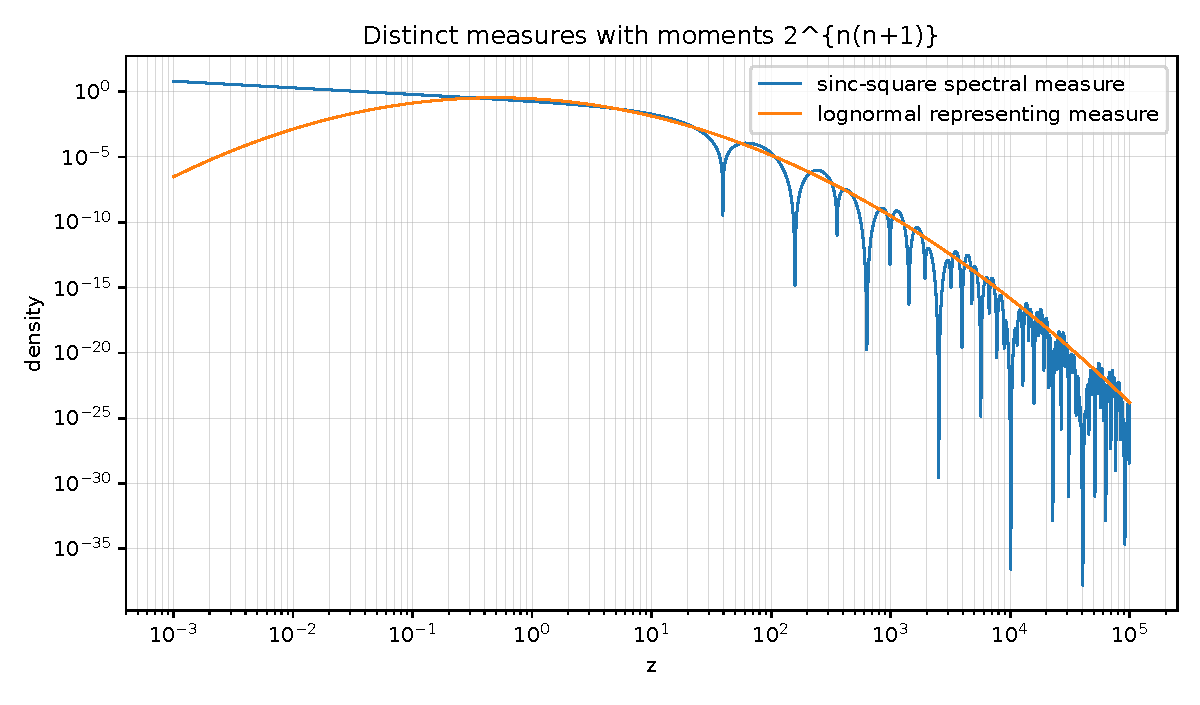
\includegraphics[width=0.91\textwidth]{assets/Fabius_Derivative_Norm_Spectrum_bundle/figures/spectral_vs_lognormal.pdf}
\caption{The sinc-square spectral density and a lognormal density have exactly the same
nonnegative integer moments but visibly different local structures.  The spectral zeros are
inherited from the integer zeros of the infinite sinc product.}
\label{p4:fig:spectral-vs-lognormal}
\end{figure}

\subsection{A nonclassical q-Pearson equation}

The Fourier product satisfies
\begin{equation}
 \Phi(2\xi)=\sinc(2\pi\xi)\Phi(\xi).
 \label{p4:eq:Phi-scaling}
\end{equation}

\begin{proposition}[Sinc-square q-Pearson law]
\label{p4:prop:q-Pearson}
The spectral density \eqref{p4:eq:spectral-density} obeys
\begin{equation}
 \boxed{
 w_{\rm sp}(4z)=\frac12\sinc^2(\sqrt z)\,w_{\rm sp}(z).}
 \label{p4:eq:spectral-q-Pearson}
\end{equation}
By contrast, the lognormal representative satisfies
\begin{equation}
 w_{\rm ln}(4z)=\frac1{4z}w_{\rm ln}(z).
 \label{p4:eq:lognormal-q-Pearson}
\end{equation}
\end{proposition}

\begin{proof}
In \eqref{p4:eq:spectral-density}, replacing $z$ by $4z$ doubles the Fourier argument and
multiplies the square-root denominator by $2$.  Apply \eqref{p4:eq:Phi-scaling} and note that
$2\pi(\sqrt z/(2\pi))=\sqrt z$.  The lognormal identity follows by direct substitution in
\eqref{p4:eq:lognormal-density}.
\end{proof}

\begin{remark}
Classical Stieltjes--Wigert measures satisfy q-Pearson equations with monomial or rational
multipliers.  Equation \eqref{p4:eq:spectral-q-Pearson} replaces that multiplier by an entire
sinc-square factor carrying the complete integer-zero divisor.  Determining its position in
the Nevanlinna family is one of the principal open directions in \Cref{p4:sec:future}.
\end{remark}

\section{Hankel determinants, q-binomial polynomials, and Lagrange quadrature}
\label{p4:sec:q-orthogonal}

Fix $0<q<1$ and the moment sequence
\begin{equation}
 m_n=q^{-n(n+1)/2}.
 \label{p4:eq:general-q-moments}
\end{equation}
The Fabius--Rvachev spectral case is $q=1/4$.

\begin{theorem}[Hankel determinants]
\label{p4:thm:Hankel-determinants}
For $N\geq0$,
\begin{equation}
 \boxed{
 \Delta_N:=\det[m_{i+j}]_{i,j=0}^{N}
 =q^{-N(N+1)(4N+5)/6}
 \prod_{k=1}^{N}(q;q)_k,}
 \label{p4:eq:Hankel-determinant}
\end{equation}
where $(q;q)_k=\prod_{r=1}^k(1-q^r)$.
\end{theorem}

\begin{proof}
Factor
\[
 m_{i+j}=q^{-i(i+1)/2}q^{-j(j+1)/2}q^{-ij}.
\]
The row and column factors contribute
$q^{-\sum_{i=0}^N i(i+1)}$.  The remaining determinant is the Vandermonde determinant in
$q^{-i}$:
\[
 \det[(q^{-i})^j]_{i,j=0}^N
 =\prod_{0\leq i<k\leq N}(q^{-k}-q^{-i})
 =q^{-\sum_{k=1}^Nk^2}\prod_{k=1}^{N}(q;q)_k.
\]
Finally
\[
 \sum_{i=1}^{N}i(i+1)+\sum_{i=1}^{N}i^2
 =\frac{N(N+1)(4N+5)}6.
\]
\end{proof}

\begin{theorem}[Monic shifted Stieltjes--Wigert polynomials]
\label{p4:thm:SW-polynomials}
The monic orthogonal polynomial of degree $n$ for any representing measure of
\eqref{p4:eq:general-q-moments} is
\begin{equation}
 \boxed{
 P_n(z)=\sum_{k=0}^{n}
 (-1)^{n-k}q^{k^2-n^2}\qbinom{n}{k}{q}\,z^k.}
 \label{p4:eq:SW-polynomial}
\end{equation}
It satisfies
\begin{equation}
 \int z^jP_n(z)\dd\mu(z)=0,
 \qquad0\leq j<n,
 \label{p4:eq:SW-orthogonality}
\end{equation}
for every measure $\mu$ with moments \eqref{p4:eq:general-q-moments}, and
\begin{equation}
 h_n:=\int P_n(z)^2\dd\mu(z)
 =q^{-(2n^2+n)}(q;q)_n.
 \label{p4:eq:SW-norm}
\end{equation}
The three-term recurrence is
\begin{equation}
 P_{n+1}(z)=(z-a_n)P_n(z)-b_nP_{n-1}(z),
 \label{p4:eq:SW-recurrence}
\end{equation}
with
\begin{align}
 a_n&=q^{-2n-1}(1+q-q^{n+1}),\label{p4:eq:an}\\
 b_n&=q^{-(4n-1)}(1-q^n),\qquad n\geq1.
 \label{p4:eq:bn}
\end{align}
\end{theorem}

\begin{proof}
Let $c_k$ be the coefficient of $z^k$ in \eqref{p4:eq:SW-polynomial}.  For $j<n$,
\begin{align*}
 \sum_{k=0}^{n}c_km_{k+j}
 &=(-1)^nq^{-n^2-j(j+1)/2}
 \sum_{k=0}^{n}(-1)^kq^{k(k-1)/2}
 \qbinom{n}{k}{q}q^{-jk}\\
 &=(-1)^nq^{-n^2-j(j+1)/2}(q^{-j};q)_n=0,
\end{align*}
by the finite q-binomial theorem; one factor is $1-q^0$.  The leading coefficient is one.
The norm is the standard Gram-determinant quotient
$h_n=\Delta_n/\Delta_{n-1}$, which gives \eqref{p4:eq:SW-norm}.  Hence
$b_n=h_n/h_{n-1}$.  Comparing the coefficients of $z^n$ in the monic recurrence gives
$a_n$; the coefficient of $z^{n-1}$ in $P_n$ is
$-q^{-2n+1}(1-q^n)/(1-q)$, yielding \eqref{p4:eq:an}.
\end{proof}

For $q=1/4$, the first polynomials are
\begin{align}
 P_0(z)&=1,\nonumber\\
 P_1(z)&=z-4,\nonumber\\
 P_2(z)&=z^2-80z+256,\nonumber\\
 P_3(z)&=(z-64)(z^2-1280z+4096).
 \label{p4:eq:first-SW-polynomials}
\end{align}

\subsection{Gaussian quadrature as q-binomial Lagrange interpolation}

Let $\lambda_{n,1},\ldots,\lambda_{n,n}$ be the zeros of $P_n$ and let
$\ell_{n,j}$ be the Lagrange cardinal polynomial at these nodes.  The Gaussian weights are
\begin{equation}
 \omega_{n,j}:=\int\ell_{n,j}(z)\dd\mu(z)
 =\left(\sum_{r=0}^{n-1}\frac{P_r(\lambda_{n,j})^2}{h_r}\right)^{-1}.
 \label{p4:eq:Christoffel-weights}
\end{equation}
Because the polynomials and $h_r$ are determined by the moment sequence, the nodes and
weights are identical for $\mu_{\rm sp}$, the lognormal measure, and every other representing
measure.

\begin{corollary}[Measure-independent Gaussian quadrature]
\label{p4:cor:Gaussian-quadrature}
For every polynomial $Q$ of degree at most $2n-1$,
\begin{equation}
 \boxed{
 \int_0^\infty Q(z)\dd\mu_{\rm sp}(z)
 =\sum_{j=1}^{n}\omega_{n,j}Q(\lambda_{n,j})
 =\int_0^\infty Q(z)w_{\rm ln}(z)\dd z.}
 \label{p4:eq:Gaussian-quadrature}
\end{equation}
The q-binomial coefficients in \eqref{p4:eq:SW-polynomial} therefore generate exact finite
Lagrange quadrature rules for polynomial spectral energies of the infinite sinc product.
\end{corollary}

\begin{remark}
Moment indeterminacy is invisible to every finite polynomial test: all representing measures
produce the same Gaussian quadrature.  The distinction lives in the orthogonal complement of
the polynomial closure, exactly where the integer-zero geometry of $\Phi$ can enter.
\end{remark}

\section{The optimal derivative weight and a q-Legendre Fourier envelope}
\label{p4:sec:carleman}

\subsection{Exact Denjoy--Carleman weight}

Define
\begin{equation}
 M_n:=2^{T_n}=2^{n(n+1)/2}.
 \label{p4:eq:Mn}
\end{equation}
By \eqref{p4:eq:Linf-exact}, $\Up$ saturates this derivative weight exactly:
\begin{equation}
 \norm{\Up^{(n)}}_\infty=M_n.
 \label{p4:eq:saturates-Mn}
\end{equation}
The sequence is logarithmically convex and
\begin{equation}
 \frac{M_n}{M_{n+1}}=2^{-(n+1)},
 \qquad
 \sum_{n=0}^{\infty}\frac{M_n}{M_{n+1}}=1<\infty.
 \label{p4:eq:nonquasianalytic-sum}
\end{equation}
Thus the direct-weight Denjoy--Carleman class generated by $M$ is nonquasianalytic, as the
existence of the compactly supported nonzero function $\Up$ requires.

\begin{proposition}[Outside every finite Gevrey class]
\label{p4:prop:not-Gevrey}
For no finite $s>0$ do constants $A,C>0$ satisfy
\begin{equation}
 M_n\leq CA^n(n!)^s\qquad(n\geq0).
 \label{p4:eq:no-Gevrey-bound}
\end{equation}
Hence $\Up$ belongs to no finite-order Gevrey class on any interval containing its support.
\end{proposition}

\begin{proof}
The logarithm of $M_n$ is $(\log2)n^2/2+\bigO(n)$, whereas
$\log((n!)^sA^n)=sn\log n+\bigO(n)$.  The quadratic term wins.
\end{proof}

\subsection{Exact associated function and periodic lattice correction}

Define the associated function
\begin{equation}
 \omega_M(t):=\sup_{n\geq0}\log\frac{t^n}{M_n},
 \qquad t>0.
 \label{p4:eq:associated-function}
\end{equation}
Let $r=\log_2t$.

\begin{theorem}[Exact q-Legendre transform]
\label{p4:thm:q-Legendre}
For $r\geq1/2$,
\begin{equation}
 \boxed{
 \omega_M(t)=\frac{\log2}{2}
 \left[
 \left(r-\frac12\right)^2
 -\dist\!\left(r-\frac12,\N_0\right)^2
 \right].}
 \label{p4:eq:q-Legendre}
\end{equation}
For $r\leq1/2$, $\omega_M(t)=0$.  Thus the continuous log-square Legendre transform carries
an exact bounded one-periodic lattice correction in $\log_2t$.
\end{theorem}

\begin{proof}
For each integer $n\geq0$,
\[
 \log\frac{t^n}{M_n}
 =\log2\left(nr-\frac{n(n+1)}2\right)
 =\frac{\log2}{2}\left[
 \left(r-\frac12\right)^2-
 \left(n-r+\frac12\right)^2\right].
\]
Maximizing means choosing the nearest nonnegative integer to $r-1/2$.  If $r\leq1/2$, the
maximum is attained at $n=0$ and equals zero.
\end{proof}

\begin{corollary}[Optimized integration-by-parts envelope]
\label{p4:cor:IBP-envelope}
For every $\xi\neq0$,
\begin{equation}
 \boxed{
 |\Phi(\xi)|
 \leq\inf_{n\geq0}\frac{M_n}{(2\pi|\xi|)^n}
 =\exp\bigl(-\omega_M(2\pi|\xi|)\bigr).}
 \label{p4:eq:IBP-envelope}
\end{equation}
If $r=\log_2(2\pi|\xi|)\geq1/2$, this is
\begin{equation}
 |\Phi(\xi)|\leq
 2^{-\frac12(r-1/2)^2+\frac12\dist(r-1/2,\N_0)^2}.
 \label{p4:eq:explicit-IBP-envelope}
\end{equation}
\end{corollary}

\begin{proof}
Integrating the Fourier transform by parts $n$ times and using
\eqref{p4:eq:L1-exact} gives
$|\Phi(\xi)|\leq M_n/(2\pi|\xi|)^n$.  Optimize with
\Cref{p4:thm:q-Legendre}.
\end{proof}

\begin{warning}
The envelope \eqref{p4:eq:explicit-IBP-envelope} is the best one obtainable from the exact
$L^1$ derivative norms alone; it is not the sharp pointwise or annular Fourier envelope.
The Fourier-decay reports in the corpus exploit the lacunary sine cocycle and obtain stronger
linear-in-$\log|\xi|$ corrections.  The value of \eqref{p4:eq:explicit-IBP-envelope} is its exact
functional-analytic duality with the derivative weight, not a replacement for those sharper
results.
\end{warning}

\section{Numerical experiments}
\label{p4:sec:numerics}

All code used here is in \texttt{numerical\_experiments.py}.  It is included with detailed
comments in the accompanying archive.  The script reconstructs $\Up$ by inverse FFT on a
periodic box of length $4$ from $55$ dyadic sinc factors, using $2^{19}$ samples.  Since
$\Up$ is supported on $[-1,1]$, the box supplies exact geometric zero padding.  The run used
\[
 \Delta x=2^{-17}=7.62939453125\times10^{-6},
 \qquad \Delta\xi=\frac14.
\]
The reconstructed density had integral $1$ and value $\Up(0)=1$ to displayed precision;
the largest value outside the support was $3.33\times10^{-16}$.

\subsection{Derivative tiling and norm checks}

\begin{figure}[htbp]
\centering
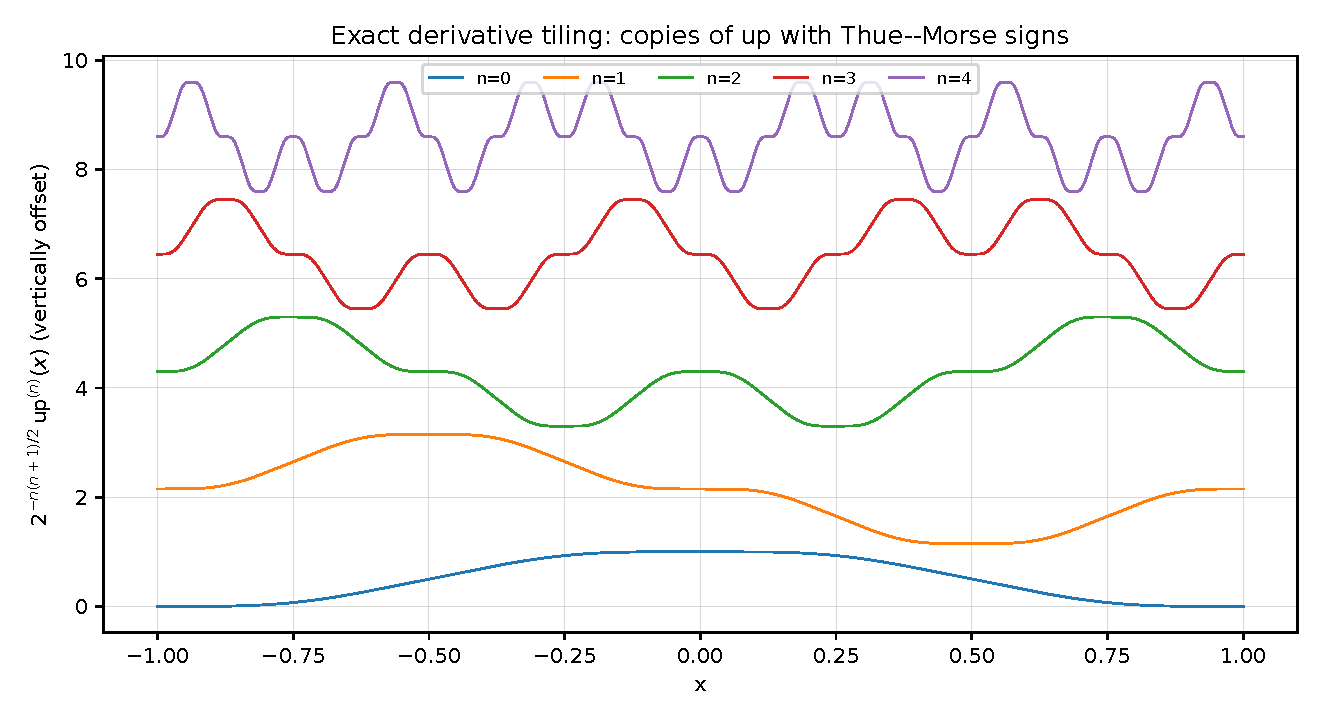
\includegraphics[width=0.94\textwidth]{assets/Fabius_Derivative_Norm_Spectrum_bundle/figures/derivative_tiling.pdf}
\caption{Normalized derivatives $2^{-T_n}\Up^{(n)}$, vertically offset.  Each row is a
concatenation of copies of the original bump; their signs are the length-$2^n$ Thue--Morse
block.}
\label{p4:fig:derivative-tiling}
\end{figure}

For $n=0,\ldots,6$ and $p\in\{1,2,4,8,\infty\}$, the script formed the derivative from the
exact cell formula and compared its numerical norm with
$2^{T_n}\norm{\Up}_p$.  The largest absolute deviation of the ratio from $1$ was
$2.22\times10^{-16}$.

\subsection{Spectral moments}

\begin{center}
\small
\begin{tabular}{@{}rrrr@{}}
\toprule
$n$ & numerical $\int(2\pi\xi)^{2n}|\Phi|^2$ & predicted $2^{n(n+1)}C_2$ & relative error\\
\midrule
0 & $8.088735359679706\times10^{-1}$ & $8.088735359679707\times10^{-1}$ & $-1.11\times10^{-16}$\\
1 & $3.235494143871882$ & $3.235494143871883$ & $-2.22\times10^{-16}$\\
2 & $5.176790630195011\times10^{1}$ & $5.176790630195013\times10^{1}$ & $-2.22\times10^{-16}$\\
3 & $3.313146003324810\times10^{3}$ & $3.313146003324808\times10^{3}$ & $4.44\times10^{-16}$\\
4 & $8.481653768511517\times10^{5}$ & $8.481653768511509\times10^{5}$ & $8.88\times10^{-16}$\\
5 & $8.685213458955796\times10^{8}$ & $8.685213458955785\times10^{8}$ & $1.33\times10^{-15}$\\
6 & $3.557463432788293\times10^{12}$ & $3.557463432788290\times10^{12}$ & $8.88\times10^{-16}$\\
7 & $5.828548088280333\times10^{16}$ & $5.828548088280334\times10^{16}$ & $-1.11\times10^{-16}$\\
\bottomrule
\end{tabular}
\end{center}

The near-machine equality is a stringent joint check of the FFT normalization, derivative
scale, Parseval convention, and moment exponent.

\subsection{Euler--Gamma operator convergence}

The inverse interpolant was obtained directly from
$G(1-\Up(x))=x$ on $0\leq x\leq1$.  Logarithmic finite differences estimated
$\Dop^kG(1/p)$ for $k\leq3$.  The following table lists relative errors of successive
truncations of \eqref{p4:eq:Gamma-operator-first-terms}.

\begin{center}
\small
\begin{tabular}{@{}rrrrrr@{}}
\toprule
$p$ & $A_p/G(1/p)$ & $G$ only & through $\Dop$ & through $\Dop^2$ & through $\Dop^3$\\
\midrule
256   & 0.92618125 & $-7.38\!\times10^{-2}$ & $4.84\!\times10^{-2}$ & $-1.47\!\times10^{-2}$ & $6.46\!\times10^{-3}$\\
512   & 0.92793214 & $-7.21\!\times10^{-2}$ & $4.32\!\times10^{-2}$ & $-1.20\!\times10^{-2}$ & $6.37\!\times10^{-3}$\\
1024  & 0.92942377 & $-7.06\!\times10^{-2}$ & $3.91\!\times10^{-2}$ & $-9.78\!\times10^{-3}$ & $4.87\!\times10^{-3}$\\
2048  & 0.93089393 & $-6.91\!\times10^{-2}$ & $3.60\!\times10^{-2}$ & $-8.37\!\times10^{-3}$ & $3.35\!\times10^{-3}$\\
4096  & 0.93235311 & $-6.76\!\times10^{-2}$ & $3.33\!\times10^{-2}$ & $-7.55\!\times10^{-3}$ & $2.53\!\times10^{-3}$\\
8192  & 0.93370939 & $-6.63\!\times10^{-2}$ & $3.09\!\times10^{-2}$ & $-6.86\!\times10^{-3}$ & $2.39\!\times10^{-3}$\\
16384 & 0.93492704 & $-6.51\!\times10^{-2}$ & $2.87\!\times10^{-2}$ & $-6.10\!\times10^{-3}$ & $2.29\!\times10^{-3}$\\
32768 & 0.93604971 & $-6.40\!\times10^{-2}$ & $2.69\!\times10^{-2}$ & $-5.39\!\times10^{-3}$ & $1.97\!\times10^{-3}$\\
65536 & 0.93712995 & $-6.29\!\times10^{-2}$ & $2.53\!\times10^{-2}$ & $-4.83\!\times10^{-3}$ & $1.60\!\times10^{-3}$\\
\bottomrule
\end{tabular}
\end{center}

\begin{figure}[htbp]
\centering
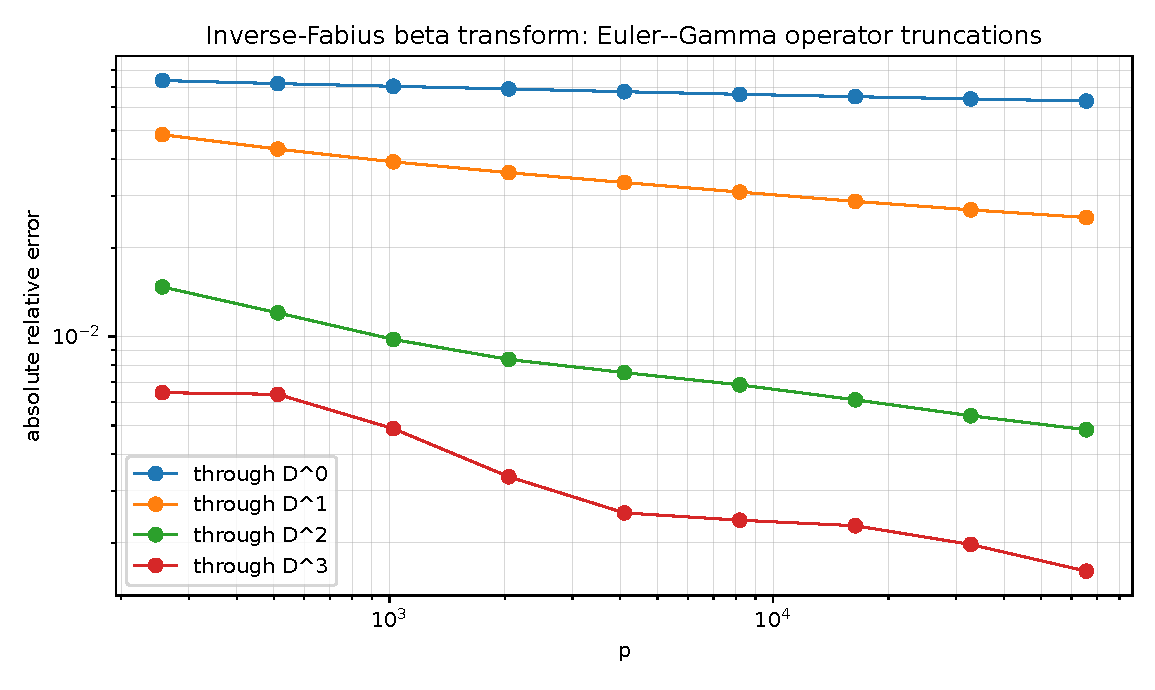
\includegraphics[width=0.87\textwidth]{assets/Fabius_Derivative_Norm_Spectrum_bundle/figures/beta_operator_errors.pdf}
\caption{Absolute relative errors of the first four Euler--Gamma operator truncations.  The
slow scale $\rho^{-1}\asymp(\log p)^{-1/2}$ explains why very large $p$ is needed before
successive asymptotic orders separate cleanly.}
\label{p4:fig:beta-errors}
\end{figure}

\subsection{Symbolic Hankel checks}

SymPy evaluated the determinants in \eqref{p4:eq:Hankel-determinant} exactly for
$N=0,\ldots,6$ at $q=1/4$; every quotient of the direct determinant by the claimed closed
form simplified to $1$.  The base-$10$ logarithms of the determinants for $N=1,\ldots,6$
were
\[
 1.68124,\ 7.54887,\ 20.03233,\ 41.54498,\ 74.49635,\ 121.29499,
\]
illustrating the rapid $q^{-\frac23N^3+\bigO(N^2)}$ growth.

\section{Conjectures and promising research directions}
\label{p4:sec:future}

\subsection{A full norm transseries}

The inverse report gives an all-orders expansion of $G$ in the differential algebra generated
by periodic saddle jets.  The exact operator \eqref{p4:eq:exact-operator} should transport that
algebra to the norm spectrum without introducing any new transcendental data beyond the
log-exponential cumulants.

\begin{conjecture}[All-orders Gamma--Lambert norm transseries]
\label{p4:conj:full-norm-transseries}
There exist one-periodic real-analytic coefficient functions
$C_{m,\ell}(\theta)$ such that
\begin{equation}
 \frac{\norm{\Up}_p^p}{2G_0(p^{-1})}
 \sim1+\sum_{m=1}^{\infty}\rho^{-m}
 \sum_{\ell=0}^{m}C_{m,\ell}(\theta)(\log\rho)^\ell,
 \label{p4:eq:full-norm-transseries}
\end{equation}
with $C_{1,1}=1/2$ and
$C_{1,0}=\kappa_0-\gamma-\Psi(\theta)$.  Every $C_{m,\ell}$ belongs to the differential
algebra generated by the inverse saddle jets and the constants
$\gamma,\zeta(2),\ldots,\zeta(m)$; no additional periodic functions occur.
\end{conjecture}

A proof should combine the formal inverse recursion already in the corpus with a tame
remainder theorem for the operator $M_p(\Dop)$.  The key analytic task is uniform control of
$\Dop^mG$ on logarithmic windows whose width grows slowly with $\rho$.

\subsection{Nevanlinna parameter of the sinc-square measure}

\begin{problem}[Locate $\mu_{\rm sp}$ in the Stieltjes--Wigert Nevanlinna family]
\label{p4:prob:Nevanlinna}
Determine the Nevanlinna parameter corresponding to the density
\eqref{p4:eq:spectral-density}.  Equivalently, calculate the Cauchy transform
\begin{equation}
 S_{\rm sp}(z)=\int_0^\infty\frac{\dd\mu_{\rm sp}(t)}{z-t}
 \label{p4:eq:spectral-Stieltjes-transform}
\end{equation}
relative to the classical entire functions $A,B,C,D$ of the shifted
Stieltjes--Wigert moment problem.
\end{problem}

The exact q-Pearson law \eqref{p4:eq:spectral-q-Pearson} supplies unusually rigid extra data.
One promising route is to Mellin-transform it, obtaining a functional equation coupling the
spectral Mellin transform to the Mellin transform of $\sinc^2(\sqrt z)$.  Another is to use
the canonical product of $\Phi$ to express $S_{\rm sp}$ as a convergent sum over integer-zero
lobes.

\begin{conjecture}[Sinc-Pearson uniqueness]
\label{p4:conj:sinc-Pearson-uniqueness}
Among absolutely continuous representing measures of
$m_n=2^{n(n+1)}$ whose density is locally bounded after multiplication by $\sqrt z$, the
normalization, moment conditions, and q-Pearson equation
\eqref{p4:eq:spectral-q-Pearson} determine $w_{\rm sp}$ uniquely.
\end{conjecture}

\subsection{Orthogonal complement and spectral zeros}

For an indeterminate moment problem, the polynomials are not dense in every representing
$L^2$ space.  The spectral measure should possess an orthogonal complement reflecting the
integer-zero structure of $\Phi$.

\begin{problem}[Explicit nonpolynomial orthogonal basis]
Construct functions $Q_j(z)$ such that
\[
 \int_0^\infty z^nQ_j(z)w_{\rm sp}(z)\dd z=0
 \qquad(n\geq0)
\]
and such that the $Q_j$ span the orthogonal complement of the shifted
Stieltjes--Wigert polynomials in $L^2(\mu_{\rm sp})$.  Dyadic rescalings of sinc factors,
integer-lobe indicator functions, and q-Bessel functions from the classical theory are the
three natural candidate families.
\end{problem}

\subsection{Confluent q-Richardson phase tomography}

The existing corpus develops Gaussian-q Richardson weights for pure power error germs.
The norm expansion \eqref{p4:eq:full-norm-transseries} contains powers multiplied by logarithms.
Choose a fixed phase $\vartheta$ and a dyadic phase-locked sequence
\begin{equation}
 \rho_j=M2^j+\delta,
 \qquad
 \delta+\beta\equiv\vartheta\pmod1,
 \qquad
 p_j=\exp(L\rho_j^2/2).
 \label{p4:eq:dyadic-phase-nodes}
\end{equation}
Then $h_j=1/\rho_j$ is an analytic function of $2^{-j}$, while the phase is constant.
After subtracting the known logarithmic terms, the remaining errors are combinations of
$j^\ell2^{-mj}$.

\begin{conjecture}[Confluent Gaussian-q filter]
\label{p4:conj:confluent-q-filter}
For each truncation order $r$, there is a stable finite filter whose shift polynomial is a
product of repeated factors
\begin{equation}
 \prod_{m=1}^{r}(E-2^{-m})^{d_m},
 \label{p4:eq:confluent-shift-polynomial}
\end{equation}
which annihilates every error mode $j^\ell2^{-mj}$ with
$0\leq\ell<d_m$.  Its coefficients can be written as derivatives or confluent limits of the
Gaussian-q-binomial Lagrange weights
\begin{equation}
 w_{r,j}(q)=(-1)^{r-j}
 \frac{q^{\binom{r-j+1}{2}}}{(q;q)_j(q;q)_{r-j}}.
 \label{p4:eq:q-Richardson-weights}
\end{equation}
Applied to \eqref{p4:eq:dyadic-phase-nodes}, this filter recovers
$\kappa_0-\gamma-\Psi(\vartheta)$ with a rigorously controlled error of arbitrarily high
order in $2^{-j}$.
\end{conjecture}

This would create a genuinely new Richardson pipeline: the data are global derivative norms,
the target is a pointwise endpoint periodic function, and the logarithmic multiplicities are
handled by confluent q-Lagrange interpolation.

\subsection{Base-b and Pascal--Rvachev extensions}

The Pascal--Rvachev hierarchy in the corpus replaces the single sinc exponent by binomial
multiplicities.  The present analysis suggests two extensions.

\begin{problem}[Norm ladders for higher Rvachev ranks]
For each hierarchy level, identify a spatial refinement formula with disjoint or finitely
overlapping cells, determine whether normalized derivatives are equimeasurable with a fixed
profile, and calculate the resulting derivative weight.  If exact equimeasurability fails,
seek a finite-state transfer operator for value distributions.
\end{problem}

\begin{conjecture}[Higher-rank lognormal moment geometry]
For the rank-$r$ Pascal--Rvachev profile, the normalized spectral energy moments are
$q$-hyperfactorial sequences whose Hankel determinants factor into products of
$q$-Pochhammer symbols with exponents polynomial in the index.  The associated orthogonal
polynomials should be multilevel q-binomial deformations of Stieltjes--Wigert polynomials.
\end{conjecture}

\subsection{Formalization roadmap}

The roadmap is now partly discharged.  The completion labels below refer only to the named
declarations in \path{RvachevDerivativeDistribution.lean}; they do not mark the whole report
as formalized.  A practical order is:
\begin{enumerate}
\item \textbf{Completed.}  The derivative tiling has a public exact cell coordinate,
      endpoint/range lemmas, signed and absolute cellwise formulas, and signed midpoint
      corollary.
\item \textbf{Absolute part completed.}  The normalized absolute law is an exact Borel
      pushforward equality and has Banach-valued continuous-test forms.  The signed
      finite-mixture identity is also formal for continuous Banach-valued tests and all
      \(n\), but its simplified signed Rademacher Borel law remains open.
\item \textbf{Still open beyond completed prerequisites.}  Use the all-\(p\ge0\)
      real-power moment theorem, midpoint signs, and existing pointwise bounds to derive
      \path{eLpNorm}, general rearrangement-invariant, total-variation, and exact
      inverse-Fabius level-set corollaries.
\item \textbf{Open.}  Formalize the Stieltjes substitution and beta-transform identity for
      the totalized inverse.
\item \textbf{Open.}  Prove the spectral moments by the existing Fourier differentiation
      API.
\item \textbf{Open.}  Formalize the Vandermonde determinant and finite q-binomial
      orthogonality.
\item \textbf{Deferred.}  Treat the all-orders asymptotic operator after the inverse
      derivative-jet bounds have a stable public interface.
\end{enumerate}

\section{Conclusion}

The dyadic derivative formula contains more information than its usual pointwise reading
suggests.  Because the cells are disjoint and all have the same affine Jacobian, it is an
exact renormalization fixed point for value distributions.  The entire derivative tower has
one absolute profile, amplified by $2^{n(n+1)/2}$ and signed by Thue--Morse.  This immediately
produces an exact norm spectrum in every rearrangement-invariant space and makes the inverse
Fabius function the level-set law of every derivative.

Two dual transforms then emerge.  In physical space, the large-$p$ norms are a beta average
of the inverse function.  The beta dilation converges to an exponential dilation, whose
Mellin symbol is $\Gamma(1+s)$; Bell polynomials, zeta values, and Bernoulli polynomials are
therefore forced into the asymptotic operator.  Combining it with the lower-Lambert endpoint
coordinate reveals a universal Euler-constant shift and lets global norms perform phase
tomography on the periodic saddle correction.

In frequency space, Parseval turns the same derivative scale into the moment sequence
$2^{n(n+1)}$.  The infinite sinc product thus supplies an explicit, highly nonclassical
Stieltjes--Wigert representing measure.  Its integer zeros distinguish it from the lognormal
representative even though all polynomial moments agree; its q-Pearson law retains the full
sinc-square factor.  The resulting q-binomial orthogonal polynomials and Gaussian Lagrange
rules give a concrete bridge between spectral energy, moment indeterminacy, and the
$q$-calculus already pervasive in the Fabius theory.

The most promising analytic next step is to identify the sinc-square measure inside the
Nevanlinna family.  On the formal side, the dyadic-cell and normalized absolute
equimeasurability core is now complete.  The next compact targets are its
\path{eLpNorm}/rearrangement-invariant and inverse-Fabius level-set consequences, followed
by the beta-transform layer.  The signed Rademacher Borel simplification and every
beta/spectral layer in this report remain frontier statements.

\appendix

\section{Recursive TeX corpus ledger}
\label{p4:app:corpus-ledger}

The following $68$ paths were present under
\path{Analysis/FabiusFunction/docs} at commit \RepoCommit.  Archived versions were included
in the collision audit but interpreted according to the archive's provenance ledger.

\begingroup
\small
\renewcommand{\arraystretch}{1.08}
\begin{longtable}{@{}r>{\raggedright\arraybackslash}p{0.88\textwidth}@{}}
\toprule
\# & Path\\
\midrule
\endfirsthead
\toprule
\# & Path (continued)\\
\midrule
\endhead
1 & \path{FabiusFunction_Mathematical_Glossary/FabiusFunction_Mathematical_Glossary.tex}\\
2 & \path{Fabius_Function_and_Rvachev_Up/Fabius_Function_and_Rvachev_Up.tex}\\
3 & \path{Non_Elementarity_of_the_Fabius_Function/Non_Elementarity_of_the_Fabius_Function.tex}\\
4 & \path{archive/early-notes/Fabius Asymptotic/Fabius Asymptotic.tex}\\
5 & \path{archive/early-notes/K-fold summation over the signed Thue-Morse sequence/K-fold summation over the signed Thue-Morse sequence.tex}\\
6 & \path{archive/glossary/FabiusFunction_Mathematical_Glossary-2/FabiusFunction_Mathematical_Glossary.tex}\\
7 & \path{archive/glossary/FabiusFunction_Mathematical_Glossary/FabiusFunction_Mathematical_Glossary.tex}\\
8 & \path{archive/lean-walkthrough/Fabius_Function_Lean_Walkthrough/Fabius_Function_Lean_Walkthrough.tex}\\
9 & \path{archive/lean-walkthrough/fabius_lean_walkthrough/fabius_lean_walkthrough.tex}\\
10 & \path{archive/primary-exposition/Fabius_Function_and_Rvachev_Up-2/Fabius_Function_and_Rvachev_Up.tex}\\
11 & \path{archive/primary-exposition/Fabius_Function_and_Rvachev_Up-3/Fabius_Function_and_Rvachev_Up.tex}\\
12 & \path{archive/primary-exposition/Fabius_Function_and_Rvachev_Up/Fabius_Function_and_Rvachev_Up.tex}\\
13 & \path{archive/primary-exposition/Fabius_and_Rvachev_Up-2/Fabius_and_Rvachev_Up.tex}\\
14 & \path{archive/primary-exposition/Fabius_and_Rvachev_up/Fabius_and_Rvachev_up.tex}\\
15 & \path{archive/primary-exposition/Fabius_function_and_up_function/Fabius_function_and_up_function.tex}\\
16 & \path{archive/primary-supplements/Fabius_Function_Missing_Parts-2/Fabius_Function_Missing_Parts.tex}\\
17 & \path{archive/primary-supplements/Fabius_Function_Missing_Parts/Fabius_Function_Missing_Parts.tex}\\
18 & \path{archive/q-calculus/Fabius_q_Special_Functions/Fabius_q_Special_Functions.tex}\\
19 & \path{archive/q-calculus/fabius-q-special-functions/fabius-q-special-functions.tex}\\
20 & \path{archive/research-frontiers/Fabius_Dyadic_Asymptotic_Bridge/Fabius_Dyadic_Asymptotic_Bridge.tex}\\
21 & \path{archive/research-frontiers/Fabius_Dyadic_Formulae_and_Alternative_Representations/Fabius_Dyadic_Formulae_and_Alternative_Representations.tex}\\
22 & \path{archive/research-frontiers/Fabius_Dyadic_Formulae_to_Asymptotics/Fabius_Dyadic_Formulae_to_Asymptotics.tex}\\
23 & \path{archive/research-frontiers/Fabius_Dyadic_q_Connections/Fabius_Dyadic_q_Connections.tex}\\
24 & \path{archive/research-frontiers/Fabius_Thue_Morse_Convergence_Rate/Fabius_Thue_Morse_Convergence_Rate.tex}\\
25 & \path{archive/research-frontiers/Fabius_Thue_Morse_Convergence_Rates/Fabius_Thue_Morse_Convergence_Rates.tex}\\
26 & \path{archive/research-frontiers/Primary_Exposition_Gap_Register/Primary_Exposition_Gap_Register.tex}\\
27 & \path{archive/research-frontiers/Repeated_Integration_and_Rvachev_Up/Repeated_Integration_and_Rvachev_Up.tex}\\
28 & \path{archive/research-frontiers/Rvachev_Up_from_Repeated_Integration/Rvachev_Up_from_Repeated_Integration.tex}\\
29 & \path{archive/research-frontiers/Thue_Morse_Formula_Atlas-1/Thue_Morse_Formula_Atlas.tex}\\
30 & \path{archive/research-frontiers/Thue_Morse_Formula_Atlas-2/Consolidated_Formula_Atlas_for_the_Thue_Morse_Sequence.tex}\\
31 & \path{archive/research-frontiers/Thue_Morse_Formula_Atlas-3/Thue_Morse_Formula_Atlas.tex}\\
32 & \path{archive/research-frontiers/non-formalized-research-frontiers/semi-formalized-research-frontiers.tex}\\
33 & \path{archive/standalone-studies/Non_Elementarity_of_the_Fabius_Function/Non_Elementarity_of_the_Fabius_Function.tex}\\
34 & \path{archive/standalone-studies/Small_Argument_Asymptotics/Small_Argument_Asymptotics.tex}\\
35 & \path{archive/standalone-studies/fabius-inverse-dyadic-closed-form/fabius-inverse-dyadic-closed-form.tex}\\
36 & \path{fabius_lean_walkthrough/fabius_lean_walkthrough.tex}\\
37 & \path{semi-formalized-research-frontiers/semi-formalized-research-frontiers.tex}\\
38 & \path{semi-formalized-research-frontiers/drafts/Fabius_Arithmetic_Rays_Frontier_Report/Fabius_Arithmetic_Rays_Frontier_Report.tex}\\
39 & \path{semi-formalized-research-frontiers/drafts/Fabius_Half_Integer_Spectral_Frontier_Report/Fabius_Half_Integer_Spectral_Frontier_Report.tex}\\
40 & \path{semi-formalized-research-frontiers/drafts/Fabius_Inverse_Frontier_Report_Source_and_PDF/Fabius_Inverse_Frontier_Report.tex}\\
41 & \path{semi-formalized-research-frontiers/drafts/Fabius_Rvachev_Frontier_Report-2/Fabius_Rvachev_Frontier_Report.tex}\\
42 & \path{semi-formalized-research-frontiers/drafts/Fabius_Rvachev_Frontier_Report/Fabius_Rvachev_Frontier_Report.tex}\\
43 & \path{semi-formalized-research-frontiers/drafts/Fabius_Rvachev_New_Frontiers/Fabius_Rvachev_New_Frontiers.tex}\\
44 & \path{semi-formalized-research-frontiers/drafts/Fabius_Rvachev_Thue_Morse_Frontier_Results/Fabius_Rvachev_Thue_Morse_Frontier_Results.tex}\\
45 & \path{semi-formalized-research-frontiers/drafts/Spectral_Arithmetic_Pascal_Rvachev_Hierarchy/Spectral_Arithmetic_Pascal_Rvachev_Hierarchy.tex}\\
46 & \path{semi-formalized-research-frontiers/drafts/Thue_Morse_Formula_Atlas/Thue_Morse_Formula_Atlas.tex}\\
47 & \path{semi-formalized-research-frontiers/drafts/fabius_frontier_new_results/fabius_frontier_new_results.tex}\\
48 & \path{semi-formalized-research-frontiers/drafts/fabius_frontier_results_bundle/fabius_frontier_results.tex}\\
49 & \path{semi-formalized-research-frontiers/drafts/fabius_frontier_spectral_endpoint_report_bundle/fabius_frontier_spectral_endpoint_report.tex}\\
50 & \path{semi-formalized-research-frontiers/drafts/rvachev_up_fourier_decay/Rvachev_Up_Fourier_Decay-2/Rvachev_Up_Fourier_Decay.tex}\\
51 & \path{semi-formalized-research-frontiers/drafts/rvachev_up_fourier_decay/Rvachev_Up_Fourier_Decay-3/Fourier_decay_of_Rvachev_up.tex}\\
52 & \path{semi-formalized-research-frontiers/drafts/rvachev_up_fourier_decay/Rvachev_Up_Fourier_Decay_Comparative_Audit/Rvachev_Up_Fourier_Decay_Comparative_Audit.tex}\\
53 & \path{semi-formalized-research-frontiers/drafts/rvachev_up_fourier_decay/Rvachev_Up_Fourier_Decay_Gentle_Guide/Rvachev_Up_Fourier_Decay_Gentle_Guide.tex}\\
54 & \path{semi-formalized-research-frontiers/drafts/rvachev_up_fourier_decay/Rvachev_Up_Fourier_Decay_Second_Wave_Audit/Rvachev_Up_Fourier_Decay_Second_Wave_Audit.tex}\\
55 & \path{semi-formalized-research-frontiers/drafts/rvachev_up_fourier_decay/asymptotic-decay-rate-of-an-infinite-product-of-sinc-functions/asymptotic-decay-rate-of-an-infinite-product-of-sinc-functions.tex}\\
56 & \path{semi-formalized-research-frontiers/drafts/rvachev_up_fourier_decay/rvachev_up_fourier_decay-1/rvachev_up_fourier_decay.tex}\\
57 & \path{semi-formalized-research-frontiers/drafts/rvachev_up_fourier_decay/rvachev_up_fourier_decay-4/rvachev_up_fourier_decay.tex}\\
58 & \path{semi-formalized-research-frontiers/drafts/rvachev_up_fourier_decay/rvachev_up_fourier_decay-5/Rvachev_Up_Fourier_Decay_Final.tex}\\
59 & \path{semi-formalized-research-frontiers/drafts/rvachev_up_fourier_decay/rvachev_up_fourier_decay-6/Rvachev_Up_Fourier_Decay_Final_Synthesis.tex}\\
60 & \path{semi-formalized-research-frontiers/drafts/rvachev_up_fourier_decay/rvachev_up_fourier_decay-7/rvachev_up_fourier_decay_final.tex}\\
61 & \path{semi-formalized-research-frontiers/drafts/rvachev_up_fourier_decay/rvachev_up_fourier_decay-8/rvachev_up_fourier_decay_final.tex}\\
62 & \path{papers/AIF_2017__67_2_637_0/AIF_2017__67_2_637_0-corrected.tex}\\
63 & \path{papers/AIF_2017__67_2_637_0/AIF_2017__67_2_637_0.tex}\\
64 & \path{papers/arXiv-1502.06738v2/Lacunary_products.tex}\\
65 & \path{papers/arXiv-1702.05442v1/09-Function.tex}\\
66 & \path{papers/arXiv-1702.06487v3/157-Arithmetic-v3.tex}\\
67 & \path{papers/arXiv-2211.13570v1/document.tex}\\
68 & \path{papers/ubiq15/ubiq15-corrected.tex}\\
\bottomrule
\end{longtable}
\endgroup

\section{Reproducibility files}
\label{p4:app:reproducibility}

The accompanying archive contains:
\begin{itemize}
\item \texttt{Fabius\_Derivative\_Norm\_Spectrum.tex} -- this source;
\item \texttt{Fabius\_Derivative\_Norm\_Spectrum.pdf} -- the rendered report;
\item \texttt{numerical\_experiments.py} -- commented reproduction code;
\item \texttt{figures/} -- PDF and PNG versions of the three generated figures;
\item \texttt{data/derivative\_norm\_ratios.csv};
\item \texttt{data/spectral\_moment\_checks.csv};
\item \texttt{data/beta\_operator\_checks.csv};
\item \texttt{data/hankel\_determinant\_checks.csv}; and
\item \texttt{data/run\_summary.txt}.
\end{itemize}

The default reproduction command is
\begin{lstlisting}[style=code,language=bash]
python numerical_experiments.py
\end{lstlisting}
The grid size, number of sinc factors, derivative order, and output directory are configurable
through command-line options documented by
\begin{lstlisting}[style=code,language=bash]
python numerical_experiments.py --help
\end{lstlisting}

\begin{thebibliography}{99}

\bibitem{p4:proveit}
V.~Reshetnikov,
\emph{ProveIt: Analysis/FabiusFunction}, repository snapshot at commit
\RepoCommit, 27 August 2026.
\url{https://github.com/VladimirReshetnikov/ProveIt/tree/0341bbf91cb867f4510bc8431cf59878208de771/Analysis/FabiusFunction}

\bibitem{p4:arias1982}
J.~Arias de Reyna,
\emph{On the function of Fabius},
English translation and corrected source in
\texttt{docs/papers/AIF\_2017\_\_67\_2\_637\_0}; original Spanish article,
\emph{Revista de la Real Academia de Ciencias Exactas, F\'isicas y Naturales de Madrid}
\textbf{76} (1982), 367--376.

\bibitem{p4:arias2018}
J.~Arias de Reyna,
\emph{Arithmetic of the Fabius function},
\emph{Journal de Th\'eorie des Nombres de Bordeaux} \textbf{30} (2018), 721--749;
source imported in \texttt{docs/papers/arXiv-1702.06487v3}.

\bibitem{p4:fabius1966}
J.~Fabius,
\emph{A probabilistic example of a nowhere analytic $C^\infty$-function},
\emph{Zeitschrift f\"ur Wahrscheinlichkeitstheorie und Verwandte Gebiete}
\textbf{5} (1966), 173--174.

\bibitem{p4:jessen-wintner}
B.~Jessen and A.~Wintner,
\emph{Distribution functions and the Riemann zeta function},
\emph{Transactions of the American Mathematical Society} \textbf{38} (1935), 48--88.

\bibitem{p4:chihara1970}
T.~S.~Chihara,
\emph{A characterization and a class of distribution functions for the
Stieltjes--Wigert polynomials},
\emph{Canadian Mathematical Bulletin} \textbf{13} (1970), 529--532.

\bibitem{p4:christiansen2003}
J.~S.~Christiansen,
\emph{The moment problem associated with the Stieltjes--Wigert polynomials},
\emph{Journal of Mathematical Analysis and Applications} \textbf{277} (2003), 218--245.

\bibitem{p4:christiansen-koelink}
J.~S.~Christiansen and E.~Koelink,
\emph{Self-adjoint difference operators and classical solutions to the
Stieltjes--Wigert moment problem},
\emph{Journal of Approximation Theory} \textbf{140} (2006), 1--26;
\url{https://arxiv.org/abs/math/0504456}.

\bibitem{p4:koekoek}
R.~Koekoek, P.~A.~Lesky, and R.~F.~Swarttouw,
\emph{Hypergeometric Orthogonal Polynomials and Their q-Analogues},
Springer, 2010.

\bibitem{p4:berg-regular}
N.~H.~Bingham, C.~M.~Goldie, and J.~L.~Teugels,
\emph{Regular Variation},
Cambridge University Press, 1987.

\bibitem{p4:mandelbrojt}
S.~Mandelbrojt,
\emph{S\'eries adh\'erentes, r\'egularisation des suites, applications},
Gauthier--Villars, Paris, 1952.

\bibitem{p4:nist}
F.~W.~J.~Olver, D.~W.~Lozier, R.~F.~Boisvert, and C.~W.~Clark, editors,
\emph{NIST Handbook of Mathematical Functions},
Cambridge University Press, 2010.

\bibitem{p4:popa-mellin}
D.~Popa,
\emph{The complete asymptotic evaluation for Mellin convolution operators},
\emph{Constructive Approximation} \textbf{58} (2023), 253--270.

\end{thebibliography}


\end{document}
